%
%   This program is free software: you can redistribute it and/or modify
%   it under the terms of the GNU General Public License as published by
%   the Free Software Foundation, either version 3 of the License, or
%   (at your option) any later version.
%
%   This program is distributed in the hope that it will be useful,
%   but WITHOUT ANY WARRANTY; without even the implied warranty of
%   MERCHANTABILITY or FITNESS FOR A PARTICULAR PURPOSE.  See the
%   GNU General Public License for more details.
%
%   You should have received a copy of the GNU General Public License
%   along with this program.  If not, see <http://www.gnu.org/licenses/>.
%

% Version: $Revision$

\documentclass[a4paper]{book}

\usepackage{epsfig}
\usepackage{wrapfig}
\usepackage{graphicx}
\usepackage{hyperref}

%
%   This program is free software: you can redistribute it and/or modify
%   it under the terms of the GNU General Public License as published by
%   the Free Software Foundation, either version 3 of the License, or
%   (at your option) any later version.
%
%   This program is distributed in the hope that it will be useful,
%   but WITHOUT ANY WARRANTY; without even the implied warranty of
%   MERCHANTABILITY or FITNESS FOR A PARTICULAR PURPOSE.  See the
%   GNU General Public License for more details.
%
%   You should have received a copy of the GNU General Public License
%   along with this program.  If not, see <http://www.gnu.org/licenses/>.
%

% $Revision: 8032 $

\hyphenation{Generic-Object-Editor}
\hyphenation{Result-Producer}
\hyphenation{Cross-Validation-Result-Producer}
\hyphenation{Random-Split-Result-Producer}
\hyphenation{Database-Result-Listener}
\hyphenation{DatabaseUtils}

%
%   This program is free software: you can redistribute it and/or modify
%   it under the terms of the GNU General Public License as published by
%   the Free Software Foundation, either version 3 of the License, or
%   (at your option) any later version.
%
%   This program is distributed in the hope that it will be useful,
%   but WITHOUT ANY WARRANTY; without even the implied warranty of
%   MERCHANTABILITY or FITNESS FOR A PARTICULAR PURPOSE.  See the
%   GNU General Public License for more details.
%
%   You should have received a copy of the GNU General Public License
%   along with this program.  If not, see <http://www.gnu.org/licenses/>.
%

% Version: $Revision$

\newenvironment{tight_itemize}{
\begin{itemize}
  \setlength{\itemsep}{1pt}
  \setlength{\parskip}{0pt}
  \setlength{\parsep}{0pt}}{\end{itemize}
}

\newenvironment{tight_enumerate}{
\begin{enumerate}
  \setlength{\itemsep}{1pt}
  \setlength{\parskip}{0pt}
  \setlength{\parsep}{0pt}}{\end{enumerate}
}

% if you just need a simple heading
% Usage:
%   \heading{the text of the heading}
\newcommand{\heading}[1]{
  \vspace{0.3cm} \noindent \textbf{#1} \newline
}



\title{
\epsfig{file=images/coat_of_arms.eps,width=10cm}\vspace{3cm}\\WEKA Manual\\for Version 3-7-10}
\author{Remco R. Bouckaert\\Eibe Frank\\Mark Hall\\Richard Kirkby\\Peter Reutemann\\Alex Seewald\\David Scuse}

\setcounter{secnumdepth}{3}
\setcounter{tocdepth}{3}

\begin{document}

\begin{titlepage}
\maketitle

\thispagestyle{empty}
\center
\begin{table}[b]
\copyright 2002-2013 \\
 \\
University of Waikato, Hamilton, New Zealand \\
Alex Seewald (original Commnd-line primer) \\
David Scuse (original Experimenter tutorial) \\
\\
This manual is licensed under the GNU General Public License version 3. More information about this license can be found at \url{http://www.gnu.org/licenses/gpl-3.0-standalone.html}
\end{table}

\end{titlepage}

\tableofcontents

%%%%%%%%%%%%%%%%%%%%%%%%%%%%%%%%%%%
\part{The Command-line}

\chapter{A command-line primer}
%
%    This program is free software; you can redistribute it and/or modify
%    it under the terms of the GNU General Public License as published by
%    the Free Software Foundation; either version 2 of the License, or
%    (at your option) any later version.
%
%    This program is distributed in the hope that it will be useful,
%    but WITHOUT ANY WARRANTY; without even the implied warranty of
%    MERCHANTABILITY or FITNESS FOR A PARTICULAR PURPOSE.  See the
%    GNU General Public License for more details.
%
%    You should have received a copy of the GNU General Public License
%    along with this program; if not, write to the Free Software
%    Foundation, Inc., 675 Mass Ave, Cambridge, MA 02139, USA.
%

% Version: $Revision$

\section{Introduction}

While for initial experiments the included graphical user interface is quite sufficient, for in-depth usage the command line interface is recommended, because it offers some functionality which is not available via the GUI - and uses far less memory. Should you get \textit{Out of Memory} errors, increase the maximum heap size for your java engine, usually via \texttt{-Xmx1024M} or \texttt{-Xmx1024m} for 1GB - the default setting of 16 to 64MB is usually too small. If you get errors that classes are not found, check your \texttt{CLASSPATH}: does it include \texttt{weka.jar}? You can explicitly set \texttt{CLASSPATH} via the \texttt{-cp} command line option as well.

We will begin by describing basic concepts and ideas. Then, we will describe the \texttt{weka.filters} package, which is used to transform input data, e.g. for preprocessing, transformation, feature generation and so on.

Then we will focus on the machine learning algorithms themselves. These are called Classifiers in WEKA. We will restrict ourselves to common settings for all classifiers and shortly note representatives for all main approaches in machine learning.

Afterwards, practical examples are given.

Finally, in the \texttt{doc} directory of WEKA you find a documentation of all java classes within WEKA. Prepare to use it since this overview is not intended to be complete. If you want to know exactly what is going on, take a look at the mostly well-documented source code, which can be found in \texttt{weka-src.jar} and can be extracted via the \texttt{jar} utility from the Java Development Kit (or any archive program that can handle ZIP files).

\newpage
\section{Basic concepts}

\subsection{Dataset}

A set of data items, the dataset, is a very basic concept of machine learning. A dataset is roughly equivalent to a two-dimensional spreadsheet or database table. In WEKA, it is implemented by the \texttt{weka.core.Instances} class. A dataset is a collection of examples, each one of class \texttt{weka.core.Instance}. Each Instance consists of a number of attributes, any of which can be \textit{nominal} (= one of a predefined list of values), \textit{numeric} (= a real or integer number) or a \textit{string} (= an arbitrary long list of characters, enclosed in "double quotes"). Additional types are \textit{date} and \textit{relational}, which are not covered here but in the ARFF chapter. The external representation of an Instances class is an ARFF file, which consists of a header describing the attribute types and the data as comma-separated list. Here is a short, commented example. A complete description of the ARFF file format can be found here.

\vspace{0.5cm}
\noindent
\begin{tabular}{l l}
	\begin{minipage}{7cm}
		{\scriptsize
		\begin{verbatim}
		% This is a toy example, the UCI weather dataset.
		% Any relation to real weather is purely coincidental.
		\end{verbatim}}
	\end{minipage}
	&
	\begin{minipage}{5cm}
	Comment lines at the beginning of the dataset should give an indication of its source, context and meaning.
	\end{minipage}
	\\
\end{tabular}

\vspace{0.5cm}
\noindent
\begin{tabular}{l l}
	\begin{minipage}{7cm}
		{\scriptsize
		\begin{verbatim}
		@relation golfWeatherMichigan_1988/02/10_14days
		\end{verbatim}}
	\end{minipage}
	&
	\begin{minipage}{5cm}
	Here we state the internal name of the dataset. Try to be as comprehensive as possible.
	\end{minipage}
	\\
\end{tabular}

\vspace{0.5cm}
\noindent
\begin{tabular}{l l}
	\begin{minipage}{7cm}
		{\scriptsize
		\begin{verbatim}
		@attribute outlook {sunny, overcast, rainy}
		@attribute windy {TRUE, FALSE}
		\end{verbatim}}
	\end{minipage}
	&
	\begin{minipage}{5cm}
	Here we define two nominal attributes, \textit{outlook} and \textit{windy}. The former has three values: \textit{sunny}, \textit{overcast} and \textit{rainy}; the latter two: \textit{TRUE} and \textit{FALSE}. Nominal values with special characters, commas or spaces are enclosed in 'single quotes'.
	\end{minipage}
	\\
\end{tabular}

\vspace{0.5cm}
\noindent
\begin{tabular}{l l}
	\begin{minipage}{7cm}
		{\scriptsize
		\begin{verbatim}
		@attribute temperature real
		@attribute humidity real
		\end{verbatim}}
	\end{minipage}
	&
	\begin{minipage}{5cm}
	These lines define two numeric attributes. Instead of real, integer or numeric can also be used. While double floating point values are stored internally, only seven decimal digits are usually processed.
	\end{minipage}
	\\
\end{tabular}

\vspace{0.5cm}
\noindent
\begin{tabular}{l l}
	\begin{minipage}{7cm}
		{\scriptsize
		\begin{verbatim}
		@attribute play {yes, no}
		\end{verbatim}}
	\end{minipage}
	&
	\begin{minipage}{5cm}
	The last attribute is the default target or class variable used for prediction. In our case it is a nominal attribute with two values, making this a binary classification problem.
	\end{minipage}
	\\
\end{tabular}

\vspace{0.5cm}
\noindent
\begin{tabular}{l l}
	\begin{minipage}{7cm}
		{\scriptsize
		\begin{verbatim}
		@data
		sunny,FALSE,85,85,no
		sunny,TRUE,80,90,no
		overcast,FALSE,83,86,yes
		rainy,FALSE,70,96,yes
		rainy,FALSE,68,80,yes
		\end{verbatim}}
	\end{minipage}
	&
	\begin{minipage}{5cm}
	The rest of the dataset consists of the token @data, followed by comma-separated values for the attributes -- one line per example. In our case there are five examples.
	\end{minipage}
	\\
\end{tabular}

\vspace{0.5cm}

In our example, we have not mentioned the attribute type string, which defines "double quoted" string attributes for text mining. In recent WEKA versions, date/time attribute types are also supported.

By default, the last attribute is considered the class/target variable, i.e. the attribute which should be predicted as a function of all other attributes. If this is not the case, specify the target variable via \texttt{-c}. The attribute numbers are one-based indices, i.e. \texttt{-c 1} specifies the first attribute.

Some basic statistics and validation of given ARFF files can be obtained via the main() routine of \texttt{weka.core.Instances}:

{\scriptsize
\begin{verbatim}
  java weka.core.Instances data/soybean.arff
\end{verbatim}}

\noindent \texttt{weka.core} offers some other useful routines, e.g. \texttt{converters.C45Loader} and \texttt{converters.CSVLoader}, which can be used to import C45 datasets and comma/tab-separated datasets respectively, e.g.:

{\scriptsize
\begin{verbatim}
  java weka.core.converters.CSVLoader data.csv > data.arff
  java weka.core.converters.C45Loader c45_filestem > data.arff
\end{verbatim}}

\newpage
\subsection{Classifier}

Any learning algorithm in WEKA is derived from the abstract
\texttt{weka.classifiers.AbstractClassifier} class. This, in turn,
implements \texttt{weka.classifiers.Classifier}. Surprisingly little
is needed for a basic classifier: a routine which generates a
classifier model from a training dataset (= \texttt{buildClassifier})
and another routine which evaluates the generated model on an unseen
test dataset (= \texttt{classifyInstance}), or generates a probability
distribution for all classes (= \texttt{distributionForInstance}).

A classifier model is an arbitrary complex mapping from all-but-one dataset attributes to the class attribute. The specific form and creation of this mapping, or model, differs from classifier to classifier. For example, ZeroR's (= \texttt{weka.classifiers.rules.ZeroR}) model just consists of a single value: the most common class, or the median of all numeric values in case of predicting a numeric value (= regression learning). ZeroR is a trivial classifier, but it gives a lower bound on the performance of a given dataset which should be significantly improved by more complex classifiers. As such it is a reasonable test on how well the class can be predicted without considering the other attributes.

Later, we will explain how to interpret the output from classifiers in detail -- for now just focus on the \textit{Correctly Classified Instances} in the section \textit{Stratified cross-validation} and notice how it improves from ZeroR to J48:

{\scriptsize
\begin{verbatim}
  java weka.classifiers.rules.ZeroR -t weather.arff
  java weka.classifiers.trees.J48 -t weather.arff
\end{verbatim}}

\noindent There are various approaches to determine the performance of classifiers. The performance can most simply be measured by counting the proportion of correctly predicted examples in an unseen test dataset. This value is the \textit{accuracy}, which is also \textit{1-ErrorRate}. Both terms are used in literature.

The simplest case is using a training set and a test set which are mutually independent. This is referred to as hold-out estimate. To estimate variance in these performance estimates, hold-out estimates may be computed by repeatedly resampling the same dataset -- i.e. randomly reordering it and then splitting it into training and test sets with a specific proportion of the examples, collecting all estimates on test data and computing average and standard deviation of accuracy.

A more elaborate method is cross-validation. Here, a number of folds \textit{n} is specified. The dataset is randomly reordered and then split into \textit{n} folds of equal size. In each iteration, one fold is used for testing and the other \textit{n-1} folds are used for training the classifier. The test results are collected and averaged over all folds. This gives the cross-validation estimate of the accuracy. The folds can be purely random or slightly modified to create the same class distributions in each fold as in the complete dataset. In the latter case the cross-validation is called \textit{stratified}. Leave-one-out (= loo) cross-validation signifies that \textit{n} is equal to the number of examples. Out of necessity, loo cv has to be non-stratified, i.e. the class distributions in the test set are not related to those in the training data. Therefore loo cv tends to give less reliable results. However it is still quite useful in dealing with small datasets since it utilizes the greatest amount of training data from the dataset.

\newpage
\subsection{weka.filters}

The \texttt{weka.filters} package is concerned with classes that transform datasets -- by removing or adding attributes, resampling the dataset, removing examples and so on. This package offers useful support for data preprocessing, which is an important step in machine learning.

All filters offer the options \texttt{-i} for specifying the input dataset, and \texttt{-o} for specifying the output dataset. If any of these parameters is not given, standard input and/or standard output will be read from/written to. Other parameters are specific to each filter and can be found out via \textit{-h}, as with any other class. The \texttt{weka.filters} package is organized into \texttt{supervised} and \texttt{unsupervised} filtering, both of which are again subdivided into instance and attribute filtering. We will discuss each of the four subsections separately.

\subsubsection*{weka.filters.supervised}

Classes below \texttt{weka.filters.supervised} in the class hierarchy are for supervised filtering, i.e., taking advantage of the class information. A class must be assigned via \texttt{-c}, for WEKA default behaviour use \texttt{-c last}.

\subsubsection*{weka.filters.supervised.attribute}

\texttt{Discretize} is used to discretize numeric attributes into nominal ones, based on the class information, via Fayyad \& Irani's MDL method, or optionally with Kononeko's MDL method. At least some learning schemes or classifiers can only process nominal data, e.g. \texttt{weka.classifiers.rules.Prism}; in some cases discretization may also reduce learning time.

{\scriptsize
\begin{verbatim}
  java weka.filters.supervised.attribute.Discretize -i data/iris.arff \
    -o iris-nom.arff -c last
  java weka.filters.supervised.attribute.Discretize -i data/cpu.arff \
    -o cpu-classvendor-nom.arff -c first
\end{verbatim}}

\noindent \texttt{NominalToBinary} encodes all nominal attributes into binary (two-valued) attributes, which can be used to transform the dataset into a purely numeric representation, e.g. for visualization via multi-dimensional scaling.

{\scriptsize
\begin{verbatim}
  java weka.filters.supervised.attribute.NominalToBinary \
    -i data/contact-lenses.arff -o contact-lenses-bin.arff -c last
\end{verbatim}}

\noindent Keep in mind that most classifiers in WEKA utilize transformation filters internally, e.g. Logistic and SMO, so you will usually not have to use these filters explicity. However, if you plan to run a lot of experiments, pre-applying the filters yourself may improve runtime performance.

\subsubsection*{weka.filters.supervised.instance}

\texttt{Resample} creates a stratified subsample of the given dataset. This means that overall class distributions are approximately retained within the sample. A bias towards uniform class distribution can be specified via \texttt{-B}.

{\scriptsize
\begin{verbatim}
  java weka.filters.supervised.instance.Resample -i data/soybean.arff \
    -o soybean-5%.arff -c last -Z 5
  java weka.filters.supervised.instance.Resample -i data/soybean.arff \
    -o soybean-uniform-5%.arff -c last -Z 5 -B 1
\end{verbatim}}

\noindent \texttt{StratifiedRemoveFolds} creates stratified cross-validation folds of the given dataset. This means that by default the class distributions are approximately retained within each fold. The following example splits soybean.arff into stratified training and test datasets, the latter consisting of 25\% (= 1/4) of the data.

{\scriptsize
\begin{verbatim}
  java weka.filters.supervised.instance.StratifiedRemoveFolds \
    -i data/soybean.arff -o soybean-train.arff \
    -c last -N 4 -F 1 -V
  java weka.filters.supervised.instance.StratifiedRemoveFolds \
    -i data/soybean.arff -o soybean-test.arff \
    -c last -N 4 -F 1
\end{verbatim}}

\subsubsection*{weka.filters.unsupervised}

Classes below \texttt{weka.filters.unsupervised} in the class hierarchy are for unsupervised filtering, e.g. the non-stratified version of Resample. A class attribute should not be assigned here.

\subsubsection*{weka.filters.unsupervised.attribute}

\texttt{StringToWordVector} transforms string attributes into word vectors, i.e. creating one attribute for each word which either encodes presence or word count (= \texttt{-C}) within the string. \texttt{-W} can be used to set an approximate limit on the number of words. When a class is assigned, the limit applies to each class separately. This filter is useful for text mining.

\noindent \texttt{Obfuscate} renames the dataset name, all attribute names and nominal attribute values. This is intended for exchanging sensitive datasets without giving away restricted information.

\noindent \texttt{Remove} is intended for explicit deletion of attributes from a dataset, e.g. for removing attributes of the iris dataset:

{\scriptsize
\begin{verbatim}
  java weka.filters.unsupervised.attribute.Remove -R 1-2 \
    -i data/iris.arff -o iris-simplified.arff
  java weka.filters.unsupervised.attribute.Remove -V -R 3-last \
    -i data/iris.arff -o iris-simplified.arff
\end{verbatim}}

\subsubsection*{weka.filters.unsupervised.instance}

\texttt{Resample} creates a non-stratified subsample of the given dataset, i.e. random sampling without regard to the class information. Otherwise it is equivalent to its supervised variant.

{\scriptsize
\begin{verbatim}
  java weka.filters.unsupervised.instance.Resample -i data/soybean.arff \
    -o soybean-5%.arff -Z 5
\end{verbatim}}

\noindent \texttt{RemoveFolds}creates cross-validation folds of the given dataset. The class distributions are not retained. The following example splits soybean.arff into training and test datasets, the latter consisting of 25\% (= 1/4) of the data.

{\scriptsize
\begin{verbatim}
  java weka.filters.unsupervised.instance.RemoveFolds -i data/soybean.arff \
    -o soybean-train.arff -c last -N 4 -F 1 -V
  java weka.filters.unsupervised.instance.RemoveFolds -i data/soybean.arff \
    -o soybean-test.arff -c last -N 4 -F 1
\end{verbatim}}

\noindent \texttt{RemoveWithValues} filters instances according to the value of an attribute.

{\scriptsize
\begin{verbatim}
  java weka.filters.unsupervised.instance.RemoveWithValues -i data/soybean.arff \
    -o soybean-without_herbicide_injury.arff -V -C last -L 19
\end{verbatim}}

\newpage
\subsection{weka.classifiers}

Classifiers are at the core of WEKA. There are a lot of common options for classifiers, most of which are related to evaluation purposes. We will focus on the most important ones. All others including classifier-specific parameters can be found via \texttt{-h}, as usual.

\vspace{0.5cm}
\noindent
\begin{tabular}{l l}
-t 
& 
\begin{minipage}{10cm}
specifies the training file (ARFF format) 
\end{minipage}
\\
\\

-T 
& 
\begin{minipage}{10cm}
specifies the test file in (ARFF format). If this parameter is missing, a crossvalidation will be performed (default: ten-fold cv) 
\end{minipage}
\\
\\

-x 
& 
\begin{minipage}{10cm}
This parameter determines the number of folds for the cross-validation. A cv will only be performed if -T is missing. 
\end{minipage}
\\
\\

-c 
& 
\begin{minipage}{10cm}
As we already know from the weka.filters section, this parameter sets the class variable with a one-based index. 
\end{minipage}
\\
\\

-d 
& 
\begin{minipage}{10cm}
The model after training can be saved via this parameter. Each classifier has a different binary format for the model, so it can only be read back by the exact same classifier on a compatible dataset. Only the model on the training set is saved, not the multiple models generated via cross-validation. 
\end{minipage}
\\
\\

-l 
& 
\begin{minipage}{10cm}
Loads a previously saved model, usually for testing on new, previously unseen data. In that case, a compatible test file should be specified, i.e. the same attributes in the same order. 
\end{minipage}
\\
\\

-p \# 
& 
\begin{minipage}{10cm}
If a test file is specified, this parameter shows you the predictions and one attribute (0 for none) for all test instances. 
\end{minipage}
\\
\\

-i 
& 
\begin{minipage}{10cm}
A more detailed performance description via precision, recall, true- and false positive rate is additionally output with this parameter. All these values can also be computed from the confusion matrix. 
\end{minipage}
\\
\\

-o 
& 
\begin{minipage}{10cm}
This parameter switches the human-readable output of the model description off. In case of support vector machines or NaiveBayes, this makes some sense unless you want to parse and visualize a lot of information. 
\end{minipage}
\\
\end{tabular}
\vspace{0.5cm}

\noindent We now give a short list of selected classifiers in WEKA. Other classifiers below weka.classifiers may also be used. This is more easy to see in the Explorer GUI.

\begin{itemize}
	\item \texttt{trees.J48} A clone of the C4.5 decision tree learner
	\item \texttt{bayes.NaiveBayes} A Naive Bayesian learner. \texttt{-K} switches on kernel density estimation for numerical attributes which often improves performance.
	\item \texttt{meta.ClassificationViaRegression} \texttt{-W functions.LinearRegression} Multi-response linear regression.
	\item \texttt{functions.Logistic} Logistic Regression.
	\item \texttt{functions.SMO} Support Vector Machine (linear, polynomial and RBF kernel) with Sequential Minimal Optimization Algorithm due to \cite{platt98}. Defaults to SVM with linear kernel, \texttt{-E 5 -C 10} gives an SVM with polynomial kernel of degree \textit{5} and lambda of \textit{10}.
	\item \texttt{lazy.KStar} Instance-Based learner. \texttt{-E} sets the blend entropy automatically, which is usually preferable.
	\item \texttt{lazy.IBk} Instance-Based learner with fixed neighborhood. \texttt{-K} sets the number of neighbors to use. \texttt{IB1} is equivalent to \texttt{IBk -K 1}
	\item \texttt{rules.JRip} A clone of the RIPPER rule learner. 
\end{itemize}

Based on a simple example, we will now explain the output of a typical classifier, \texttt{weka.classifiers.trees.J48}. Consider the following call from the command line, or start the WEKA explorer and train J48 on \textit{weather.arff}:

{\scriptsize
\begin{verbatim}
  java weka.classifiers.trees.J48 -t data/weather.arff -i
\end{verbatim}}

\vspace{0.5cm}
\noindent
\begin{tabular}{l l}
	\begin{minipage}{7cm}
		{\scriptsize
		\begin{verbatim}
		J48 pruned tree
		------------------
		
		outlook = sunny
		|   humidity <= 75: yes (2.0)
		|   humidity > 75: no (3.0)
		outlook = overcast: yes (4.0)
		outlook = rainy
		|   windy = TRUE: no (2.0)
		|   windy = FALSE: yes (3.0)
		
		Number of Leaves  :  5
		
		Size of the tree :  8
		\end{verbatim}}
	\end{minipage}
	&
	\begin{minipage}{5cm}
	The first part, unless you specify \texttt{-o}, is a human-readable form of the training set model. In this case, it is a decision tree. \textit{outlook} is at the root of the tree and determines the first decision. In case it is overcast, we'll always play golf. The numbers in (parentheses) at the end of each leaf tell us the number of examples in this leaf. If one or more leaves were not pure (= all of the same class), the number of misclassified examples would also be given, after a /slash/
	\end{minipage}
	\\
\end{tabular}

\vspace{0.5cm}
\noindent
\begin{tabular}{l l}
	\begin{minipage}{7cm}
		{\scriptsize
		\begin{verbatim}
		Time taken to build model: 0.05 seconds
		Time taken to test model on training data: 0 seconds
		\end{verbatim}}
	\end{minipage}
	&
	\begin{minipage}{5cm}
	As you can see, a decision tree learns quite fast and is evaluated even faster. E.g. for a lazy learner, testing would take far longer than training.
	\end{minipage}
	\\
\end{tabular}

\vspace{0.5cm}
\noindent
\begin{tabular}{l l}
	\begin{minipage}{7cm}
		{\scriptsize
		\begin{verbatim}
		== Error on training data ===
		
		Correctly Classified Instance      14      100 %
		Incorrectly Classified Instances    0      0 %
		Kappa statistic                     1     
		Mean absolute error                 0     
		Root mean squared error             0     
		Relative absolute error             0      %
		Root relative squared error         0      %
		Total Number of Instances          14     
		
		=== Detailed Accuracy By Class ===
		
		TP Rate  FP Rate  Precision  Recall  F-Measure  Class
		1        0        1          1       1          yes
		1        0        1          1       1          no
		
		=== Confusion Matrix ===
		
		a b   <-- classified as
		9 0 | a = yes
		0 5 | b = no
		\end{verbatim}}
	\end{minipage}
	&
	\begin{minipage}{5cm}
	This is quite boring: our classifier is perfect, at least on the training data -- all instances were classified correctly and all errors are zero. As is usually the case, the training set accuracy is too optimistic. The detailed accuracy by class, which is output via \texttt{-i}, and the confusion matrix is similarily trivial.
	\end{minipage}
	\\
\end{tabular}

\vspace{0.5cm}
\noindent
\begin{tabular}{l l}
	\begin{minipage}{7cm}
		{\scriptsize
		\begin{verbatim}
		=== Stratified cross-validation ===
		
		Correctly Classified Instances      9      64.2857 %
		Incorrectly Classified Instances    5      35.7143 %
		Kappa statistic                     0.186 
		Mean absolute error                 0.2857
		Root mean squared error             0.4818
		Relative absolute error            60      %
		Root relative squared error        97.6586 %
		Total Number of Instances          14     
		
		
		=== Detailed Accuracy By Class ===
		
		TP Rate  FP Rate  Precision  Recall  F-Measure  Class
		0.778    0.6      0.7        0.778   0.737      yes
		0.4      0.222    0.5        0.4     0.444      no
		
		
		=== Confusion Matrix ===
		
		a b   <-- classified as
		7 2 | a = yes
		3 2 | b = no
		\end{verbatim}}
	\end{minipage}
	&
	\begin{minipage}{5cm}
	The stratified cv paints a more realistic picture. The accuracy is around 64\%. The kappa statistic measures the agreement of prediction with the true class -- 1.0 signifies complete agreement. The following error values are not very meaningful for classification tasks, however for regression tasks e.g. the root of the mean squared error per example would be a reasonable criterion. We will discuss the relation between confusion matrix and other measures in the text.
	\end{minipage}
	\\
\end{tabular}

\vspace{0.5cm}

The confusion matrix is more commonly named \textit{contingency table}. In our case we have two classes, and therefore a 2x2 confusion matrix, the matrix could be arbitrarily large. The number of correctly classified instances is the sum of diagonals in the matrix; all others are incorrectly classified (class "a" gets misclassified as "b" exactly twice, and class "b" gets misclassified as "a" three times).

The \textit{True Positive (TP)} rate is the proportion of examples which were classified as class x, among all examples which truly have class x, i.e. how much part of the class was captured. It is equivalent to Recall. In the confusion matrix, this is the diagonal element divided by the sum over the relevant row, i.e. 7/(7+2)=0.778 for class yes and 2/(3+2)=0.4 for class no in our example.

The \textit{False Positive (FP)} rate is the proportion of examples which were classified as class x, but belong to a different class, among all examples which are not of class x. In the matrix, this is the column sum of class x minus the diagonal element, divided by the rows sums of all other classes; i.e. 3/5=0.6 for class yes and 2/9=0.222 for class no.

The \textit{Precision} is the proportion of the examples which truly have class x among all those which were classified as class x. In the matrix, this is the diagonal element divided by the sum over the relevant column, i.e. 7/(7+3)=0.7 for class yes and 2/(2+2)=0.5 for class no.

The \textit{F-Measure} is simply 2*Precision*Recall/(Precision+Recall), a combined measure for precision and recall.

These measures are useful for comparing classifiers. However, if more detailed information about the classifier's predictions are necessary, \texttt{-p \#} outputs just the predictions for each test instance, along with a range of one-based attribute ids (0 for none). Let's look at the following example. We shall assume soybean-train.arff and soybean-test.arff have been constructed via weka.filters.supervised.instance.StratifiedRemoveFolds as in a previous example.

{\scriptsize
\begin{verbatim}
  java weka.classifiers.bayes.NaiveBayes -K -t soybean-train.arff \
    -T soybean-test.arff -p 0
\end{verbatim}}

\vspace{0.5cm}
\noindent
\begin{tabular}{l l}
	\begin{minipage}{8cm}
		{\scriptsize
		\begin{verbatim}
		0 diaporthe-stem-canker 0.9999672587892333 diaporthe-stem-canker
		1 diaporthe-stem-canker 0.9999992614503429 diaporthe-stem-canker
		2 diaporthe-stem-canker 0.999998948559035 diaporthe-stem-canker
		3 diaporthe-stem-canker 0.9999998441238833 diaporthe-stem-canker
		4 diaporthe-stem-canker 0.9999989997681132 diaporthe-stem-canker
		5 rhizoctonia-root-rot 0.9999999395928124 rhizoctonia-root-rot
		6 rhizoctonia-root-rot 0.999998912860593 rhizoctonia-root-rot
		7 rhizoctonia-root-rot 0.9999994386283236 rhizoctonia-root-rot
		...
		\end{verbatim}}
	\end{minipage}
	&
	\begin{minipage}{5cm}
	The values in each line are separated by a single space. The fields are the zero-based test instance id, followed by the predicted class value, the confidence for the prediction (estimated probability of predicted class), and the true class. All these are correctly classified, so let's look at a few erroneous ones.
	\end{minipage}
	\\
\end{tabular}

\vspace{0.5cm}
\noindent
\begin{tabular}{l l}
	\begin{minipage}{8cm}
		{\scriptsize
		\begin{verbatim}
		32 phyllosticta-leaf-spot 0.7789710144361445 brown-spot
		...
		39 alternarialeaf-spot 0.6403333824349896 brown-spot
		...
		44 phyllosticta-leaf-spot 0.893568420641914 brown-spot
		...
		46 alternarialeaf-spot 0.5788190397739439 brown-spot
		...
		73 brown-spot 0.4943768155314637 alternarialeaf-spot
		...
		\end{verbatim}}
	\end{minipage}
	&
	\begin{minipage}{5cm}
	In each of these cases, a misclassification occurred, mostly between classes \textit{alternarialeaf-spot} and \textit{brown-spot}. The confidences seem to be lower than for correct classification, so for a real-life application it may make sense to output \textit{don't know} below a certain threshold. WEKA also outputs a trailing newline.
	\end{minipage}
	\\
\end{tabular}

\vspace{0.5cm}

If we had chosen a range of attributes via \texttt{-p}, e.g. \texttt{-p first-last}, the mentioned attributes would have been output afterwards as comma-separated values, in (parentheses). However, the zero-based instance id in the first column offers a safer way to determine the test instances.

If we had saved the output of \texttt{-p} in \textit{soybean-test.preds}, the following call would compute the number of correctly classified instances:

{\scriptsize
\begin{verbatim}
  cat soybean-test.preds | awk '$2==$4&&$0!=""' | wc -l
\end{verbatim}}

\noindent Dividing by the number of instances in the test set, i.e. \texttt{wc -l < soybean-test.preds} minus one (= trailing newline), we get the training set accuracy.

\section{Examples}

Usually, if you evaluate a classifier for a longer experiment, you will do something like this (for \texttt{csh}):

{\scriptsize
\begin{verbatim}
  java -Xmx1024m weka.classifiers.trees.J48 -t data.arff -i -k \
    -d J48-data.model >&! J48-data.out &
\end{verbatim}}

The \texttt{-Xmx1024m} parameter for maximum heap size ensures your task will get enough memory. There is no overhead involved, it just leaves more room for the heap to grow. \texttt{-i} and \texttt{-k} gives you some additional information, which may be useful, e.g. precision and recall for all classes. In case your model performs well, it makes sense to save it via \texttt{-d} - you can always delete it later! The implicit cross-validation gives a more reasonable estimate of the expected accuracy on unseen data than the training set accuracy. The output both of standard error and output should be redirected, so you get both errors and the normal output of your classifier. The last \texttt{\&} starts the task in the background. Keep an eye on your task via top and if you notice the hard disk works hard all the time (for linux), this probably means your task needs too much memory and will not finish in time for the exam. In that case, switch to a faster classifier or use filters, e.g. for \texttt{Resample} to reduce the size of your dataset or \texttt{StratifiedRemoveFolds} to create training and test sets - for most classifiers, training takes more time than testing.

So, now you have run a lot of experiments -- which classifier is best? Try

{\scriptsize
\begin{verbatim}
  cat *.out | grep -A 3 "Stratified" | grep "^Correctly"
\end{verbatim}}

\noindent ...this should give you all cross-validated accuracies. If the cross-validated accuracy is roughly the same as the training set accuracy, this indicates that your classifiers is presumably not overfitting the training set.

Now you have found the best classifier. To apply it on a new dataset, use e.g.

{\scriptsize
\begin{verbatim}
  java weka.classifiers.trees.J48 -l J48-data.model -T new-data.arff
\end{verbatim}}

\noindent You will have to use the same classifier to load the model, but you need not set any options. Just add the new test file via \texttt{-T}. If you want, \texttt{-p first-last} will output all test instances with classifications and confidence, followed by all attribute values, so you can look at each error separately.

The following more complex csh script creates datasets for learning curves, i.e. creating a 75\% training set and 25\% test set from a given dataset, then successively reducing the test set by factor 1.2 (83\%), until it is also 25\% in size. All this is repeated thirty times, with different random reorderings (-S) and the results are written to different directories. The Experimenter GUI in WEKA can be used to design and run similar experiments.

{\scriptsize
% Version: $Revision$

\begin{verbatim}
#!/bin/csh
foreach f ($*)
  set run=1
  while ( $run <= 30 )
    mkdir $run >&! /dev/null
    java weka.filters.supervised.instance.StratifiedRemoveFolds -N 4 -F 1 -S $run -c last -i ../$f -o $run/t_$f
    java weka.filters.supervised.instance.StratifiedRemoveFolds -N 4 -F 1 -S $run -V -c last -i ../$f -o $run/t0$f
    foreach nr (0 1 2 3 4 5)
      set nrp1=$nr
      @ nrp1++
      java weka.filters.supervised.instance.Resample -S 0 -Z 83 -c last -i $run/t$nr$f -o $run/t$nrp1$f
    end

    echo Run $run of $f done.
    @ run++
  end
end
\end{verbatim}
}

If meta classifiers are used, i.e. classifiers whose options include classifier specifications - for example, \texttt{StackingC} or \texttt{ClassificationViaRegression}, care must be taken not to mix the parameters. E.g.:

{\scriptsize
\begin{verbatim}
  java weka.classifiers.meta.ClassificationViaRegression \
    -W weka.classifiers.functions.LinearRegression -S 1 \
    -t data/iris.arff -x 2
\end{verbatim}}

\noindent gives us an illegal options exception for \texttt{-S 1}. This parameter is meant for \texttt{LinearRegression}, not for \texttt{ClassificationViaRegression}, but WEKA does not know this by itself. One way to clarify this situation is to enclose the classifier specification, including all parameters, in "double" quotes, like this:

{\scriptsize
\begin{verbatim}
  java weka.classifiers.meta.ClassificationViaRegression \
    -W "weka.classifiers.functions.LinearRegression -S 1" \
    -t data/iris.arff -x 2
\end{verbatim}}

\noindent However this does not always work, depending on how the option handling was implemented in the top-level classifier. While for \texttt{Stacking} this approach would work quite well, for \texttt{ClassificationViaRegression} it does not. We get the dubious error message that the class \textit{weka.classifiers.functions.LinearRegression -S 1} cannot be found. Fortunately, there is another approach: All parameters given after \texttt{--} are processed by the first sub-classifier; another \texttt{--} lets us specify parameters for the second sub-classifier and so on.

{\scriptsize
\begin{verbatim}
  java weka.classifiers.meta.ClassificationViaRegression \
    -W weka.classifiers.functions.LinearRegression \
    -t data/iris.arff -x 2 -- -S 1
\end{verbatim}}

\noindent In some cases, both approaches have to be mixed, for example:

{\scriptsize
\begin{verbatim}
  java weka.classifiers.meta.Stacking -B "weka.classifiers.lazy.IBk -K 10" \
    -M "weka.classifiers.meta.ClassificationViaRegression -W weka.classifiers.functions.LinearRegression -- -S 1" \
    -t data/iris.arff -x 2
\end{verbatim}}

\noindent Notice that while \texttt{ClassificationViaRegression} honors the \texttt{--} parameter, \texttt{Stacking} itself does not. Sadly the option handling for sub-classifier specifications is not yet completely unified within WEKA, but hopefully one or the other approach mentioned here will work. 

\section{Additional packages and the package manager}

Up until now we've used the term {\it package} to refer to a Java's
concept of organizing classes. In addition, Weka has the concept of a
package as a bundle of additional functionality, separate from that
supplied in the main weka.jar file. A package consists of various jar
files, documentation, meta data, and possibly source code (see ``Weka
Packages'' in the Appendix for more information on the structure of
packages for Weka). There are a number of packages available for Weka
that add learning schemes or extend the functionality of the core
system in some fashion. Many are provided by the Weka team and others
are from third parties.

Weka includes a facility for the management of packages and a
mechanism to load them dynamically at runtime. There is both a
command-line and GUI package manager; we describe the command-line
version here and the GUI version in the next Chapter.

\subsection{Package management}

Assuming that the \texttt{weka.jar} file is in the classpath, the
package manager can be accessed by typing:

{\scriptsize
\begin{verbatim}
  java weka.core.WekaPackageManager
\end{verbatim}}

Supplying no options will print the usage information:

{\scriptsize
\begin{verbatim}
  Usage: weka.core.PackageManager [option]
  Options:
     -list-packages <all | installed | available>
     -package-info <repository | installed | archive> packageName
     -install-package <packageName | packageZip | URL> [version]
     -uninstall-package <packageName>
     -refresh-cache
\end{verbatim}}

Information (meta data) about packages is stored on a web server
hosted on Sourceforge. The first time the package manager is run, for
a new installation of Weka, there will be a short delay while the
system downloads and stores a cache of the meta data from the
server. Maintaining a cache speeds up the process of browsing
the package information. From time to time you should update the
local cache of package meta data in order to get the latest information
on packages from the server. This can be achieved by supplying the
\texttt{-refresh-cache} option.

The \texttt{-list-packages} option will, as the name suggests, print
information (version numbers and short descritions) about various
packages. The option must be followed by one of three keywords:

\begin{itemize}
\item \texttt{all} will print information on all packages that the system knows about
\item \texttt{installed} will print information on all packages that are installed locally
\item \texttt{available} will print information on all packages that are not installed
\end{itemize}

The following shows an example of listing all packages installed locally:

{\scriptsize
\begin{verbatim}
java weka.core.PackageManager -list-packages installed

Installed    Repository    Package
=========    ==========    =======
1.0.0        1.0.0         DTNB: Class for building and using a decision table/naive bayes hybrid classifier.
1.0.0        1.0.0         massiveOnlineAnalysis: MOA (Massive On-line Analysis).
1.0.0        1.0.0         multiInstanceFilters: A collection of filters for manipulating multi-instance data.
1.0.0        1.0.0         naiveBayesTree: Class for generating a decision tree with naive Bayes classifiers at the leaves.
1.0.0        1.0.0         scatterPlot3D: A visualization component for displaying a 3D scatter plot of the data using Java 3D.
\end{verbatim}}

The \texttt{-package-info} command lists information about a package
given its name. The command is followed by one of three keywords and
then the name of a package:

\begin{itemize}
\item \texttt{repository} will print info from the repository for the named package
\item \texttt{installed} will print info on the installed version of the named package
\item \texttt{archive} will print info for a package stored in a zip archive. In this case, the ``archive''
keyword must be followed by the path to an package zip archive file rather than just the name of a package
\end{itemize}

The following shows an example of listing information for the ``isotonicRegression'' package from
the server:

{\scriptsize
\begin{verbatim}
java weka.core.WekaPackageManager -package-info repository isotonicRegression

Description:Learns an isotonic regression model. Picks the attribute that results 
in the lowest squared error. Missing values are not allowed. Can only deal with 
numeric attributes. Considers the monotonically increasing case as well as the 
monotonically decreasing case.
    Version:1.0.0
 PackageURL:http://60.234.159.233/~mhall/wekaLite/isotonicRegression/isotonicRegression1.0.0.zip
     Author:Eibe Frank
PackageName:isotonicRegression
      Title:Learns an isotonic regression model.
       Date:2009-09-10
        URL:http://weka.sourceforge.net/doc.dev/weka/classifiers/IsotonicRegression.html
   Category:Regression
    Depends:weka (>=3.7.1)
    License:GPL 2.0
 Maintainer:Weka team <wekalist@list.scms.waikato.ac.nz>
\end{verbatim}}

The \texttt{-install-package} command allows a package to be installed from one of three
locations:

\begin{itemize}
\item specifying a name of a package will install the package using the
  information in the package description meta data stored on the
  server. If no version number is given, then the latest available
  version of the package is installed.
\item providing a path to a zip file will attempt to unpack and
  install the archive as a Weka package
\item providing a URL (beginning with http://) to a package zip file
  on the web will download and attempt to install the zip file as a
  Weka package
\end{itemize}

The \texttt{uninstall-package} command will uninstall the named package. Of course,
the named package has to be installed for this command to have any effect!

\subsection{Running installed learning algorithms}

Running learning algorithms that come with the main weka distribution
(i.e. are contained in the weka.jar file) was covered earlier in this
chapter. But what about algorithms from packages that you've installed
using the package manager? We don't want to have to add a ton of jar
files to our classpath every time we wan't to run a particular
algorithm. Fortunately, we don't have to. Weka has a mechanism to
load installed packages dynamically at run time. We can run a named
algorithm by using the \texttt{Run} command:

\texttt{java weka.Run}

If no arguments are supplied, then \texttt{Run} outputs the following usage
information:

{\scriptsize
\begin{verbatim}
Usage:
  weka.Run [-no-scan] [-no-load] <scheme name [scheme options]>
\end{verbatim}}

The \texttt{Run} command supports sub-string matching, so you can run
a classifier (such as J48) like so:

{\scriptsize
\begin{verbatim}
java weka.Run J48
\end{verbatim}}

When there are multiple matches on a supplied scheme name you will be presented with
a list. For example:

{\scriptsize
\begin{verbatim}
java weka.Run NaiveBayes
Select a scheme to run, or <return> to exit:
    1) weka.classifiers.bayes.ComplementNaiveBayes
    2) weka.classifiers.bayes.NaiveBayes
    3) weka.classifiers.bayes.NaiveBayesMultinomial
    4) weka.classifiers.bayes.NaiveBayesMultinomialUpdateable
    5) weka.classifiers.bayes.NaiveBayesSimple
    6) weka.classifiers.bayes.NaiveBayesUpdateable

Enter a number >
\end{verbatim}}

You can turn off the scanning of packages and sub-string matching by
providing the \texttt{-no-scan} option. This is useful when using the
\texttt{Run} command in a script. In this case, you need to specify
the fully qualified name of the algorithm to use. E.g.

{\scriptsize
\begin{verbatim}
java weka.Run -no-scan weka.classifiers.bayes.NaiveBayes
\end{verbatim}}

To reduce startup time you can also turn off the dynamic loading of
installed packages by specifying the \texttt{-no-load} option. In this
case, you will need to explicitly include any packaged algorithms in
your classpath if you plan to use them. E.g.

{\scriptsize
\begin{verbatim}
java -classpath ./weka.jar:$HOME/wekafiles/packages/DTNB/DTNB.jar rweka.Run -no-load -no-scan weka.classifiers.rules.DTNB
\end{verbatim}}





%%%%%%%%%%%%%%%%%%%%%%%%%%%%%%%%%%%
\part{The Graphical User Interface}

\chapter{Launching WEKA}
% Version: $Revision$

The Weka GUI Chooser (class \texttt{weka.gui.GUIChooser}) provides a
starting point for launching Weka's main GUI applications and
supporting tools. If one prefers a MDI (``multiple document
interface'') appearance, then this is provided by an alternative
launcher called ``Main'' (class \texttt{weka.gui.Main}).

%%The new menu-driven GUI in WEKA (class \texttt{weka.gui.Main}) succeeds the old GUI Chooser (class \texttt{weka.gui.GUIChooser}). Its MDI (``multiple document interface'') appearance makes it easier to keep track of all the open windows. If one prefers an SDI (``single document interface'') driven layout, one can invoke this with option \texttt{-gui sdi} on the commandline.

The GUI Chooser consists of four buttons---one for each of the four
major Weka applications---and four menus. 

\begin{center}
	\includegraphics[angle=270,width=5cm]{images/launching/GUIChooser.eps}
\end{center}

The buttons can be used to start the following applications:

		\begin{itemize}
			\item \textbf{Explorer} An environment for exploring data with
WEKA (the rest of this documentation deals with this application in more detail).
			\item \textbf{Experimenter} An environment for performing experiments and conducting statistical tests
between learning schemes.
			\item \textbf{KnowledgeFlow} This environment supports essentially
the same functions as the Explorer but with a drag-and-drop
interface. One advantage is that it supports incremental learning.
			\item \textbf{SimpleCLI} Provides a simple command-line interface
that allows direct execution of WEKA commands for operating systems
that do not provide their own command line interface.
		\end{itemize}




The menu consists of four sections:

\begin{enumerate}
	\item \textbf{Program} \\
	        \includegraphics[angle=270,width=2cm]{images/launching/guic_program.eps}
		\begin{itemize}
			\item \textbf{LogWindow} Opens a log window that captures all that is printed to \textit{stdout} or \textit{stderr}. Useful for environments like MS Windows, where WEKA is normally not started from a terminal.
			\item \textbf{Exit} Closes WEKA.
		\end{itemize}
				
	\item \textbf{Tools} Other useful applications. \\
                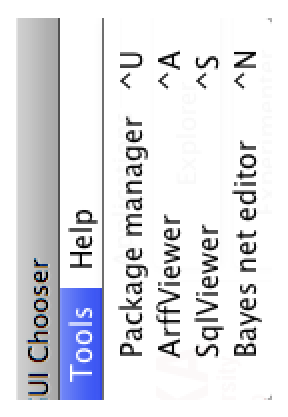
\includegraphics[angle=270,width=2cm]{images/launching/guic_tools.eps}
		\begin{itemize}
			\item \textbf{ArffViewer} An MDI application for viewing ARFF files in spreadsheet format.
			\item \textbf{SqlViewer} Represents an SQL worksheet, for querying databases via JDBC.
                        \item \textbf{Bayes net editor} An application for editing, visualizing and learning Bayes nets.
		\end{itemize}
		
	\item \textbf{Visualization} Ways of visualizing data with WEKA. \\
		\includegraphics[angle=270,width=2cm]{images/launching/guic_visualization.eps}
		\begin{itemize}
			\item \textbf{Plot} For plotting a 2D plot of a dataset.
			\item \textbf{ROC} Displays a previously saved ROC curve.
			\item \textbf{TreeVisualizer} For displaying directed graphs, e.g., a decision tree.
			\item \textbf{GraphVisualizer} Visualizes XML BIF or DOT format graphs, e.g., for Bayesian networks.
			\item \textbf{BoundaryVisualizer} Allows the visualization of classifier decision boundaries in two dimensions.
		\end{itemize}
		
		
	\item \textbf{Help} Online resources for WEKA can be found here. \\
	        \includegraphics[angle=270,width=2cm]{images/launching/guic_help.eps}
		\begin{itemize}
			\item \textbf{Weka homepage} Opens a browser window with WEKA's homepage.
			\item \textbf{HOWTOs, code snippets, etc.} The general WekaWiki \cite{wekawiki}, containing lots of examples and HOWTOs around the development and use of WEKA.
			\item \textbf{Weka on Sourceforge} WEKA's project homepage on Sourceforge.net.
			\item \textbf{SystemInfo} Lists some internals about the Java/WEKA environment, e.g., the \texttt{CLASSPATH}.
		\end{itemize}
\end{enumerate}

To make it easy for the user to add new functionality to the menu without having to modify 
the code of WEKA itself, the GUI now offers a plugin mechanism for such add-ons. 
Due to the inherent dynamic
class discovery, plugins only need to implement the \texttt{weka.gui.MainMenuExtension}
interface and WEKA notified of the package they reside in to be displayed in the menu under 
``Extensions'' (this extra menu appears automatically as soon as extensions are discovered). 
More details can be found in the Wiki article ``Extensions for Weka's main GUI'' 
\cite{mainextensions}.

If you launch WEKA from a terminal window, some text begins scrolling in the
terminal. Ignore this text unless something goes wrong, in which case it can
help in tracking down the cause (the \textit{LogWindow} from the \textit{Program} menu 
displays that information as well).

This User Manual focuses on using the Explorer but does not explain
the individual data preprocessing tools and learning algorithms in
WEKA. For more information on the various filters and learning methods
in WEKA, see the book {\em Data Mining} \cite{witten}.


\chapter{Package Manager}
%
%   This program is free software: you can redistribute it and/or modify
%   it under the terms of the GNU General Public License as published by
%   the Free Software Foundation, either version 3 of the License, or
%   (at your option) any later version.
%
%   This program is distributed in the hope that it will be useful,
%   but WITHOUT ANY WARRANTY; without even the implied warranty of
%   MERCHANTABILITY or FITNESS FOR A PARTICULAR PURPOSE.  See the
%   GNU General Public License for more details.
%
%   You should have received a copy of the GNU General Public License
%   along with this program.  If not, see <http://www.gnu.org/licenses/>.
%

% Version: $Revision: 5897 $


The Package Manager provides a graphical interface to Weka's package
management system. All the functionality available in the command line
client to the package management system covered in the previous
Chapter is available in the GUI version, along with the ability to
install and uninstall multiple packages in one hit.

\section{Main window}

\begin{center}
	\epsfig{file=images/package_manager/manager_main.eps,height=10cm,angle=-90}
\end{center}

The package manager's window is split horizontally into two parts: at
the top is a list of packages and at the bottom is a mini browser that
can be used to display information on the currently selected
package. 

The package list shows the name of a package, its category, the
currently installed version (if installed), the latest version
available via the repository and whether the package has been loaded
or not. This list may be sorted by either package name or category by
clicking on the appropriate column header. A second click on the same
header reverses the sort order. Three radio buttons in the upper left
of the window can be used to filter what is displayed in the list. All
packages (default), all available packages (i.e. those not yet
installed) or only installed packages can be displayed.

If multiple versions of a package are available, they can be accessed by
clicking on an entry in the ``Repository version'' column:

\begin{center}
	\epsfig{file=images/package_manager/manager_versions.eps,height=10cm,angle=-90}
\end{center}

\section{Installing and removing packages}

At the very top of the window are three buttons. On the left-hand side
is a button that can be used to refresh the cached copy of the package
repository meta data. The first time that the package manager (GUI or
command line) is used there will be a short delay as the initial cache
is established. Each time the package manager is used it will check 
with the central repository to see if new packages or updates to 
existing packages are available. If there are updates available, the
user will see a yellow triangular warning icon appear beside the 
``home'' icon under the list of packages. Mousing over this icon will
popup a tooltip showing what updates are available. In order to access
those updates the user must manually refresh the repository cache by 
pressing the ``Refresh repository cache'' button. Following this, the
new/updated packages can be installed as normal.

The two buttons at the top right are used to install and remove
packages repspectively. Multiple packages may be installed/removed by
using a shift-left-click combination to select a range and/or by using
a command-left-click combination to add to the selection. Underneath
the install and uninstall buttons is a checkbox that can be enabled to
ignore any dependencies required by selected packages and any
conflicts that may occur. Installing packages while this checkbox is
selected will \textbf{not} install required dependencies.

Some packages may have additional information on how to complete the
installation or special instructions that gets displayed when the
package is installed:

\begin{center}
	\epsfig{file=images/package_manager/manager_specialInstructions.eps,height=10cm,angle=-90}
\end{center}

Usually it is not necessary to restart Weka after packages have been
installed---the changes should be available immediately. An exception
is when upgrading a package that is already installed. If in doubt, 
restart Weka.

\subsection{Unoffical packages}

The package list shows those packages that have their meta data stored in 
Weka's central meta data repository. These packages are ``official'' Weka 
packages and the Weka team as verified that they appear to provide what is 
advertised (and do not contain malicious code or malware).

It is also possible to install an ``unofficial'' package that has not
gone through the process of become official. Unofficial packages might
be provided, for example, by researchers who want to make experimental
algorithms quickly available to the community for feedback. Unofficial
packages can be installed by clicking the ``File/url'' button on the
top-right of the package manager window. This will bring up an
``Unnoficial package install'' dialog where the user can browse their
file system for a package zip file or directly enter an URL to the
package zip file. Note that no dependency checking is done for
unofficial packages.

\section{Using a http proxy}

Both the GUI and command line package managers can operate via a http proxy. To do so,
start Weka from the command line and supply property values for the proxy host and port:

{\scriptsize
\begin{verbatim}
  java -Dhttp.proxyHost=some.proxy.somewhere.net -Dhttp.proxyPort=port weka.gui.GUIChooser
\end{verbatim}}

If your proxy requires authentication, then two more (non-standard) properties can be
supplied:

{\scriptsize
\begin{verbatim}
  -Dhttp.proxyUser=some_user_name -Dhttp.proxyPassword=some_password
\end{verbatim}}

\section{Using an alternative central package meta data repository}

By default, both the command-line and GUI package managers use the
central package meta data repository hosted on Sourceforge. In the
unlikely event that this site is unavailable for one reason or
another, it is possible to point the package management system at an
alternative repository. This mechanism allows a temporary backup of
the official repostory to be accessed, local mirrors to be established
and alternative repositories to be set up for use etc.

An alternative repository can be specified by setting a Java property:

{\scriptsize
\begin{verbatim}
  weka.core.wekaPackageRepositoryURL=http://some.mirror.somewhere
\end{verbatim}}

This can either be set when starting Weka from the command line with
the \texttt{-D} flag, or it can be placed into a file called
``PackageRepository.props'' in \verb=$WEKA_HOME/props=. The default
value of \verb=WEKA_HOME= is \verb=user.home/wekafiles=, where
\verb=user.home= is the user's home directory. More information on how
and where Weka stores configuration information is given in the
Appendix (Chapter 19).

\section{Package manager property file}

As mentioned in the previous section, an alternative package meta data
repository can be specified by placing an entry in the
PackageRepository.props file in \verb=$WEKA_HOME/props=. From Weka 3.7.8 (and
snapshot builds after 24 September 2012), the package manager also
looks for properties placed in
\verb=$WEKA_HOME/props/PackageManager.props=. The current set of properties
that can be set are:

{\scriptsize
\begin{verbatim}
  weka.core.wekaPackageRepositoryURL=http://some.mirror.somewhere
  weka.packageManager.offline=[true | false]
  weka.packageManager.loadPackages=[true | false]
  weka.pluginManager.disable=com.funky.FunkyExplorerPluginTab
\end{verbatim}}

The default for offline mode (if unspecified) is ``false'' and for
loadPackages is ``true''. \verb=The weka.pluginManager.disable= property can
be used to specify a comma-separated list of fully qualified class
names to ``disable'' in the GUI. This can be used to make problematic
components unavailable in the GUI without having to prevent the entire
package that contains them from being loaded. E.g. ``funkyPackage''
might provide several classifiers and a special Explorer plugin tab
for visualization. Suppose, for example, that the plugin Explorer tab
has issues with certain data sets and causes annoying exceptions to be
generated (or perhaps in the worst cases crashes the Explorer!). In
this case we might want to use the classifiers provided by the package
and just disable the Explorer plugin. Listing the fully qualified name
of the Explorer plugin as a member of the comma-separated list
associated with the \verb=weka.pluginManager.disable= property will achieve
this.


\chapter{Simple CLI}
% Version: $Revision$

The Simple CLI provides full access to all Weka classes, i.e., classifiers, filters, clusterers, etc., but without the hassle of the CLASSPATH (it facilitates the one, with which Weka was started).

It offers a simple \textit{Weka shell} with separated commandline and output.

\begin{center}
	\epsfig{file=images/simplecli/simplecli_main.eps,height=10cm,angle=-90}
\end{center}


\section{Commands}
The following commands are available in the Simple CLI:
\begin{itemize}
	\item \texttt{java <classname> [<args>]} \\
		invokes a java class with the given arguments (if any)
	\item \texttt{break} \\
		stops the current thread, e.g., a running classifier, in a friendly manner
	\item \texttt{kill} \\
		stops the current thread in an unfriendly fashion
	\item \texttt{cls} \\
		clears the output area
	\item \texttt{exit} \\
		exits the Simple CLI
	\item \texttt{help [<command>]} \\
		provides an overview of the available commands if without a command name as argument, otherwise more help on the specified command
\end{itemize}


\section{Invocation}
In order to invoke a Weka class, one has only to prefix the class with "java". This command tells the Simple CLI to load a class and execute it with any given parameters. E.g., the J48 classifier can be invoked on the iris dataset with the following command:
\begin{verbatim}
	java weka.classifiers.trees.J48 -t c:/temp/iris.arff
\end{verbatim}

This results in the following output: 
\begin{center}
	\epsfig{file=images/simplecli/simplecli_j48.eps,height=7cm,angle=-90}
\end{center}


\section{Command redirection}
Starting with this version of Weka one can perform a basic redirection:

\begin{verbatim}
	java weka.classifiers.trees.J48 -t test.arff > j48.txt
\end{verbatim}

\noindent \textbf{Note:} the \texttt{>} must be preceded and followed by a space, otherwise it is not recognized as redirection, but part of another parameter.

\section{Command completion}
Commands starting with java support completion for classnames and filenames via Tab (\texttt{Alt+BackSpace} deletes parts of the command again). In case that there are several matches, Weka lists all possible matches.

\begin{itemize}
	\item \textbf{package name completion}
		\begin{verbatim}
			java weka.cl<Tab>
		\end{verbatim}
		results in the following output of possible matches of package names:
		\begin{verbatim}
			Possible matches:
			  weka.classifiers
			  weka.clusterers
		\end{verbatim}
	\item \textbf{classname completion}
		\begin{verbatim}
			java weka.classifiers.meta.A<Tab>
		\end{verbatim}
		lists the following classes
		\begin{verbatim}
		Possible matches:
		  weka.classifiers.meta.AdaBoostM1
		  weka.classifiers.meta.AdditiveRegression
		  weka.classifiers.meta.AttributeSelectedClassifier
		\end{verbatim}
	\item \textbf{filename completion} \\
	      In order for Weka to determine whether a the string under the cursor is a classname or a filename, filenames need to be absolute (Unix/Linx: \texttt{/some/path/file}; Windows: C:$\backslash$Some$\backslash$Path$\backslash$file) or relative and starting with a dot (Unix/Linux: \texttt{./some/other/path/file}; Windows: .$\backslash$Some$\backslash$Other$\backslash$Path$\backslash$file).
\end{itemize}



\chapter{Explorer}
\begin{figure}[!th]
\centering
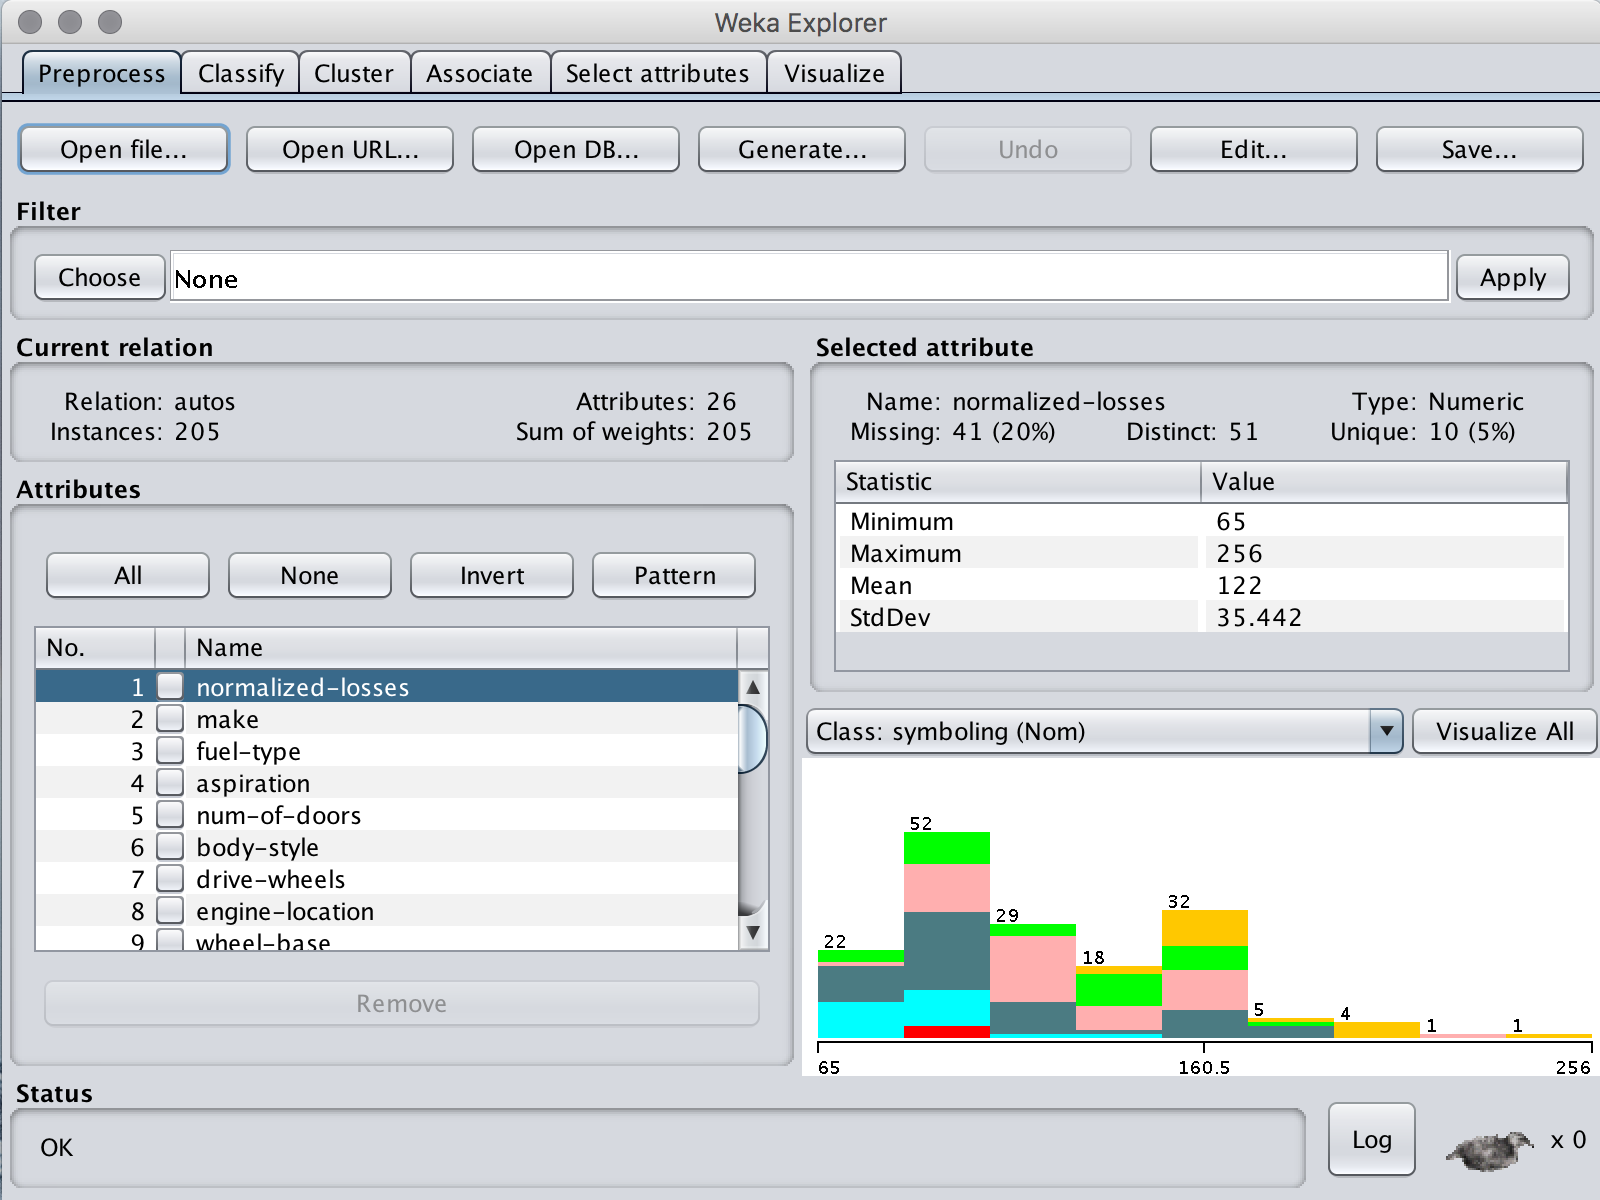
\includegraphics[width=0.9\textwidth]{images/B2_1.png}
\caption{The Explorer interface.}
\label{fig:explorer}
\end{figure}

WEKA's main graphical user interface, the Explorer, gives access to
all its facilities using menu selection and form filling. It is
illustrated in Figure~\ref{fig:explorer}. To begin, there are six
different panels, selected by the tabs at the top, corresponding to
the various data mining tasks that WEKA supports. Further panels can
become available by installing appropriate packages.


\section{Getting started}
\label{sect:getting_started}

Suppose you have some data and you want to build a decision tree from
it. First, you need to prepare the data, then fire up the Explorer and
load in the data. Next you select a decision tree construction method,
build a tree, and interpret the output. It is easy to do it again with
a different tree construction algorithm or a different evaluation
method. In the Explorer you can flip back and forth between the
results you have obtained, evaluate the models that have been built on
different datasets, and visualize graphically both the models and the
datasets themselves---including any classification errors the models
make.

\begin{figure}[!th]
\centering
\subfloat[Spreadsheet.]{\label{subfig:weather_1}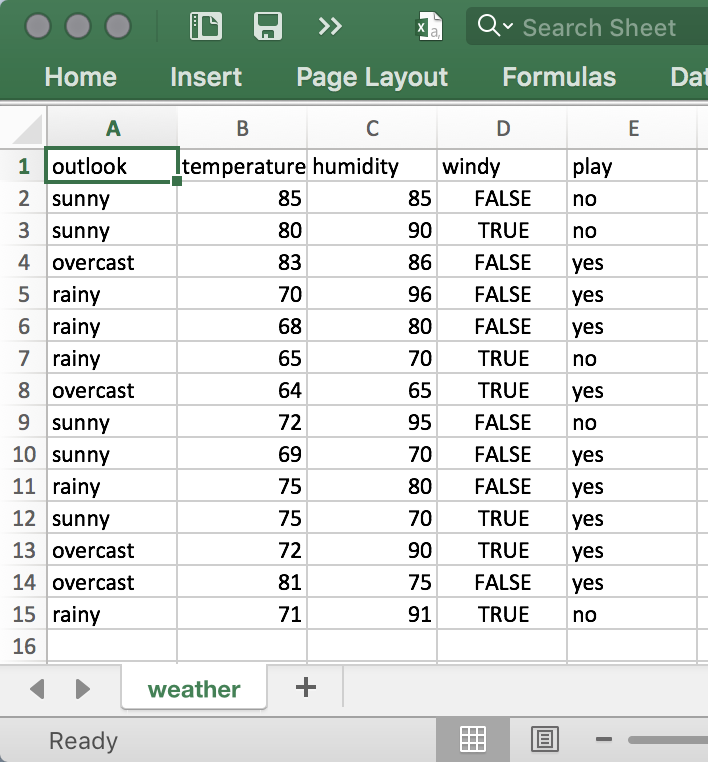
\includegraphics[width=0.45\textwidth]{images/B2_2a.png}}
\qquad
\subfloat[CSV.]{\label{subfig:weather_2}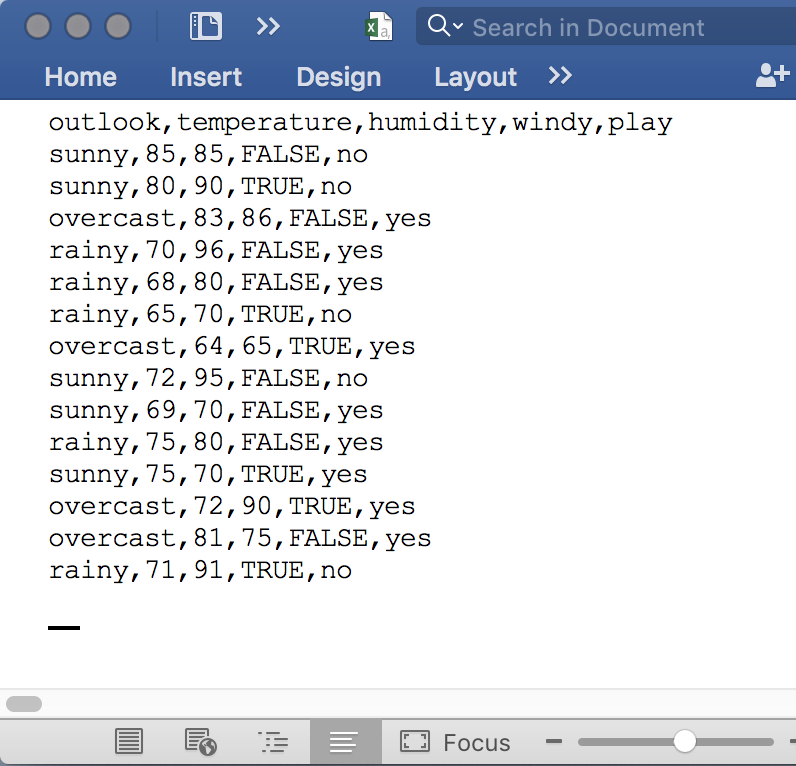
\includegraphics[width=0.45\textwidth]{images/B2_2b.png}}
\newline
\subfloat[ARFF.]{\label{subfig:weather_3}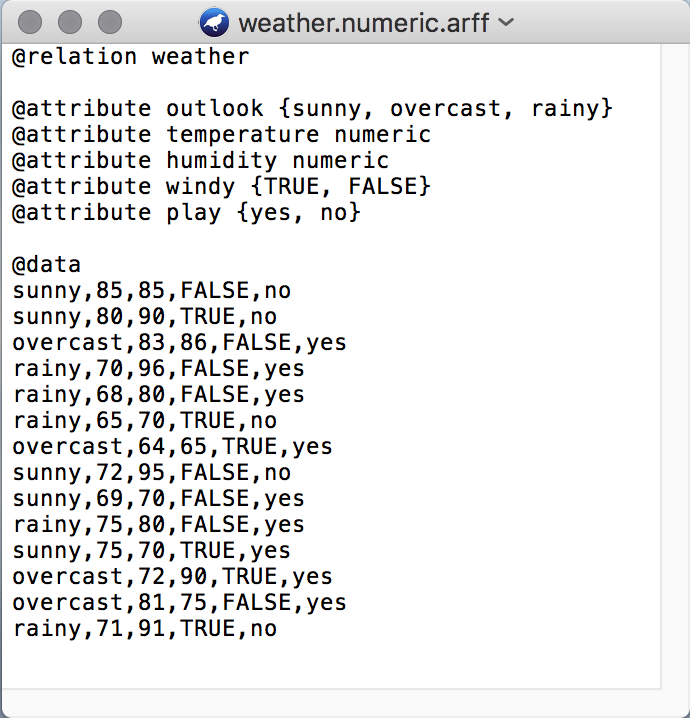
\includegraphics[width=0.45\textwidth]{images/B2_2c.png}}
\caption{\label{fig:weather}Weather data.}
\end{figure}

\subsection{Preparing the data}

The data is often presented in a spreadsheet or database. However,
WEKA's native data storage method is ARFF format. You can easily
convert from a spreadsheet to ARFF. The bulk of an ARFF file consists
of a list of the instances, and the attribute values for each instance
are separated by commas. Most spreadsheet and database programs allow
you to export data into a file in comma-separated value (CSV) format
as a list of records with commas between items. Having done this, you
need only load the file into a text editor or word processor; add the
dataset's name using the @relation tag, the attribute information
using @attribute, and a @data line; and save the file as raw text. For
example, Figure~\ref{fig:weather} shows an Excel spreadsheet
containing the weather data, the data in CSV form loaded into
Microsoft Word, and the result of converting it manually into an ARFF
file. However, you do not actually have to go through these steps to
create the ARFF file yourself, because the Explorer can read CSV
spreadsheet files directly, as described later.

\subsection{Loading the data into the Explorer}

\begin{figure}[!th]
\centering
\subfloat[Choosing the Explorer interface.]{\label{subfig:explorer_1}
\includegraphics[width=0.3\textwidth]{images/B2_3a.png}}
\qquad
\subfloat[Reading in the weather data.]{\label{subfig:explorer_2}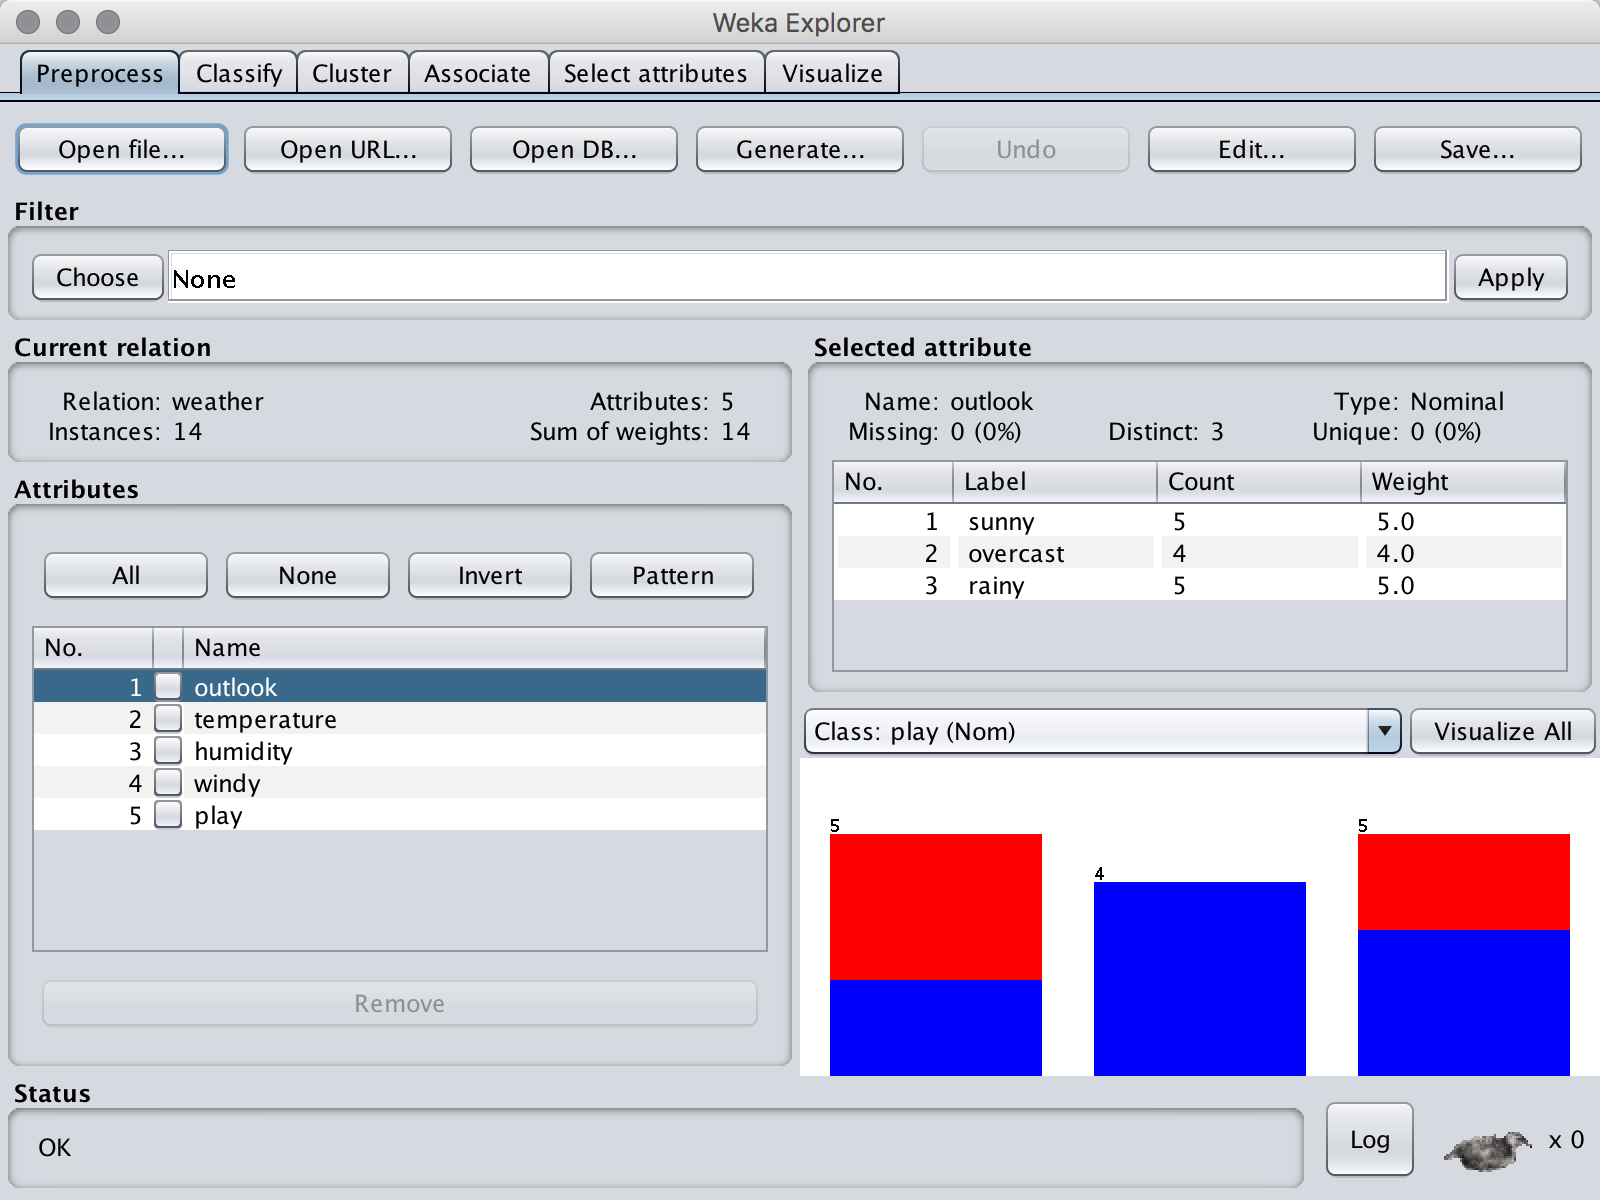
\includegraphics[width=0.6\textwidth]{images/B2_3b.png}}
\caption{\label{fig:weather_explorer}Weather data in the Explorer.}
\end{figure}

Let us load this data into the Explorer and start analyzing it. Fire up
WEKA to get the \textit{GUI Chooser panel} in Figure~\ref{subfig:explorer_1}. Select
\textit{Explorer} from the five choices on the right-hand side. (The
others were mentioned earlier: \textit{Simple CLI} is the
old-fashioned command-line interface.)

What you see next is the main Explorer screen, shown in
Figure~\ref{subfig:explorer_2}. Actually, the figure shows what it will
look like \textit{after} you have loaded in the weather data. The six
tabs along the top are the basic operations that the Explorer
supports: right now we are on \textit{Preprocess}. Click the Open file
button to bring up a standard dialog through which you can select a
file. Choose the \textit{weather.arff} file. If you have it in CSV
format, change from \textit{ARFF data files} to \textit{CSV data
  files}. When you specify a .csv file it is automatically converted
into ARFF format.

Having loaded the file, the screen will be as shown in
Figure~\ref{subfig:explorer_2}. This tells you about the dataset: it
has 14 instances and five attributes (center left); the attributes are
called \textit{outlook}, \textit{temperature}, \textit{humidity},
\textit{windy}, and \textit{play} (lower left). The first attribute,
\textit{outlook}, is selected by default (you can choose others by
clicking them) and has no missing values, three distinct values, and
no unique values; the actual values are \textit{sunny},
\textit{overcast}, and \textit{rainy} and they occur five, four, and
five times, respectively (center right). A histogram at the lower
right shows how often each of the two values of the class,
\textit{play}, occurs for each value of the \textit{outlook}
attribute. The attribute \textit{outlook} is used because it appears
in the box above the histogram, but you can draw a histogram of any
other attribute instead. Here \textit{play} is selected as the class
attribute; it is used to color the histogram, and any filters that
require a class value use it too.

The \textit{outlook} attribute in Figure~\ref{subfig:explorer_2} is
nominal. If you select a numeric attribute, you see its minimum and
maximum values, mean, and standard deviation. In this case the
histogram will show the distribution of the class as a function of
this attribute.

You can delete an attribute by clicking its checkbox and using the
\textit{Remove} button. \textit{All} selects all the attributes,
\textit{None} selects none, Invert \textit{inverts} the current
selection, and \textit{Pattern} selects those attributes whose names
match a user-supplied regular expression. You can undo a change by
clicking the \textit{Undo} button. The \textit{Edit} button brings up
an editor that allows you to inspect the data, search for particular
values and edit them, and delete instances and
attributes. Right-clicking on values and column headers brings up
corresponding context menus.

\subsection{Building a decision tree}
\label{subsection:building_decision_tree}

\begin{figure}[!th]
\centering
\subfloat[Finding J4.8 in the classifiers list.]{\label{subfig:j48_1}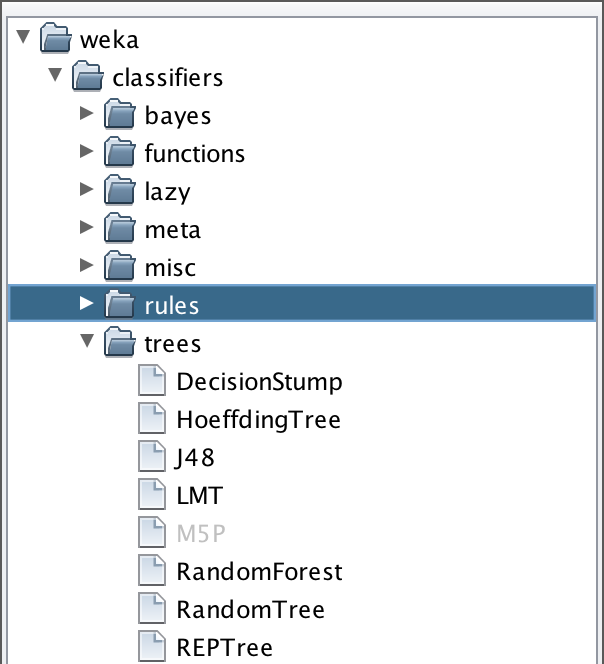
\includegraphics[width=0.3\textwidth]{images/B2_4a.png}}
\qquad
\subfloat[The \textit{Classify} tab.]{\label{subfig:j48_2}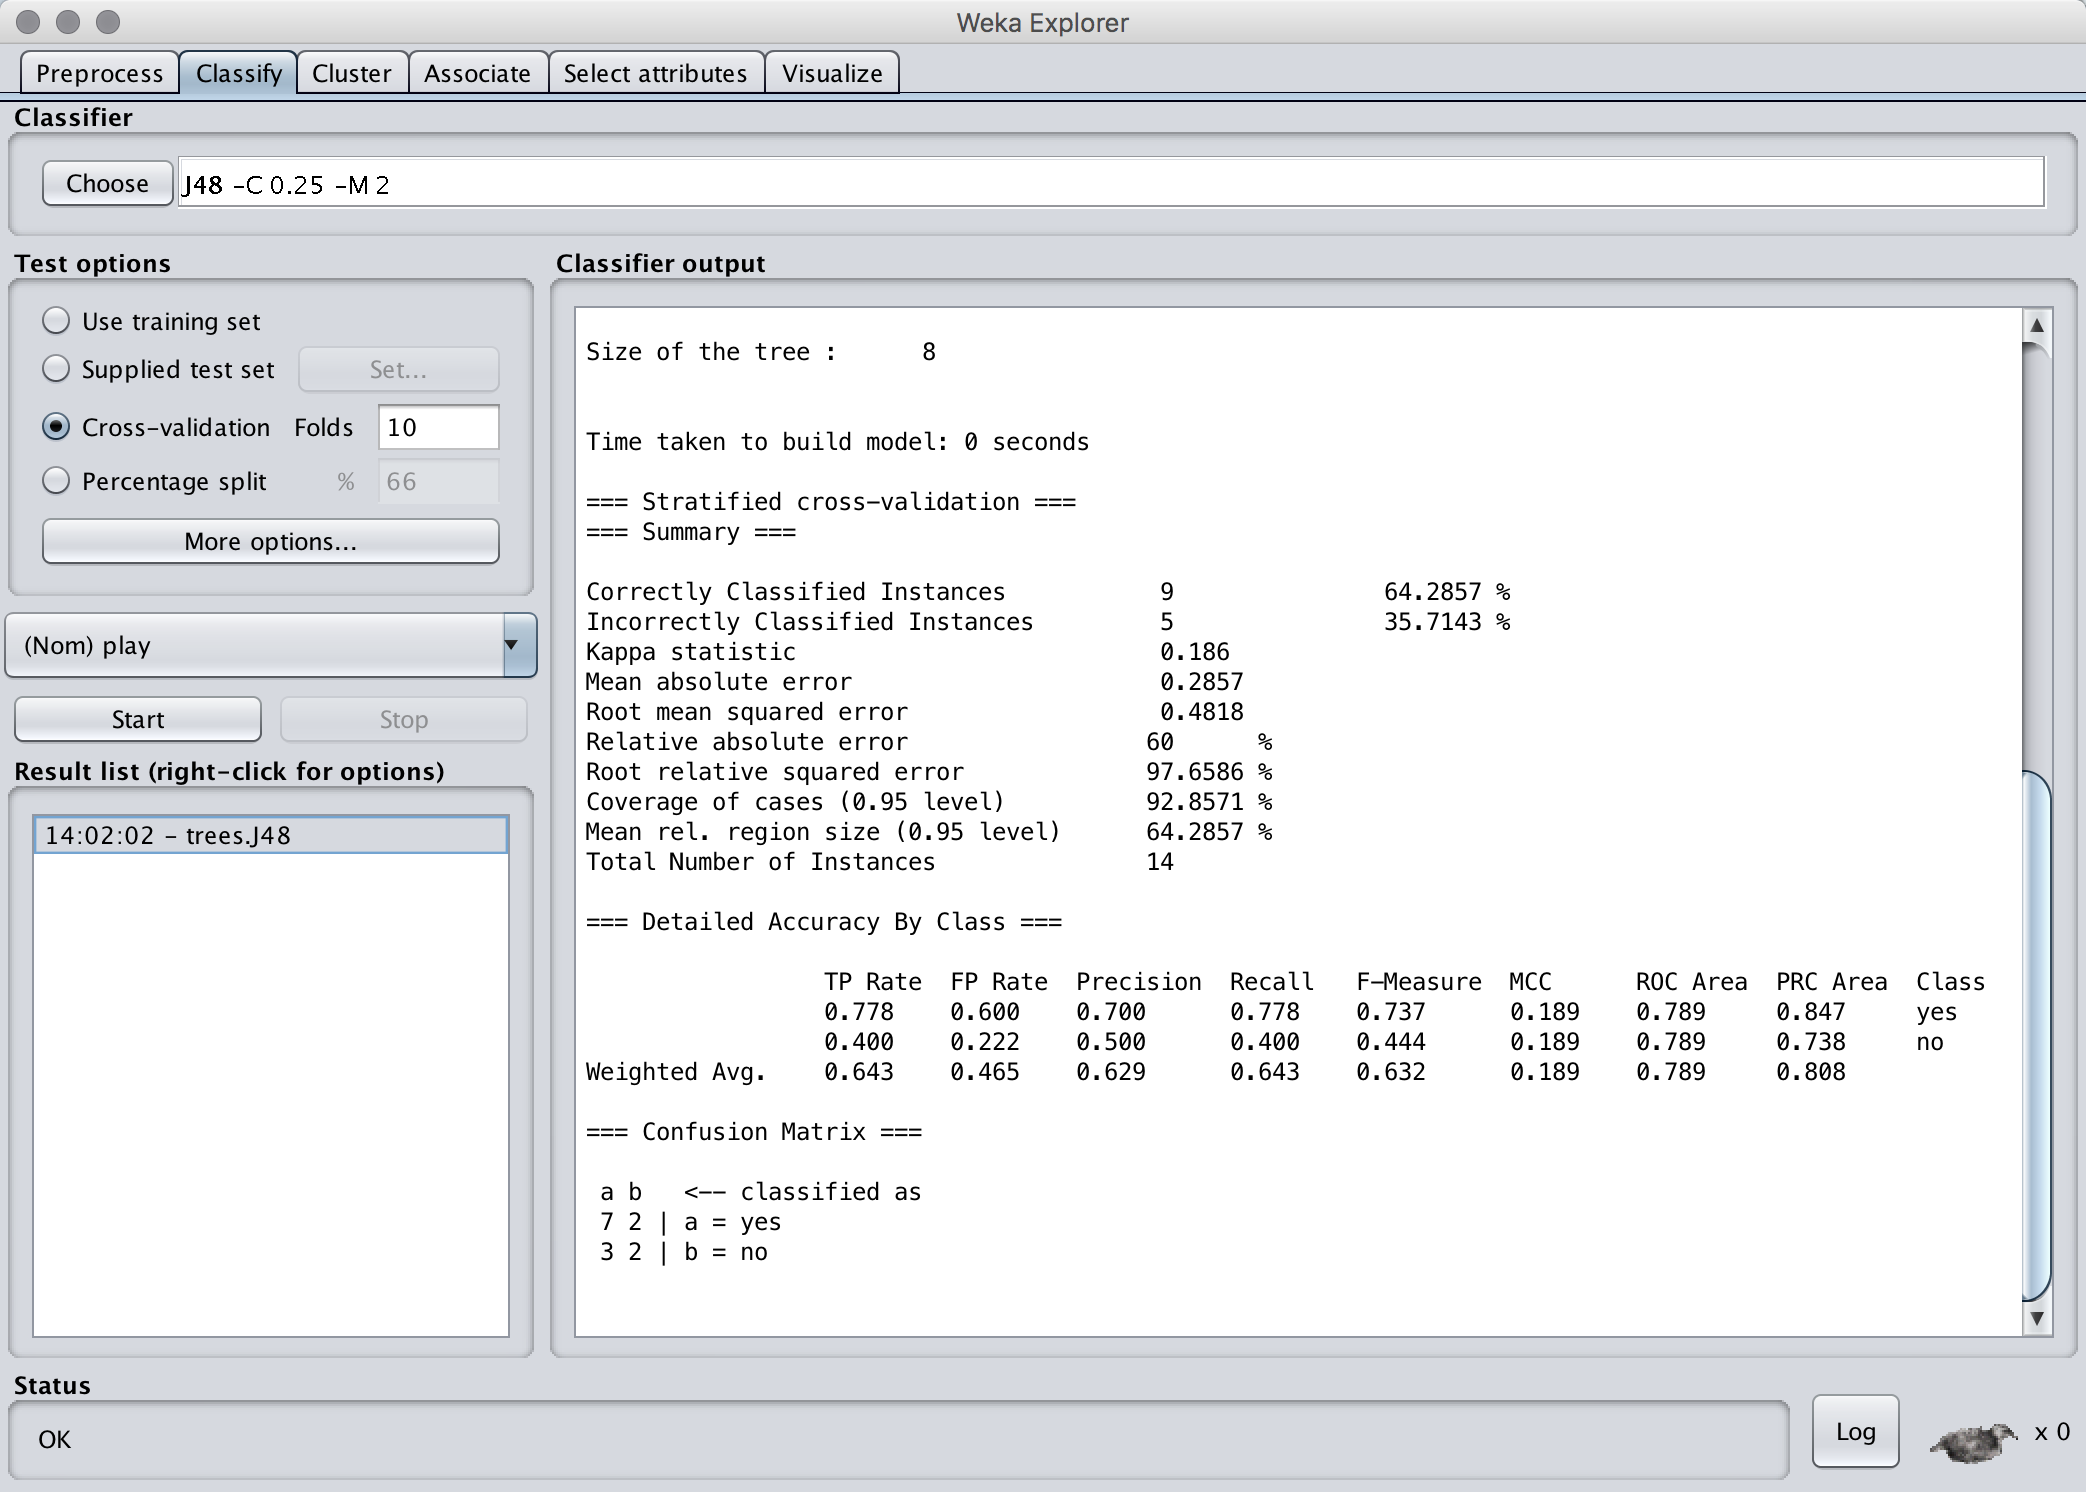
\includegraphics[width=0.6\textwidth]{images/B2_4b.png}}
\caption{\label{fig:j48_explorer}J4.8 in the Explorer.}
\end{figure}

To see what the C4.5 decision tree learner does with this dataset, use
the J4.8 algorithm, which is WEKA's implementation of this
algorithm. (J4.8 actually implements a later and slightly improved
version called C4.5 revision 8, which was the last public version of
this family of algorithms before C5.0 was released.) Click the
\textit{Classify} tab to get a screen that looks like
Figure~\ref{subfig:j48_2}. Actually, the figure shows what it will
look like \textit{after} you have analyzed the weather data.

First select the classifier by clicking the \textit{Choose} button at
the top left, opening up the trees section of the hierarchical menu in
Figure~\ref{subfig:j48_1}, and finding \textit{J48}. The menu
structure represents the organization of the WEKA code into modules
and the items you need to select are always at the lowest level. Once
selected, \textit{J48} appears in the line beside the \textit{Choose}
button as shown in Figure~\ref{subfig:j48_2}, along with its default parameter
values. If you click that line, the J4.8 classifier's object editor
opens up and you can see what the parameters mean and alter their
values if you wish. The Explorer generally chooses sensible defaults.

Having chosen the classifier, invoke it by clicking the \textit{Start}
button. WEKA works for a brief period---when it is working, the little
bird at the lower right of Figure 2.4b jumps up and dances---and then
produces the output shown in the main panel of
Figure~\ref{subfig:j48_2}.

\subsection{Examining the output}

\begin{figure}[!th]
%\centering
\begin{mdframed}[innermargin=-1cm]
\begin{Verbatim}[fontsize=\footnotesize]
=== Run information ===

Scheme:       weka.classifiers.trees.J48 -C 0.25 -M 2
Relation:     weather
Instances:    14
Attributes:   5
              outlook
              temperature
              humidity
              windy
              play
Test mode:    10-fold cross-validation

=== Classifier model (full training set) ===

J48 pruned tree
------------------

outlook = sunny
|   humidity <= 75: yes (2.0)
|   humidity > 75: no (3.0)
outlook = overcast: yes (4.0)
outlook = rainy
|   windy = TRUE: no (2.0)
|   windy = FALSE: yes (3.0)

Number of Leaves  : 5

Size of the tree : 8

Time taken to build model: 0.27 seconds

=== Stratified cross-validation ===
=== Summary ===

Correctly Classified Instances           9               64.2857 %
Incorrectly Classified Instances         5               35.7143 %
Kappa statistic                          0.186 
Mean absolute error                      0.2857
Root mean squared error                  0.4818
Relative absolute error                 60      %
Root relative squared error             97.6586 %
Total Number of Instances               14     

=== Detailed Accuracy By Class ===

               TP Rate   FP Rate   Precision   Recall  F-Measure   ROC Area  Class
                 0.778     0.6        0.7       0.778     0.737      0.789    yes
                 0.4       0.222      0.5       0.4       0.444      0.789    no
Weighted Avg.    0.643     0.465      0.629     0.643     0.632      0.789

=== Confusion Matrix ===

 a b   <-- classified as
 7 2 | a = yes
 3 2 | b = no
\end{Verbatim}
\end{mdframed}
\caption{\label{fig:j48_output}Output from the J4.8 decision tree learner.}
\end{figure}

Figure 2.5 shows the full output (Figure~\ref{subfig:j48_2} only gives
the lower half). At the beginning is a summary of the dataset, and the
fact that 10-fold cross-validation was used to evaluate it. That is
the default, and if you look closely at Figure~\ref{subfig:j48_2} you
will see that the \textit{Cross-validation} box at the left is
checked. Then comes a pruned decision tree in textual form. The model
that is shown here is always one generated from the full dataset
available from the \textit{Preprocess panel}. The first split is on
the outlook attribute, and then, at the second level, the splits are
on humidity and windy, respectively. In the tree structure, a colon
introduces the class label that has been assigned to a particular
leaf, followed by the number of instances that reach that leaf,
expressed as a decimal number because of the way the algorithm uses
fractional instances to handle missing values. If there were
incorrectly classified instances (there aren't in this example) their
number would appear too: thus \textit{2.0/1.0} means that two
instances reached that leaf, of which one is classified
incorrectly. Beneath the tree structure the number of leaves is
printed; then the total number of nodes (\textit{Size of the
  tree}). There is a way to view decision trees more graphically,
which we will encounter later.

%% Fix the reference above to page 484

The next part of the output gives estimates of the tree's predictive
performance. In this case they are obtained using stratified
cross-validation with 10 folds, the default in
Figure~\ref{subfig:j48_2}. As you can see, more than 30\% of the
instances (5 out of 14) have been misclassified in the
cross-validation. This indicates that the results obtained from the
training data are optimistic compared with what might be obtained from
an independent test set from the same source. From the confusion
matrix at the end observe that 2 instances of class \textit{yes} have
been assigned to class \textit{no} and 3 of class \textit{no} are
assigned to class \textit{yes}.

As well as the classification error, the evaluation module also
outputs the Kappa statistic, the mean absolute error, and the root
mean-squared error of the class probability estimates assigned by the
tree. The root mean-squared error is the square root of the average
squared loss. The mean absolute error is calculated in a similar way
using the absolute instead of the squared difference. It also outputs
relative errors, which are based on the prior probabilities (i.e.,
those obtained by the ZeroR learning scheme described later). Finally,
for each class it also outputs various statistics. Also reported is
the per-class average of each statistic, weighted by the number of
instances from each class. All of these evaluation measures are
discussed in Chapter 5 of the book.

\subsection{Doing it again}
\label{subsec:doing_it_again}

You can easily run J4.8 again with a different evaluation
method. Select {\em Use training set} (near the top left in
Figure~\ref{subfig:j48_2}) and click \textit{Start} again. The
classifier output is quickly replaced to show how well the derived
model performs on the training set, instead of showing the
cross-validation results. This evaluation is highly optimistic. It may
still be useful, because it generally represents an upper bound to the
model's performance on fresh data. In this case, all 14 training
instances are classified correctly. In some cases a classifier may
decide to leave some instances unclassified, in which case these will
be listed as \textit{Unclassified Instances}. This does not happen for
most learning schemes in WEKA.

The panel in Figure~\ref{subfig:j48_2} has further test options:
\textit{Supplied test set}, in which you specify a separate file
containing the test set, and \textit{Percentage split}, with which you
can hold out a certain percentage of the data for testing. You can
output the predictions for each instance by clicking the \textit{More
  options} button and checking the appropriate entry. There are other
useful options, such as suppressing some output and including other
statistics such as entropy evaluation measures and cost-sensitive
evaluation. For the latter you must enter a cost matrix: type the
number of classes into the \textit{Classes} box (and terminate it with
the \textit{Enter} or \textit{Return} key) to get a default cost
matrix, then edit the values as required.

\subsection{Working with models}

The small pane at the lower left of Figure~\ref{subfig:j48_2}, which
contains one highlighted line, is a history list of the results. The
Explorer adds a new line whenever you run a classifier. Because you
have now run the classifier twice, the list will contain two items. To
return to a previous result set, click the corresponding line and the
output for that run will appear in the Classifier Output pane. This
makes it easy to explore different classifiers or evaluation schemes
and revisit the results to compare them.

The result history list is the entry point to some powerful features
of the Explorer. When you \textit{right}-click an entry a menu appears that
allows you to view the results in a separate window, or save the
result buffer. More importantly, you can save the model that WEKA has
generated in the form of a Java object file. You can reload a model
that was saved previously, which generates a new entry in the result
list. If you now supply a test set, you can reevaluate the old model
on that new set.

Several items on the right-click menu allow you to visualize the
results in various ways. At the top of the Explorer interface is a
separate \textit{Visualize} tab, but that is different: it shows the
dataset, not the results for a particular model. By right-clicking an
entry in the history list you can see the classifier errors. If the
model is a tree or a Bayesian network you can see its structure. You
can also view the margin curve and various cost and threshold curves,
including the cost/benefit analysis tool. For all of these you must
choose a class value from a submenu. The \textit{Visualize threshold
  curve} menu item allows you to see the effect of varying the
probability threshold above which an instance is assigned to that
class. You can select from a wide variety of curves that include the
ROC and recall-precision curves. To see these, choose the X- and
Y-axes appropriately from the menus given. For example, set X to
\textit{False Positive Rate} and Y to \textit{True Positive Rate} for
an ROC curve or X to \textit{Recall} and Y to \textit{Precision} for a
recall-precision curve.

\begin{figure}[!th]
\centering
\subfloat[\textit{J4.8} tree for the iris data.]{\label{subfig:j48_3}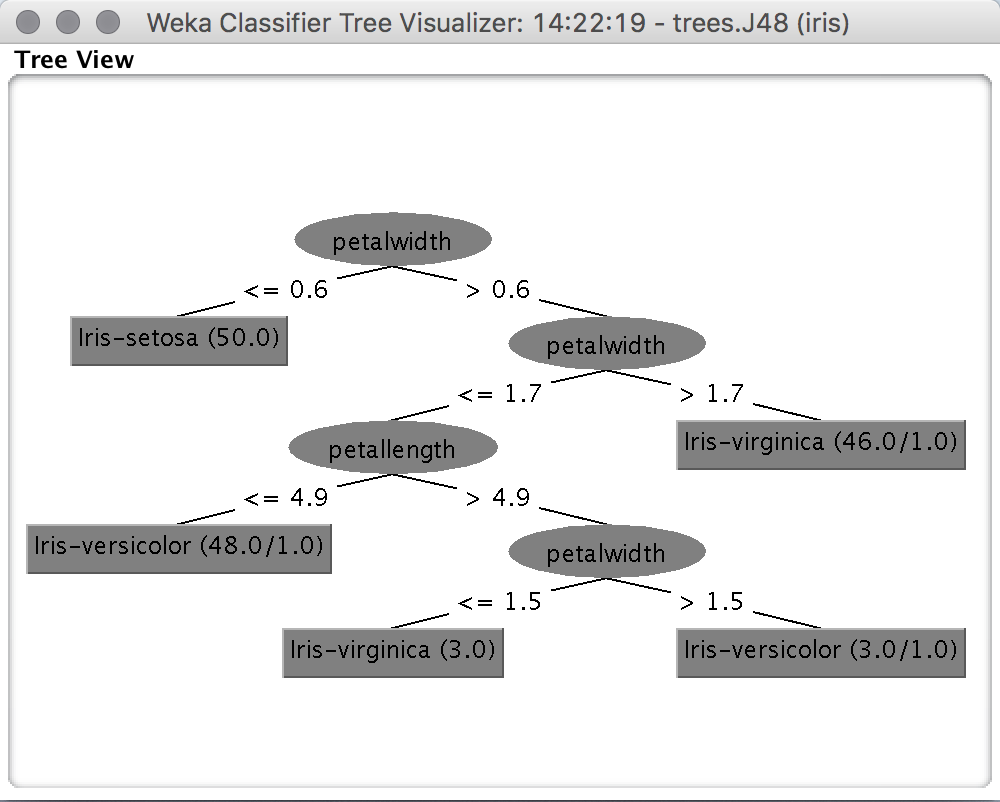
\includegraphics[width=0.9\textwidth]{images/B2_6a.png}}
\newline
\subfloat[\textit{J4.8}'s errors on the iris data.]{\label{subfig:j48_4}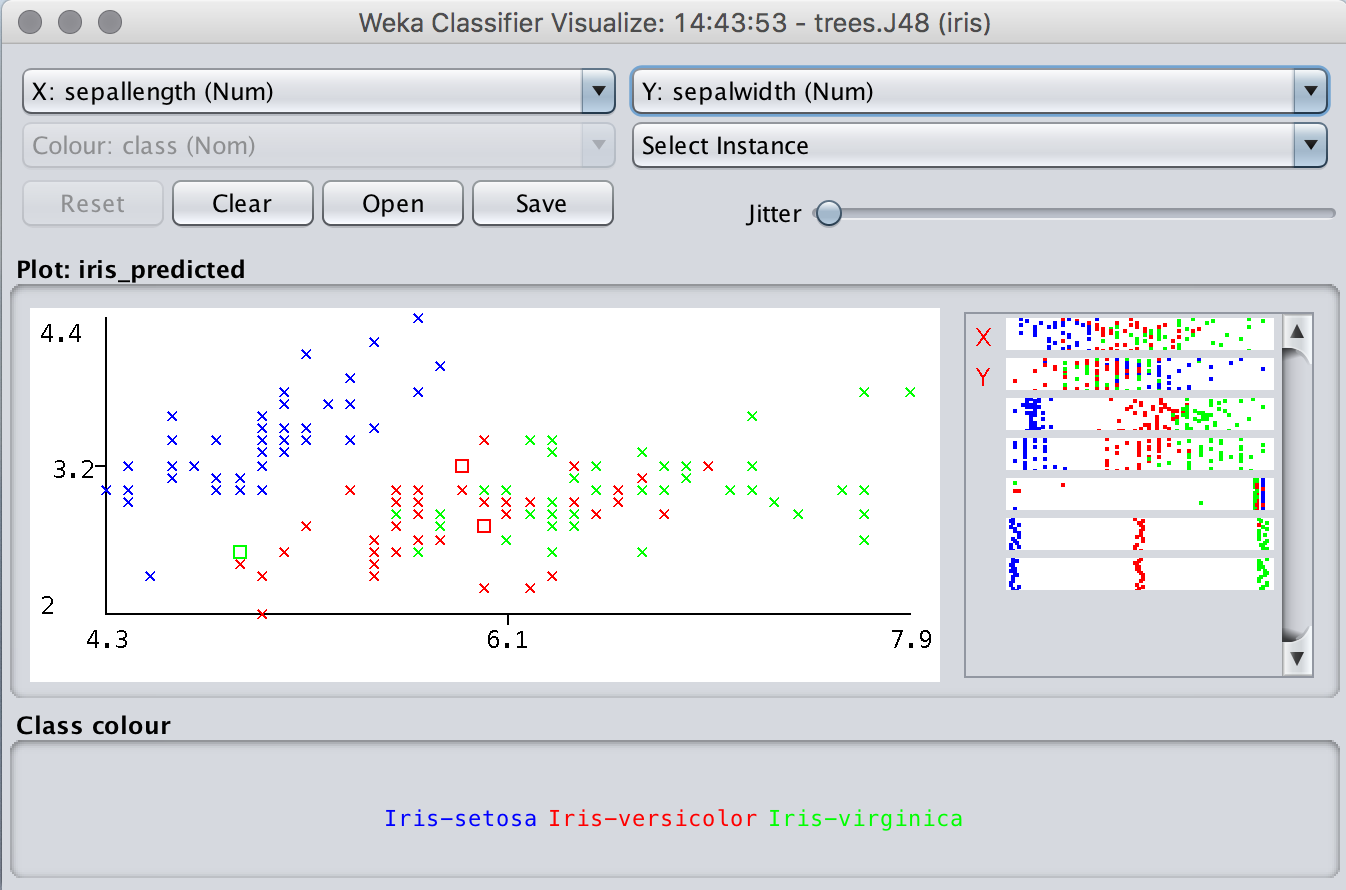
\includegraphics[width=0.9\textwidth]{images/B2_6b.png}}
\caption{\label{fig:j48_iris}Visualizing the result of \textit{J4.8} on the iris data.}
\end{figure}

Figure~\ref{fig:j48_iris} shows two ways of looking at the result of
using J4.8 to classify the iris dataset---we use this rather than the
weather data because it produces more interesting
pictures. Figure~\ref{subfig:j48_3} shows the tree. Right-click a
blank space in this window to bring up a menu enabling you to
automatically scale the view or force the tree into the window. Drag
the mouse to pan around the space. It's also possible to visualize the
instance data at any node, if it has been saved by the learning
algorithm.

Figure~\ref{subfig:j48_4} shows the classifier errors on a
two-dimensional plot. You can choose which attributes to use for X and
Y using the selection boxes at the top. Alternatively, click one of
the speckled horizontal strips to the right of the plot: left-click
for X and right-click for Y. Each strip shows the spread of instances
along that attribute. X and Y appear beside the ones you have chosen
for the axes.

The data points are colored according to their class: blue, red and
green for \textit{Iris setosa}, \textit{Iris versicolor}, and
\textit{Iris virginica}, respectively (there is a key at the bottom of
the screen). Correctly classified instances are shown as crosses;
incorrectly classified ones appear as boxes (of which there are three
in Figure~\ref{subfig:j48_4}). You can click on an instance to bring
up relevant details: its instance number, the values of the
attributes, its class, and the predicted class.

\subsection{When things go wrong}

Beneath the result history list, at the bottom of
Figure~\ref{subfig:explorer_2}, is a status line that says, simply,
\textit{OK}. Occasionally this changes to \textit{See error log}, an
indication that something has gone wrong. For example, there may be
constraints among the various different selections you can make in a
panel. Most of the time the interface grays out inappropriate
selections and refuses to let you choose them. But occasionally the
interactions are more complex, and you can end up selecting an
incompatible set of options. In this case, the status line changes
when WEKA discovers the incompatibility---typically when you press
\textit{Start}. To see the error, click the \textit{Log} button to the
left of the bird in the lower right-hand corner of the interface. WEKA
also writes a detailed log to a file, called \textit{weka.log}, under
the \textit{wekafiles} directory in the user's home directory. This
often contains more information about the causes of problems than the
Explorer's Log window because it captures debugging output directed to
the standard out and error channels.

\section{Exploring the Explorer}
\label{section:exploring_the_explorer}

We have briefly investigated two of the six tabs at the top of the
Explorer window in Figure~\ref{subfig:explorer_2} and
Figure~\ref{subfig:j48_2}. In summary, here's what all of the tabs do:

\begin{enumerate}
\item \textit{Preprocess}: Choose the dataset and modify it in various ways.
\item \textit{Classify}: Train learning schemes that perform classification or regression and evaluate them.
\item \textit{Cluster}: Learn clusters from the dataset.
\item \textit{Associate}: Learn association rules for the data and evaluate them.
\item \textit{Select attributes}: Select the most relevant aspects of the dataset.
\item \textit{Visualize}: View different two-dimensional plots of the data and interact with them.
\end{enumerate}

Each tab gives access to a whole range of facilities. In our tour so
far, we have barely scratched the surface of the \textit{Preprocess}
and \textit{Classify} panels.

At the bottom of every panel is a \textit{Status} box and a
\textit{Log} button. The status box displays messages that keep you
informed about what's going on. For example, if the Explorer is busy
loading a file, the status box will say so. Right-clicking anywhere
inside this box brings up a little menu with two options: display the
amount of memory available to WEKA, and run the Java garbage
collector. Note that the garbage collector runs constantly as a
background task anyway.

Clicking the \textit{Log} button opens a textual log of the actions that WEKA
has performed in this session, with timestamps.

As noted earlier, the little bird at the lower right of the window
jumps up and dances when WEKA is active. The number beside the $\times$
shows how many concurrent processes are running. If the bird is
standing but stops moving, it's sick! Something has gone wrong, and
you may have to restart the Explorer.

\subsection{Loading and filtering files}

Along the top of the \textit{Preprocess panel} in
Figure~\ref{subfig:explorer_2} are buttons for opening files, URLs,
and databases. Initially, only files whose names end in \textit{.arff}
appear in the file browser; to see others, change the \textit{Format}
item in the file selection box.

\subsection{Converting files to ARFF}

WEKA has converters for the following file formats: 

\begin{itemize}
\item spreadsheet files with extension \textit{.csv},
\item C4.5's native file format with extensions \textit{.names} and \textit{.data},
\item serialized instances with extension \textit{.bsi},
\item LIBSVM format files with extension \textit{.libsvm},
\item SVM-Light format files with extension \textit{.dat},
\item XML-based ARFF format files with extension \textit{.xrff},
\item JSON-based ARFF format files with extension \textit{.json},
\item ASCII Matlab files with extension \textit{.m}.
\end{itemize}

\begin{figure}[!th]
\centering
\subfloat[Generic Object Editor.]{\label{subfig:goe_1}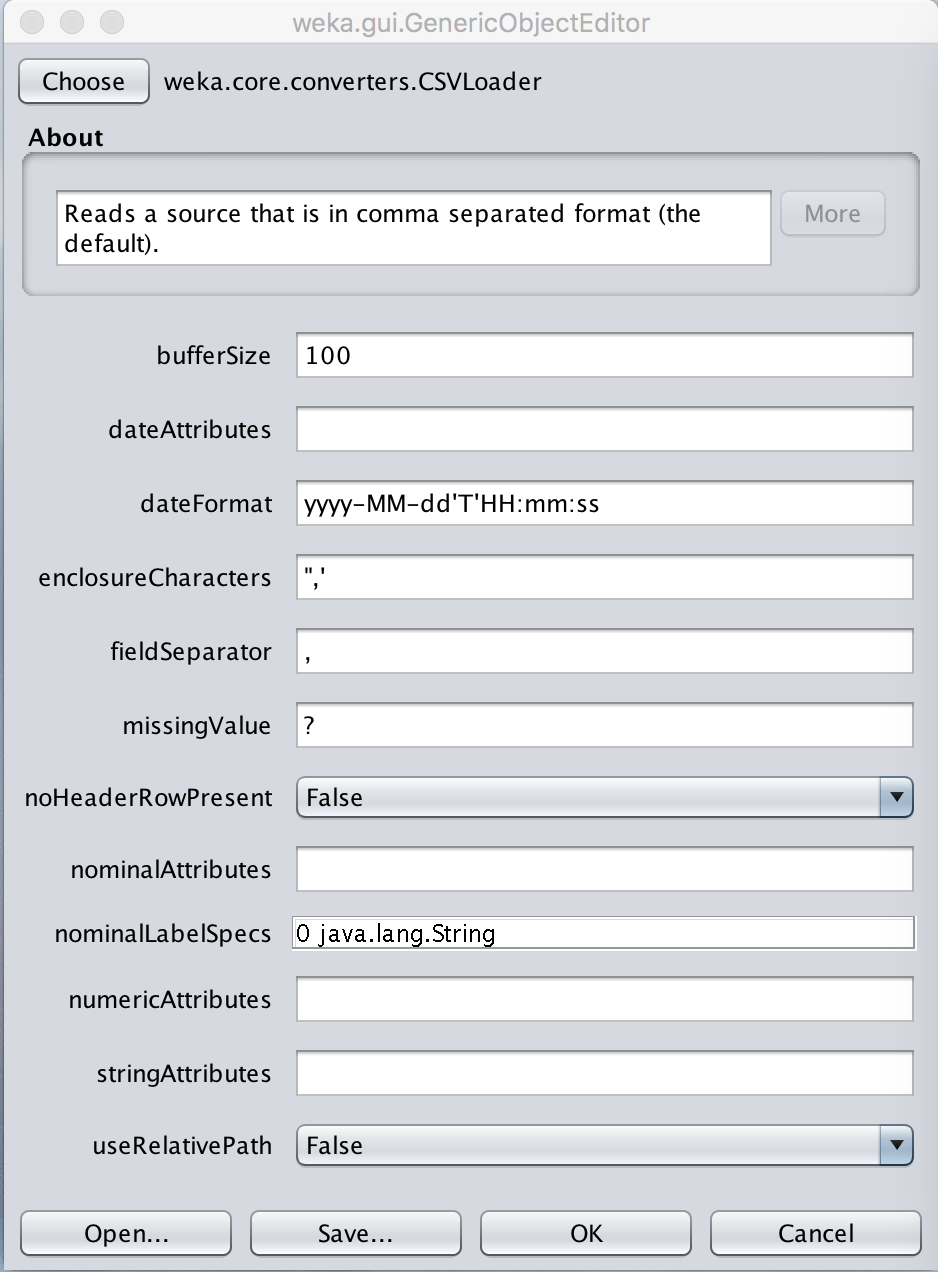
\includegraphics[width=0.45\textwidth]{images/B2_7a.png}}
\qquad
\subfloat[More information.]{\label{subfig:goe_2}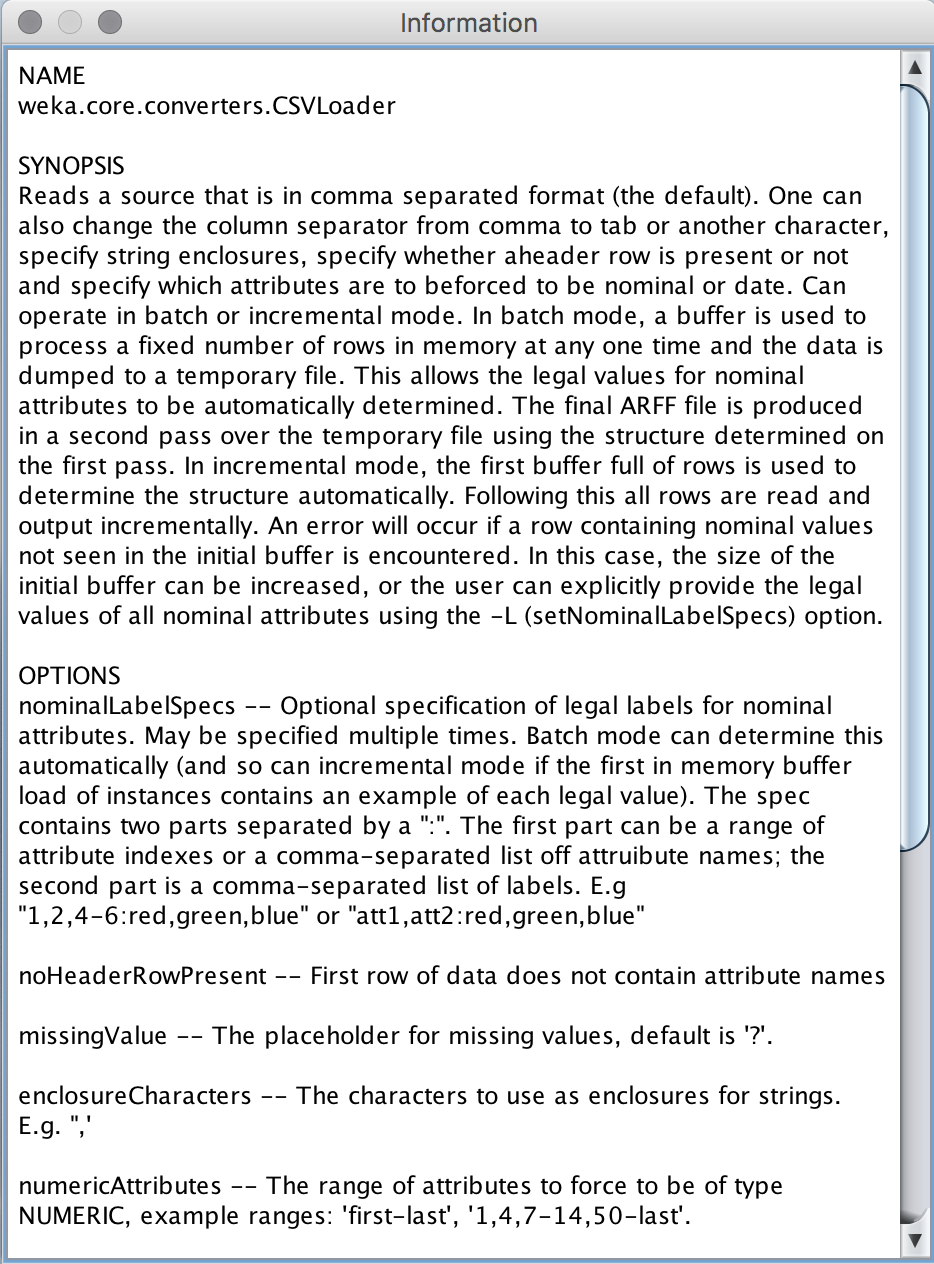
\includegraphics[width=0.45\textwidth]{images/B2_7b.png}}
\newline
\subfloat[Choosing a converter (click Choose).]{\label{subfig:goe_3}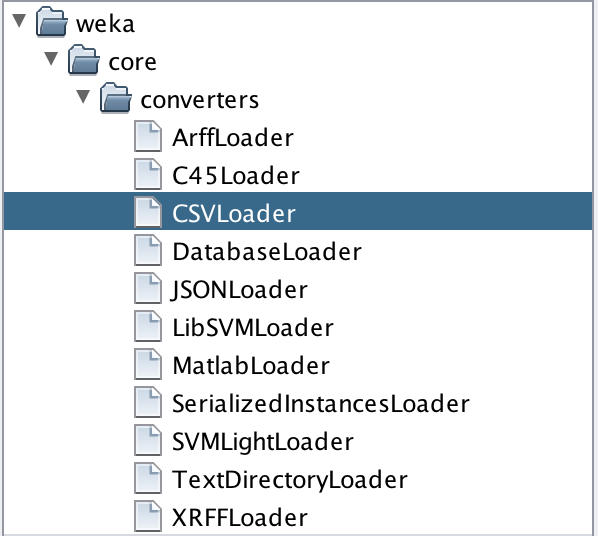
\includegraphics[width=0.45\textwidth]{images/B2_7c.png}}
\caption{\label{fig:goe}The Generic Object Editor.}
\end{figure}

The appropriate converter is used based on the file extension. If WEKA
cannot load the data, it tries to interpret it as ARFF. If that fails,
it pops up the box shown in Figure~\ref{subfig:goe_1}.

This is a generic object editor, used throughout WEKA for selecting
and configuring object. For example, when you set parameters for a
classifier, you use the same kind of box. The \textit{CSVLoader} for
\textit{.csv} files is selected by default, and the \textit{More}
button gives you more information about it, shown in
Figure~\ref{subfig:goe_2}. It is always worth looking at the
documentation! In this case, it explains that the spreadsheet's first
row determines the attribute names and gives a brief description of
the CSVLoader's options. Click \textit{OK} to use this converter. For
a different one, click \textit{Choose} to select from the list in
Figure~\ref{subfig:goe_3}.

\begin{figure}[!th]
\centering
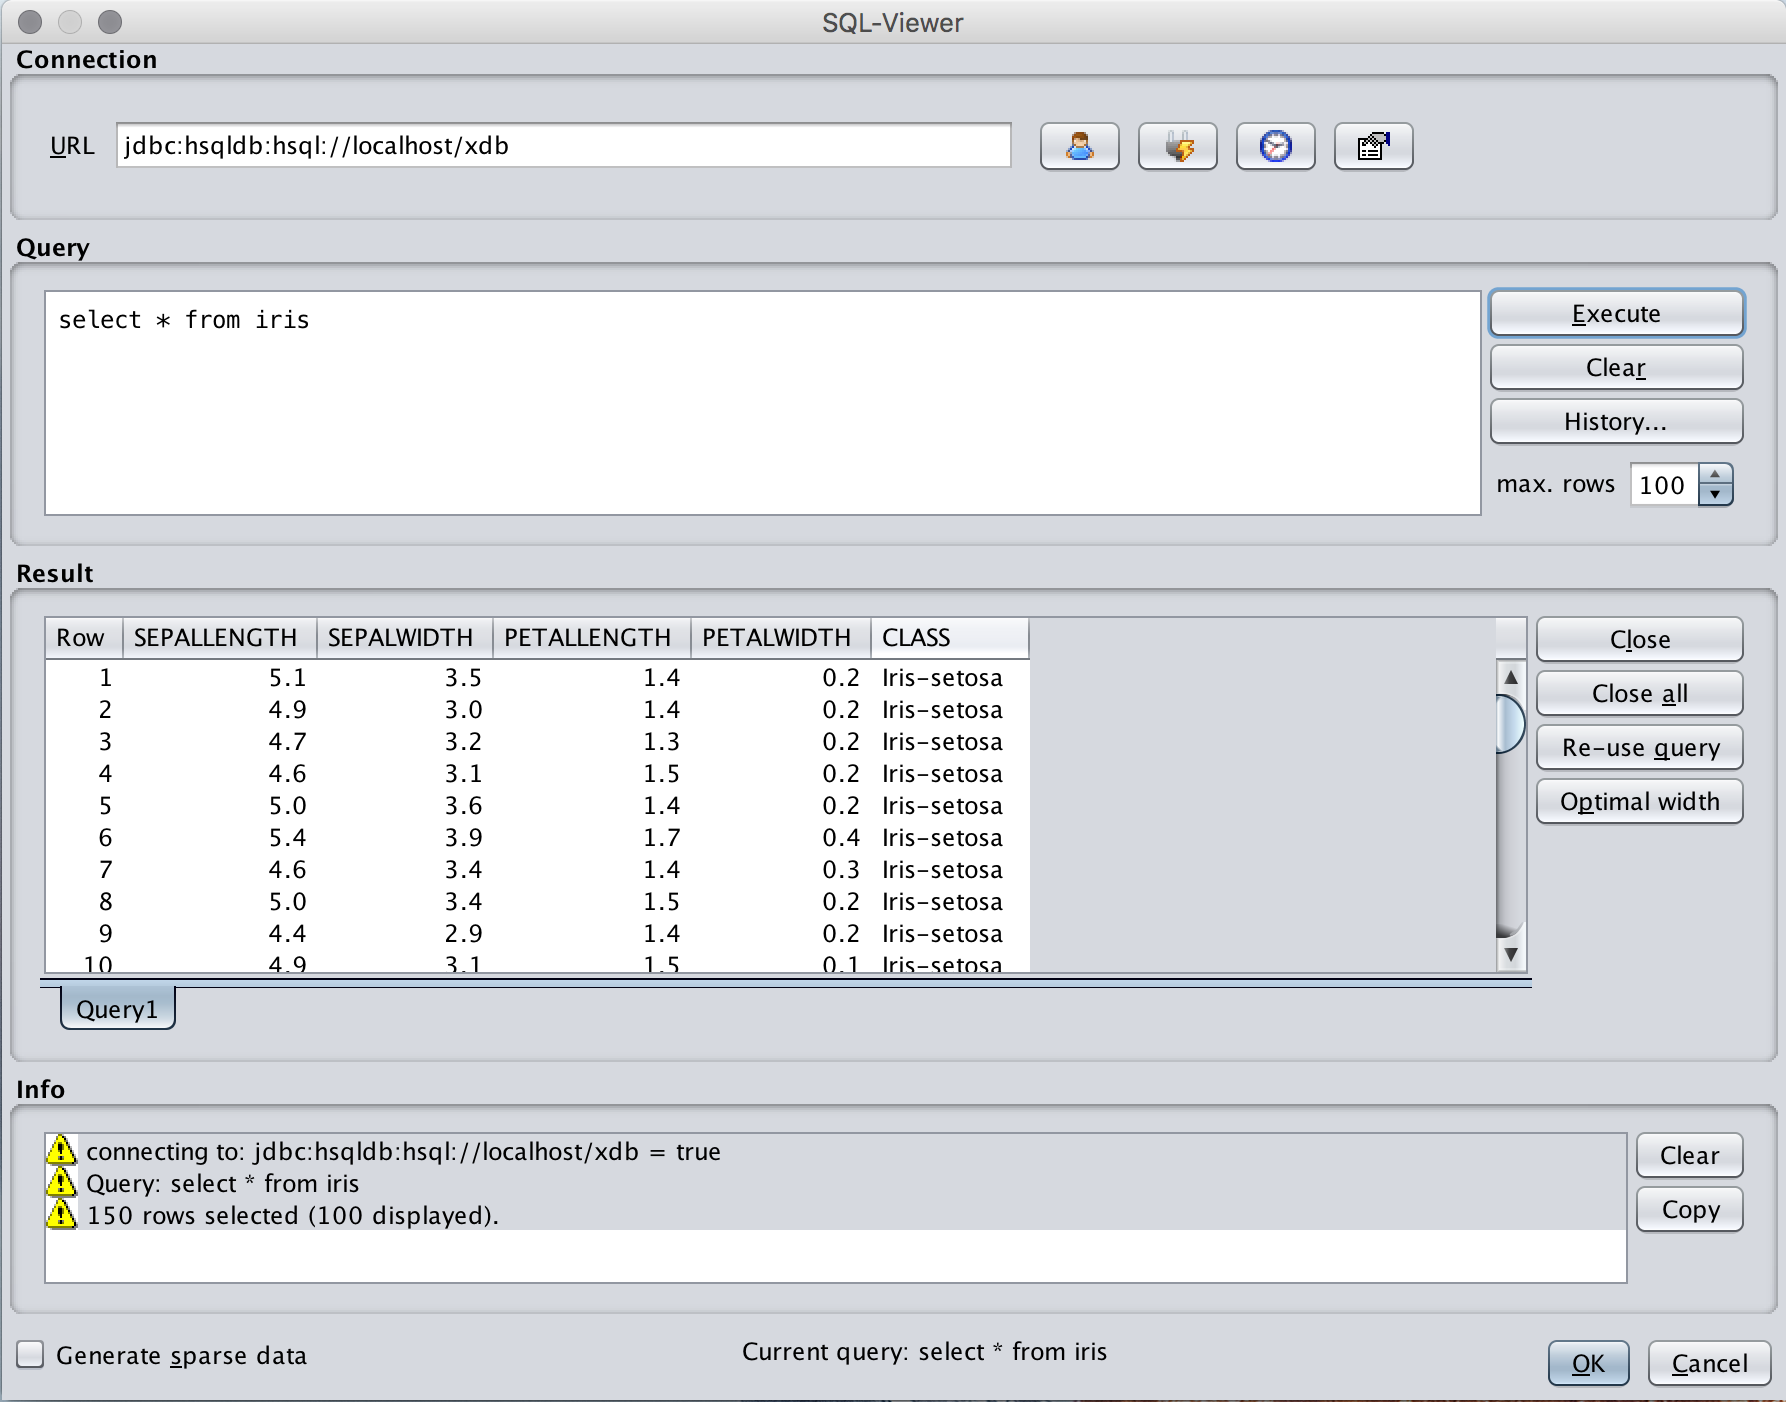
\includegraphics[width=0.9\textwidth]{images/B2_8.png}
\caption{The SQLViewer tool.}
\label{fig:sql_viewer}
\end{figure}


The \textit{ArffLoader} is the first option, and we reached this point
only because it failed. The second option is for the C4.5 format, in
which there are two files for a dataset, one giving field names and
the other giving the actual data. The third option,
\textit{CSVLoader}, is the default, and we clicked \textit{Choose}
because we want a different one. The fourth option is for reading from
a database rather than a file; however, the \textit{SQLViewer} tool,
shown in Figure~\ref{fig:sql_viewer} and accessible by pressing the \textit{Open DB}
button on the \textit{Preprocess} panel, is a more user-friendly route
for accessing a database. The ``serialized instances'' option is for
reloading datasets that have been saved as Java serialized object. Any
Java object can be saved in this format and reloaded. As a native Java
format, it is quicker to load that an ARFF file, which must be parsed
and checked. When repeatedly reloading a large dataset it may be worth
saving it in this form.

The tenth menu item is for importing a directory containing plain text
files for the purposes of text mining. The imported directory is
expected to have a specific structure---namely a set of
subdirectories, each containing one or more text files with the
extension \textit{.txt}. Each text file becomes one instance in the
dataset, with a string attribute holding the contents of the file and
a nominal class attribute holding the name of the subdirectory that it
came from. This dataset can then be further processed into word
frequencies using the \textit{StringToWordVector} filter (covered in
the next section). The last option is for loading data files in XRFF,
the XML Attribute Relation File format. As the name suggests, this
gives ARFF header and instance information in the XML markup language.

Further features of the generic object editor in Figure~\ref{subfig:goe_1} are
\textit{Save}, which saves a configured object, and \textit{Open},
which opens a previously saved one. These are not useful for this
particular kind of object. But other generic object editor panels have
many editable properties, and having gone to some trouble to set them
up you may want to save the configured object to reuse later.

Files on your computer are not the only source of datasets for
WEKA. You can open a URL, and WEKA will use the hypertext transfer
protocol (HTTP) to download an ARFF file from the Web. Or you can open
a database (Open DB)---any database that has a Java database
connectivity (JDBC) driver---and retrieve instances using the SQL
\textit{Select} statement. This returns a relation that WEKA reads in
as an ARFF file. To make this work with your database, you may need to
modify the file \textit{weka/experiment/DatabaseUtils.props} in the
WEKA distribution by adding your database driver to it. (To access
this file, expand the weka.jar file in the WEKA distribution.)
Figure~\ref{fig:sql_viewer} shows the SQLViewer tool that appears when
\textit{Open DB} is clicked. In this example, the iris dataset has been
extracted from a single database table.

Data can be saved in all these formats (with the exception of the
directory containing text files) using the Save button in the
\textit{Preprocess} panel (Figure~\ref{subfig:explorer_2}). It is also
possible to generate artificial data using the \textit{Generate}
button. Artificial data suitable for classification can be generated
from decision lists, radial-basis function networks and Bayesian
networks, as well as the classic LED24 domain. Artificial regression
data can be generated according to mathematical expressions. There are
also several generators for producing artificial data for clustering
purposes. Apart from loading and saving datasets, the
\textit{Preprocess} panel also allows you to filter them. Filters are
an important component of WEKA.

\subsection{Using filters}

\begin{figure}[!p]
\centering
\subfloat[The filters menu.]{\label{subfig:filters_1}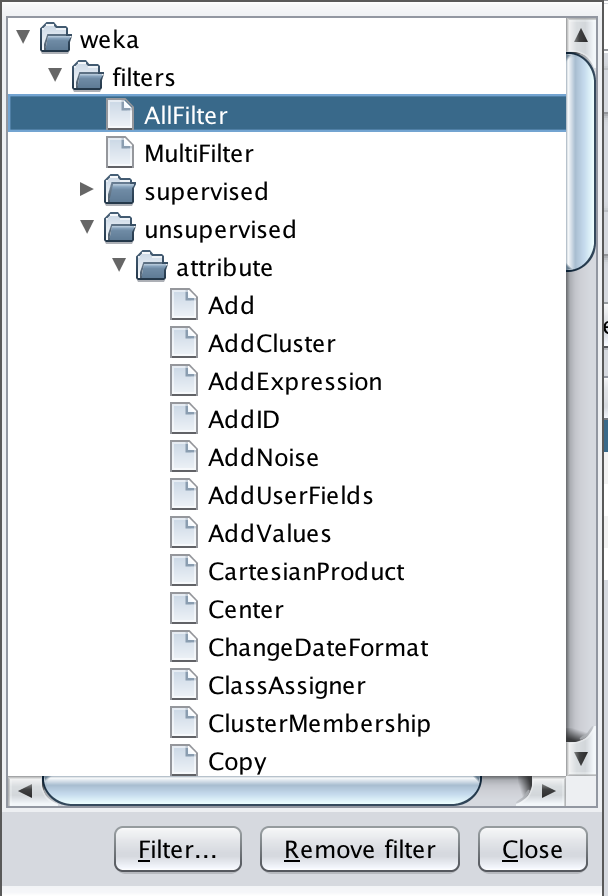
\includegraphics[width=0.45\textwidth]{images/B2_9a.png}}

\subfloat[An object editor.]{\label{subfig:filters_2}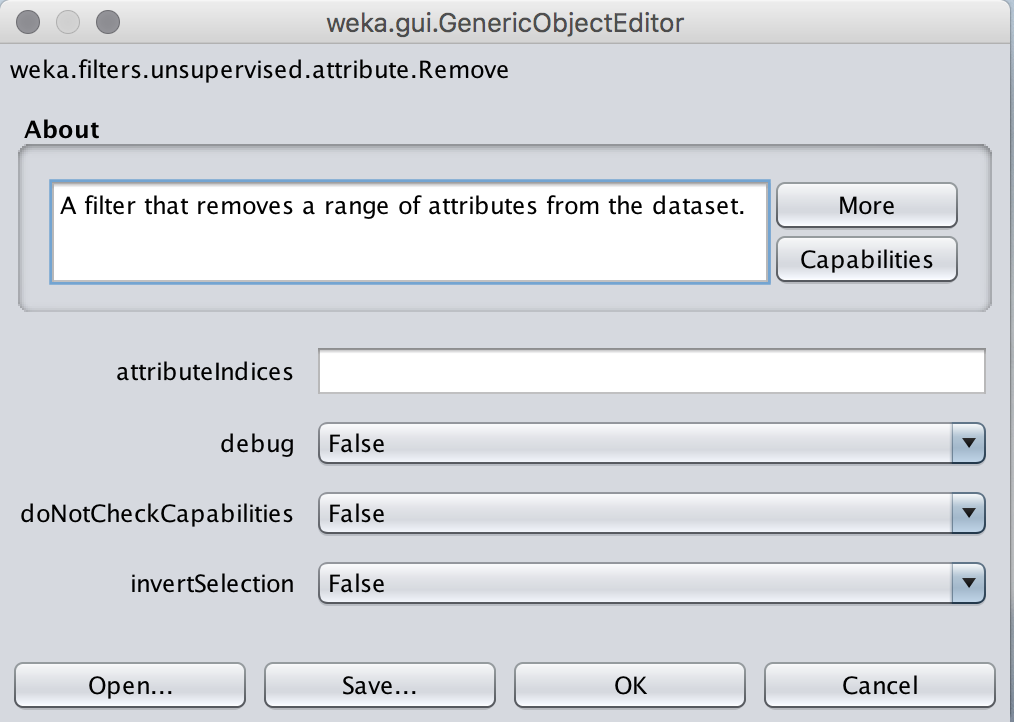
\includegraphics[width=0.45\textwidth]{images/B2_9b.png}}
\qquad
\subfloat[More information (click \textit{More}).]{\label{subfig:filters_3}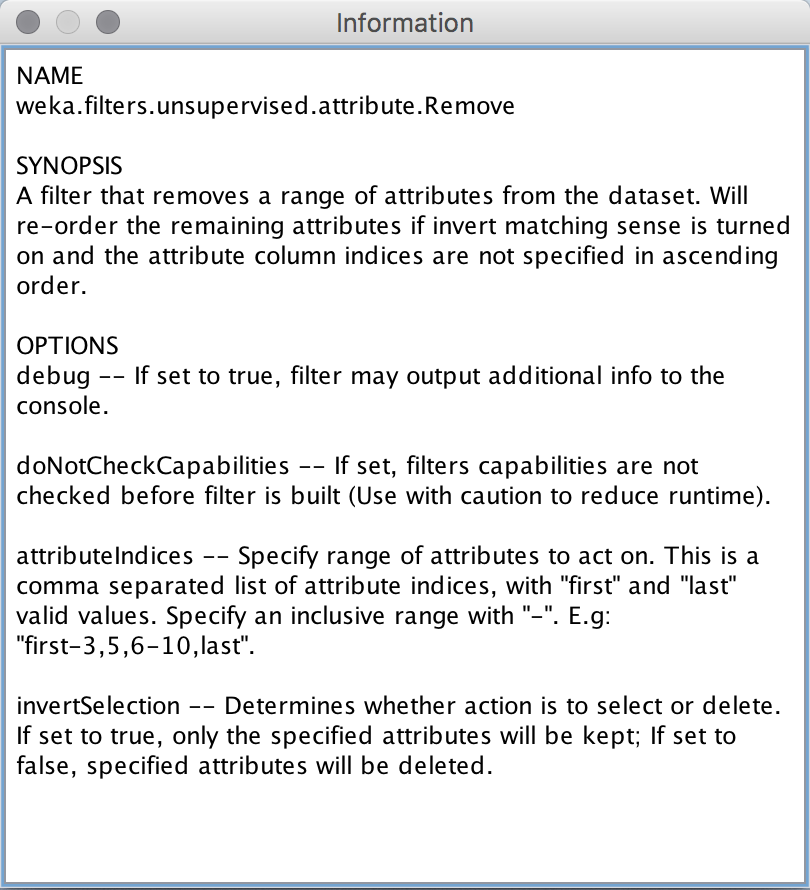
\includegraphics[width=0.45\textwidth]{images/B2_9c.png}}
\qquad
\subfloat[Information about the filter's capabilities (click \textit{Capabilities}).]{\label{subfig:filters_4}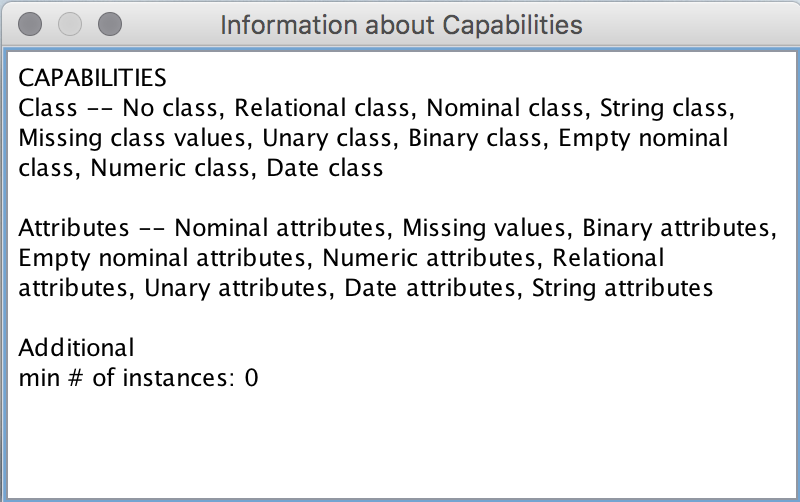
\includegraphics[width=0.45\textwidth]{images/B2_9d.png}}
\qquad
\subfloat[Constraints on capabilities.]{\label{subfig:filters_5}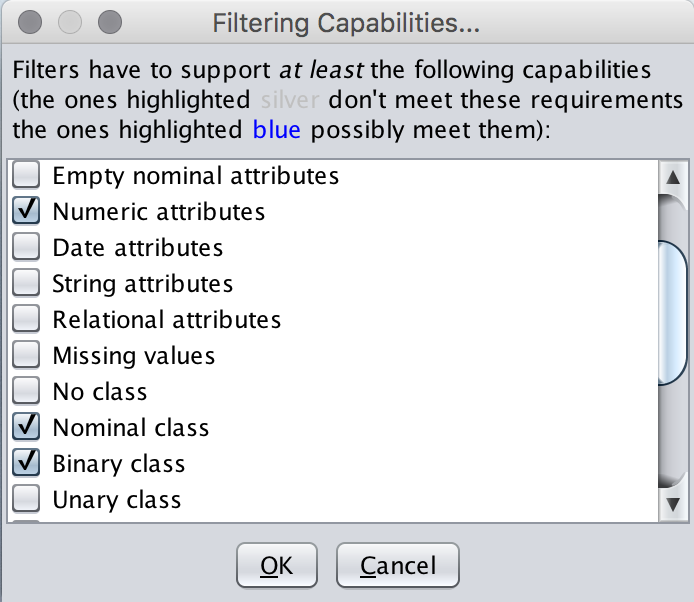
\includegraphics[width=0.45\textwidth]{images/B2_9e.png}}
\caption{\label{fig:filters}Choosing a filter.}
\end{figure}

Clicking \textit{Choose} (near the top left) in
Figure~\ref{subfig:explorer_2} gives a list of filters like that in
Figure~\ref{subfig:filters_1}. Actually, you get a collapsed version:
click on an arrow to open up its contents. We will describe how to use
a simple filter to delete specified attributes from a dataset, in
other words, to perform manual attribute selection. The same effect
can be achieved more easily by selecting the relevant attributes using
the tick boxes and pressing the \textit{Remove} button. Nevertheless
we describe the equivalent filtering operation explicitly, as an
example.

\textit{Remove} is an unsupervised attribute filter, and to see it you
must scroll further down the list. When selected, it appears in the
line beside the \textit{Choose} button, along with its parameter
values---in this case the line reads simply ``Remove''. Click that line
to bring up a generic object editor with which you can examine and
alter the filter's properties. (You did the same thing earlier by
clicking the \textit{J48} line in Figure~\ref{subfig:j48_2} to open
the \textit{J4.8} classifier's object editor.) The object editor for
the Remove filter shown in Figure~\ref{subfig:filters_2}.

To learn about it, click \textit{More} to show the information in
Figure~\ref{subfig:filters_3}. This explains that the filter removes a
range of attributes from the dataset. It has an option,
\textit{attributeIndices}, that specifies the range to act on and
another called \textit{invertSelection} that determines whether the
filter selects attributes or deletes them. There are boxes for both of
these in the object editor shown in Figure~\ref{subfig:filters_2}, and
in fact we have already set them to \textit{1,2} (to affect attributes
1 and 2, namely \textit{outlook} and \textit{temperature}) and
\textit{False} (to remove rather than retain them). Click \textit{OK}
to set these properties and close the box. Notice that the line beside
the \textit{Choose} button now reads \textit{Remove --R 1,2}. In the
command-line version of the \textit{Remove} filter, the option
\textit{--R} is used to specify which attributes to remove. After
configuring an object it's often worth glancing at the resulting
command-line formulation that the Explorer sets up.

Figure~\ref{fig:filters} demonstrates a further feature of the generic
object editor, namely ``capabilities.'' Algorithms in WEKA may provide
information about what data characteristics they can handle, and, if
they do, a \textit{Capabilities} button appears underneath
\textit{More} in the generic object editor
(Figure~\ref{subfig:filters_2}). Clicking it brings up
Figure~\ref{subfig:filters_4}, which gives information about what the
method can do. Here it states that \textit{Remove} can handle many
attribute characteristics, such as different types (nominal, numeric,
relational, etc.) and missing values. It shows the minimum number of
instances that are required for \textit{Remove} to operate on.

Figure~\ref{subfig:filters_5} shows a list of selected constraints on
capabilities, which is obtained by clicking the \textit{Filter} button
at the bottom of Figure~\ref{subfig:filters_1}. If the current dataset
exhibits some characteristic that is ticked in
Figure~\ref{subfig:filters_5} but missing from the capabilities for
the \textit{Remove} filter (Figure~\ref{subfig:filters_4}), the
\textit{Apply} button to the right of \textit{Choose} in
Figure~\ref{subfig:explorer_2} will be grayed out, as will the entry
in the list in Figure~\ref{subfig:filters_1}. Although you cannot
apply it, you can nevertheless select a grayed-out entry to inspect
its options, documentation and capabilities using the generic object
editor. You can release individual constraints by deselecting them in
Figure~\ref{subfig:filters_5}, or click the \textit{Remove filter}
button to clear all the constraints.

\begin{figure}[!ht]
\centering
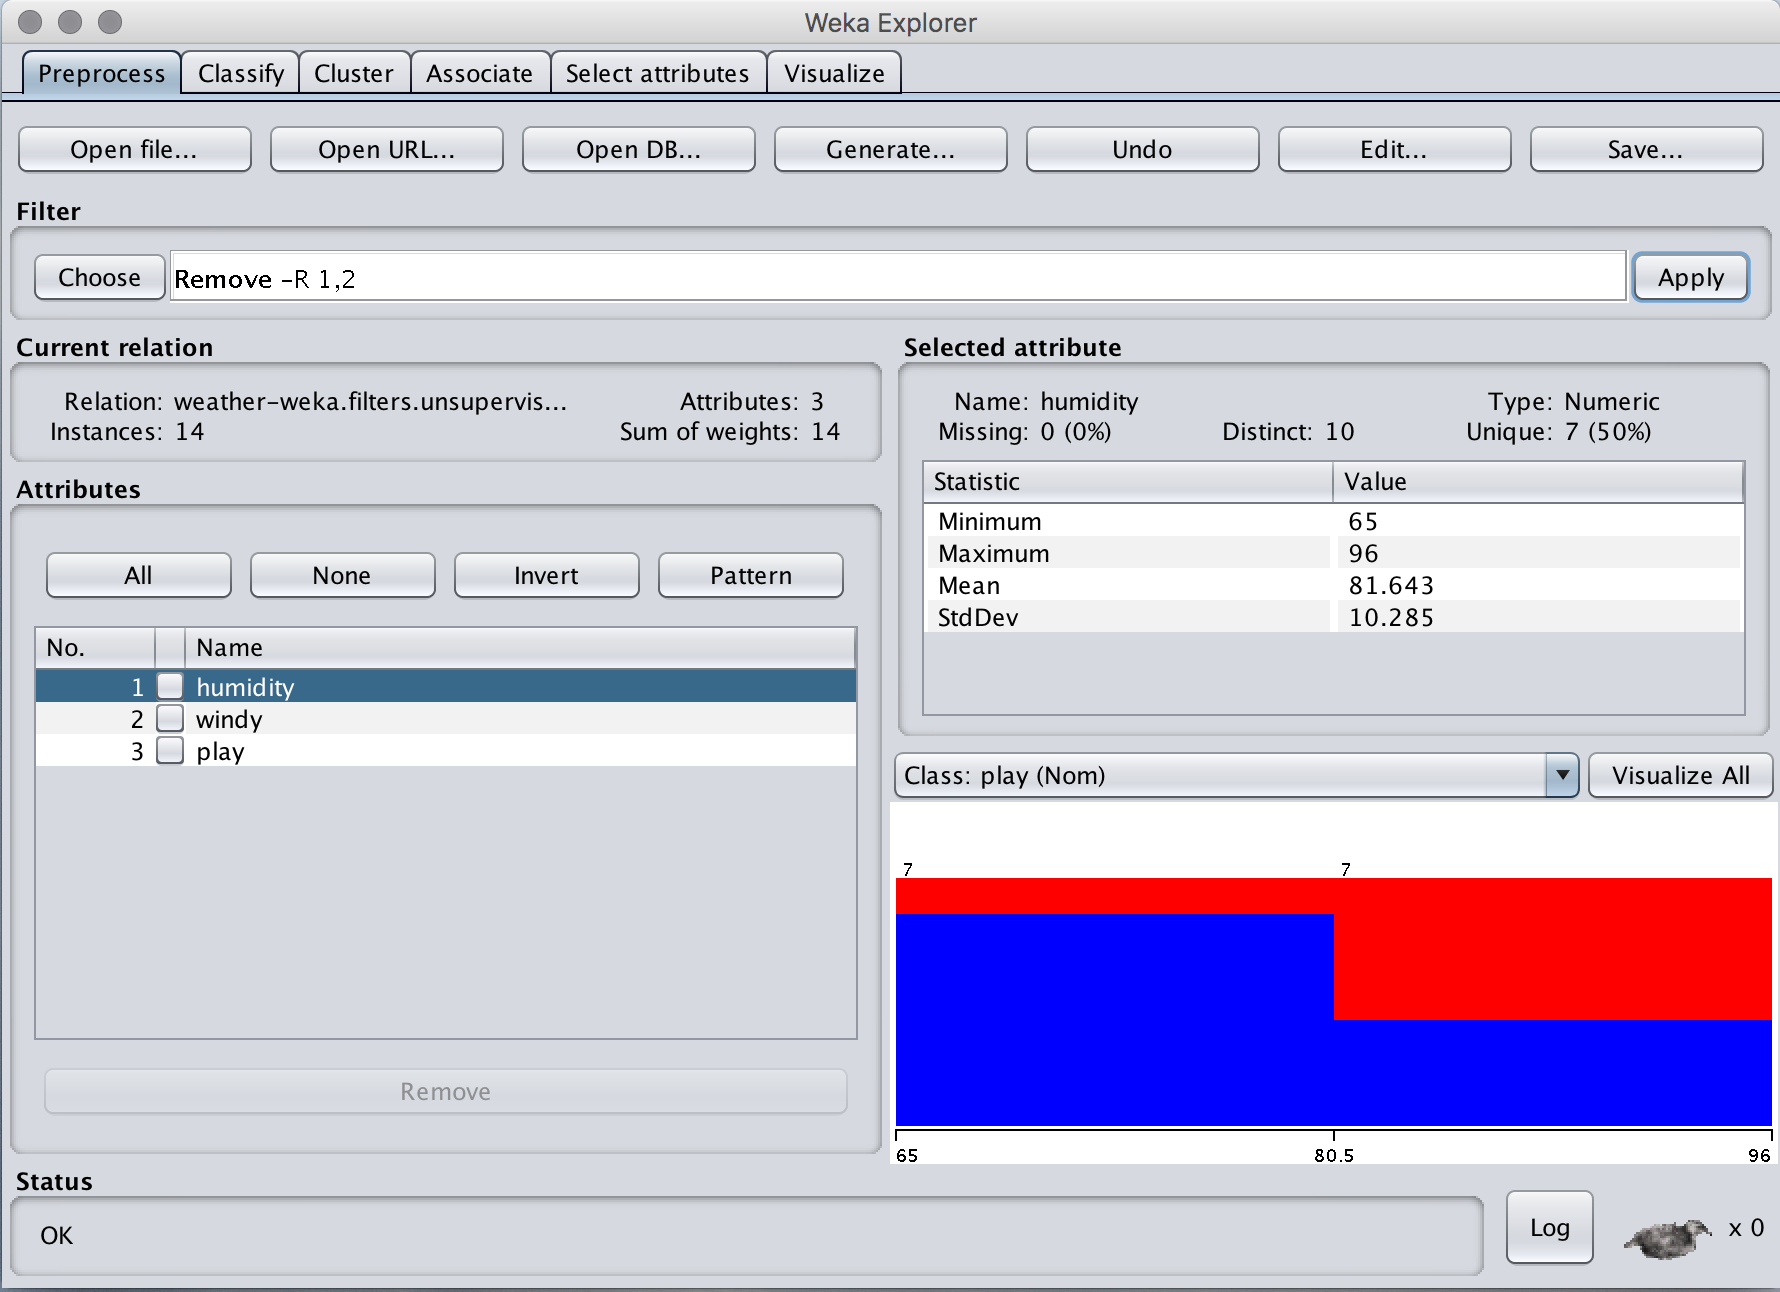
\includegraphics[width=0.9\textwidth]{images/B2_10.png}
\caption{The weather data with two attributes removed.}
\label{fig:weather_minus_two}
\end{figure}


Apply the filter by clicking \textit{Apply} (at the right-hand side of
Figure~\ref{subfig:explorer_2}). Immediately the screen in
Figure~\ref{fig:weather_minus_two} appears---just like the one in
Figure~\ref{subfig:explorer_2} but with only three attributes,
\textit{humidity}, \textit{windy}, and \textit{play}. At this point
the fifth button in the row near the top becomes active. \textit{Undo}
reverses the filtering operation and restores the original dataset,
which is useful when you experiment with different filters.

The first attribute, \textit{humidity}, is selected and a summary of
its values appears on the right. As a numeric attribute, the minimum
and maximum values, mean, and standard deviation are shown. Below is a
histogram that shows the distribution of the \textit{play}
attribute. Unfortunately, this display is impoverished because the
attribute has so few different values that they fall into two
equal-sized bins. More realistic datasets yield more informative
histograms.

\subsection{Training and testing learning schemes}

The \textit{Classify} panel lets you train and test learning schemes
that perform classification or
regression. Section~\ref{sect:getting_started} explained how to
interpret the output of a decision tree learner and showed the
performance figures that are automatically generated by the evaluation
module. The interpretation of these is the same for all models that
predict a categorical class. However, when evaluating models for
numeric prediction, WEKA produces a different set of performance
measures

\begin{figure}[!ht]
\centering
\subfloat[CPU data in the \textit{Preprocess} panel.]{\label{subfig:cpu_1}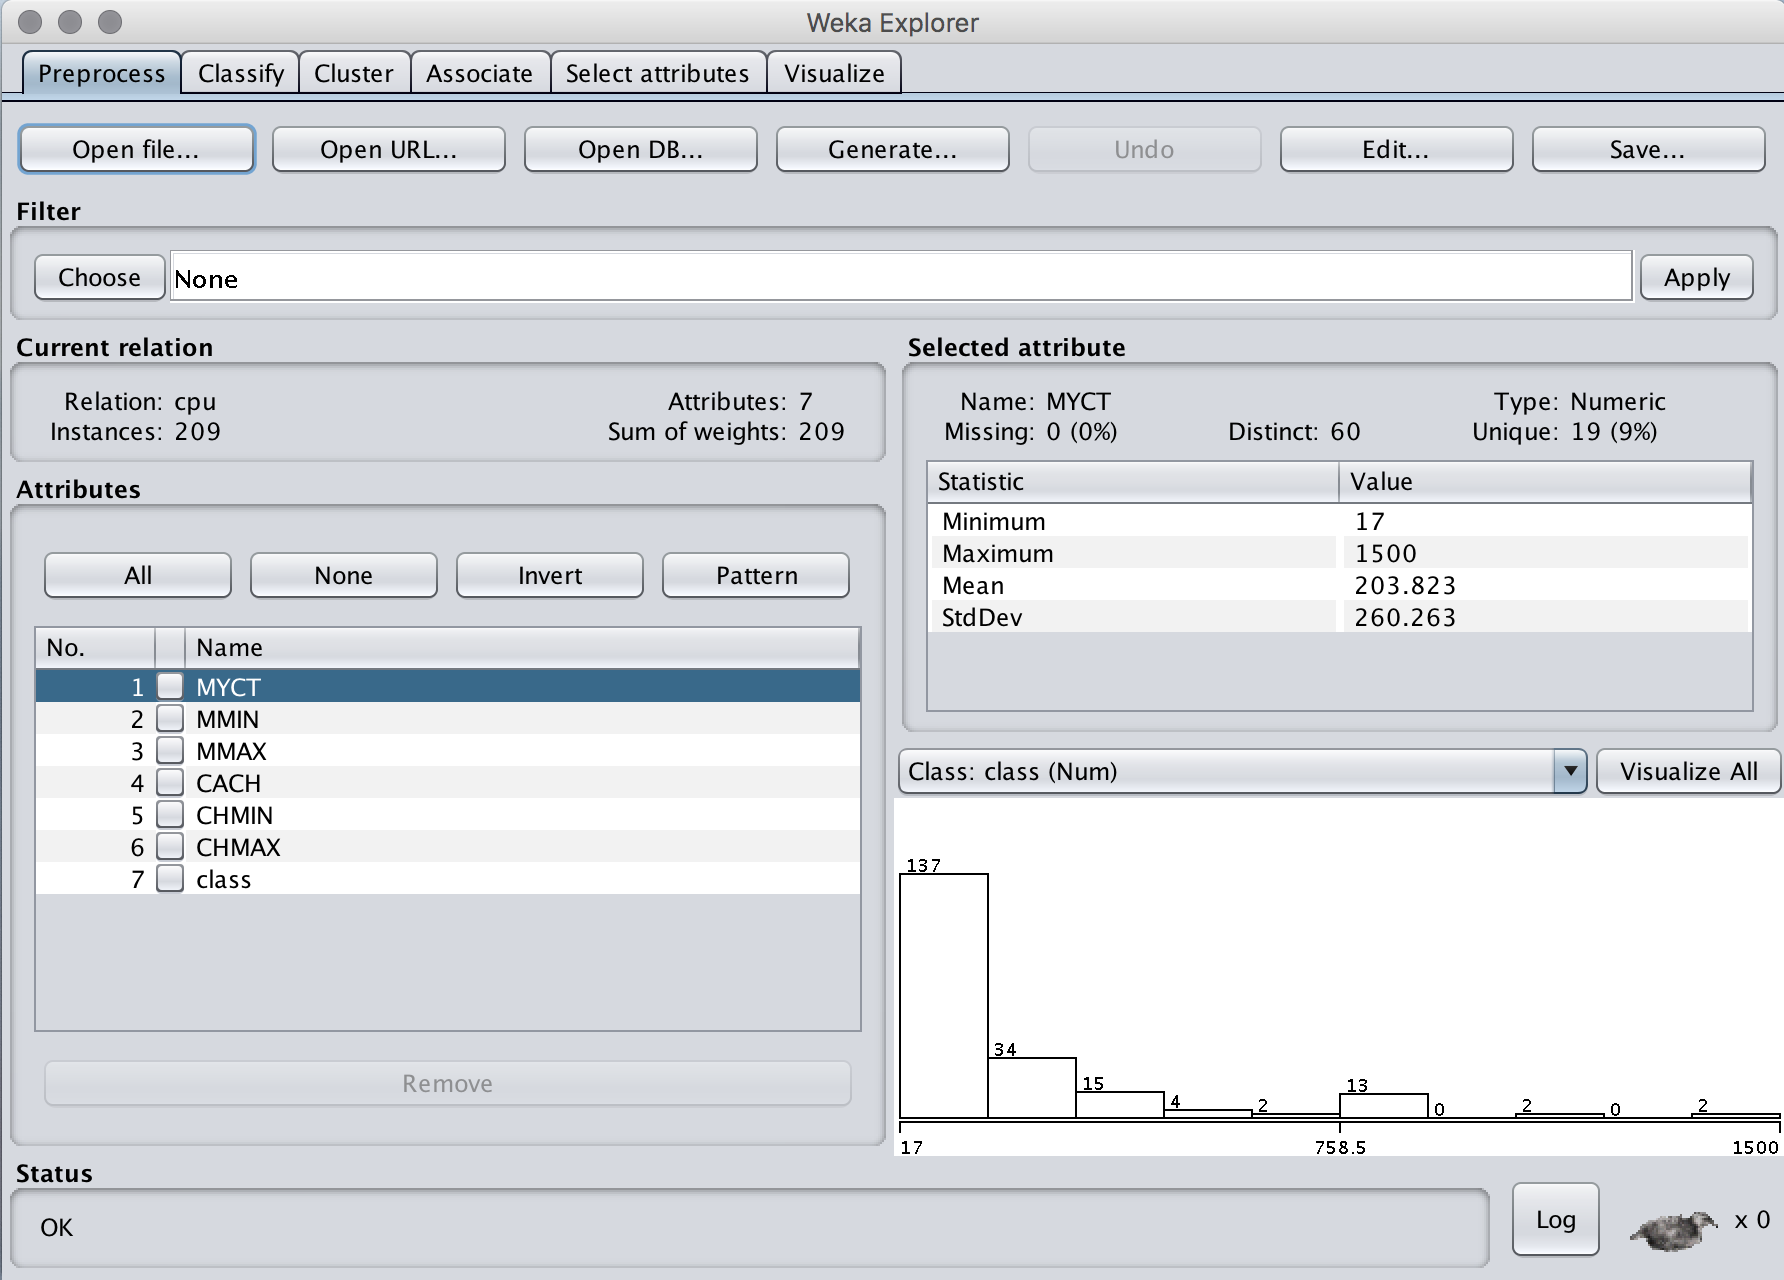
\includegraphics[width=0.9\textwidth]{images/B2_11a.png}}
\newline
\subfloat[\textit{M5'}'s performance on the CPU data.]{\label{subfig:cpu_2}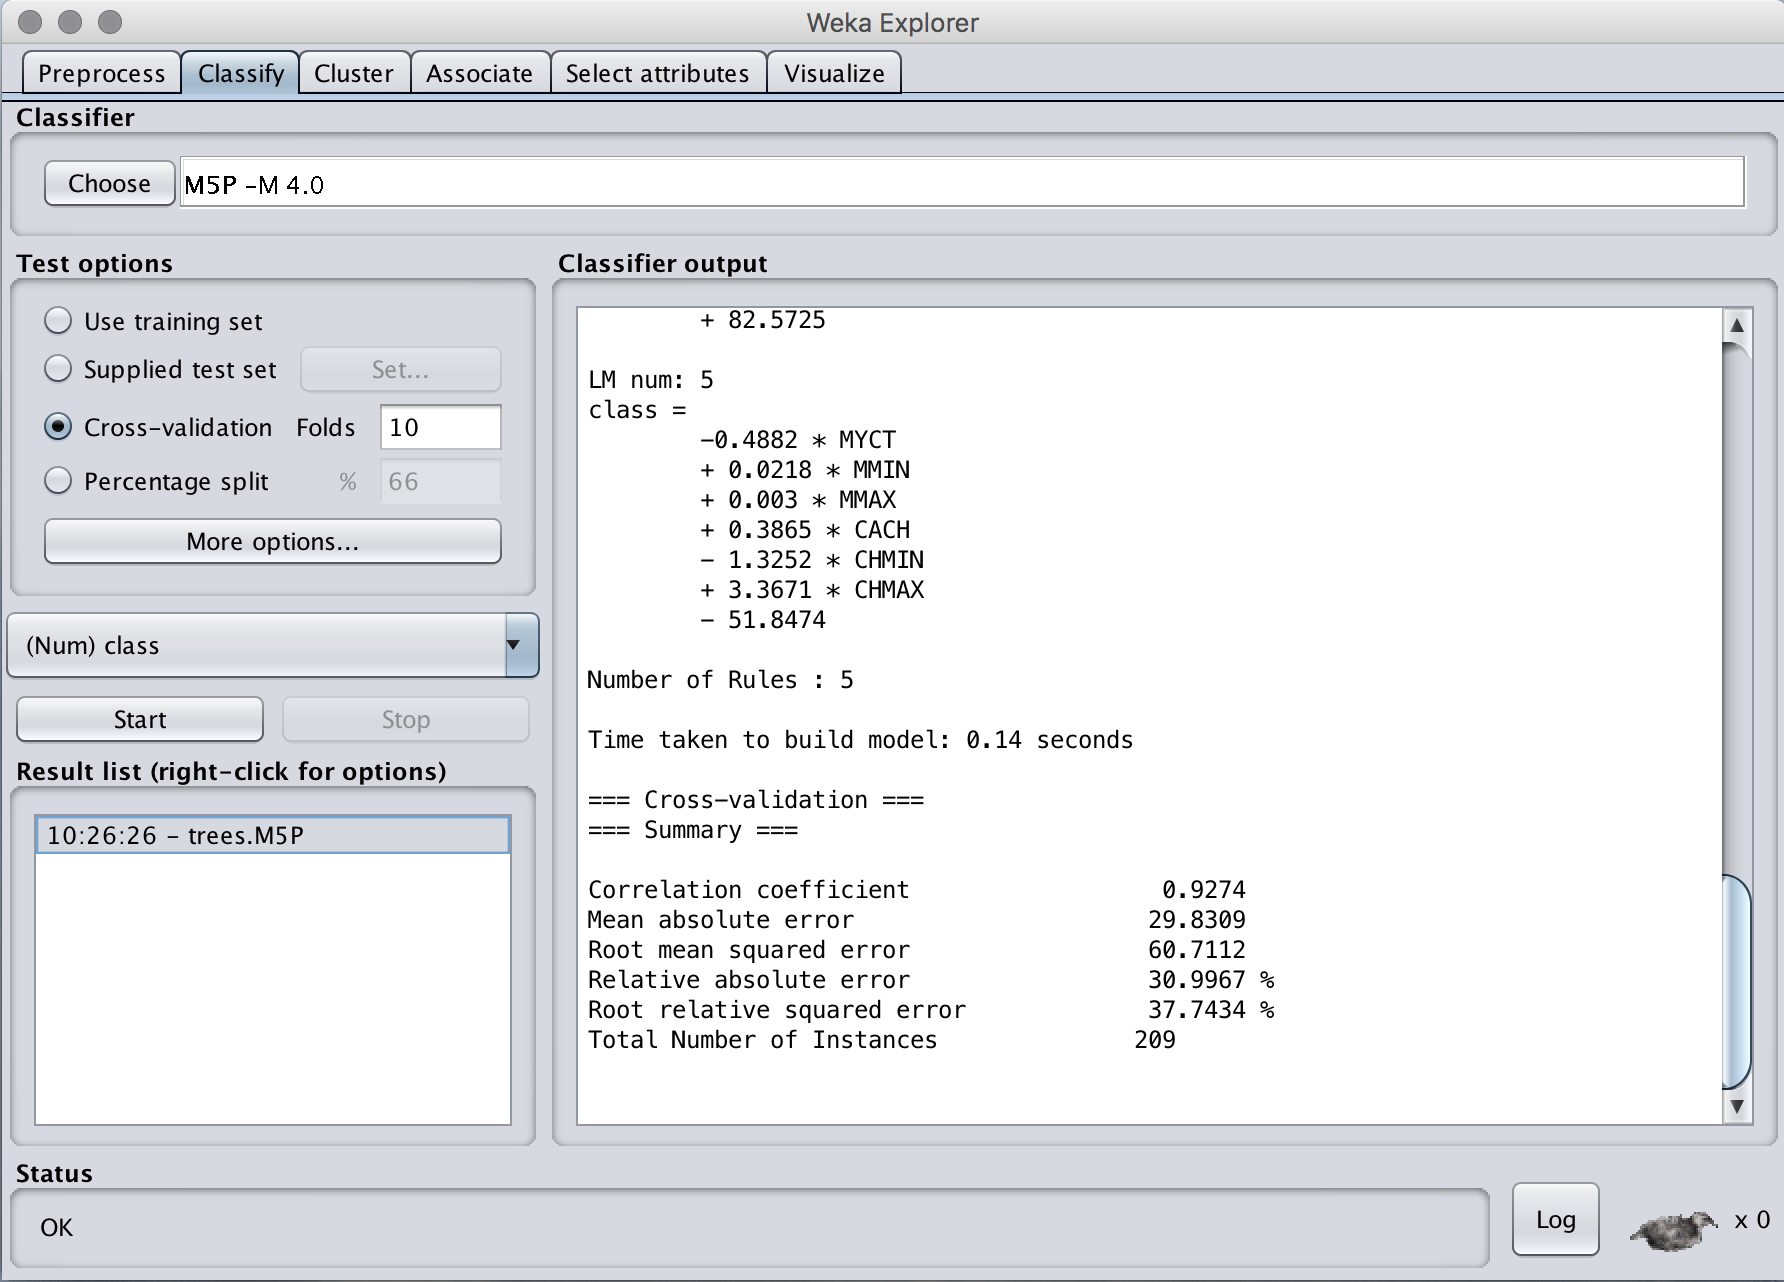
\includegraphics[width=0.9\textwidth]{images/B2_11b.png}}
\caption{\label{fig:cpu_m5}Processing the CPU performance data with \textit{M5'}.}
\end{figure}

As an example, in Figure~\ref{subfig:cpu_1} the CPU performance
dataset has been loaded into WEKA. You can see the histogram of values
of the first attribute, \textit{MYCT}, at the lower right. In
Figure~\ref{subfig:cpu_2} the model tree inducer M5' has been chosen
as the classifier by going to the \textit{Classify} panel, clicking
the \textit{Choose} button at the top left, opening up the trees
section of the hierarchical menu shown in Figure 2.4a, finding
\textit{M5P}, and clicking \textit{Start}. The hierarchy helps to
locate particular classifiers by grouping items with common
functionality

\begin{figure}[!p]
%\centering
\begin{mdframed}[innermargin=-1cm]
\begin{Verbatim}[fontsize=\footnotesize]
=== Run information ===

Scheme:       weka.classifiers.trees.M5P -M 4.0
Relation:     cpu
Instances:    209
Attributes:   7
              MYCT
              MMIN
              MMAX
              CACH
              CHMIN
              CHMAX
              class
Test mode:    10-fold cross-validation

=== Classifier model (full training set) ===

M5 pruned model tree:
(using smoothed linear models)

CHMIN <= 7.5 : LM1 (165/12.903%)
CHMIN >  7.5 : 
|   MMAX <= 28000 : 
|   |   MMAX <= 13240 : 
|   |   |   CACH <= 81.5 : LM2 (6/18.551%)
|   |   |   CACH >  81.5 : LM3 (4/30.824%)
|   |   MMAX >  13240 : LM4 (11/24.185%)
|   MMAX >  28000 : LM5 (23/48.302%)

LM num: 1
class = 
-0.0055 * MYCT + 0.0013 * MMIN + 0.0029 * MMAX + 0.8007 * CACH + 0.4015 * CHMAX 
  + 11.0971

LM num: 2
class = 
-1.0307 * MYCT + 0.0086 * MMIN + 0.0031 * MMAX + 0.7866 * CACH - 2.4503 * CHMIN 
  + 1.1597 * CHMAX + 70.8672

LM num: 3
class = -1.1057 * MYCT + 0.0086 * MMIN + 0.0031 * MMAX + 0.7995 * CACH 
  - 2.4503 * CHMIN + 1.1597 * CHMAX + 83.0016

LM num: 4
class = -0.8813 * MYCT + 0.0086 * MMIN + 0.0031 * MMAX + 0.6547 * CACH 
  - 2.3561 * CHMIN + 1.1597 * CHMAX + 82.5725

LM num: 5
class = -0.4882 * MYCT + 0.0218 * MMIN + 0.003 * MMAX + 0.3865 * CACH 
  - 1.3252 * CHMIN + 3.3671 * CHMAX - 51.8474

Number of Rules : 5

Time taken to build model: 0.14 seconds

=== Cross-validation ===
=== Summary ===

Correlation coefficient                  0.9274
Mean absolute error                     29.8309
Root mean squared error                 60.7112
Relative absolute error                 30.9967 %
Root relative squared error             37.7434 %
Total Number of Instances              209
\end{Verbatim}
\end{mdframed}
\caption{\label{fig:m5p_output}Output from the M5' program for numeric prediction.}
\end{figure}

Figure~\ref{fig:m5p_output} shows the output. The pruned model tree
contains splits on three of the six attributes in the data. The root
splits on the \textit{CHMIN} attribute, yielding a linear model at the
leaf on the left-hand branch and the remaining structure in the
right-hand branch. There are five leaves in all, each with a
corresponding linear model. The first number in parentheses at each
leaf is the number of instances that reach it; the second is the root
mean squared error of the predictions from the leaf's linear model for
those instances, expressed as a percentage of the standard deviation
of the class attribute computed over all the training data. The
description of the tree is followed by several figures that measure
its performance. These are derived from the test option chosen in
Figure 2.11b, 10-fold cross-validation (not stratified, because
stratification does not apply when the class is numeric).

Ordinary linear regression, another scheme for numeric prediction, is
found under \textit{LinearRegression} in the {\em functions} section of the
menu in Figure~\ref{subfig:j48_1}. It builds a single linear
regression model rather than the five in Figure~\ref{fig:m5p_output};
not surprisingly, its performance is slightly worse.

\begin{figure}[!ht]
\centering
\subfloat[M5'.]{\label{subfig:regression_errors_1}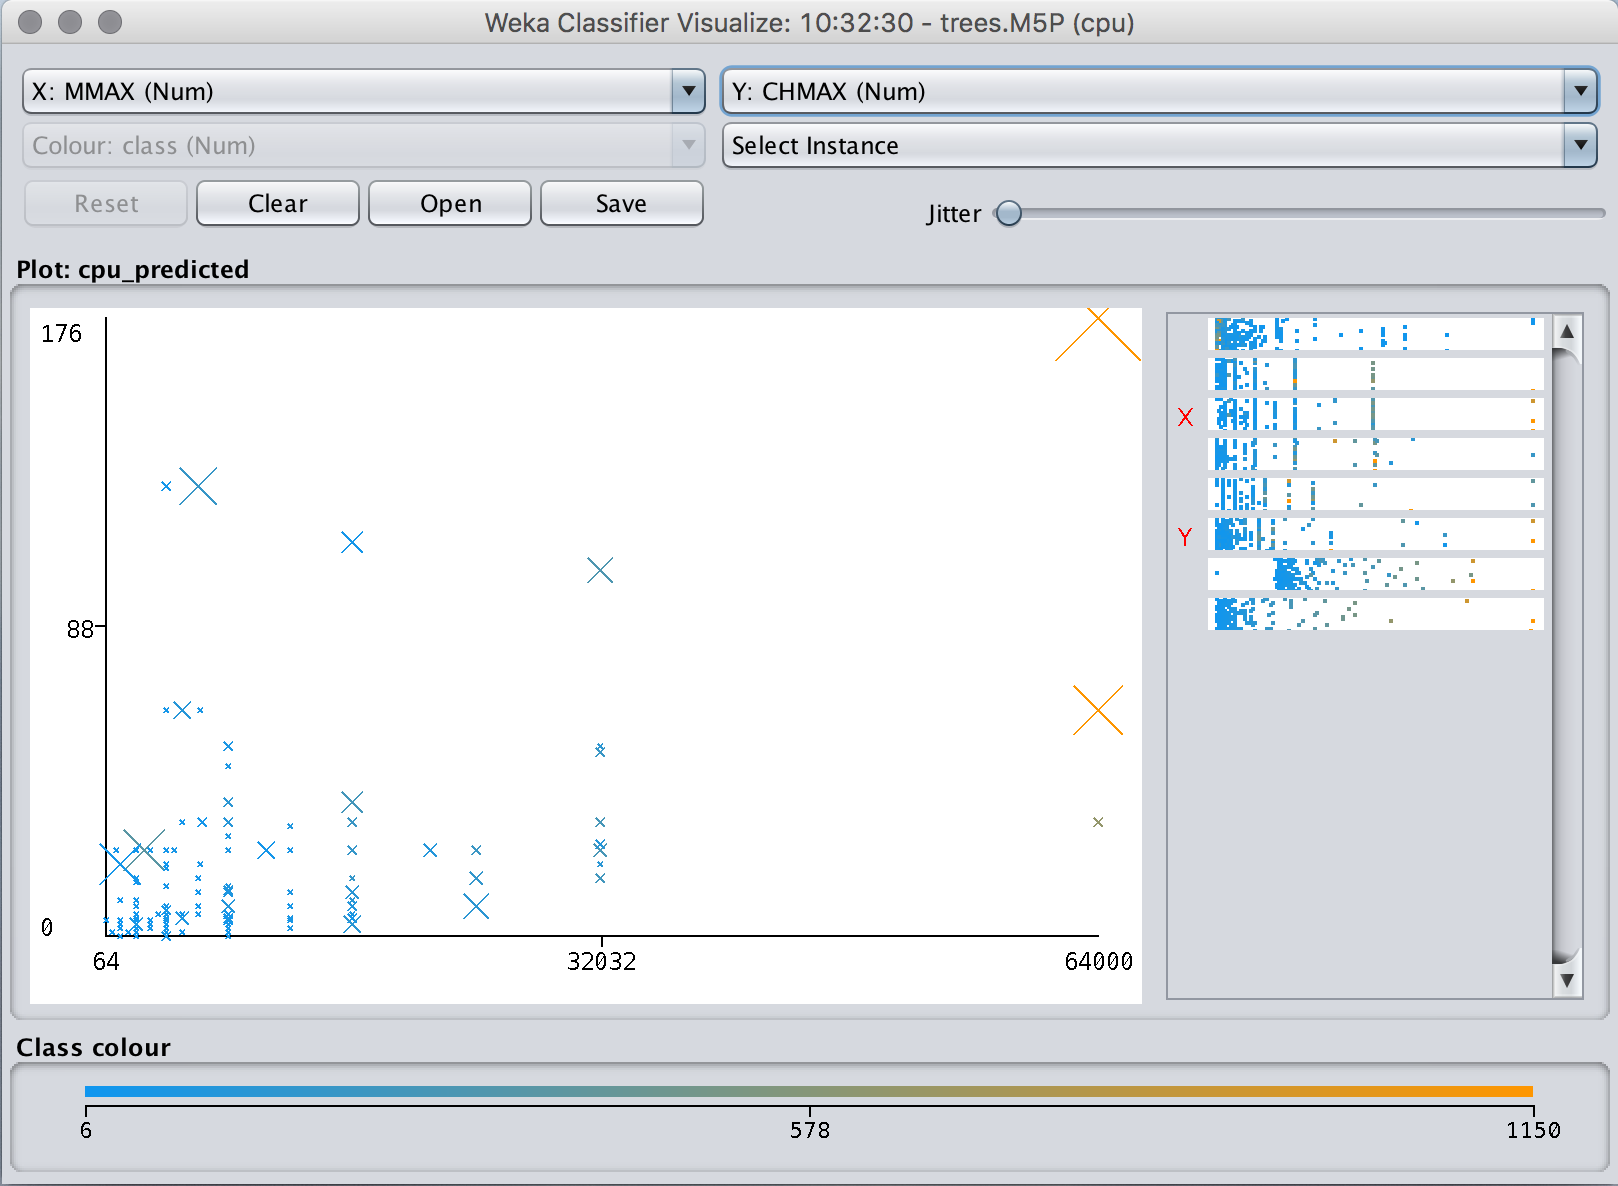
\includegraphics[width=0.9\textwidth]{images/B2_13a.png}}
\newline
\subfloat[Linear regression.]{\label{subfig:regression_errors_2}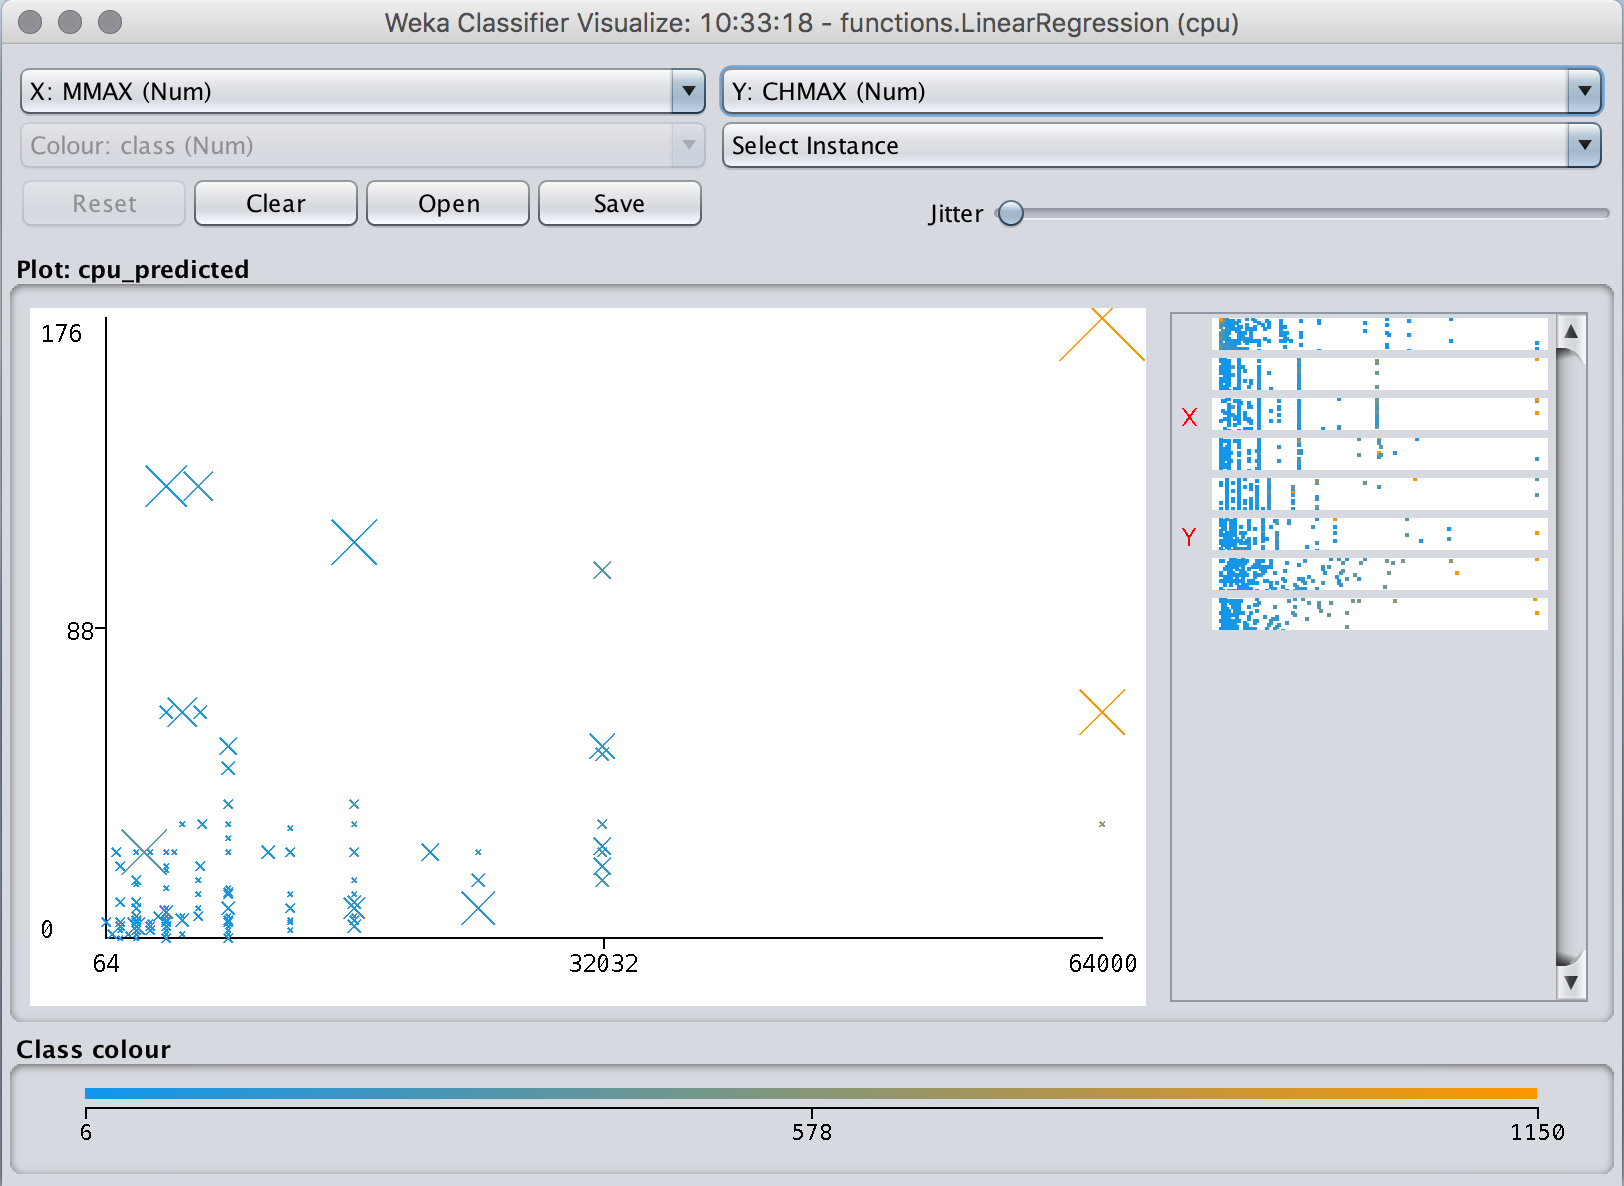
\includegraphics[width=0.9\textwidth]{images/B2_13b.png}}
\caption{\label{fig:regression_errors}Visualizing errors.}
\end{figure}


To get a feel for their relative performance, let us visualize the
errors these schemes make, as we did for the iris dataset in
Figure~\ref{subfig:j48_4}. Right-click the entry in the history list
and select \textit{Visualize classifier errors} to bring up the
two-dimensional plot of the data in
Figure~\ref{fig:regression_errors}. The points are color coded by
class---but in this case the color varies continuously because the
class is numeric. In Figure~\ref{fig:regression_errors} the
\textit{MMAX} attribute has been selected for the X-axis and
\textit{CHMAX} has been chosen for the Y-axis because this gives a
reasonable spread of points. Each data point is marked by a cross
whose size indicates the absolute value of the error for that
instance. The smaller crosses in
Figure~\ref{subfig:regression_errors_1} (for M5'), when compared with
those in Figure~\ref{subfig:regression_errors_2} (for linear
regression), show that M5' is superior.

\subsection{Using a metalearner}

\begin{figure}[!ht]
\centering
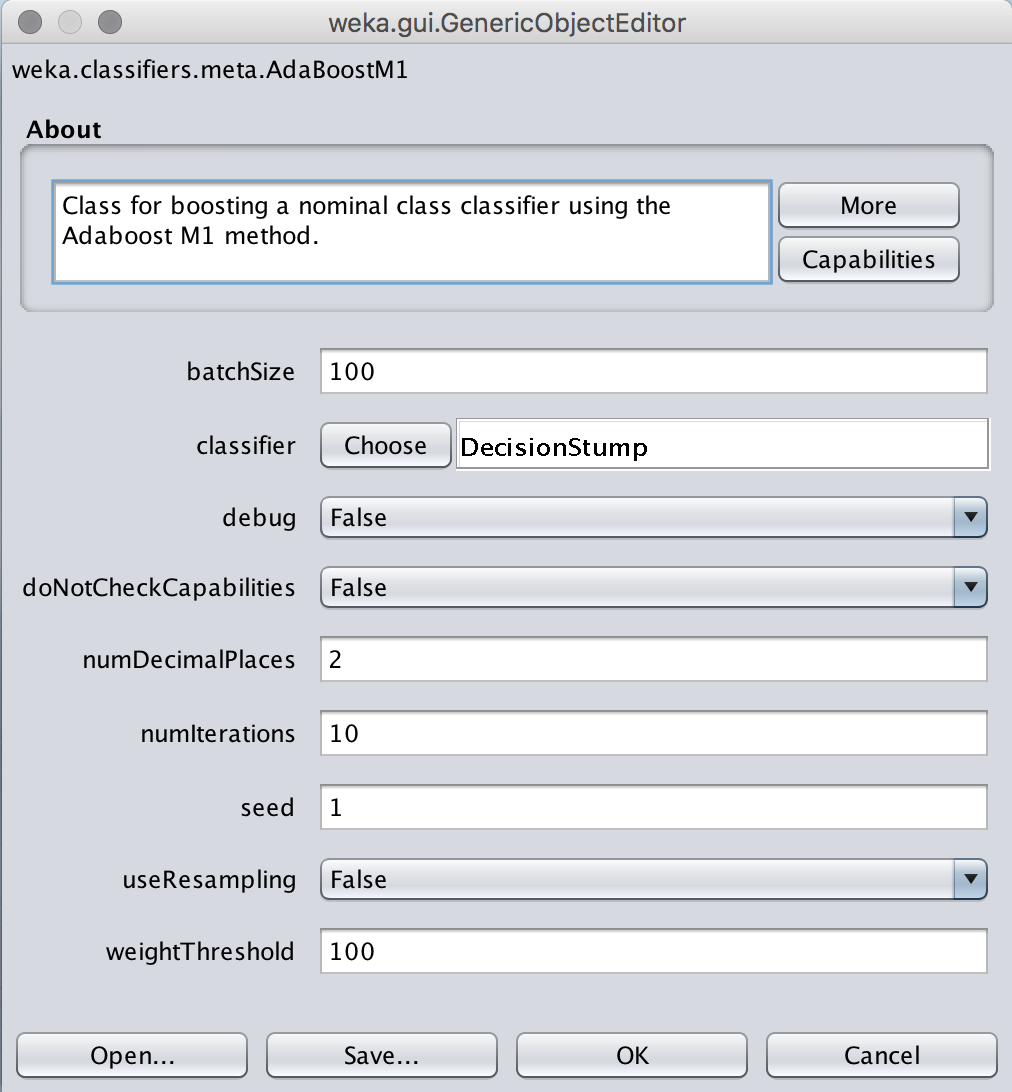
\includegraphics[width=0.7\textwidth]{images/B2_14.png}
\caption{Configuring a metalearner for boosting decision stumps.}
\label{fig:config_metalearner}
\end{figure}


Metalearners take simple classifiers and turn them into more powerful
learners. For example, to boost decision stumps in the Explorer, go to
the \textit{Classify} panel and choose the classifier
\textit{AdaboostM1} from the meta section of the hierarchical
menu. When you configure this classifier by clicking it, the object
editor shown in Figure~\ref{fig:config_metalearner} appears. This has
its own classifier field, which we set to \textit{DecisionStump} (as
shown). This method could itself be configured by clicking (except
that \textit{DecisionStump} happens to have no editable
properties). Click \textit{OK} to return to the main \textit{Classify}
panel and {\em Start} to try out boosting decision stumps up to 10 times. It
turns out that this mislabels only 7 of the 150 instances in the iris
data---good performance considering the rudimentary nature of decision
stumps and the rather small number of boosting iterations.

\subsection{Clustering and association rules}

Use the \textit{Cluster} and \textit{Associate} panels to invoke
clustering algorithms and methods for finding association rules. When
clustering, WEKA shows the number of clusters and how many instances
each cluster contains. For some algorithms the number of clusters can
be specified by setting a parameter in the object editor. For
probabilistic clustering methods, WEKA measures the log-likelihood of
the clusters on the training data: the larger this quantity, the
better the model fits the data. Increasing the number of clusters
normally increases the likelihood, but may overfit.

The controls on the \textit{Cluster} panel are similar to those for
\textit{Classify}. You can specify some of the same evaluation
methods---use training set, supplied test set, and percentage split
(the last two are used with the log-likelihood). A further method,
classes to clusters evaluation, compares how well the chosen clusters
match a preassigned class in the data. You select an attribute (which
must be nominal) that represents the ``true'' class. Having clustered
the data, WEKA determines the majority class in each cluster and
prints a confusion matrix showing how many errors there would be if
the clusters were used instead of the true class. If your dataset has
a class attribute, you can ignore it during clustering by selecting it
from a pull-down list of attributes, and see how well the clusters
correspond to actual class values. Finally, you can choose whether or
not to store the clusters for visualization. The only reason not to do
so is to conserve space. As with classifiers, you visualize the
results by right-clicking on the result list, which allows you to view
two-dimensional scatter plots like the one in
Figure~\ref{subfig:j48_4}. If you have chosen classes to clusters
evaluation, the class assignment errors are shown. For the
\textit{Cobweb} clustering scheme, you can also visualize the tree.

\begin{figure}[!ht]
%\centering
\begin{mdframed}[innermargin=-1.5cm]
\begin{Verbatim}[fontsize=\scriptsize]
 1. outlook=overcast 4 ==> play=yes 4 <conf:(1)> lift:(1.56) lev:(0.1) [1] conv:(1.43)
 2. temperature=cool 4 ==> humidity=normal 4 <conf:(1)> lift:(2) lev:(0.14) [2] conv:(2)
 3. humidity=normal windy=FALSE 4 ==> play=yes 4 <conf:(1)> lift:(1.56) lev:(0.1) [1] conv:(1.43)
 4. outlook=sunny play=no 3 ==> humidity=high 3 <conf:(1)> lift:(2) lev:(0.11) [1] conv:(1.5)
 5. outlook=sunny humidity=high 3 ==> play=no 3 <conf:(1)> lift:(2.8) lev:(0.14) [1] conv:(1.93)
 6. outlook=rainy play=yes 3 ==> windy=FALSE 3 <conf:(1)> lift:(1.75) lev:(0.09) [1] conv:(1.29)
 7. outlook=rainy windy=FALSE 3 ==> play=yes 3 <conf:(1)> lift:(1.56) lev:(0.08) [1] conv:(1.07)
 8. temperature=cool play=yes 3 ==> humidity=normal 3 <conf:(1)> lift:(2) lev:(0.11) [1] conv:(1.5)
 9. outlook=sunny temperature=hot 2 ==> humidity=high 2 <conf:(1)> lift:(2) lev:(0.07) [1] conv:(1)
10. temperature=hot play=no 2 ==> outlook=sunny 2 <conf:(1)> lift:(2.8) lev:(0.09) [1] conv:(1.29)
\end{Verbatim}
\end{mdframed}
\caption{\label{fig:apriori_output}Output from the Apriori program for association rules.}
\end{figure}

The \textit{Associate} panel is simpler than \textit{Classify} or
\textit{Cluster}. WEKA contains several algorithms for determining
association rules and no methods for evaluating such
rules. Figure~\ref{fig:apriori_output} shows the output from the
Apriori program for association rules on the nominal version of the
weather data. Despite the simplicity of the data, several rules are
found. The number before the arrow is the number of instances for
which the antecedent is true; that after the arrow is the number of
instances for which the consequent is true also; and the confidence
(in parentheses) is the ratio between the two. Ten rules are found by
default: you can ask for more by using the object editor to change
\textit{numRules}.

\subsection{Attribute selection}

The \textit{Select attributes} panel gives access to several methods
for attribute selection. This involves an attribute evaluator and a
search method. Both are chosen in the usual way and configured with
the object editor. You must also decide which attribute to use as the
class. Attribute selection can be performed using the full training
set or using cross-validation. In the latter case it is done
separately for each fold, and the output shows how many times---that is,
in how many of the folds---each attribute was selected. The results are
stored in the history list. When you right-click an entry here you can
visualize the dataset in terms of the selected attributes (choose
\textit{Visualize reduced data}).

\subsection{Visualization}

\begin{figure}[!p]
\centering
\subfloat[Scatter plot matrix.]{\label{subfig:visualize_1}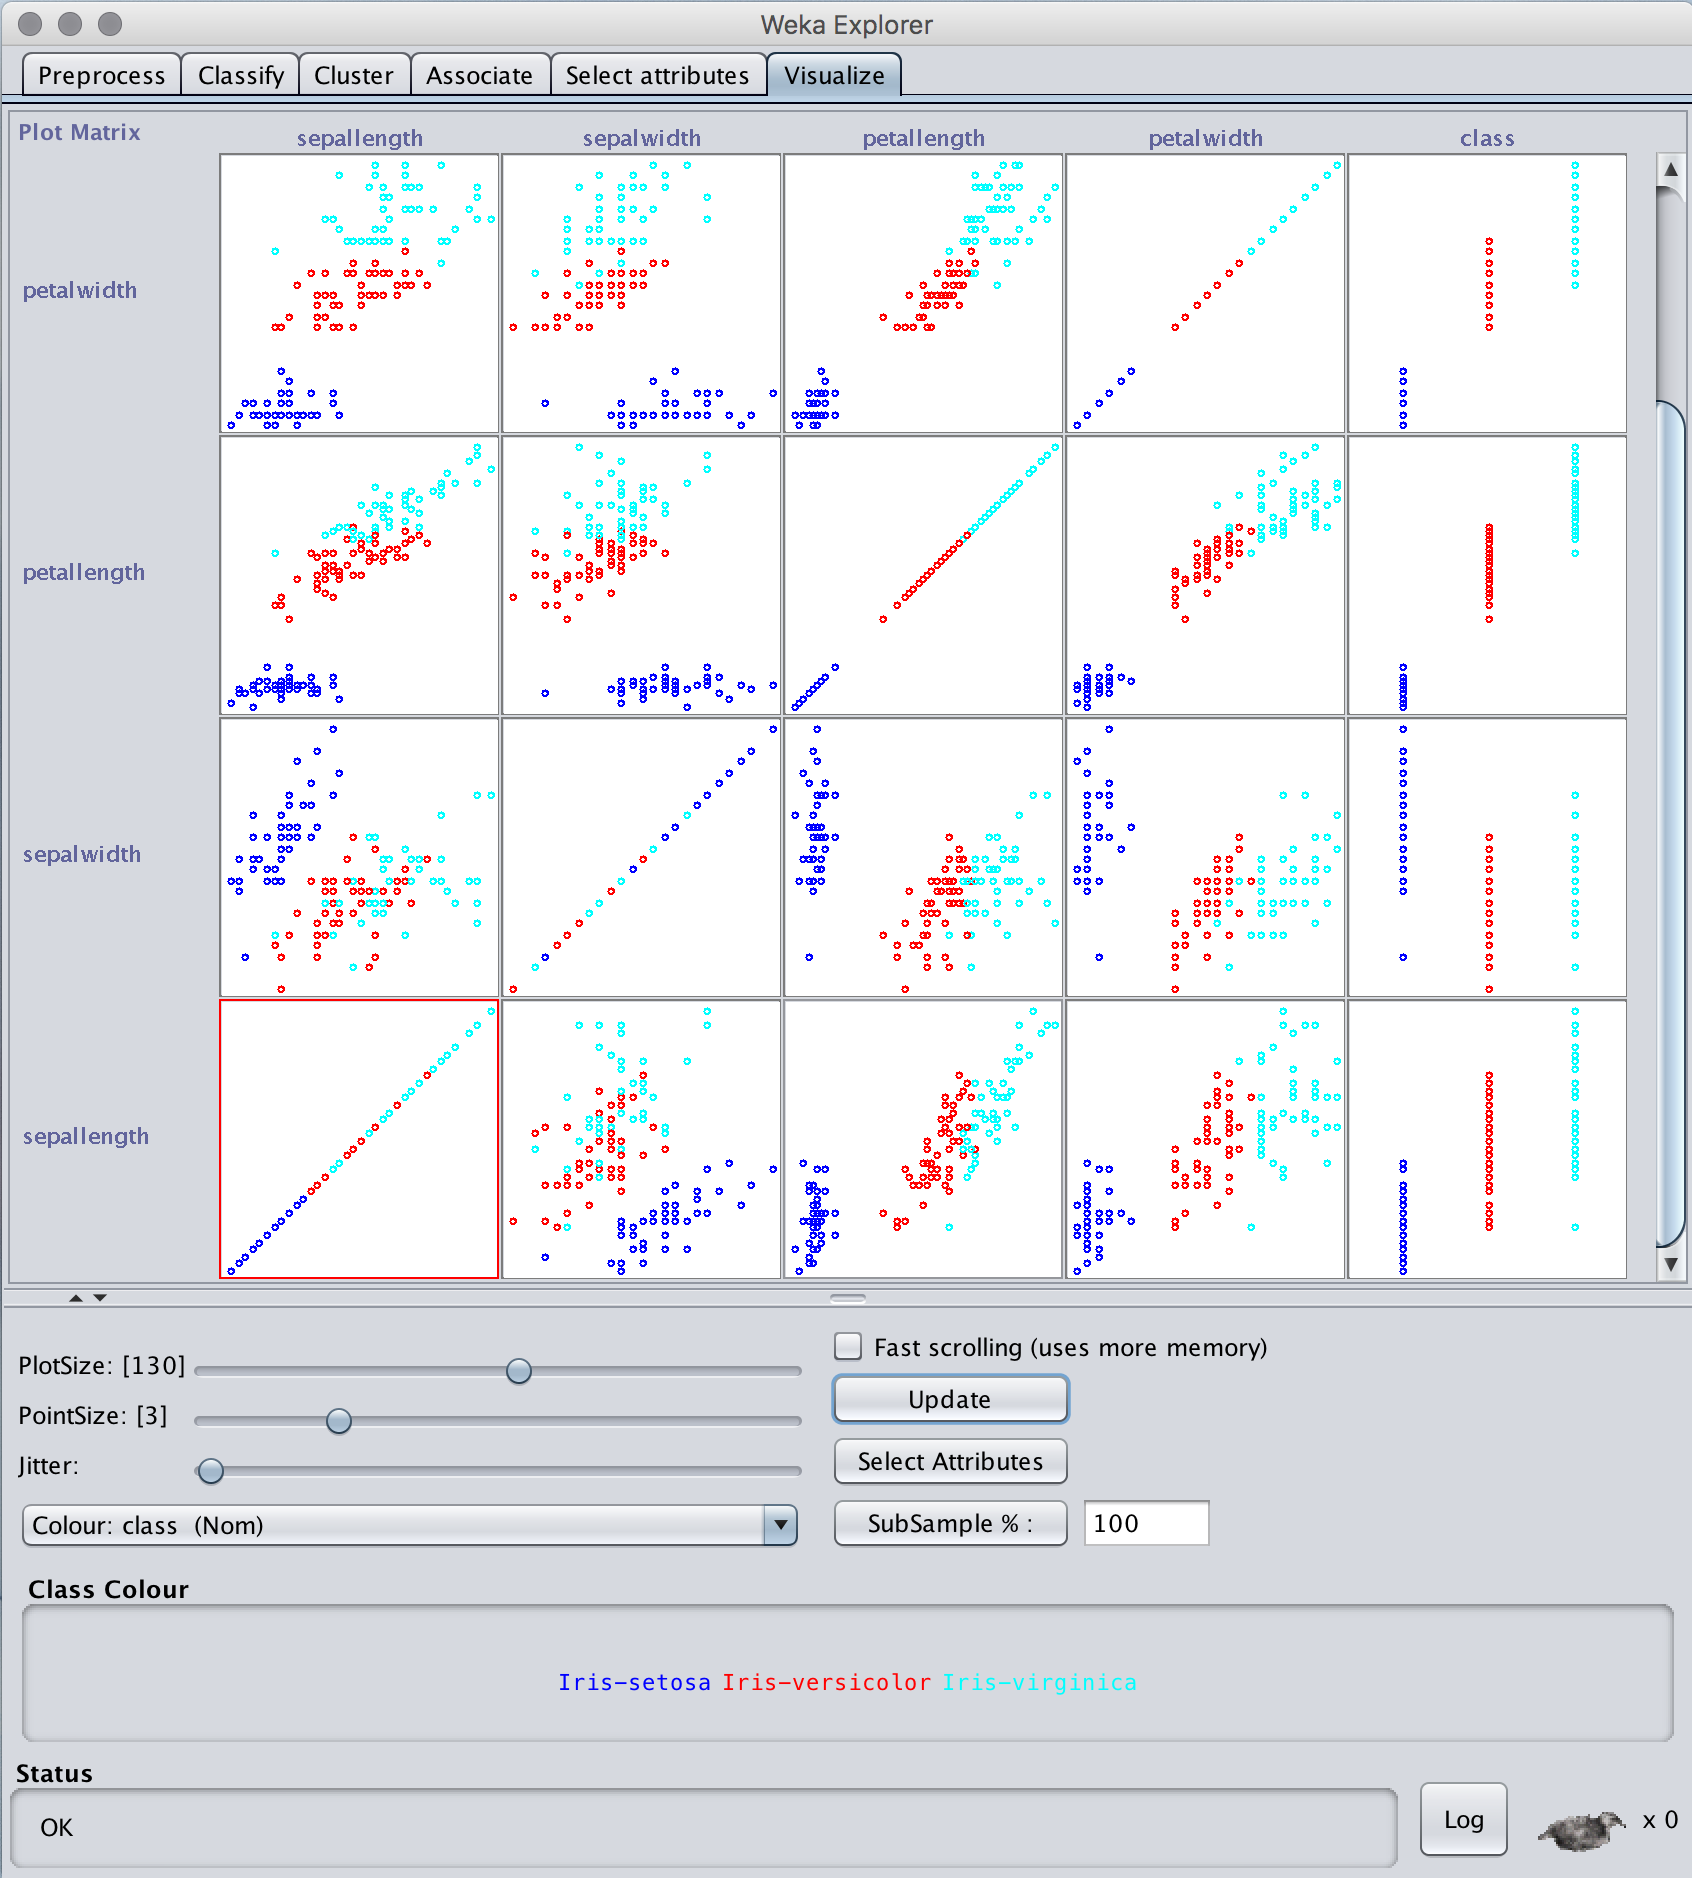
\includegraphics[width=0.8\textwidth]{images/B2_16a.png}}
\newline
\subfloat[Zoomed in on a cell from the matrix.]{\label{subfig:visualize_2}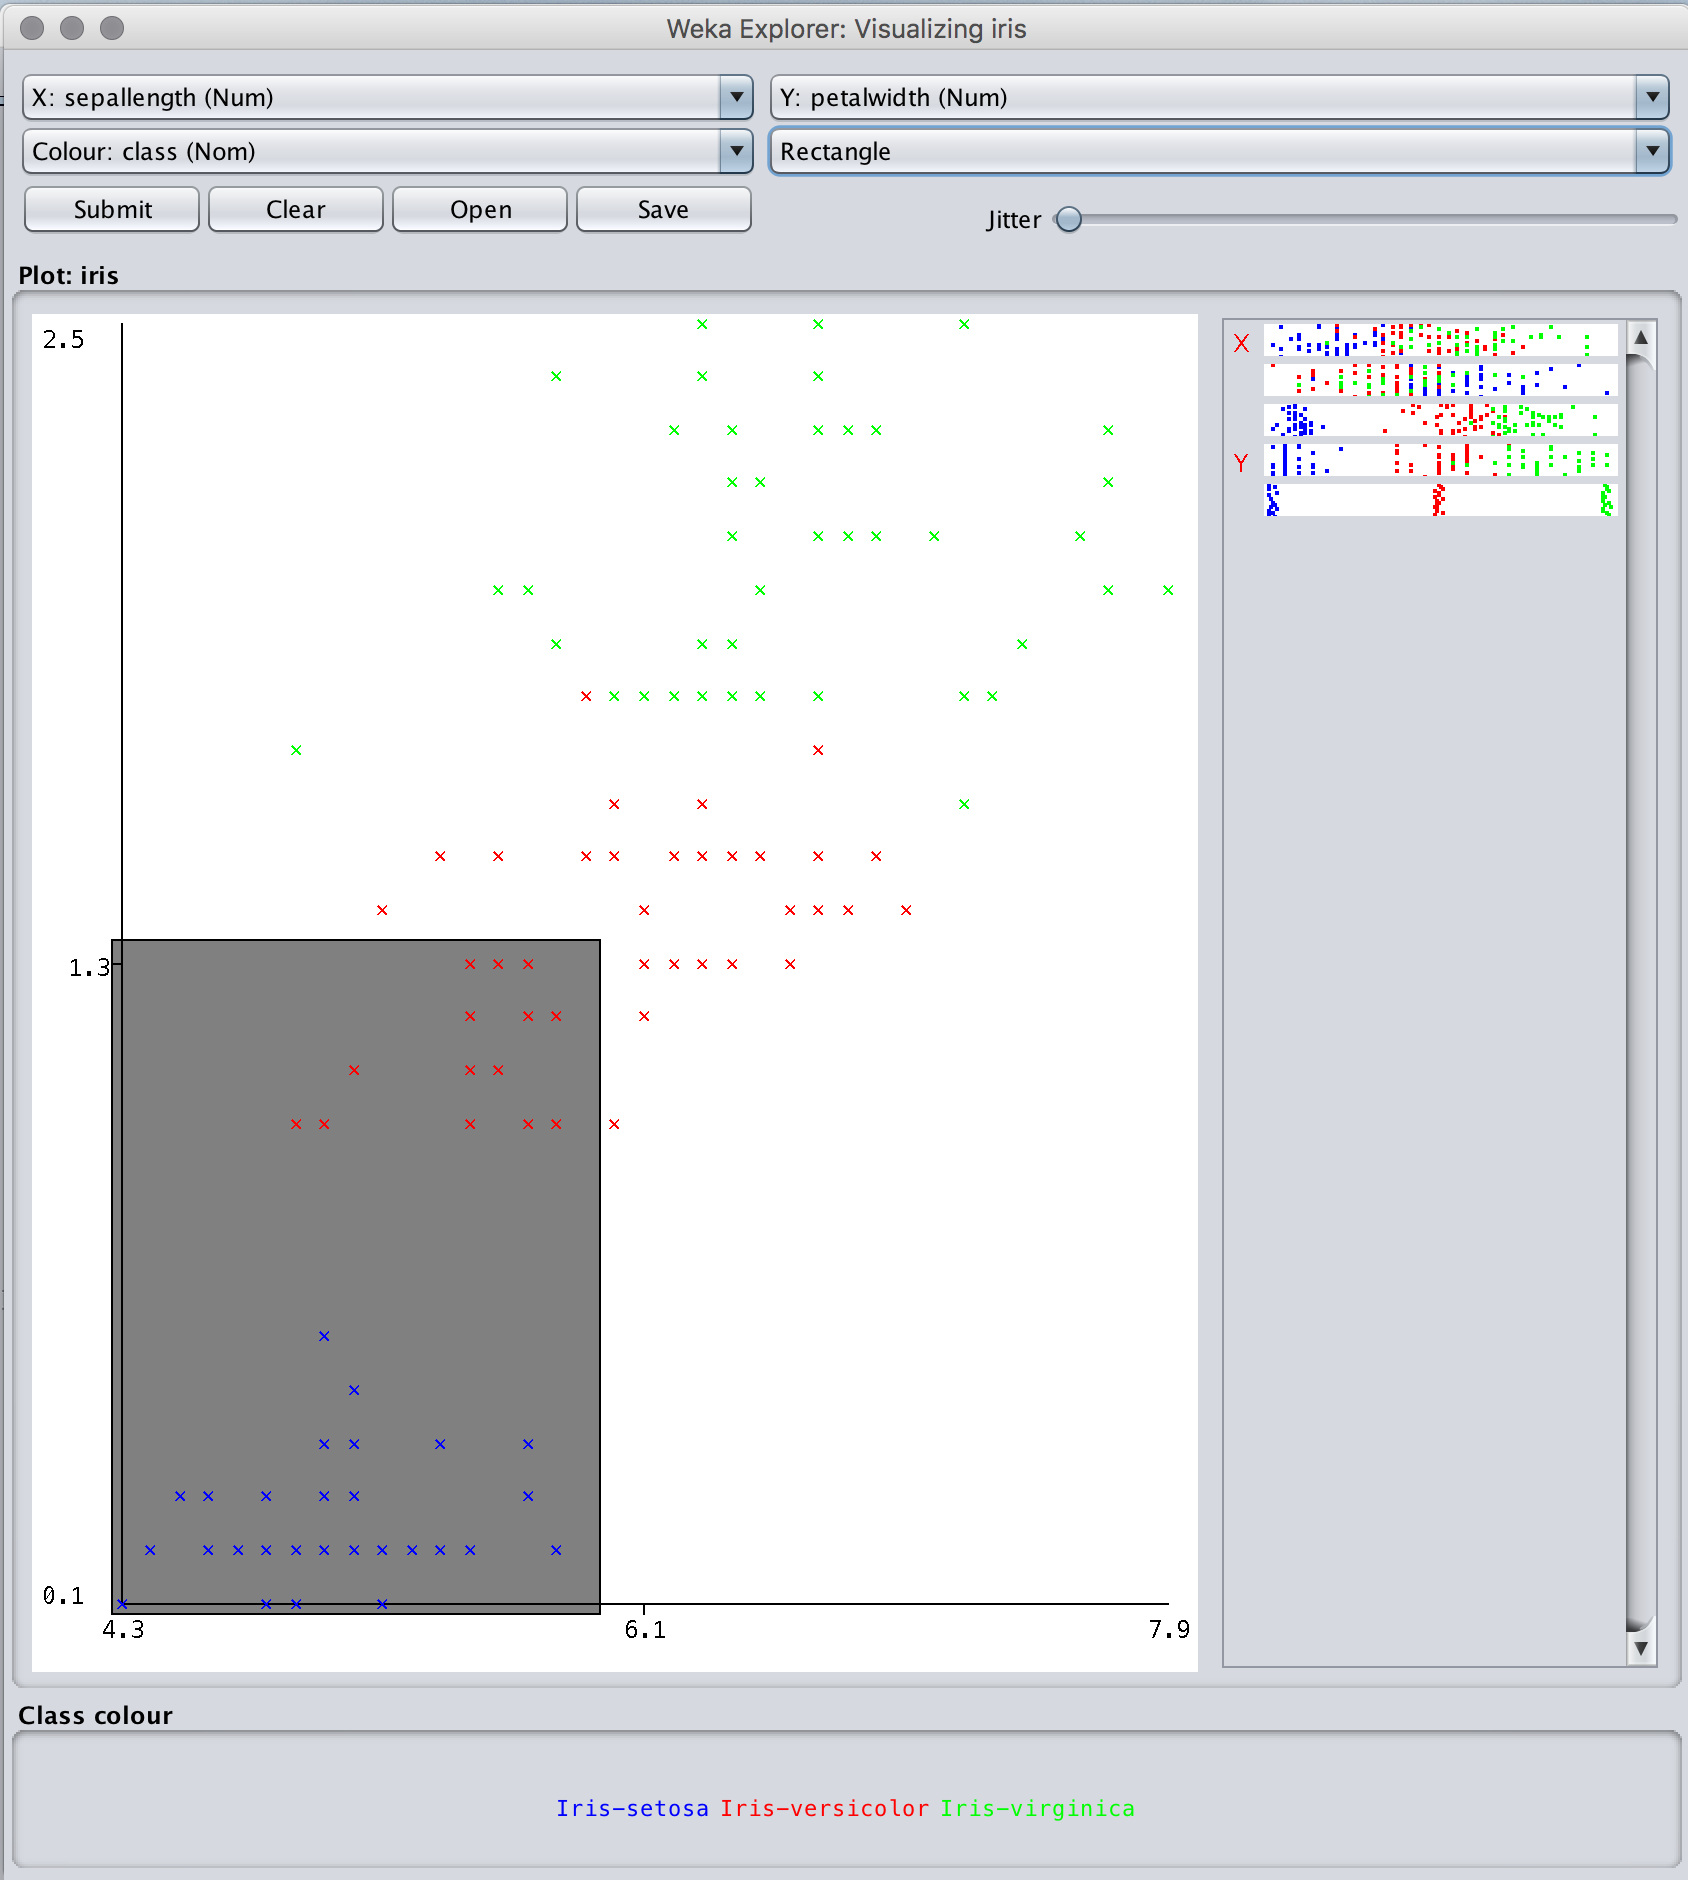
\includegraphics[width=0.8\textwidth]{images/B2_16b.png}}
\caption{\label{fig:regression_errors}Visualizing the iris data.}
\end{figure}


The \textit{Visualize} panel helps you visualize a dataset---not the
result of a classification or clustering model, but the dataset
itself. It displays a matrix of two-dimensional scatter plots of every
pair of attributes. Figure~\ref{subfig:visualize_1} shows the iris dataset. You can
select an attribute---normally the class---for coloring the data
points using the controls at the bottom. If it is nominal, the
coloring is discrete; if it is numeric, the color spectrum ranges
continuously from blue (low values) to orange (high values). Data
points with no class value are shown in black. You can change the size
of each plot, the size of the points, and the amount of jitter, which
is a random displacement applied to X and Y values to separate points
that lie on top of one another. Without jitter, a thousand instances
at the same data point would look just the same as one instance. You
can reduce the size of the matrix of plots by selecting certain
attributes, and you can subsample the data for efficiency. Changes in
the controls do not take effect until the \textit{Update} button is
clicked.

Click one of the plots in the matrix to enlarge it. For example,
clicking on the top left plot brings up the panel in
Figure~\ref{subfig:visualize_2}. You can zoom in on any area of this
panel by choosing \textit{Rectangle} from the menu near the top right
and dragging out a rectangle on the viewing area like that shown. The
\textit{Submit} button near the top left rescales the rectangle into
the viewing area.

\section{Filtering algorithms}

Now we take a detailed look at the filtering algorithms implemented
within WEKA. These are accessible from the Explorer, and also from the
Knowledge Flow and Experimenter interfaces described later. All
filters transform the input dataset in some way. When a filter is
selected using the \textit{Choose} button, its name appears in the line beside
that button. Click that line to get a generic object editor to specify
its properties. What appears in the line is the command-line version
of the filter, and the parameters are specified with minus signs. This
is a good way of learning how to use the WEKA commands directly.

There are two kinds of filter: unsupervised and supervised. This
seemingly innocuous distinction masks a rather fundamental
issue. Filters are often applied to a training dataset and then also
applied to the test file. If the filter is supervised---for example,
if it uses class values to derive good intervals for
discretization---applying it to the test data will bias the
results. It is the discretization intervals derived from the
\textit{training} data that must be applied to the test data. When
using supervised filters you must to be careful to ensure that the
results are evaluated fairly, an issue that does not arise with
unsupervised filters.  

We treat WEKA's unsupervised and supervised filtering methods
separately. Within each type there is a further distinction between
\textit{attribute filters}, which work on the attributes in the
datasets, and \textit{instance filters}, which work on the
instances. To learn more about a particular filter, select it in the
WEKA Explorer and look at its associated object editor, which defines
what the filter does and the parameters it takes.

\subsection{Unsupervised attribute filters}

We will first discuss WEKA's unsupervised attribute filters, which do
not require a class attribute to be set.

\subsubsection{Adding and removing attributes}

\textit{Add} inserts an attribute at a given position, whose value is
declared to be missing for all instances. Use the generic object
editor to specify the attribute's name, where it will appear in the
list of attributes, and its possible values (for nominal attributes);
for date attributes you can also specify the date
format. \textit{Copy} copies existing attributes so that you can
preserve them when experimenting with filters that overwrite attribute
values. Several attributes can be copied together using an expression
such as \textit{1–3} for the first three attributes, or
\textit{first-3,5,9-last} for attributes 1, 2, 3, 5, 9, 10, 11, 12
.... The selection can be inverted, affecting all attributes except
those specified. These features are shared by many
filters. \textit{AddUserFields} can be used to add multiple new
attributes to a dataset in one go. The user can specify the name, type
and value to use for each attribute.

\textit{AddID} inserts a numeric identifier attribute at the user-specified
index in the list of attributes. An identifier attribute is useful for
keeping track of individual instances after a dataset has been
processed in various ways, such as being transformed by other filters,
or having the order of the instances randomized.

\textit{Remove} has already been described. Similar filters are
\textit{RemoveType}, which deletes all attributes of a given type
(nominal, numeric, string, date, or relational), and
\textit{RemoveUseless}, which deletes constant attributes and nominal
attributes whose values are different for almost all instances. You
can decide how much variation is tolerated before an attribute is
deleted by specifying the number of distinct values as a percentage of
the total number of values. Note that some unsupervised attribute
filters behave differently if the menu in the \textit{Preprocess}
panel has been used to set a class attribute. (By default, the last
attribute is the class attribute.)  For example, \textit{RemoveType}
and \textit{RemoveUseless} both skip the class attribute.

\textit{InterquartileRange} adds new attributes that indicate whether
the values of instances can be considered outliers, or extreme
values. The definition of outlier and extreme value is based on the
difference between the 25\textsuperscript{th} and
75\textsuperscript{th} quartile of an attribute's values. Values are
flagged as extreme if they exceed the 75\textsuperscript{th} quartile
(or fall below the 25\textsuperscript{th} quartile) by the product of
the user-specified extreme value factor and the interquartile
range. Values that are not extreme values but exceed the
75\textsuperscript{th} quartile (or fall below the
25\textsuperscript{th} quartile) by the product of the outlier factor
and the interquartile range are flagged as outliers. The filter can be
configured to flag an instance as an outlier or extreme if any of its
attribute values are deemed outliers or extreme, or to generate an
outlier/extreme indicator pair for each attribute. It is also possible
to flag all extreme values as outliers, and to output attributes that
indicate by how many interquartile ranges an attribute's value
deviates from the median.

\textit{AddCluster} applies a clustering algorithm to the data before
filtering it. You use the object editor to choose the clustering
algorithm. Clusterers are configured just as filters are. The
\textit{AddCluster} object editor contains its own \textit{Choose}
button for the clusterer, and you configure the clusterer by clicking
its line and getting another object editor panel, which must be filled
in before returning to the \textit{AddCluster} object editor. This is
probably easier to understand when you do it in practice than when you
read about it here! At any rate, once you have chosen a
clusterer, \textit{AddCluster} uses it to assign a cluster number to
each instance, as a new attribute. The object editor also allows you
to ignore certain attributes when clustering, specified as described
previously for \textit{Copy}. \textit{ClusterMembership} uses a
clusterer, again specified in the filter's object editor, to generate
membership values. A new version of each instance is created whose
attributes are these values. The class attribute, if set, is ignored
during clustering.

\textit{AddExpression} creates a new attribute by applying a
mathematical function to numeric attributes. The expression can
contain attribute references and constants; arithmetic operators +,
--,*, /, and \string^; the functions \textit{log} and \textit{exp},
\textit{abs} and \textit{sqrt}, \textit{floor}, \textit{ceil} and
\textit{rint}\footnote{The \textit{rint} function rounds to the
  closest integer.}, \textit{sin}, \textit{cos} and \textit{tan}; and
parentheses. Attributes are specified by the prefix \textit{a}, for
example, \textit{a7} is the seventh attribute. An example expression
is \newline

a1\string^2*a5/log(a7*4.0)\newline

There is a debug option that replaces the new attribute's value with a
postfix parse of the supplied expression.  

\textit{MathExpression} is similar to \textit{AddExpression} but can
be applied to multiple attributes. Rather than creating a new
attribute it replaces the original values with the result of the
expression in \textit{situ}; because of this, the expression cannot
reference the value of other attributes. All the operators that apply
to \textit{AddExpression} can be used, as well as the minimum,
maximum, mean, sum, sum-squared and standard deviation of the
attribute being processed. Furthermore, simple if-then-else
expressions involving the operators and functions can be applied as
well.

Whereas \textit{AddExpression} and \textit{MathExpression} apply
mathematical functions specified in textual form,
\textit{NumericTransform} performs an arbitrary transformation by
applying a given Java function to selected numeric attributes. The
function can be anything that takes a \textit{double} as its argument
and returns another \textit{double}, for example, \textit{sqrt()} in
\textit{java.lang.Math}. One parameter is the name of the Java class that
implements the function (which must be a fully qualified name);
another is the name of the transformation method itself.

\textit{Normalize} scales all numeric values in the dataset to lie
between 0 and 1. The normalized values can be further scaled and
translated with user-supplied constants. \textit{Center} and
\textit{Standardize} transform them to have zero mean; \textit{Standardize}
gives them unit variance too. All three skip the class attribute, if
set. \textit{RandomSubset} randomly selects a subset of the attributes to
include in the output; the user specifies how many (as a percentage of
the number of attributes). The class attribute, if set, is always
included.

\textit{CartesianProduct} produces a new attribute with values
resulting from performing the Cartesian product between two or more
nominal attributes. The name of the new attribute is a concatenation
of the names of the original attributes.

\textit{PartitionedMultiFilter} is a special filter that applies a set
of filters to a corresponding set of attribute ranges in the input
dataset. The user supplies and configures each filter, and defines the
range of attributes for them to work with. There is an option to
delete attributes that are not covered by any of the ranges. Only
filters that operate on attributes are allowed. The output of the
individual filters is assembled into a new dataset. 

\textit{Reorder} alters the order of the attributes in the data; the
new order is specified by supplying a list of attribute indices. By
omitting or duplicating indices it is possible to delete attributes or
make several copies of them.

\subsubsection{Changing values}

\textit{SwapValues} swaps the positions of two values of a nominal
attribute. The order of values is entirely cosmetic---it does not affect
learning at all---but if the class is selected, changing the order
affects the layout of the confusion matrix. \textit{MergeTwoValues}
merges values of a nominal attribute into a single category. The new
value's name is a concatenation of the two original ones, and every
occurrence of either of the original values is replaced by the new
one. The index of the new value is the smaller of the original
indices. For example, if you merge the first two values of the
\textit{outlook} attribute in the weather data---in which there are
five \textit{sunny}, four \textit{overcast}, and five \textit{rainy}
instances---the new \textit{outlook} attribute will have values
\textit{sunny\_overcast} and \textit{rainy}; there will be nine
\textit{sunny\_overcast} instances and the original five \textit{rainy}
ones. \textit{MergeManyValues} is similar to \textit{MergeTwoValues}
but allows any number of values of a nominal attribute to be replaced
by a single category. The user can specify the name of the new
category to create. \textit{MergeInfrequentValues} also merges several
nominal values into one category, but in this case the process is
controlled by a user-supplied minimum frequency. Values that occur
fewer times than this minimum are replaced with the new category. Like
\textit{SwapValues}, the new value's name is a concatenation of the
the original ones. The user can opt to have a short identifier, based
on a hash code, used as the new value instead---this is useful if the
concatenated names become very long.

One way of dealing with missing values is to replace them globally
before applying a learning scheme. \textit{ReplaceMissingValues}
replaces each missing value by the mean for numeric attributes and the
mode for nominal ones. If a class is set, missing values of that
attribute are not replaced by default, but this can be
changed. \textit{ReplaceMissingWithUserConstant} is another filter
that can replace missing values. In this case, it allows the user to
specify a constant value to use. This constant can be specified
separately for numeric, nominal and date attributes.

\textit{ReplaceWithMissingValue} is a filter that does the opposite of
the ones we have just discussed---it replaces non-missing values, for a
user-specified range of attributes, with missing values at random. The
probability that a given value will be replaced with a missing value can
be set as an option.

\textit{NumericCleaner} replaces the values of numeric attributes that are too
small, too large or too close to a particular value with default
values. A different default can be specified for each case, along with
thresholds for what is considered to be too large or small and a
tolerance value for defining ``too close'' can be specified as well.

\textit{AddValues} adds any values from a user-supplied list that are
not already present in a nominal attribute. The labels can optionally
be sorted. \textit{ClassAssigner} can be used to set or unset a
dataset's class attribute. The user supplies the index of the new
class attribute; a value of zero unsets the existing class attribute.

\textit{SortLabels} can be used to sort the values of selected nominal
attributes.

\subsubsection{Conversions}

Many filters convert attributes from one form to another. {\em Discretize}
uses equal-width or equal-frequency binning to discretize a range of
numeric attributes, specified in the usual way. For the former method
the number of bins can be specified or chosen automatically by
maximizing the likelihood using leave-one-out cross-validation. It is
also possible to create several binary attributes instead of one
multi-valued one. For equal-frequency discretization, the desired
number of instances per interval can be
changed. \textit{PKIDiscretize} discretizes numeric attributes using
equal-frequency binning; the number of bins is the square root of the
number of values (excluding missing values). Both these filters skip
the class attribute by default.

\textit{MakeIndicator} converts a nominal attribute into a binary indicator
attribute and can be used to transform a multiclass dataset into
several two-class ones. It substitutes a binary attribute for the
chosen nominal one, whose values for each instance are 1 if a
particular original value was present and 0 otherwise. The new
attribute is declared to be numeric by default, but it can be made
nominal if desired.

For some learning schemes, such as support vector machines,
multivalued nominal attributes must be converted to binary ones. The
\textit{NominalToBinary} filter transforms all specified multivalued
nominal attributes in a dataset into binary ones, replacing each
attribute with \textit{k} values by \textit{k} binary attributes using
a simple one-per-value (``one-hot'') encoding. The new attributes will
be numeric by default. Attributes that are already binary are left
untouched. \textit{NumericToBinary} converts all numeric attributes
into nominal binary ones (except the class, if set). If the value of
the numeric attribute is exactly 0, the new attribute will be 0, and
if it is missing, the new attribute will be missing; otherwise, the
value of the new attribute will be 1. These filters also skip the
class attribute. \textit{NumericToNominal} converts numeric attributes
to nominal ones by simply adding every distinct numeric value to the
list of nominal values. This can be a useful filter to apply after
importing a .csv file---WEKA's CSV import facility creates a numeric
attribute for any data column whose values can all be parsed as
numbers, unless configured to do otherwise, but it might make sense to
interpret the values of an integer attribute as discrete instead.

\textit{FirstOrder} takes a range of \textit{N} numeric attributes and
replaces them with \textit{N} -- 1 numeric attributes whose values are the
differences between consecutive attribute values from the original
instances. For example, if the original attribute values were 3, 2,
and 1, the new ones will be --1 and --1.

\textit{KernelFilter} converts the data to a kernel matrix: it outputs
a new dataset, containing the same number of instances as before, in
which each value is the result of evaluating a kernel function on a
pair of the original instances. By default, all attributes are transformed
to center them around zero before the kernels are computed, though
they are not rescaled to unit variance. However, different filters can
be specified.

\textit{PrincipalComponents} performs a principal components
transformation on the dataset. First, any multi-valued nominal
attributes are converted to binary, and missing values are replaced by
means. The data is normalized (by default). The number of components
is normally determined based on the user-specified proportion of
variance to be covered, but it is also possible to specify the number
of components explicitly.

\textit{Transpose}, as the name suggests, transposes the
data---instances become attributes and attributes become instances. If
the first attribute in the original data is a nominal or string
identifier, this will be used to create attribute names in the
transposed data. Any other attributes must be numeric. The attribute
names in the original data are used to create a string identifier
attribute in the transposed data.

\subsubsection{String conversion}
\label{subsubsection:string_conversion}

A string attribute has an unspecified number of
values. \textit{StringToNominal} converts it to nominal with a set
number of values. You should ensure that all string values that will
appear in potential test data are represented in the
dataset. \textit{NominalToString} converts the other way.

\textit{StringToWordVector} produces numeric attributes that represent
the frequency of words in the value of a string attribute. The set of
words---that is, the new attribute set---is determined from the full set
of values in the string attribute. The new attributes can be named
with a user-determined prefix to keep attributes derived from
different string attributes distinct.

There are many options that affect tokenization. Words can be formed
from contiguous alphabetic sequences or separated by a given set of
delimiter characters. In the latter case, they can be further split
into $n$-grams (with user-supplied minimum and maximum length), or be
processed by a stemming algorithm. They can be converted to lowercase
before being added to the dictionary, or all words on a supplied list
of stopwords can be ignored. Words that are not among the top
\textit{k} words ranked by frequency can be discarded (slightly more
than $k$ words will be retained if there are ties at the \textit{k}th
position). If a class attribute has been assigned, the top \textit{k}
words for each class will be kept (this can be turned off by the
user). The value of each word attribute reflects its presence or
absence in the string, but this can be changed. A count of the number
of times the word appears in the string can be used instead. Word
frequencies can be normalized to give each document's attribute vector
the same Euclidean length---this length is not chosen to be 1, to
avoid the very small numbers that would entail, but is the average
length of all documents that appear as values of the original string
attribute. Alternatively, the frequencies $f_{ij}$ for word $i$ in
document $j$ can be transformed using log (1 + $f_{ij}$) or the TFIDF
measure.

\textit{FixedDictionaryStringToWordVector} is similar to
\textit{StringToWordVector} but allows the user to provide a
dictionary file containing the words that will form the attributes,
rather than building a dictionary on the fly.  The format of the
dictionary file is that of one word per line, with each followed by an
optional count (separated by a comma) of how many documents in the
corpus from which the dictionary was derived contained that word.

\textit{ChangeDateFormat} alters the formatting string that is used to
parse date attributes. Any format supported by Java's
\textit{SimpleDateFormat} class can be specified.

\subsubsection{Time series}

Two filters work with time series data. \textit{TimeSeriesTranslate}
replaces the values of an attribute (or attributes) in the current
instance with the equivalent value in some other (previous or future)
instance. \textit{TimeSeriesDelta} replaces attribute values in the
current instance with the difference between the current value and the
value in some other instance. In both cases instances in which the
time-shifted value is unknown may be removed, or missing values used.

\subsubsection{Randomizing the attributes}

Other attribute filters degrade the data. \textit{AddNoise} takes a
nominal attribute and changes a given percentage of its
values. Missing values can be retained or changed along with the
rest. \textit{Obfuscate} anonymizes data by renaming the relation,
attribute names, and nominal and string attribute
values. \textit{RandomProjection} projects the dataset on to a
lower-dimensional subspace using a random matrix with columns of unit
length. The class attribute is not included in the projection.

\subsection{Unsupervised instance filters}

WEKA's instance filters affect all instances in a dataset rather than
all values of a particular attribute or set of attributes.

\subsubsection{Randomizing and subsampling}

\textit{Randomize} does just what the name suggests---it randomizes the
order of the instances in the dataset. The user can specify a random
number seed to use in this process.

There are various ways of generating subsets of the data. Use
\textit{Resample} to produce a random sample by sampling with or
without replacement, or \textit{RemoveFolds} to split the data into a given
number of cross-validation folds and reduce it to just one of them. If
a random number seed is provided, the dataset will be shuffled before
the subset is extracted. \textit{ReservoirSample} uses the reservoir
sampling algorithm to produce a random sample (without replacement)
from a dataset. When used from the Knowledge Flow
interface (see Chapter~\ref{chapt:knowledge_flow}) or from the command line, the
dataset is read incrementally, so that datasets that exceed main
memory can be sampled.

\textit{RemovePercentage} removes a given percentage of instances, and
\textit{RemoveRange} removes a certain range of instance numbers. To
remove all instances that have certain values for nominal attributes,
or numeric values above or below a certain threshold, use
\textit{RemoveWithValues}. By default all instances are deleted that
exhibit one of a given set of nominal attribute values (if the
specified attribute is nominal) or a numeric value below a given
threshold (if it is numeric). However, the matching criterion can be
inverted. The attribute information is normally left unchanged, but
this can be altered so that corresponding values of a nominal
attribute are deleted from its definition.

\textit{RemoveFrequentValues} can be used to remove those instances
containing the most- or least-frequent values of a particular nominal
attribute; the user can specify how many frequent or infrequent values
to remove.

\textit{SubsetByExpression} selects all instances that satisfy a
user-supplied logical expression. The expression can involve
mathematical operators and functions, such as those used by
\textit{AddExpression} and \textit{MathExpression}, and logical
operators (such as \textit{and}, \textit{or} and \textit{not}),
applied to attribute values. For example, the expression\newline

(CLASS is 'mammal') and (ATT14 $>$ 2)\newline \newline selects only those instances whose class attribute has the value
mammal and whose 14\textsuperscript{th} attribute exceeds 2.

You can remove outliers by applying a classification method to the
dataset (specifying it just as the clustering method was specified
previously for \textit{AddCluster}) and use
\textit{RemoveMisclassified} to delete the instances that it
misclassifies. The process is normally repeated until the data is
fully cleansed, but a maximum number of iterations can be specified
instead. Cross-validation can be used rather than evaluation on the
training data, and for numeric classes an error threshold can be
specified.

\subsubsection{Sparse instances}

The \textit{NonSparseToSparse} and \textit{SparseToNonSparse} filters
convert between the regular representation of a dataset and its sparse
representation.

\subsection{Supervised filters}
\label{subsection:supervised_filters}

Supervised filters are available from the Explorer's
\textit{Preprocess} panel, just as unsupervised ones are. As mentioned
earlier, you need to be careful with them because, despite
appearances, they are not really preprocessing operations. We noted
this earlier with regard to discretization---it must
not use the test data's class values because these are supposed to be
unknown---and this is true for supervised filters in general.

\begin{figure}[!th]
\centering
\subfloat[Configuring \textit{FilteredClassifier}.]{\label{subfig:filtered_classifier_1}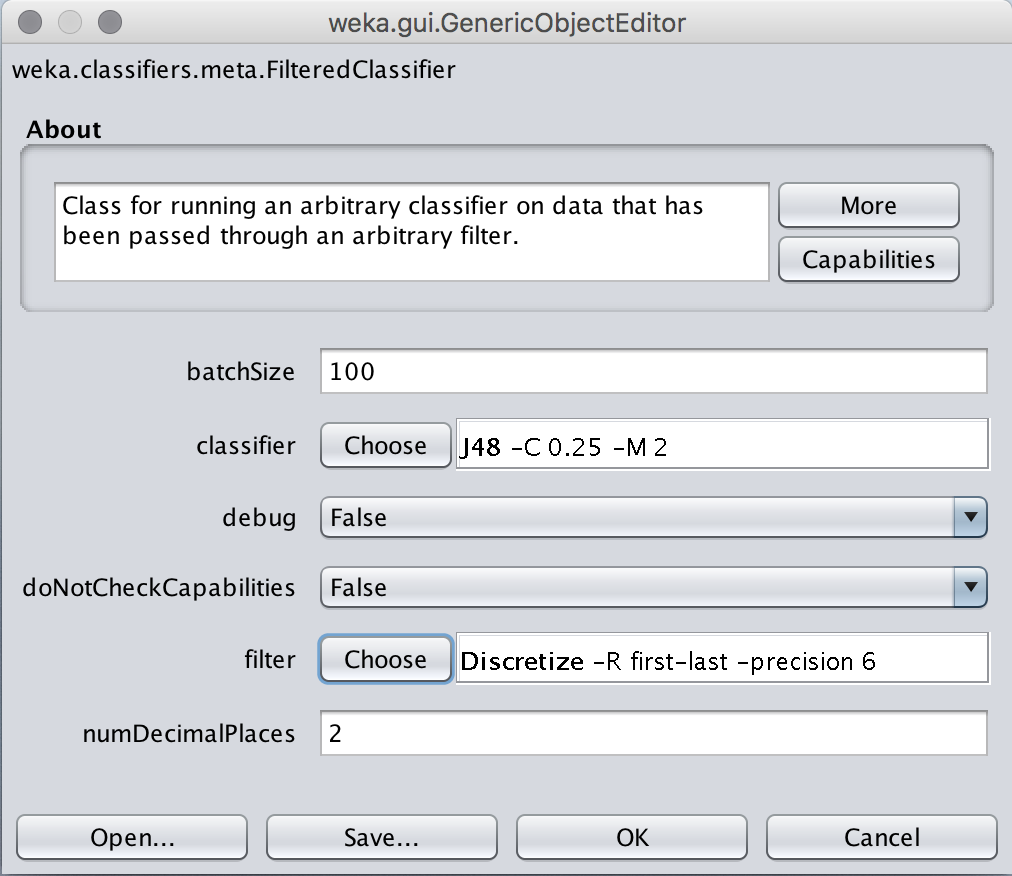
\includegraphics[width=0.45\textwidth]{images/B2_17a.png}}
\qquad
\subfloat[The menu of filters.]{\label{subfig:filtered_classifier_2}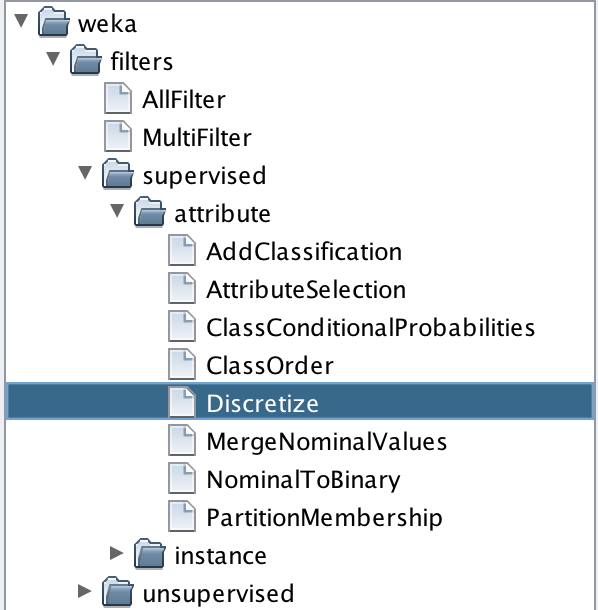
\includegraphics[width=0.45\textwidth]{images/B2_17b.png}}
\caption{\label{fig:filtered_classifier}Using WEKA's metalearner for discretization.}
\end{figure}

Because of popular demand, WEKA allows you to invoke supervised
filters as a preprocessing operation, just like unsupervised
filters. However, if you intend to use them for classification you
should adopt a different methodology. A \textit{metalearner} is
provided so that the process of building the filtering model becomes
part of the learning process. This filters the test data using the
filter that has been created from the training data. It is also useful
for some unsupervised filters. For example, in
\textit{StringToWordVector} the dictionary will be created from the
training data alone: words that are novel in the test data will be
discarded. To use a supervised filter in this way, invoke the
\textit{FilteredClassifier} metalearning scheme from the
\textit{meta} section of the menu displayed by the Classify panel's
Choose button. Figure~\ref{subfig:filtered_classifier_1} shows the
object editor for this metalearning scheme. With it you choose a
classifier and a filter. Figure~\ref{subfig:filtered_classifier_2}
shows the menu of filters.

Supervised filters, just like unsupervised ones, are divided into
attribute and instance filters.

\subsubsection{Supervised attribute filters}

\textit{Discretize}, highlighted in
Figure~\ref{fig:filtered_classifier}, uses the MDL method of
supervised discretization. You can specify a range of attributes or
force the discretized attribute to be binary. The class must be
nominal. By default Fayyad and Irani's (1993) criterion is used, but
Kononenko's method (1995) is an option.

There is a supervised version of the \textit{NominalToBinary} filter
that transforms all multivalued nominal attributes to binary ones. In
this version, the transformation depends on whether the class is
nominal or numeric. If nominal, the same method as before is used: an
attribute with \textit{k} values is transformed into \textit{k} binary
attributes. If the class is numeric, however, the method described in
used by the model tree learner M5' is applied. In either case the class itself is
not transformed.

\textit{ClassOrder} changes the ordering of the class values. The user
determines whether the new ordering is random or in ascending or
descending class frequency. This filter must not be used with the
\textit{FilteredClassifier} metalearning scheme!

\textit{AddClassification} adds to the data the predictions of a given
classifier, which can be either trained on the input dataset or loaded
from a file as a serialized object. New attributes can be added that
hold the predicted class value, the predicted probability distribution
(if the class is nominal), or a flag that indicates misclassified
instances (or, for numeric classes, the difference between the
predicted and actual class values).

\textit{AttributeSelection} applies a given attribute selection
technique in order to reduce the number of attributes in the data. The
user can choose which attribute or subset evaluator to use and combine
it with a search strategy in order to implement an attribute selection
method.

\textit{ClassConditionalProbabilities} converts the values of nominal
and numeric attributes into class conditional probability
estimates. For each original attribute $A$ converted, it creates as many
new attributes as there are class values, where the value of the new
attribute corresponding to class $C_k$ is $P(A | C_k)$. This is essentially the same as what the
naive Bayes classifier computes and, in fact, the implementation uses
naive Bayes internally. Like the unsupervised filters that merge
nominal values, this filter can help when dealing with nominal
attributes that have a large number of distinct values.

\subsubsection{Supervised instance filters}

There are four supervised instance filters. \textit{Resample} is like
the eponymous unsupervised instance filter except that it maintains
the class distribution in the subsample. Alternatively, it can be
configured to bias the class distribution towards a uniform
one. Sampling can be performed with (default) or without
replacement. \textit{SpreadSubsample} also produces a random
subsample, but the frequency difference between the rarest and the
most common class can be controlled---for example, you can specify at
most a 2 : 1 difference in class frequencies. You can also limit the
number of instances in any class by specifying an explicit maximum
count.

\textit{SMOTE} is another filter that samples the data and alters the
class distribution (Chawla et al., 2002). Like
\textit{SpreadSubsample}, it can be used to adjust the relative
frequency between minority and majority classes in the data---but it
takes care not to undersample majority classes and it oversamples the
minority class by creating synthetic instances using a
\textit{k}-nearest neighbor approach. The user can specify the
oversampling percentage and the number of neighbors to use when
creating synthetic instances.

Like the unsupervised instance filter \textit{RemoveFolds},
\textit{StratifiedRemoveFolds} outputs a specified cross-validation
fold for the dataset, except that this time the fold is stratified.

\section{Learning algorithms}

On the \textit{Classify} panel, when you select a learning algorithm
using the \textit{Choose} button the command-line version of the
classifier appears in the line beside the button, including the
parameters specified with minus signs. To change them, click that line
to get an appropriate object editor. The classifiers in WEKA are
divided into Bayesian classifiers, trees, rules, functions, lazy
classifiers and a final miscellaneous category. We describe them
briefly here, along with their parameters. To learn more, choose one
in the WEKA Explorer interface and examine its object editor. A
further kind of classifier, the metalearner, is described in the next
section.

\subsection{Bayesian classifiers}

\textit{NaiveBayes} implements the probabilistic Naive Bayes
classifier. \textit{NaiveBayesSimple} uses the normal distribution to
model numeric attributes. \textit{NaiveBayes} can use kernel density
estimators, which improve performance if the normality assumption is
grossly incorrect; it can also handle numeric attributes using
supervised discretization.

\begin{figure}[!p]
%\centering
\begin{mdframed}[innermargin=-1.5cm]
\begin{Verbatim}[fontsize=\scriptsize]
=== Run information ===

Scheme:       weka.classifiers.bayes.NaiveBayes 
Relation:     weather
Instances:    14
Attributes:   5
              outlook
              temperature
              humidity
              windy
              play
Test mode:    10-fold cross-validation

=== Classifier model (full training set) ===

Naive Bayes Classifier

                 Class
Attribute          yes      no
                (0.63)  (0.38)
===============================
outlook
  sunny             3.0     4.0
  overcast          5.0     1.0
  rainy             4.0     3.0
  [total]          12.0     8.0

temperature
  mean          72.9697 74.8364
  std. dev.      5.2304   7.384
  weight sum          9       5
  precision      1.9091  1.9091

humidity
  mean          78.8395 86.1111
  std. dev.      9.8023  9.2424
  weight sum          9       5
  precision      3.4444  3.4444

windy
  TRUE              4.0     4.0
  FALSE             7.0     3.0
  [total]          11.0     7.0



Time taken to build model: 0 seconds

=== Stratified cross-validation ===
=== Summary ===

Correctly Classified Instances           9               64.2857 %
Incorrectly Classified Instances         5               35.7143 %
Kappa statistic                          0.1026
Mean absolute error                      0.4649
Root mean squared error                  0.543 
Relative absolute error                 97.6254 %
Root relative squared error            110.051  %
Total Number of Instances               14     

=== Detailed Accuracy By Class ===

                 TP Rate  FP Rate  Precision  Recall   F-Measure  MCC      ROC Area  PRC Area  Class
                 0.889    0.800    0.667      0.889    0.762      0.122    0.444     0.633     yes
                 0.200    0.111    0.500      0.200    0.286      0.122    0.444     0.397     no
Weighted Avg.    0.643    0.554    0.607      0.643    0.592      0.122    0.444     0.548     

=== Confusion Matrix ===

 a b   <-- classified as
 8 1 | a = yes
 4 1 | b = no
\end{Verbatim}
\end{mdframed}
\caption{\label{fig:naive_bayes_output}Output of \textit{NaiveBayes} for the weather data.}
\end{figure}

Figure~\ref{fig:naive_bayes_output} shows the output of
\textit{NaiveBayes} on the weather data. The salient difference
between this and the output in Figure~\ref{fig:j48_output} of
\textit{J48} on the same data is that instead of a tree in textual
form, here the parameters of the \textit{Naive Bayes} model are
presented in a table. The first column shows attributes and the other
two show class values; entries are either frequency counts of nominal
values or parameters of normal distributions for numeric
attributes. For example, Figure~\ref{fig:naive_bayes_output} shows
that the mean temperature value for instances of class yes is 72.9697,
while for instances for which $windy = yes$ the values \textit{true}
and \textit{false} occur 4 and 7 times respectively. The grand total
of the yes and no counts for \textit{windy} is, surprisingly,
18---more than the 14 instances in the weather data (the situation for
\textit{outlook} is even worse, totaling 20). The reason is that
\textit{NaiveBayes} avoids zero frequencies by applying the Laplace
correction, which involves initializing each count to 1 rather than to
0.

\textit{NaiveBayesUpdateable} is an incremental version that processes
one instance at a time; it can use a kernel estimator but not
discretization. \textit{NaiveBayesMultinomial} implements the
multinomial Bayes classifier; \textit{NaiveBayesMultinomialUpdateable}
is an incremental version. \textit{NaiveBayesMultinomialText} is a
version of incremental multinomial naive Bayes that can work directly
on string attributes. It effectively performs the function of the
\textit{StringToWordVector} filter, minus the TF/IDF transformation,
on the fly.

\textit{BayesNet} learns Bayesian nets under the assumptions made in
Section 6.7: nominal attributes (numeric ones are prediscretized) and
no missing values (any such values are replaced globally). There are
four different algorithms for estimating the conditional probability
tables of the network. Search is done using the K2 or the TAN
algorithms, or more sophisticated methods based on hill-climbing,
simulated annealing, tabu search, and genetic algorithms. Optionally
search speed can be improved using AD trees. There are also two
algorithms that use conditional independence tests to learn the
structure of the network; alternatively, the network structure can be
loaded from an XML file. More details on the implementation of
Bayesian networks in WEKA can be found in Bouckaert (2004).

\begin{figure}[!th]
\centering
\subfloat[Default outpuit.]{\label{subfig:bayes_net_1}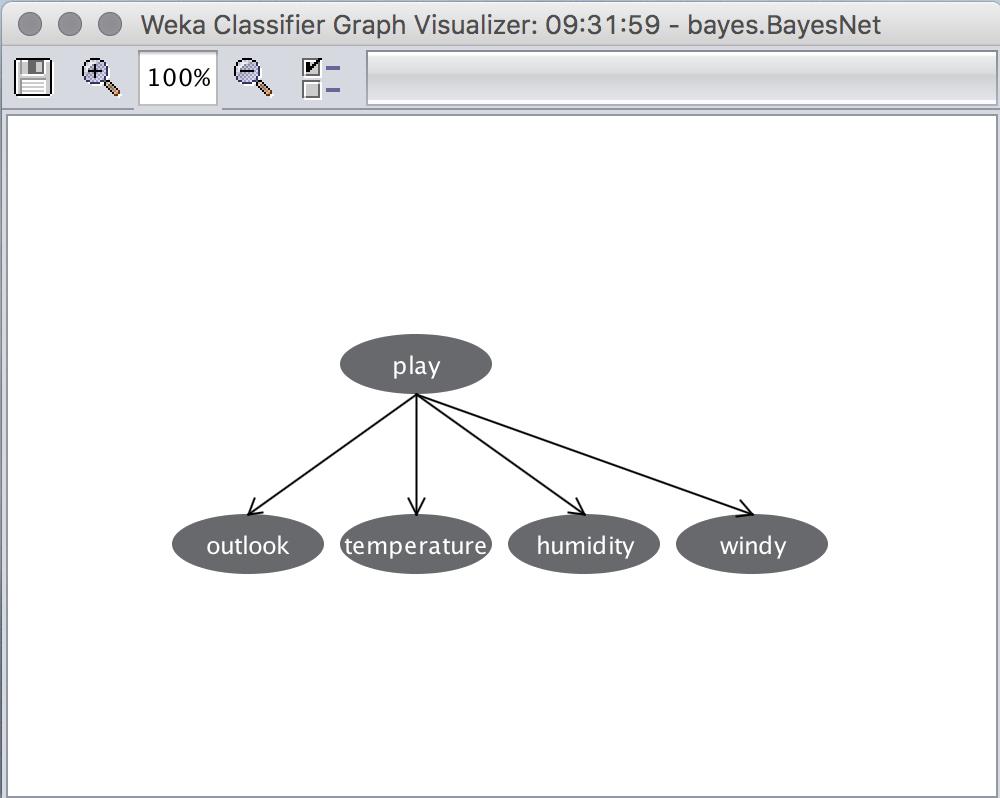
\includegraphics[width=0.45\textwidth]{images/B2_19a.png}}
\qquad
\subfloat[Maximum number of parents set to three in the search algorithm.]{\label{subfig:bayes_net_2}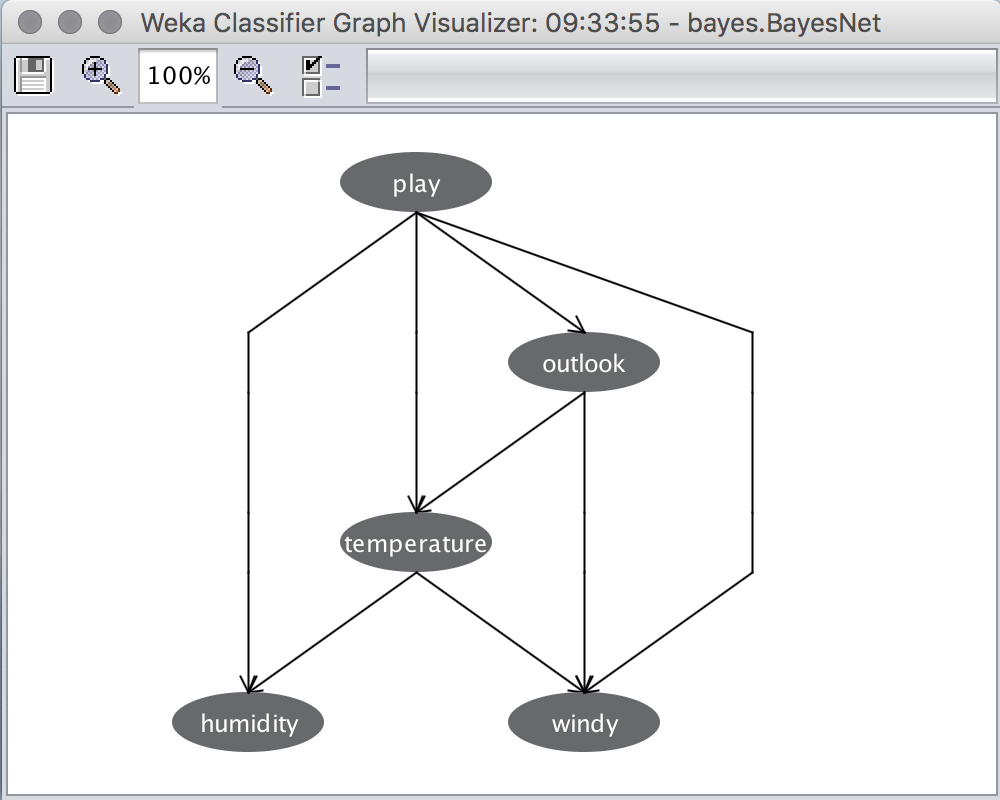
\includegraphics[width=0.45\textwidth]{images/B2_19b.png}}
\newline
\subfloat[The probability distribution table for the windy node in (b).]{\label{subfig:bayes_net_3}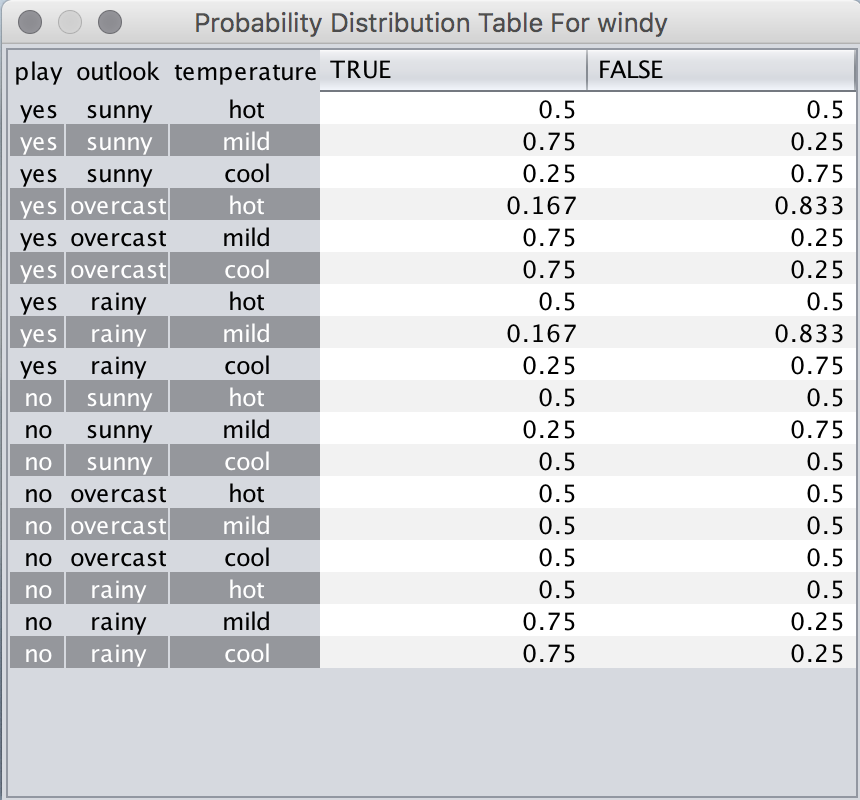
\includegraphics[width=0.45\textwidth]{images/B2_19c.png}}
\caption{\label{fig:weather}Visualizing a Bayesian network for the weather data (nominal version).}
\end{figure}

You can observe the network structure by right-clicking the history
item and selecting Visualize graph. Figure~\ref{subfig:bayes_net_1}
shows the graph for the nominal version of the weather data, which in
fact corresponds to the Naive Bayes result with all probabilities
conditioned on the class value. This is because the search algorithm
defaults to K2 with the maximum number of parents of a node set to
one. Reconfiguring this to three by clicking on K2 in the
configuration panel yields the more interesting network in
Figure~\ref{subfig:bayes_net_2}. Clicking on a node shows its
probability distribution---Figure~\ref{subfig:bayes_net_3} is obtained
by clicking on the windy node in Figure~\ref{subfig:bayes_net_2}.

\subsection{Trees}

\begin{figure}[!th]
\centering
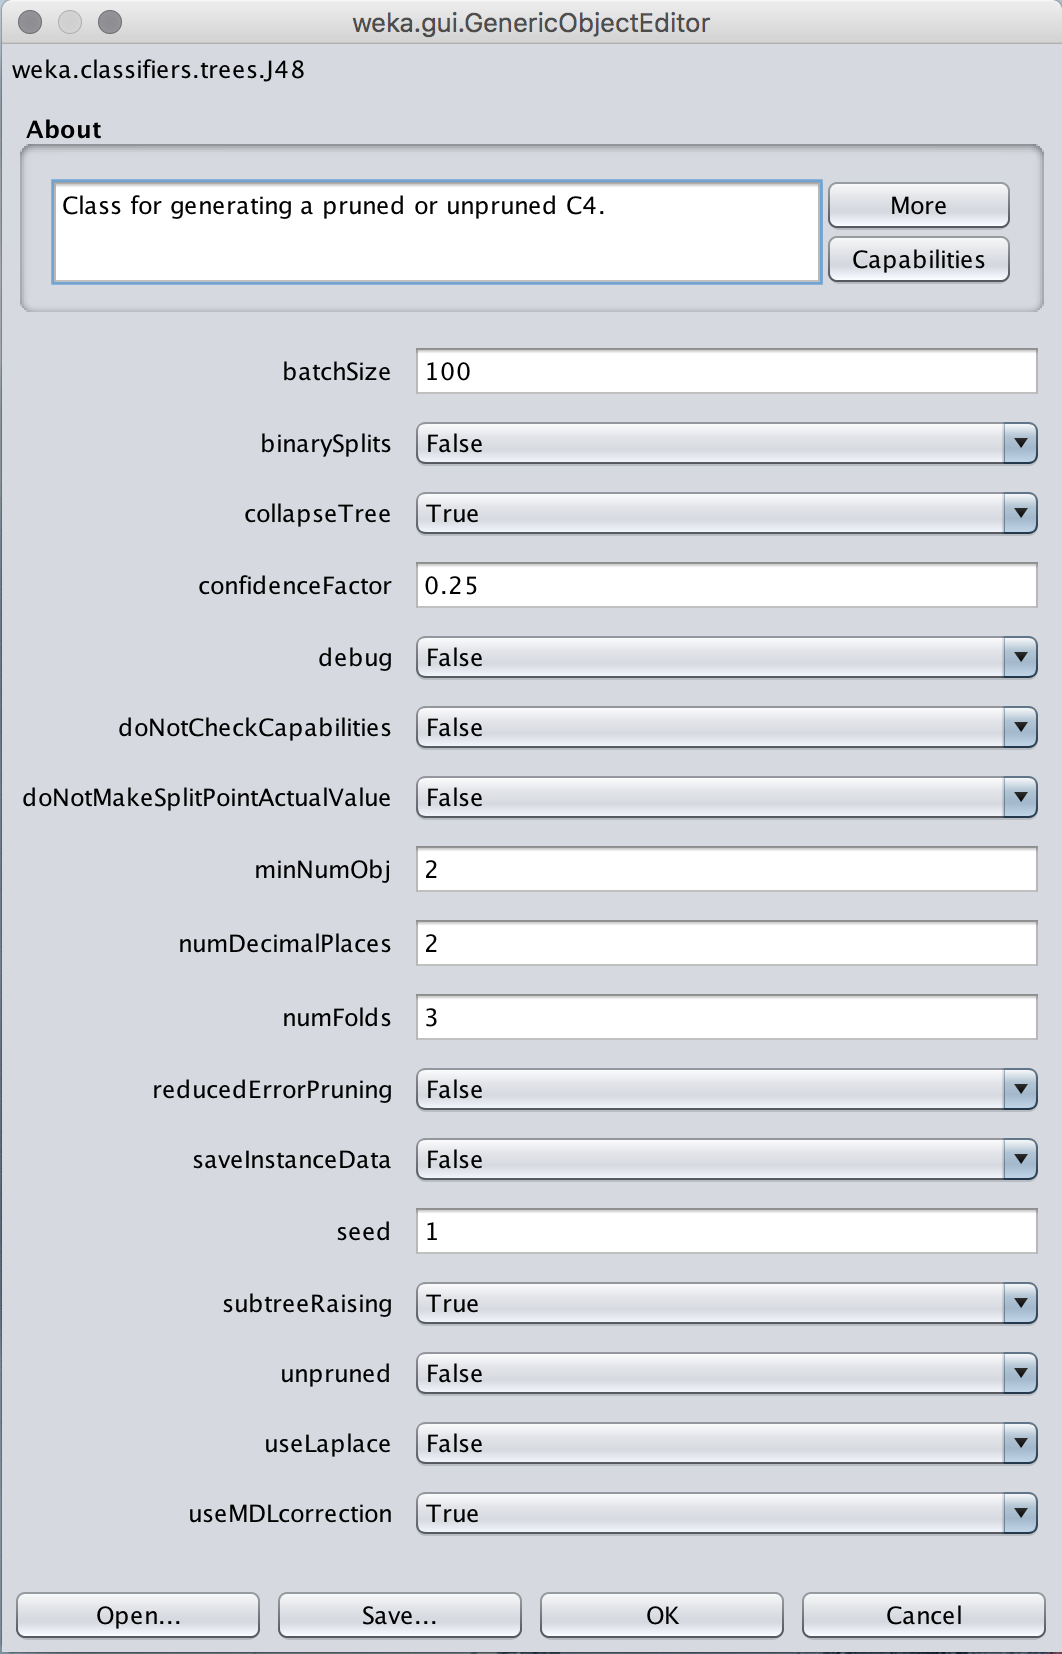
\includegraphics[width=0.6\textwidth]{images/B2_20.png}
\caption{Changing the parameters for J4.8.}
\label{fig:goe_j48}
\end{figure}

Of the tree classifiers in WEKA, we have already seen how to use J4.8,
which reimplements C4.5. To see the options, click the line beside the
\textit{Choose} button in Figure~\ref{subfig:j48_2} to bring up the
object editor in Figure~\ref{fig:goe_j48}. You can build a binary tree
instead of one with multiway branches. You can set the confidence
threshold for pruning (default 0.25), and the minimum number of
instances permissible at a leaf (default 2). Instead of standard C4.5
pruning you can choose reduced-error pruning. The \textit{numFolds}
parameter (default 3) determines the size of the pruning set: the data
is divided equally into that number of parts and the last one used for
pruning. When visualizing the tree it is nice to be able to consult
the original data points, which you can do if
\textit{saveInstanceData} has been turned on (it is off, or
\textit{False}, by default to reduce memory requirements). You can
suppress subtree raising, yielding a more efficient algorithm; force
the algorithm to use the unpruned tree instead of the pruned one; or
use Laplace smoothing for predicted probabilities.

\textit{DecisionStump}, designed for use with the boosting methods
described later, builds one-level binary decision trees for datasets
with a categorical or numeric class, dealing with missing values by
treating them as a separate value and extending a third branch from
the stump. Trees built by \textit{RandomTree} consider a given number of
random features at each node, performing no
pruning. \textit{RandomForest} constructs random forests by bagging
ensembles of random trees.

\textit{REPTree} builds a decision or regression tree using
information gain/variance reduction and prunes it using reduced-error
pruning. Optimized for speed, it only sorts values for numeric
attributes once. It deals with missing values
by splitting instances into pieces, as C4.5 does. You can set the
minimum number of instances per leaf, maximum tree depth (useful when
boosting trees), minimum proportion of training set variance for a
split (numeric classes only), and number of folds for pruning.

\textit{M5P} is the model tree learner M5$\prime$ described in Chapter 7 of the book.

\textit{LMT} builds logistic model trees. It can deal with binary and
multiclass target variables, numeric and nominal attributes, and
missing values. When fitting the logistic regression functions at a
node using the \textit{LogitBoost} algorithm, it uses cross-validation
to determine how many iterations to run just once and employs the same
number throughout the tree instead of cross-validating at every
node. This heuristic (which you can switch off) improves the run time
considerably, with little effect on accuracy. Alternatively, you can
set the number of boosting iterations to be used throughout the tree
manually, or use a fast heuristic based on the Akaike Information
Criterion instead of cross-validation. Weight trimming during the
boosting process can be used to further improve run time. Normally, it
is the misclassification error that cross-validation minimizes, but
the mean absolute error of the probability estimates can be chosen
instead. The splitting criterion can be based on C4.5's information
gain (the default) or on the LogitBoost residuals, striving to improve
the purity of the residuals. LMT employs the minimal cost-complexity
pruning mechanism to produce a compact tree structure.

\textit{HoeffdingTree} is an implementation of the incremental decision tree
algorithm algorithm described in Chapter 13 of the book. It offers options to
create splits based on information gain or the Gini index. Predictions
at the leaves of the tree can be made by either majority class or
naive Bayes models.

\subsection{Rules}

\textit{DecisionTable} builds a decision table classifier. It
evaluates feature subsets using best-first search and can use
cross-validation for evaluation (Kohavi 1995b). An option uses the
nearest-neighbor method to determine the class for each instance that
is not covered by a decision table entry, instead of the table's
global majority, based on the same set of features.

\begin{figure}[!p]
%\centering
\begin{mdframed}[innermargin=-1.5cm]
\begin{Verbatim}[fontsize=\scriptsize]
=== Run information ===

Scheme:       weka.classifiers.rules.OneR -B 6
Relation:     labor-neg-data
Instances:    57
Attributes:   17
              duration
              wage-increase-first-year
              wage-increase-second-year
              wage-increase-third-year
              cost-of-living-adjustment
              working-hours
              pension
              standby-pay
              shift-differential
              education-allowance
              statutory-holidays
              vacation
              longterm-disability-assistance
              contribution-to-dental-plan
              bereavement-assistance
              contribution-to-health-plan
              class
Test mode:    10-fold cross-validation

=== Classifier model (full training set) ===

wage-increase-first-year:
< 2.9-> bad
>= 2.9-> good
?-> good
(48/57 instances correct)


Time taken to build model: 0 seconds

=== Stratified cross-validation ===
=== Summary ===

Correctly Classified Instances          41               71.9298 %
Incorrectly Classified Instances        16               28.0702 %
Kappa statistic                          0.3382
Mean absolute error                      0.2807
Root mean squared error                  0.5298
Relative absolute error                 61.3628 %
Root relative squared error            110.9627 %
Total Number of Instances               57     

=== Detailed Accuracy By Class ===

                 TP Rate  FP Rate  Precision  Recall   F-Measure  MCC      ROC Area  PRC Area  Class
                 0.450    0.135    0.643      0.450    0.529      0.349    0.657     0.482     bad
                 0.865    0.550    0.744      0.865    0.800      0.349    0.657     0.731     good
Weighted Avg.    0.719    0.404    0.709      0.719    0.705      0.349    0.657     0.644     

=== Confusion Matrix ===

  a  b   <-- classified as
  9 11 |  a = bad
  5 32 |  b = good
\end{Verbatim}
\end{mdframed}
\caption{\label{fig:oneR_output}Output of \textit{OneR} for the labor negotiations data.}
\end{figure}

\textit{OneR} is the 1R classifier with one parameter: the minimum
bucket size for discretization. Figure~\ref{fig:oneR_output} shows its
output for the labor negotiations data. The Classifier model part
shows that wage-increase-first-year has been identified as the basis
of the rule produced, with a split at the value 2.9 dividing bad
outcomes from good ones (the class is also good if the value of that
attribute is missing). Beneath the rules the fraction of training
instances correctly classified by the rules is given in parentheses.

\begin{figure}[!p]
%\centering
\begin{mdframed}[innermargin=-1.5cm]
\begin{Verbatim}[fontsize=\scriptsize]
=== Run information ===

Scheme:       weka.classifiers.rules.PART -M 2 -C 0.25 -Q 1
Relation:     labor-neg-data
Instances:    57
Attributes:   17
              duration
              wage-increase-first-year
              wage-increase-second-year
              wage-increase-third-year
              cost-of-living-adjustment
              working-hours
              pension
              standby-pay
              shift-differential
              education-allowance
              statutory-holidays
              vacation
              longterm-disability-assistance
              contribution-to-dental-plan
              bereavement-assistance
              contribution-to-health-plan
              class
Test mode:    10-fold cross-validation

=== Classifier model (full training set) ===

PART decision list
------------------

wage-increase-first-year > 2.5 AND
longterm-disability-assistance = yes AND
statutory-holidays > 10: good (25.67)

wage-increase-first-year <= 4 AND
working-hours > 36: bad (19.4/1.58)

: good (11.93/2.18)

Number of Rules  : 3


Time taken to build model: 0.01 seconds

=== Stratified cross-validation ===
=== Summary ===

Correctly Classified Instances          45               78.9474 %
Incorrectly Classified Instances        12               21.0526 %
Kappa statistic                          0.5378
Mean absolute error                      0.2884
Root mean squared error                  0.4339
Relative absolute error                 63.0507 %
Root relative squared error             90.8836 %
Total Number of Instances               57     

=== Detailed Accuracy By Class ===

                 TP Rate  FP Rate  Precision  Recall   F-Measure  MCC      ROC Area  PRC Area  Class
                 0.700    0.162    0.700      0.700    0.700      0.538    0.726     0.613     bad
                 0.838    0.300    0.838      0.838    0.838      0.538    0.726     0.758     good
Weighted Avg.    0.789    0.252    0.789      0.789    0.789      0.538    0.726     0.707     

=== Confusion Matrix ===

  a  b   <-- classified as
 14  6 |  a = bad
  6 31 |  b = good
\end{Verbatim}
\end{mdframed}
\caption{\label{fig:part_output}Output of \textit{Part} for the labor negotiations data.}
\end{figure}

\textit{Part} obtains rules from partial decision trees. It builds the
tree using C4.5's heuristics with the same user-defined parameters as
J4.8. Figure~\ref{fig:part_output} shows the output of Part for the
labor negotiations data. Three rules are found, and are intended to be
processed in order, the prediction generated for any test instance
being the outcome of the first rule that fires. The last, ``catch-all,''
rule will always fire if no other rule fires. As with J48, the numbers in parentheses that
follow each rule give the number of instances that are covered by the
rule followed by the number that are misclassified (if any).

\textit{M5Rules} obtains regression rules from model trees built using
M5'. \textit{Ridor} learns rules with exceptions by generating the
default rule, using incremental reduced-error pruning to find
exceptions with the smallest error rate, finding the best exceptions
for each exception, and iterating.

\textit{JRip} implements Ripper algorithm, including heuristic global
optimization of the rule set (Cohen 1995). \textit{NNge} is a
nearest-neighbor method for generating rules using nonnested
generalized exemplars.

\subsection{Functions}

\begin{figure}[!hp]
%\centering
\begin{mdframed}[innermargin=-1.5cm]
\begin{Verbatim}[fontsize=\footnotesize]
=== Run information ===

Scheme:       weka.classifiers.functions.SimpleLinearRegression 
Relation:     cpu
Instances:    209
Attributes:   7
              MYCT
              MMIN
              MMAX
              CACH
              CHMIN
              CHMAX
              class
Test mode:    10-fold cross-validation

=== Classifier model (full training set) ===

Linear regression on MMAX

0.01 * MMAX - 34

Predicting 0 if attribute value is missing.


Time taken to build model: 0 seconds

=== Cross-validation ===
=== Summary ===

Correlation coefficient                  0.7844
Mean absolute error                     53.8054
Root mean squared error                 99.5674
Relative absolute error                 55.908  %
Root relative squared error             61.8997 %
Total Number of Instances              209 
\end{Verbatim}
\end{mdframed}
\caption{\label{fig:simple_linear_regression_output}Output of \textit{SimpleLinearRegression} on the CPU performance data.}
\end{figure}

Algorithms that fall into the \textit{functions} category include an
assorted group of classifiers that can be written down as mathematical
equations in a reasonably natural way. Other methods, such as decision
trees and rules, cannot (there are exceptions: Naive Bayes has a
simple mathematical formulation). Four of them implement linear
regression. \textit{SimpleLinearRegression} learns a linear regression
model based on a single attribute---it chooses the one that yields the
smallest squared error. Missing values and nonnumeric attributes are
not allowed. Figure~\ref{fig:simple_linear_regression_output} shows
the output of \textit{SimpleLinearRegression} for the CPU performance
data. The attribute that has the smallest squared error in this case
is \textit{MMAX}.

\textit{LinearRegression} performs least-squares multiple
linear regression including attribute selection,
either greedily using backward elimination or by building a full model
from all attributes and dropping terms one by one in decreasing order
of their standardized coefficients until a stopping criteria is
reached. Both methods use a version of the AIC termination
criterion. Attribute selection can be turned off. The implementation has two further refinements: a heuristic
mechanism for detecting collinear attributes (which can be turned off)
and a ridge parameter that stabilizes degenerate cases and can reduce
overfitting by penalizing large coefficients. Technically,
\textit{LinearRegression} implements ridge regression.

\textit{SMO} implements the sequential minimal optimization algorithm for
training a support vector classifier (Platt, 1998; Keerthi
et al., 2001), using kernel
functions such as polynomial or Gaussian kernels. Missing values are replaced globally, nominal
attributes are transformed into binary ones, and attributes are
normalized by default---note that the coefficients in the output are
based on the normalized data. Normalization can be turned off, or the
input standardized to zero mean and unit variance. Pairwise
classification is used for multiclass problems. Logistic regression
models can be fitted to the support vector machine output to obtain
probability estimates. In the multiclass case the predicted
probabilities will be combined using pairwise coupling (Hastie and
Tibshirani, 1998). When working with sparse instances, turn
normalization off for faster operation.

\begin{figure}[!p]
%\centering
\begin{mdframed}[innermargin=-1.0cm]
\begin{Verbatim}[fontsize=\tiny]
=== Run information ===

Scheme:       weka.classifiers.functions.SMO -C 1.0 -L 0.001 -P 1.0E-12 -N 0 -V -1 -W 1 
              -K ``weka.classifiers.functions.supportVector.PolyKernel -E 1.0 -C 250007'' 
              -calibrator ``weka.classifiers.functions.Logistic -R 1.0E-8 -M -1 -num-decimal-places 4''
Relation:     iris
Instances:    150
Attributes:   5
              sepallength
              sepalwidth
              petallength
              petalwidth
              class
Test mode:    10-fold cross-validation

=== Classifier model (full training set) ===

SMO

Kernel used:
  Linear Kernel: K(x,y) = <x,y>

Classifier for classes: Iris-setosa, Iris-versicolor

BinarySMO
Machine linear: showing attribute weights, not support vectors.

         0.6829 * (normalized) sepallength
 +      -1.523  * (normalized) sepalwidth
 +       2.2034 * (normalized) petallength
 +       1.9272 * (normalized) petalwidth
 -       0.7091

Number of kernel evaluations: 352 (70.32% cached)

Classifier for classes: Iris-setosa, Iris-virginica

BinarySMO
Machine linear: showing attribute weights, not support vectors.

         0.5886 * (normalized) sepallength
 +      -0.5782 * (normalized) sepalwidth
 +       1.6429 * (normalized) petallength
 +       1.4777 * (normalized) petalwidth
 -       1.1668

Number of kernel evaluations: 284 (68.996% cached)

Classifier for classes: Iris-versicolor, Iris-virginica

BinarySMO
Machine linear: showing attribute weights, not support vectors.

         0.3176 * (normalized) sepallength
 +      -0.863  * (normalized) sepalwidth
 +       3.0543 * (normalized) petallength
 +       4.0815 * (normalized) petalwidth
 -       4.5924

Number of kernel evaluations: 453 (61.381% cached)

Time taken to build model: 0.03 seconds

=== Stratified cross-validation ===
=== Summary ===

Correctly Classified Instances         144               96      %
Incorrectly Classified Instances         6                4      %
Kappa statistic                          0.94  
Mean absolute error                      0.2311
Root mean squared error                  0.288 
Relative absolute error                 52      %
Root relative squared error             61.101  %
Total Number of Instances              150     

=== Detailed Accuracy By Class ===

                 TP Rate  FP Rate  Precision  Recall   F-Measure  MCC      ROC Area  PRC Area  Class
                 1.000    0.000    1.000      1.000    1.000      1.000    1.000     1.000     Iris-setosa
                 0.980    0.050    0.907      0.980    0.942      0.913    0.965     0.896     Iris-versicolor
                 0.900    0.010    0.978      0.900    0.938      0.910    0.970     0.930     Iris-virginica
Weighted Avg.    0.960    0.020    0.962      0.960    0.960      0.941    0.978     0.942     

=== Confusion Matrix ===

  a  b  c   <-- classified as
 50  0  0 |  a = Iris-setosa
  0 49  1 |  b = Iris-versicolor
  0  5 45 |  c = Iris-virginica
\end{Verbatim}
\end{mdframed}
\caption{\label{fig:smo_output}Output of \textit{SMO} on the iris data.}
\end{figure}

\begin{figure}[!p]
%\centering
\begin{mdframed}[innermargin=-1.0cm]
\begin{Verbatim}[fontsize=\tiny]
=== Run information ===

Scheme:       weka.classifiers.functions.SMO -C 1.0 -L 0.001 -P 1.0E-12 -N 0 -V -1 -W 1 
              -K ``weka.classifiers.functions.supportVector.PolyKernel -E 2.0 -C 250007'' 
              -calibrator ``weka.classifiers.functions.Logistic -R 1.0E-8 -M -1 -num-decimal-places 4''
Relation:     iris
Instances:    150
Attributes:   5
              sepallength
              sepalwidth
              petallength
              petalwidth
              class
Test mode:    10-fold cross-validation

=== Classifier model (full training set) ===

SMO

Kernel used:
  Poly Kernel: K(x,y) = <x,y>^2.0

Classifier for classes: Iris-setosa, Iris-versicolor

BinarySMO

      1      * <0.333333 0.166667 0.457627 0.375 > * X]
 -       1      * <0.222222 0.541667 0.118644 0.166667 > * X]
 -       1      * <0.138889 0.416667 0.067797 0.083333 > * X]
 -       1      * <0.166667 0.416667 0.067797 0.041667 > * X]
 +       1      * <0.222222 0.208333 0.338983 0.416667 > * X]
 -       1      * <0.055556 0.125 0.050847 0.083333 > * X]
 -       1      * <0.027778 0.375 0.067797 0.041667 > * X]
 +       1      * <0.166667 0.166667 0.389831 0.375 > * X]
 +       1      * <0.361111 0.208333 0.491525 0.416667 > * X]
 +       1      * <0.194444 0 0.423729 0.375 > * X]
 -       1      * <0.194444 0.416667 0.101695 0.041667 > * X]
 -       1      * <0.138889 0.458333 0.101695 0.041667 > * X]
 +       1      * <0.194444 0.125 0.389831 0.375 > * X]
 +       0.3697 * <0.361111 0.375 0.440678 0.5 > * X]
 -       0.4599 * <0.138889 0.416667 0.067797 0 > * X]
 -       0.9098 * <0.194444 0.625 0.101695 0.208333 > * X]
 +       1      * <0.333333 0.166667 0.474576 0.416667 > * X]
 +       1      * <0.388889 0.25 0.423729 0.375 > * X]
 -       0.8085

Number of support vectors: 18

Number of kernel evaluations: 2416 (72.564% cached)

Classifier for classes: Iris-setosa, Iris-virginica

BinarySMO
      1      * <0.166667 0.208333 0.59322 0.666667 > * X]
 -       0.856  * <0.055556 0.125 0.050847 0.083333 > * X]
 +       0.1315 * <0.555556 0.333333 0.694915 0.583333 > * X]
 -       1      * <0.222222 0.541667 0.118644 0.166667 > * X]
 +       1      * <0.472222 0.083333 0.677966 0.583333 > * X]
 -       0.2756 * <0.194444 0.625 0.101695 0.208333 > * X]
 -       1.0183

Number of support vectors: 6

Number of kernel evaluations: 1364 (60.726% cached)

Classifier for classes: Iris-versicolor, Iris-virginica

BinarySMO
      1      * <0.555556 0.208333 0.677966 0.75 > * X]
 -       1      * <0.305556 0.416667 0.59322 0.583333 > * X]
 -       1      * <0.666667 0.458333 0.627119 0.583333 > * X]
 -       1      * <0.472222 0.583333 0.59322 0.625 > * X]
 +       1      * <0.444444 0.416667 0.694915 0.708333 > * X]
 -       1      * <0.527778 0.083333 0.59322 0.583333 > * X]
 +       1      * <0.416667 0.291667 0.694915 0.75 > * X]
 -       1      * <0.472222 0.291667 0.694915 0.625 > * X]
 +       0.4559 * <0.555556 0.375 0.779661 0.708333 > * X]
 -       1      * <0.666667 0.416667 0.677966 0.666667 > * X]
 +       1      * <0.611111 0.416667 0.762712 0.708333 > * X]
 -       1      * <0.5 0.375 0.627119 0.541667 > * X]
 -       1      * <0.722222 0.458333 0.661017 0.583333 > * X]
 +       1      * <0.472222 0.083333 0.677966 0.583333 > * X]
 +       1      * <0.583333 0.458333 0.762712 0.708333 > * X]
 +       1      * <0.611111 0.5 0.694915 0.791667 > * X]
 +       1      * <0.5 0.416667 0.661017 0.708333 > * X]
 -       1      * <0.694444 0.333333 0.644068 0.541667 > * X]
 -       1      * <0.5 0.416667 0.610169 0.541667 > * X]
 +       1      * <0.416667 0.291667 0.694915 0.75 > * X]
 +       1      * <0.527778 0.333333 0.644068 0.708333 > * X]
 -       1      * <0.444444 0.5 0.644068 0.708333 > * X]
 +       1      * <0.5 0.25 0.779661 0.541667 > * X]
 +       1      * <0.555556 0.291667 0.661017 0.708333 > * X]
 +       1      * <0.361111 0.333333 0.661017 0.791667 > * X]
 -       1      * <0.555556 0.208333 0.661017 0.583333 > * X]
 -       0.4559 * <0.555556 0.125 0.576271 0.5 > * X]
 +       1      * <0.555556 0.333333 0.694915 0.583333 > * X]
 +       1      * <0.166667 0.208333 0.59322 0.666667 > * X]
 +       1      * <0.805556 0.416667 0.813559 0.625 > * X]
 -       1      * <0.555556 0.541667 0.627119 0.625 > * X]
 +       1      * <0.472222 0.416667 0.644068 0.708333 > * X]
 -       1      * <0.361111 0.416667 0.59322 0.583333 > * X]
 -       1      * <0.583333 0.5 0.59322 0.583333 > * X]
 -       1      * <0.472222 0.375 0.59322 0.583333 > * X]
 -       1      * <0.611111 0.333333 0.610169 0.583333 > * X]
 -       3.5378

Number of support vectors: 36

Number of kernel evaluations: 3524 (66.711% cached)

Time taken to build model: 0.01 seconds
\end{Verbatim}
\end{mdframed}
\caption{\label{fig:smo_nonlinear_output}Output of \textit{SMO} with a nonlinear kernel on the iris data.}
\end{figure}

\begin{figure}[!th]
%\centering
\begin{mdframed}[innermargin=-1.0cm]
\begin{Verbatim}[fontsize=\tiny]
=== Stratified cross-validation ===
=== Summary ===

Correctly Classified Instances         144               96      %
Incorrectly Classified Instances         6                4      %
Kappa statistic                          0.94  
Mean absolute error                      0.2311
Root mean squared error                  0.288 
Relative absolute error                 52      %
Root relative squared error             61.101  %
Total Number of Instances              150     

=== Detailed Accuracy By Class ===

                 TP Rate  FP Rate  Precision  Recall   F-Measure  MCC      ROC Area  PRC Area  Class
                 1.000    0.000    1.000      1.000    1.000      1.000    1.000     1.000     Iris-setosa
                 0.940    0.030    0.940      0.940    0.940      0.910    0.955     0.904     Iris-versicolor
                 0.940    0.030    0.940      0.940    0.940      0.910    0.972     0.916     Iris-virginica
Weighted Avg.    0.960    0.020    0.960      0.960    0.960      0.940    0.976     0.940     

=== Confusion Matrix ===

  a  b  c   <-- classified as
 50  0  0 |  a = Iris-setosa
  0 47  3 |  b = Iris-versicolor
  0  3 47 |  c = Iris-virginica
\end{Verbatim}
\end{mdframed}
\caption{\label{fig:smo_nonlinear_cont} Output of \textit{SMO} with a nonlinear kernel on the iris data, cont'd.}
\end{figure}

Figure~\ref{fig:smo_output} shows the output of \textit{SMO} on the
iris data. A polynomial kernel with an exponent of 1 has been used,
making the model a linear support vector machine. Since the iris data
contains three class values, three binary SMO models have been
output---one hyperplane to separate each possible pair of class
values. Furthermore, since the machine is linear, the hyperplanes are
expressed as functions of the attribute values in the original (albeit
normalized) space. Figures~\ref{fig:smo_nonlinear_output} and~\ref{fig:smo_nonlinear_cont} show the result when the exponent of the
polynomial kernel is set to 2, making the support vector machine
nonlinear. There are three binary SMO models as before, but this time
the classifiers are expressed as functions of the support
vectors. Each support vector is shown enclosed in angle brackets,
along with the value of its coefficient $\alpha$. The value of the
offset parameter, $b$, is shown
as the last component of each function.

\textit{SMOreg} implements the sequential minimal optimization algorithm for
learning a support vector regression model (Smola and Schölkopf,
1998).

\textit{VotedPerceptron} is the voted perceptron
algorithm. \textit{Winnow} modifies the basic perceptron to use
multiplicative updates. The implementation allows for a second
multiplier $\beta$---different from $1/\alpha$---to be used, which
makes the algorithm slightly more flexible than the version of
balanced Winnow discussed in the book.

\textit{GaussianProcesses} implements the Bayesian Gaussian process
technique for non-linear regression. Users can specify the kernel
function, along with a ``noise'' regularization parameter for
controlling the closeness of fit. They can choose to have the training
data normalized or standardized before learning the regression. For
point estimates, this method is equivalent to kernel ridge regression.

\textit{SGD} implements stochastic gradient descent learning of linear
models. Models can be learned in either a batch or incremental
fashion. The loss function chosen determines the type of model
learned. Available loss functions include the hinge loss (linear
support vector classifier), log loss (logistic regression), squared
loss (least squares linear regression), epsilon-insensitive loss
(support vector regression) and Huber loss (robust
regression). \textit{SGDText}, like
\textit{NaiveBayesMultinomialText}, is a version that is designed for
text classification and can operate directly on string
attributes. \textit{SGDText} is limited to just the hinge and log
loss.

\textit{SimpleLogistic} builds logistic regression models, fitting
them using LogitBoost with simple regression functions as base
learners and determining how many iterations to perform using
cross-validation---which supports automatic attribute
selection. \textit{SimpleLogistic} generates a degenerate logistic
model tree comprising a single node, and supports the options given
earlier for \textit{LMT}.

\begin{figure}[!th]
%\centering
\begin{mdframed}[innermargin=-1.0cm]
\begin{Verbatim}[fontsize=\tiny]
=== Run information ===

Scheme:       weka.classifiers.functions.Logistic -R 1.0E-8 -M -1 -num-decimal-places 4
Relation:     iris
Instances:    150
Attributes:   5
              sepallength
              sepalwidth
              petallength
              petalwidth
              class
Test mode:    10-fold cross-validation

=== Classifier model (full training set) ===

Logistic Regression with ridge parameter of 1.0E-8
Coefficients...
                         Class
Variable           Iris-setosa  Iris-versicolor
===============================================
sepallength            21.8065           2.4652
sepalwidth              4.5648           6.6809
petallength           -26.3083          -9.4293
petalwidth             -43.887         -18.2859
Intercept               8.1743           42.637


Odds Ratios...
                         Class
Variable           Iris-setosa  Iris-versicolor
===============================================
sepallength    2954196659.8892          11.7653
sepalwidth             96.0426         797.0304
petallength                  0           0.0001
petalwidth                   0                0


Time taken to build model: 0.01 seconds

=== Stratified cross-validation ===
=== Summary ===

Correctly Classified Instances         144               96      %
Incorrectly Classified Instances         6                4      %
Kappa statistic                          0.94  
Mean absolute error                      0.0287
Root mean squared error                  0.1424
Relative absolute error                  6.456  %
Root relative squared error             30.2139 %
Total Number of Instances              150     

=== Detailed Accuracy By Class ===

                 TP Rate  FP Rate  Precision  Recall   F-Measure  MCC      ROC Area  PRC Area  Class
                 1.000    0.000    1.000      1.000    1.000      1.000    1.000     1.000     Iris-setosa
                 0.920    0.020    0.958      0.920    0.939      0.910    0.970     0.933     Iris-versicolor
                 0.960    0.040    0.923      0.960    0.941      0.911    0.975     0.933     Iris-virginica
Weighted Avg.    0.960    0.020    0.960      0.960    0.960      0.940    0.982     0.955     

=== Confusion Matrix ===

  a  b  c   <-- classified as
 50  0  0 |  a = Iris-setosa
  0 46  4 |  b = Iris-versicolor
  0  2 48 |  c = Iris-virginica
\end{Verbatim}
\end{mdframed}
\caption{\label{fig:logistic_output}Output of \textit{Logistic} for the iris data.}
\end{figure}

\textit{Logistic} is an alternative implementation for building and
using a multinomial logistic regression model with a ridge estimator
to guard against overfitting by penalizing large coefficients, based
on work by le Cessie and van Houwelingen
(1992). Figure~\ref{fig:logistic_output} shows its output on the iris
data. The coefficients of the regression functions are shown in
tabular form, one for each class value except for the last
class. Given $m$ input attributes and $k$ classes, the probability
predicted for class $j$ (with the exception of the last class) is given
by\newline

$P(j|a_1,a_2,...,a_m)=\frac{exp(w^j_0+w^j_1a_1+w^j_2a_2+...+w^j_ma_m)}{1 + \sum_{j=1}^{k-1}exp(w^j_0+w^j_1a_1+w^j_2a_2+...+w^j_ma_m)}$\newline

where $w^j_0$ is the intercept term for class $j$. The probability of the last class $k$ is given by\newline

$1-\sum_{j=1}^{k-1}P(j|a_1,a_2,...,a_m)$\newline

Beneath the table of regression coefficients is a second table giving
an estimate of the odds ratio for each input attribute and class
value. For a given attribute, this value gives an indication of its
influence on the class when the values of the other attributes are
held fixed.

\subsection{Neural networks}

\begin{figure}[!th]
\centering
\subfloat[Beginning the process of editing the network to add a second hidden layer.]{\label{subfig:mlp_editor_1}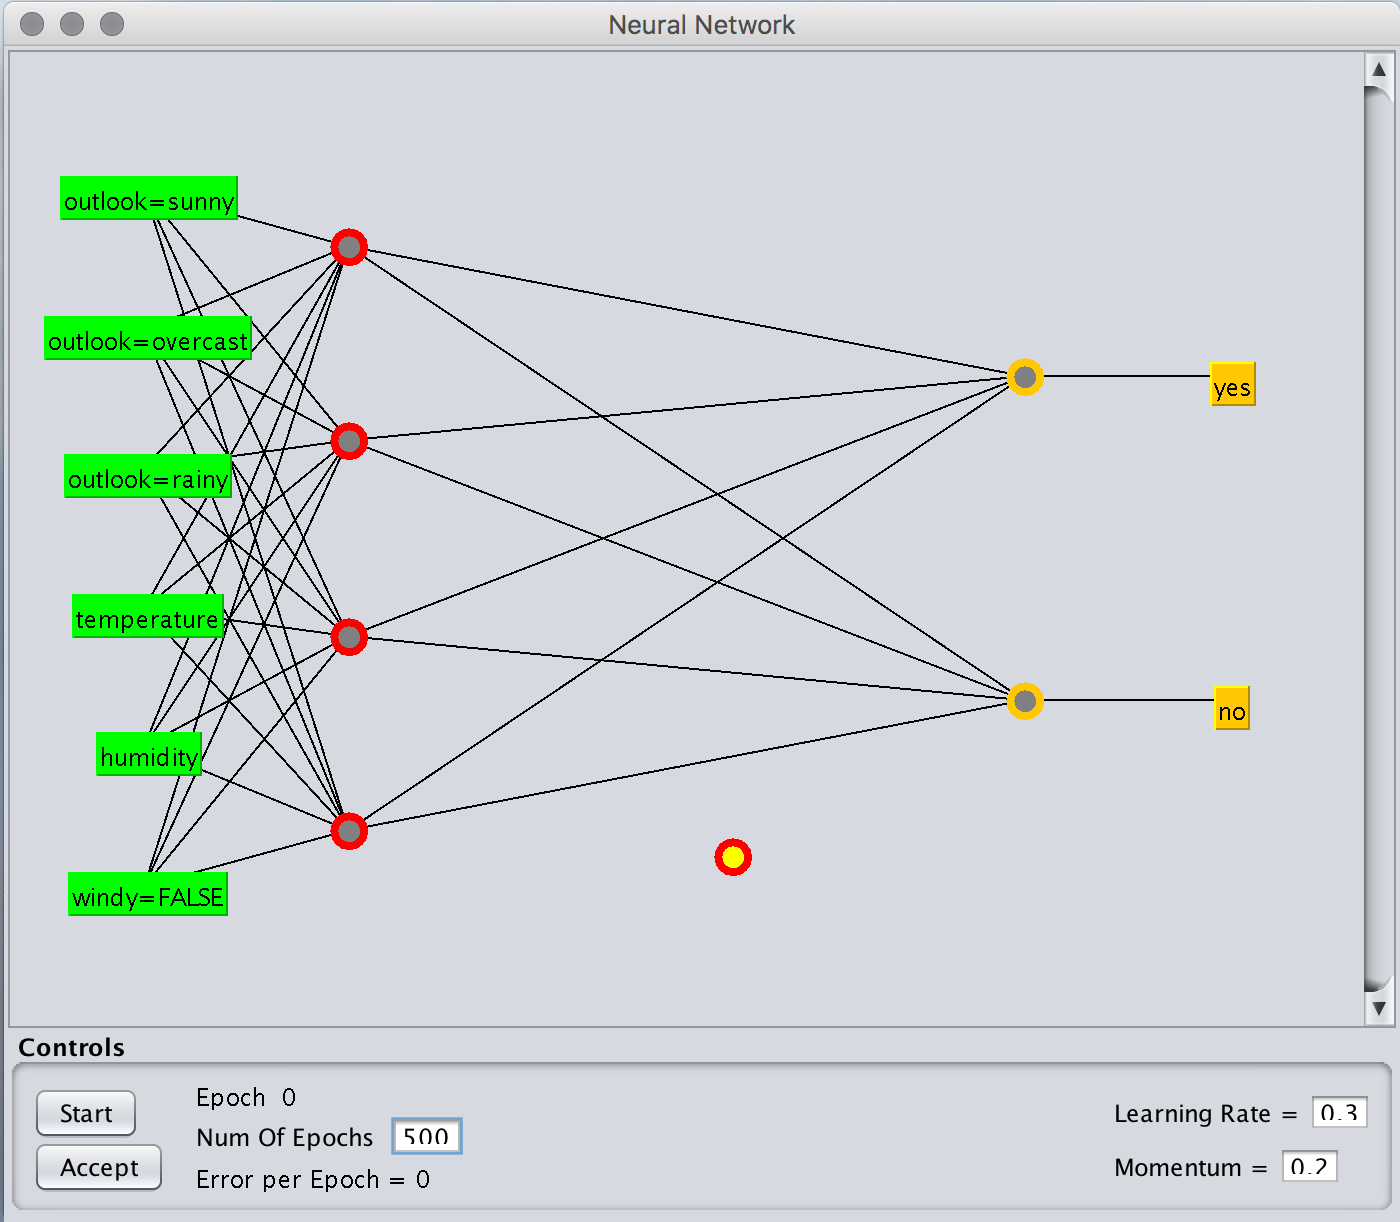
\includegraphics[width=0.75\textwidth]{images/B2_27a.png}}
\qquad
\subfloat[The finished network with two hidden layers.]{\label{subfig:mlp_editor_2}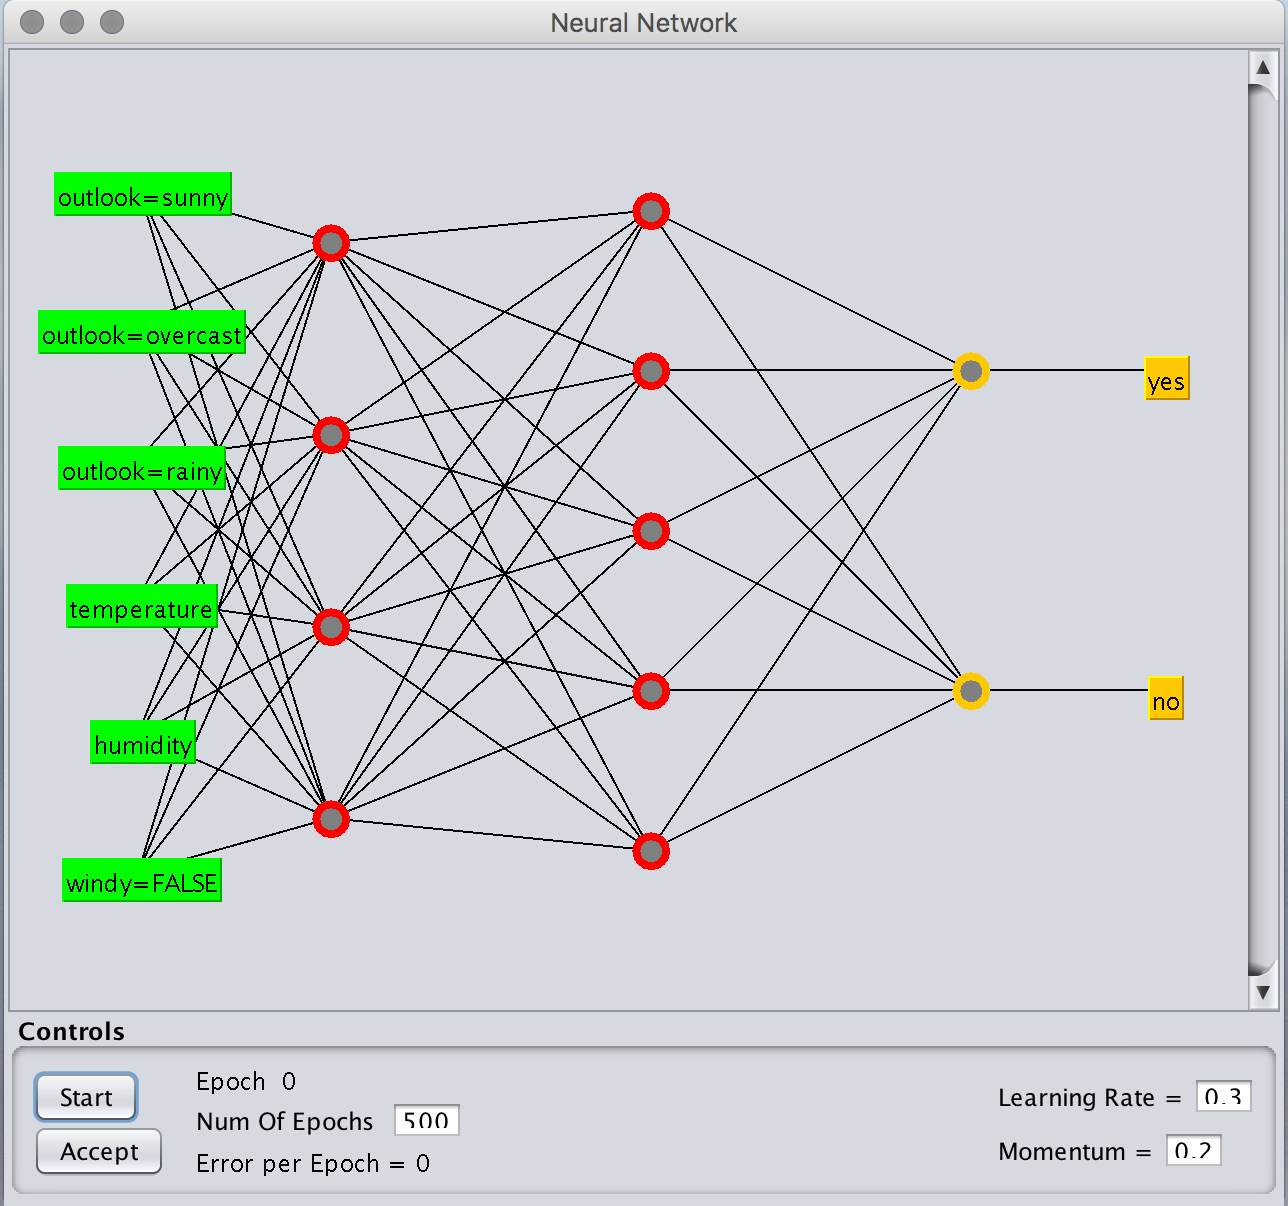
\includegraphics[width=0.75\textwidth]{images/B2_27b.png}}
\caption{\label{fig:mlp_editor}Using WEKA's neural-network graphical user interface.}
\end{figure}

\textit{MultilayerPerceptron} is a neural network that is trained using
back propagation. Although listed under functions, it differs from the
other schemes because it has its own user interface. If you load up
the numeric version of the weather data, invoke
\textit{MultilayerPerceptron}, set \textit{GUI} to \textit{True} in
its object editor, and run the network by clicking \textit{Start} on
the \textit{Classify} panel, the diagram in
Figure~\ref{fig:mlp_editor} appears in a separate window. This network
has three layers: an input layer on the left with one rectangular box
for each attribute (colored green); a hidden layer next to it (red) to
which all the input nodes are connected; and an output layer at the
right (orange). The labels at the far right show the classes that the
output nodes represent. Output nodes for numeric classes are
automatically converted to unthresholded linear units.

Before clicking \textit{Start} to run the network, you can alter its
structure by adding nodes and connections. Nodes can be selected or
deselected. All six nodes in the hidden and output layers in
Figure~\ref{fig:mlp_editor} are deselected, indicated by the gray
color of their center. To select a node, simply click on it. This
changes the color of its center from gray to bright yellow. To
deselect a node, right-click in an empty space. To add a node, ensure
that none is selected and left-click anywhere in the panel; the new
node will be selected automatically. In Figure~\ref{fig:mlp_editor}, a
new node has been added at the lower center. To connect two nodes,
select the start node and then click on the end one. If several start
nodes are selected, they are all connected to the end node. If you
click in empty space instead, a new node is created as the end
node. Notice that connections are directional (although the directions
are not shown). The start nodes remain selected; thus you can add an
entire hidden layer with just a few clicks, as shown in
Figure~\ref{subfig:mlp_editor_2}. To remove a node, ensure that no nodes
are selected and right-click it; this also removes all connections to
it. To remove a single connection, select one node and right-click the
node at the other end.

As well as configuring the structure of the network, you can control
the learning rate, the momentum, and the number of passes that will be
taken through the data, called \textit{epochs}. The network begins to
train when you click {\em Start}, and a running indication of the epoch and
the error for that epoch is shown at the lower left of the panel in
Figure~\ref{fig:mlp_editor}. Note that the error is based on a network
that changes as the value is computed. For numeric classes the error
value depends on whether the class is normalized. The network stops
when the specified number of epochs is reached, at which point you can
accept the result or increase the desired number of epochs and press
\textit{Start} again to continue training.

\textit{MultilayerPerceptron} need not be run through the graphical
interface. Several parameters can be set from the object editor to
control its operation. If you are using the graphical interface they
govern the initial network structure, which you can override
interactively. With \textit{autoBuild} set, hidden layers are added
and connected up. The default is to have the one hidden layer shown in
Figure~\ref{subfig:mlp_editor_1}, but without \textit{autoBuild} this
would not appear and there would be no connections. The
\textit{hiddenLayers} parameter defines what hidden layers are present
and how many nodes each one contains. Figure~\ref{subfig:mlp_editor_1}
is generated by a value of 4 (one hidden layer with four nodes), and
although~\ref{subfig:mlp_editor_2} was created by adding nodes
interactively, it could have been generated by setting
\textit{hiddenLayers} to \textit{4,5} (one hidden layer with four
nodes and another with five). The value is a comma-separated list of
integers; \textit{0} gives no hidden layers. Furthermore, there are
predefined values that can be used instead of integers: $i$ is the
number of attributes, $o$ the number of class values, $a$ the average
of the two, and $t$ their sum. The default, $a$, was used to generate
Figure~\ref{subfig:mlp_editor_1}.

The options \textit{learningRate} and \textit{momentum} set values
for these parameters, which can be overridden in the graphical
interface. A \textit{decay} parameter causes the learning rate to
decrease with time: it divides the starting value by the epoch number
to obtain the current rate. This sometimes improves performance and
may stop the network from diverging. The reset parameter automatically
resets the network with a lower learning rate and begins training
again if it is diverging from the answer (this option is only
available if the graphical interface is not used).

The \textit{trainingTime} parameter sets the number of training
epochs. Alternatively, a percentage of the data can be set aside for
validation (using \textit{validationSetSize}): then training continues
until performance on the validation set starts to deteriorate
consistently---or until the specified number of epochs is reached. If
the percentage is set to zero, no validation set is used. The
\textit{validationThreshold} parameter determines how many consecutive
times the validation set error can deteriorate before training is
stopped.

The \textit{NominalToBinaryFilter} filter is specified by default in
the \textit{MultilayerPerceptron} object editor; turning it off may
improve performance on data in which the nominal attributes are really
ordinal. The attributes can be normalized (with
\textit{normalizeAttributes}), and a numeric class can be normalized
too (with \textit{normalizeNumericClass}). Both may improve
performance; these options are turned on by default.

\subsection{Lazy classifiers}

Lazy learners store the training instances and do no real work until
classification time. The simplest lazy learner is the
\textit{k}-nearest-neighbor classifier, which is implemented by
\textit{IBk}. A variety of different search algorithms can be used to
speed up the task of finding the nearest neighbors. A linear search is
the default, but other options include kD-trees, ball trees and
so-called ``cover trees'' (Beygelzimer et al., 2006). The distance
function used is a parameter of the search method. The default is the
same as for \textit{IB1}, that is, the Euclidean distance; other
options include Chebyshev, Manhattan and Minkowski distances. The
number of nearest neighbors (default $k$ = 1) can be specified
explicitly in the object editor or determined automatically using
leave-one-out cross-validation, subject to an upper limit given by the
specified value. Predictions from more than one neighbor can be
weighted according to their distance from the test instance, and two
different formulas are implemented for converting the distance into a
weight. The number of training instances kept by the classifier can be
restricted by setting the window size option. As new training
instances are added, the oldest ones are removed to maintain the
number of training instances at this size \textit{KStar} is a
nearest-neighbor method with generalized distance function based on
transformations, discussed in Chapter 7 of the book.

\textit{LWL} is a general algorithm for locally weighted learning. It
assigns weights using an instance-based method and builds a classifier
from the weighted instances. The classifier is selected in
\textit{LWL's} object editor: a good choice is naive Bayes or logistic
regression for classification problems and linear regression for
regression problems. You can set the number of neighbors used, which
determines the kernel bandwidth, and the kernel shape to use for
weighting---linear, inverse, or Gaussian. Attribute normalization is
turned on by default.

\subsection{Miscellaneous classifiers}

The ``Misc.'' category includes just two classifiers, unless further
corresponding WEKA packages have been
installed. \textit{SerializedClassifier} loads a model that has been
serialized to a file and uses it for prediction. Providing a new
training dataset has no effect, because it encapsulates a static
model. Similarly, performing cross-validation using
\textit{SerializedClassifier} makes little
sense. \textit{InputMappedClassifier} wraps a base classifier (or
model that has been serialized to a file) and constructs a mapping
between the attributes present in the incoming test data and those
that were seen when the model was trained. Values for attributes
present in the test data but not in the training data are simply
ignored. Values for attributes present at training time but not
present in the test data receive missing values. Similarly, missing
values are used for incoming nominal values not seen during training.

\subsection{Metalearning algorithms}

Metalearning algorithms take classifiers and turn them into more
powerful learners. One parameter specifies the base classifier(s); others
specify the number of iterations for iterative schemes such as bagging
and boosting and an initial seed for the random number generator. We
already met \textit{FilteredClassifier} in
Section~\ref{subsection:supervised_filters}: it runs a classifier on
data that has been passed through a filter, which is a parameter. The
filter's own parameters are based exclusively on the training data,
which is the appropriate way to apply a supervised filter to test
data.

\subsubsection{Bagging and randomization}

\textit{Bagging} bags a classifier to reduce variance. This
implementation works for both classification and regression, depending
on the base learner. In the case of classification, predictions are
generated by averaging probability estimates, not by voting. One
parameter is the size of the bags as a percentage of the training
set. Another is whether to calculate the out-of-bag error, which gives
the average error of the ensemble members (Breiman 2001).

\textit{RandomCommittee} is even simpler: it builds an ensemble of
base classifiers and averages their predictions. Each one is based on
the same data but uses a different random number seed. This only makes
sense if the base classifier is randomized; otherwise, all classifiers
would be the same.

\textit{RandomSubSpace} builds an ensemble of classifiers, each
trained using a randomly selected subset of the input
attributes. Aside from the number of iterations and random seed to
use, it provides a parameter to control the size of the attribute
subsets. \textit{RotationForest} implements the rotation forest
ensemble learner. Although the classic paper on rotation forests,
Rodriguez et al. (2006), uses random subspaces and principal
components to create an ensemble of decision trees, WEKA's
implementation allows the base classifier to be any classification or
regression scheme. The principal components transformation is
performed by WEKA's filter of the same name. \textit{RotationForest}
can be configured to use other projections such as random projections
or partial least squares. Other parameters control the size of the
subspaces and the number of instances that are input to the projection
filter.

\subsubsection{Boosting}

\textit{AdaBoostM1} implements the classic boosting algorithm. It can
be accelerated by specifying a threshold for weight
pruning. AdaBoostM1 resamples if the base classifier cannot handle
weighted instances (you can also force resampling anyway).

Whereas \textit{AdaBoostM1} only applies to nominal classes,
\textit{AdditiveRegression} enhances the performance of a regression
learner. There are two parameters: shrinkage, which governs the
learning rate, and the maximum number of models to generate. If the
latter is infinite, work continues until the error stops decreasing.

\textit{LogitBoost} performs additive logistic regression. Like
\textit{AdaBoostM1}, it can be accelerated by specifying a threshold
for weight pruning. The appropriate number of iterations can be
determined using internal cross-validation; there is a shrinkage
parameter that can be tuned to prevent overfitting; and you can choose
resampling instead of reweighting.

\subsubsection{Combining classifiers}

\textit{Vote} provides a baseline method for combining
classifiers. The default scheme is to average their probability
estimates or numeric predictions, for classification and regression
respectively. Other combination schemes are available, for example,
using majority voting for classification.

{\em Stacking} combines classifiers using stacking for both classification
and regression problems. You specify the base classifiers, the
metalearner, and the number of cross-validation folds.

\subsubsection{Cost-sensitive learning}

There is one metalearner, called \textit{CostSensitiveLearning}, for
cost-sensitive learning. The cost matrix can be supplied as a
parameter or loaded from a file in the directory set by the
\textit{onDemandDirectory} property, named by the relation name and
with the extension {\em cost}. \textit{CostSensitiveClassifier} either
reweights training instances according to the total cost assigned to
each class or predicts the class with the minimum expected
misclassification cost rather than the most likely one.

\subsubsection{Optimizing performance}

Five metalearners use the wrapper technique to optimize the base
classifier's performance. \textit{AttributeSelectedClassifier} selects
attributes, reducing the data's dimensionality before passing it to
the classifier. You can choose the attribute evaluator and search
method as in the {\em Select attributes} panel described in
Section~\ref{section:exploring_the_explorer}. \textit{CVParameterSelection}
optimizes performance by using cross-validation to select
parameters. For each parameter you give a string containing its lower
and upper bounds and the desired number of increments. For example, to
vary parameter --P from 1 to 10 in increments of 1, use\newline

P 1 10 10\newline

The number of cross-validation folds to be used can be specified.

\textit{MultiScheme} selects a classifier to use from among several by
using either the resubstitution error or cross-validation on the
training data. Performance is measured using percentage correct in the
case of classification and mean squared error for regression.

\textit{IterativeClassifierOptimizer} optimizes the number of iterations
performed by iterative classifiers, such as boosting methods, using
cross-validation on the training data. Performance can be measured
using any of the metrics described in Chapter 5 of the book. The user can specify
parameters such as how many cross-validation folds to use, how many
iterations to look ahead in order to find a better solution, and how
often to perform the evaluation (if evaluation of every iteration is
proving too time consuming).

The fifth metalearner, \textit{ThresholdSelector}, optimizes one of a
number of different evaluation metrics, including F-measure,
precision, recall, accuracy and true positive rate, by selecting a
probability threshold on the classifier's output. Performance can
measured on the training data, on a holdout set, or by
cross-validation. The probabilities returned by the base learner can
be rescaled into the full range [0,1], which is useful if the scheme's
probabilities are restricted to a narrow subrange. The metalearner can
be applied to multiclass problems by specifying the class value for
which the optimization is performed as

\begin{enumerate}
\item The first class value.
\item The second class value.
\item Whichever value is least frequent.
\item Whichever value is most frequent.
\item The first class named \textit{yes}, \textit{pos(itive)}, or \textit{1}.
\end{enumerate}

\subsubsection{Retargeting classifiers for different tasks}

Three metalearners adapt learners designed for one kind of task to
another. \textit{ClassificationViaRegression} performs classification
using a regression method by binarizing the class and building a
regression model for each value. \textit{RegressionByDiscretization}
is a regression scheme that discretizes the class attribute into a
specified number of bins using equal-width discretization and then
employs a classifier. The predictions are the weighted average of the
mean class value for each discretized interval, with weights based on
the predicted probabilities for the intervals.

\textit{MultiClassClassifier} handles multiclass problems with
two-class classifiers using any of these methods:

\begin{enumerate}
\item One versus all the rest.
\item Pairwise classification using voting to predict.
\item Exhaustive error-correcting codes.
\item Randomly selected error-correcting codes.
\end{enumerate}

Random code vectors are known to have good error-correcting
properties: a parameter specifies the length of the code vector as a
factor that is multiplied by the number of classes in the data. For
pairwise classification, pairwise coupling of probability estimates
can be turned on.

\section{Clustering algorithms}

The {\em Cluster} panel provides access to clustering
algorithms. \textit{Cobweb} and \textit{SimpleKMeans} are described in
Chapter 4 of the book; \textit{EM} is described in Chapter 9. For the
\textit{EM} implementation you can specify how many clusters to
generate, or the algorithm can decide by cross-validating the loglikelihood---in which
case the number of folds is fixed at 10 (unless there are fewer than
10 training instances). You can specify the maximum number of
iterations and set the minimum allowable standard deviation for the
normal density calculation. Clusters are Gaussian distributions with
diagonal covariance matrices. \textit{SimpleKMeans} clusters data
using \textit{k}-means; the number of clusters is specified by a
parameter. The user can choose between the Euclidean and Manhattan
distance metrics. In the latter case the algorithm is actually
\textit{k}-medians instead \textit{k}-means, and the centroids are
based on medians rather than means in order to minimize the
within-cluster distance function.

\begin{figure}[!tp]
%\centering
\begin{mdframed}[innermargin=-1.0cm]
\begin{Verbatim}[fontsize=\footnotesize]
=== Run information ===

Scheme:       weka.clusterers.SimpleKMeans -init 0 -max-candidates 100
              -periodic-pruning 10000 -min-density 2.0 -t1 -1.25 -t2 -1.0 -N 2 
              -A ``weka.core.EuclideanDistance -R first-last'' -I 500 
              -num-slots 1 -S 10
Relation:     weather
Instances:    14
Attributes:   5
              outlook
              temperature
              humidity
              windy
              play
Test mode:    evaluate on training data


=== Clustering model (full training set) ===


kMeans
======

Number of iterations: 3
Within cluster sum of squared errors: 16.237456311387238

Initial starting points (random):

Cluster 0: rainy,75,80,FALSE,yes
Cluster 1: overcast,64,65,TRUE,yes

Missing values globally replaced with mean/mode

Final cluster centroids:
                           Cluster#
Attribute      Full Data          0          1
                  (14.0)      (9.0)      (5.0)
==============================================
outlook            sunny      sunny   overcast
temperature      73.5714    75.8889       69.4
humidity         81.6429    84.1111       77.2
windy              FALSE      FALSE       TRUE
play                 yes        yes        yes




Time taken to build model (full training data) : 0 seconds

=== Model and evaluation on training set ===

Clustered Instances

0       9 ( 64%)
1       5 ( 36%)
\end{Verbatim}
\end{mdframed}
\caption{\label{fig:kmeans_output}Output of \textit{SimpleKMeans} for the weather data.}
\end{figure}

Figure~\ref{fig:kmeans_output} shows the output of \textit{SimpleKMeans}
for the weather data, with default options: two clusters and Euclidean
distance. The result of clustering is shown as a table whose rows are
attribute names and whose columns correspond to the cluster centroids;
an additional cluster at the beginning shows the entire data set. The
number of instances in each cluster appears in parentheses at the top
of its column. Each table entry is either the mean (numeric attribute)
or mode (nominal attribute) of the corresponding attribute for the
cluster in that column; users can choose to show standard deviations
(numeric attribute) and frequency counts (nominal attributes) as
well. The bottom of the output shows the result of applying the
learned clustering model. In this case, it assigned each training
instance to one of the clusters, showing the same result as the
parenthetical numbers at the top of each column. An alternative is to
use a separate test set or a percentage split of the training data, in
which case the figures would be different.

\begin{figure}[!tp]
%\centering
\begin{mdframed}[innermargin=-1.0cm]
\begin{Verbatim}[fontsize=\footnotesize]
=== Run information ===

Scheme:       weka.clusterers.EM -I 100 -N 2 -X 10 -max -1 
              -ll-cv 1.0E-6 -ll-iter 1.0E-6 -M 1.0E-6 -K 10 
              -num-slots 1 -S 100
Relation:     weather
Instances:    14
Attributes:   5
              outlook
              temperature
              humidity
              windy
              play
Test mode:    evaluate on training data


=== Clustering model (full training set) ===


EM
==

Number of clusters: 2
Number of iterations performed: 7


              Cluster
Attribute           0       1
               (0.35)  (0.65)
==============================
outlook
  sunny         3.8732  3.1268
  overcast      1.7746  4.2254
  rainy         2.1889  4.8111
  [total]       7.8368 12.1632
temperature
  mean         76.9173 71.8054
  std. dev.     5.8302  5.8566

humidity
  mean         90.1132 77.1719
  std. dev.     3.8066  9.1962

windy
  TRUE            3.14    4.86
  FALSE         3.6967  6.3033
  [total]       6.8368 11.1632
play
  yes           2.1227  8.8773
  no            4.7141  2.2859
  [total]       6.8368 11.1632


Time taken to build model (full training data) : 0 seconds

=== Model and evaluation on training set ===

Clustered Instances

0       4 ( 29%)
1      10 ( 71%)


Log likelihood: -9.13037
\end{Verbatim}
\end{mdframed}
\caption{\label{fig:em_output}Output of \textit{EM} for the weather data.}
\end{figure}

Figure 2.29 shows the output of \textit{EM} for the same data, with
the number of clusters set to two. Although there is no notion of the
number of instances in each cluster, the columns are again headed by
its prior probability in parentheses. The table entries show the
parameters of normal distributions for numeric attributes or frequency
counts for the values of nominal attributes---and here the fractional
count values reveal the ``soft'' nature of the clusters produced by the
EM algorithm, in that any instance can be split between several
clusters. At the bottom the loglikelihood of the model (again with
respect to the training data) is shown, as well as the number of
instances assigned to each cluster when the learned model is applied
to the data as a classifier.

\textit{Cobweb} implements both the Cobweb algorithm for nominal
attributes and the Classit algorithm for numeric attributes. The
ordering and priority of the merging and splitting operators differs
from the original Cobweb and Classit papers (where it is somewhat
ambiguous). This implementation always compares four different ways of
treating a new instance and chooses the best: adding it to the best
host, making it into a new leaf, merging the two best hosts and adding
it to the merged node, and splitting the best host and adding it to
one of the splits. \textit{Acuity} and \textit{cutoff} are parameters.

\textit{HierarchicalClusterer} implements agglomerative (bottom-up)
generation of hierarchical clusters (Section 6.8 of the book). Several
different link types, which are ways of measuring the distance between
clusters, are available as options.

\textit{FarthestFirst} implements the farthest-first traversal
algorithm of Hochbaum and Shmoys (1985), cited by Sanjoy Dasgupta
(2002); a fast, simple, approximate clusterer modeled on
$k$-means. \textit{MakeDensityBasedClusterer} is a metaclusterer that
wraps a clustering algorithm to make it return a probability
distribution and density. To each cluster and attribute it fits a
discrete distribution or a symmetric normal distribution (whose
minimum standard deviation is a parameter).

\textit{Canopy} implements the canopy clustering algorithm algorithm
of McCallum, Nigam and Ungar (2000). Canopy clustering is often used
as an initialization strategy for \textit{k}-means or as a fast
approximate clustering method for use on large datasets, where
applying another algorithm directly might be impractical. The
algorithm partitions the input data into proximity regions (canopies)
in the form of hyperspheres defined by a loose distance, \textit{T1},
from the region's center. A second tight distance, \textit{T2} (where
$T2 < T1$), is used to control how many canopies are formed by the
algorithm. At most two passes over the data are required. The first
pass creates the canopies, and it starts by choosing one instance at
random to form the center of the first canopy. Following this, each of
the remaining instances are considered in turn, by computing its
distance to the center of each existing canopy. If a given instance is
outside the T2 distance to all canopies then it forms a new canopy,
otherwise it is discarded. The second pass over the data assigns
instances to canopies and makes use of the loose \textit{T1}
distance. Because canopies can overlap according to \textit{T1}
distance, it is possible for a given instance to belong to more than
one canopy.

\section{Association rule learners}

WEKA has three association rule learners. \textit{Apriori} implements
the Apriori algorithm. It starts with a minimum support of 100\% of
the data items and decreases this in steps of 5\% until there are at
least 10 rules with the required minimum confidence of 0.9 or until
the support has reached a lower bound of 10\%, whichever occurs
first. (These default values can be changed.) There are four
alternative metrics for ranking rules: \textit{Confidence}, which is
the proportion of the examples covered by the premise that are also
covered by the consequent; \textit{Lift}, which is determined by
dividing the confidence by the support; \textit{Leverage}, which is
the proportion of additional examples covered by both the premise and
the consequent beyond those expected if the premise and consequent
were statistically independent; and \textit{Conviction}, a measure defined by
Brin et al. (1997). You can also specify a significance level, and
rules will be tested for significance at this level. Apriori has an
option to limit the rules found to those that contain just the value
of a single attribute in the consequence of the rule. Such rules are
called ``class'' association rules---i.e., classification rules.

In order to process market-basket data with Apriori, where we are
interested in knowing (from the items present in shoppers' baskets)
which items are purchased together, it is necessary to encode the
input ARFF data in a specific way. In particular, since we are not
interested in co-occurrence of items not present in shopping baskets,
the attributes corresponding to items should be declared as
single-valued nominal ones in the ARFF file. Missing values can be
used to indicate the absence of an item from a shopping basket.

\textit{FPGrowth} implements the frequent pattern tree mining
algorithm. Being designed for market-basket data, Apriori's special
encoding for this type of data is not implemented here. All attributes
are expected to be binary nominal ones, and the user can specify which
of the two values is to be treated as positive, i.e., indicates
presence in the basket (the default is to use the second
value). FPGrowth can operate on either standard or sparse
instances. Most of its options are the same as for Apriori. It finds
the requested number of rules in the same way---by iteratively
decreasing the minimum support. Optionally, the user can have FPGrowth
find all the rules that meet the lower bound for the minimum support
and the minimum value set for the ranking metric (confidence, lift,
leverage or conviction).

\textit{FilteredAssociator} allows the data to be passed through a
filter before it reaches an associator. Both the filter and the base
associator are options that the user can configure.

\section{Attribute selection}

\begin{figure}[!th]
\centering
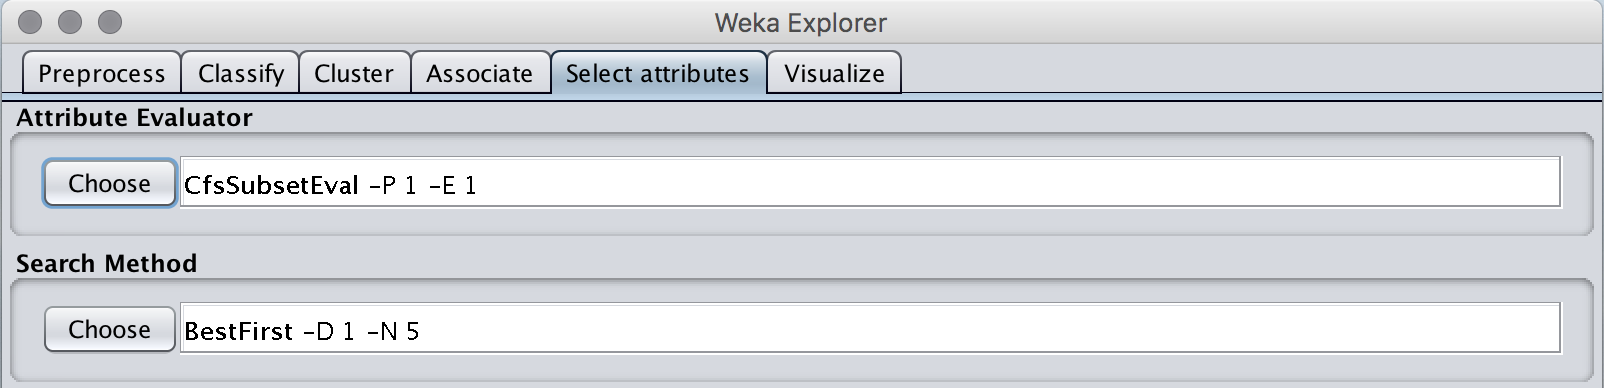
\includegraphics[width=0.9\textwidth]{images/B2_30.png}
\caption{Attribute selection: specifying an evaluator and a search method.}
\label{fig:att_selection_config}
\end{figure}

Figure~\ref{fig:att_selection_config} shows that part of WEKA's
attribute selection panel where you specify the attribute evaluator
and search method. Attribute selection is normally done by searching
the space of attribute subsets, evaluating each one. A potentially
faster but less accurate approach is to evaluate the attributes
individually and sort them, discarding attributes that fall below a
chosen cut-off point.

\subsection{Attribute subset evaluators}

Subset evaluators take a subset of attributes and return a numerical
measure that guides the search. They are configured like any other
WEKA object. \textit{CfsSubsetEval} assesses the predictive ability of
each attribute individually and the degree of redundancy among them,
preferring sets of attributes that are highly correlated with the
class but with low intercorrelation. An option iteratively adds
attributes that have the highest correlation with the class, provided
that the set does not already contain an attribute whose correlation
with the attribute in question is even higher. Missing can be treated
as a separate value, or its counts can be distributed among other
values in proportion to their frequency.

Whereas \textit{CfsSubsetEval} is a filter method of attribute
selection, \textit{WrapperSubsetEval} implements a wrapper
method. \textit{WrapperSubsetEval} uses a classifier to evaluate
attribute set and employs cross-validation to estimate the accuracy of
the learning scheme for each set.

\subsection{Single-attribute evaluators}

Single-attribute evaluators are used with the \textit{Ranker} search
method to generate a ranked list from which \textit{Ranker} discards a
given number (explained in the next
subsection). \textit{ReliefFAttributeEval} is instance-based: it
samples instances randomly and checks neighboring instances of the
same and different classes. It operates on discrete and continuous
class data. Parameters specify the number of instances to sample, the
number of neighbors to check, whether to weight neighbors by distance,
and an exponential function that governs how rapidly weights decay
with distance.

\textit{InfoGainAttributeEval} evaluates attributes by measuring their
information gain with respect to the class. It discretizes numeric
attributes first using the MDL-based discretization method (it can be
set to binarize them instead). This method, along with the next three,
can treat missing as a separate value or distribute the counts among
other values in proportion to their
frequency. \textit{ChiSquaredAttributeEval} evaluates attributes by
computing the chi-squared statistic with respect to the
class. GainRatioAttributeEval evaluates attributes by measuring their
gain ratio with respect to the
class. \textit{SymmetricalUncertAttributeEval} evaluates an attribute
by measuring its symmetrical uncertainty with respect to the class.

\textit{OneRAttributeEval} uses the simple accuracy measure adopted by
the \textit{OneR} classifier. It can use the training data for
evaluation, as OneR does, or it can apply internal cross-validation:
the number of folds is a parameter. It adopts \textit{OneR's} simple
discretization method: the minimum bucket size is a parameter.

Unlike other single-attribute evaluators, \textit{PrincipalComponents}
transforms the set of attributes. The new attributes are ranked in
order of their eigenvalues. Optionally, a subset is selected by
choosing sufficient eigenvectors to account for a given proportion of
the variance (95\% by default). Finally, the reduced data can be
transformed back to the original space.

\subsection{Search methods}

Search methods traverse the attribute space to find a good
subset. Quality is measured by the chosen attribute subset
evaluator. Each search method can be configured with WEKA's object
editor. \textit{BestFirst} performs greedy hill climbing with
backtracking; you can specify how many consecutive nonimproving nodes
must be encountered before the system backtracks. It can search
forward from the empty set of attributes, backward from the full set,
or start at an intermediate point (specified by a list of attribute
indexes) and search in both directions by considering all possible
single-attribute additions and deletions. Subsets that have been
evaluated are cached for efficiency; the cache size is a parameter.

\textit{GreedyStepwise} searches greedily through the space of
attribute subsets. Like \textit{BestFirst}, it may progress forward
from the empty set or backward from the full set. Unlike
\textit{BestFirst}, it does not backtrack but terminates as soon as
adding or deleting the best remaining attribute decreases the
evaluation metric. In an alternative mode, it ranks attributes by
traversing the space from empty to full (or vice versa) and recording
the order in which attributes are selected. You can specify the number
of attributes to retain or set a threshold below which attributes are
discarded.

Finally we describe \textit{Ranker}, which as noted earlier is not a
search method for attribute subsets but a ranking scheme for
individual attributes. It sorts attributes by their individual
evaluations and must be used in conjunction with one of the
single-attribute evaluators---not an attribute subset
evaluator. \textit{Ranker} not only ranks attributes but also performs
attribute selection by removing the lower-ranking ones. You can set a
cut-off threshold below which attributes are discarded, or specify how
many attributes to retain. You can specify certain attributes that
must be retained regardless of their rank.



\chapter{Experimenter}
%
%    This program is free software; you can redistribute it and/or modify
%    it under the terms of the GNU General Public License as published by
%    the Free Software Foundation; either version 2 of the License, or
%    (at your option) any later version.
%
%    This program is distributed in the hope that it will be useful,
%    but WITHOUT ANY WARRANTY; without even the implied warranty of
%    MERCHANTABILITY or FITNESS FOR A PARTICULAR PURPOSE.  See the
%    GNU General Public License for more details.
%
%    You should have received a copy of the GNU General Public License
%    along with this program; if not, write to the Free Software
%    Foundation, Inc., 675 Mass Ave, Cambridge, MA 02139, USA.
%

% Version: $Revision$

%%%%%%%%%%%%%%%%
% Introduction %
%%%%%%%%%%%%%%%%

\section{Introduction}

The Weka Experiment Environment enables the user to create, run, modify, and analyse experiments in a more convenient manner than is possible when processing the schemes individually. For example, the user can create an experiment that runs several schemes against a series of datasets and then analyse the results to determine if one of the schemes is (statistically) better than the other schemes.

The Experiment Environment can be run from the command line using the Simple CLI. For example, the following commands could be typed into the CLI to run the \texttt{OneR} scheme on the Iris dataset using a basic train and test process. (Note that the commands would be typed on one line into the CLI.)

\begin{verbatim}
java weka.experiment.Experiment -r -T data/iris.arff
  -D weka.experiment.InstancesResultListener
  -P weka.experiment.RandomSplitResultProducer --
  -W weka.experiment.ClassifierSplitEvaluator --
  -W weka.classifiers.rules.OneR
\end{verbatim}

While commands can be typed directly into the CLI, this technique is not particularly convenient and the experiments are not easy to modify.

The Experimenter comes in two flavours, either with a simple interface that provides most of the functionality one needs for experiments, or with an interface with full access to the Experimenter's capabilities. You can choose between those two with the \textit{Experiment Configuration Mode} radio buttons:

\begin{itemize}
	\item Simple
	\item Advanced 
\end{itemize}

Both setups allow you to setup \textit{standard} experiments, that are run locally on a single machine, or remote experiments, which are distributed between several hosts. The distribution of experiments cuts down the time the experiments will take until completion, but on the other hand the setup takes more time.

The next section covers the \textit{standard} experiments (both, simple and advanced), followed by the \textit{remote} experiments and finally the \textit{analysing} of the results.


%%%%%%%%%%%%%%%%%%%%%%%%
% Standard Experiments %
%%%%%%%%%%%%%%%%%%%%%%%%

\newpage
\section{Standard Experiments}

%%%%%%%%%%
% Simple %
%%%%%%%%%%

\subsection{Simple}

\subsubsection{New experiment}

After clicking \textit{New} default parameters for an Experiment are defined.

\begin{center}
	\epsfig{file=images/experimenter/simple_new.eps,width=10cm}
\end{center}


\subsubsection{Results destination}

By default, an ARFF file is the destination for the results output. But you can choose between

\begin{itemize}
	\item ARFF file
   \item CSV file
   \item JDBC database 
\end{itemize}

ARFF file and JDBC database are discussed in detail in the following sections. CSV is similar to ARFF, but it can be used to be loaded in an external spreadsheet application.


\subsubsection*{ARFF file}

If the file name is left empty a temporary file will be created in the TEMP directory of the system. If one wants to specify an explicit results file, click on \textit{Browse} and choose a filename, e.g., \textit{Experiment1.arff}.

\begin{center}
	\epsfig{file=images/experimenter/simple_saveoutput_ARFF1.eps,width=7cm}
\end{center}


Click on \textit{Save} and the name will appear in the edit field next to \textit{ARFF file}.

\begin{center}
	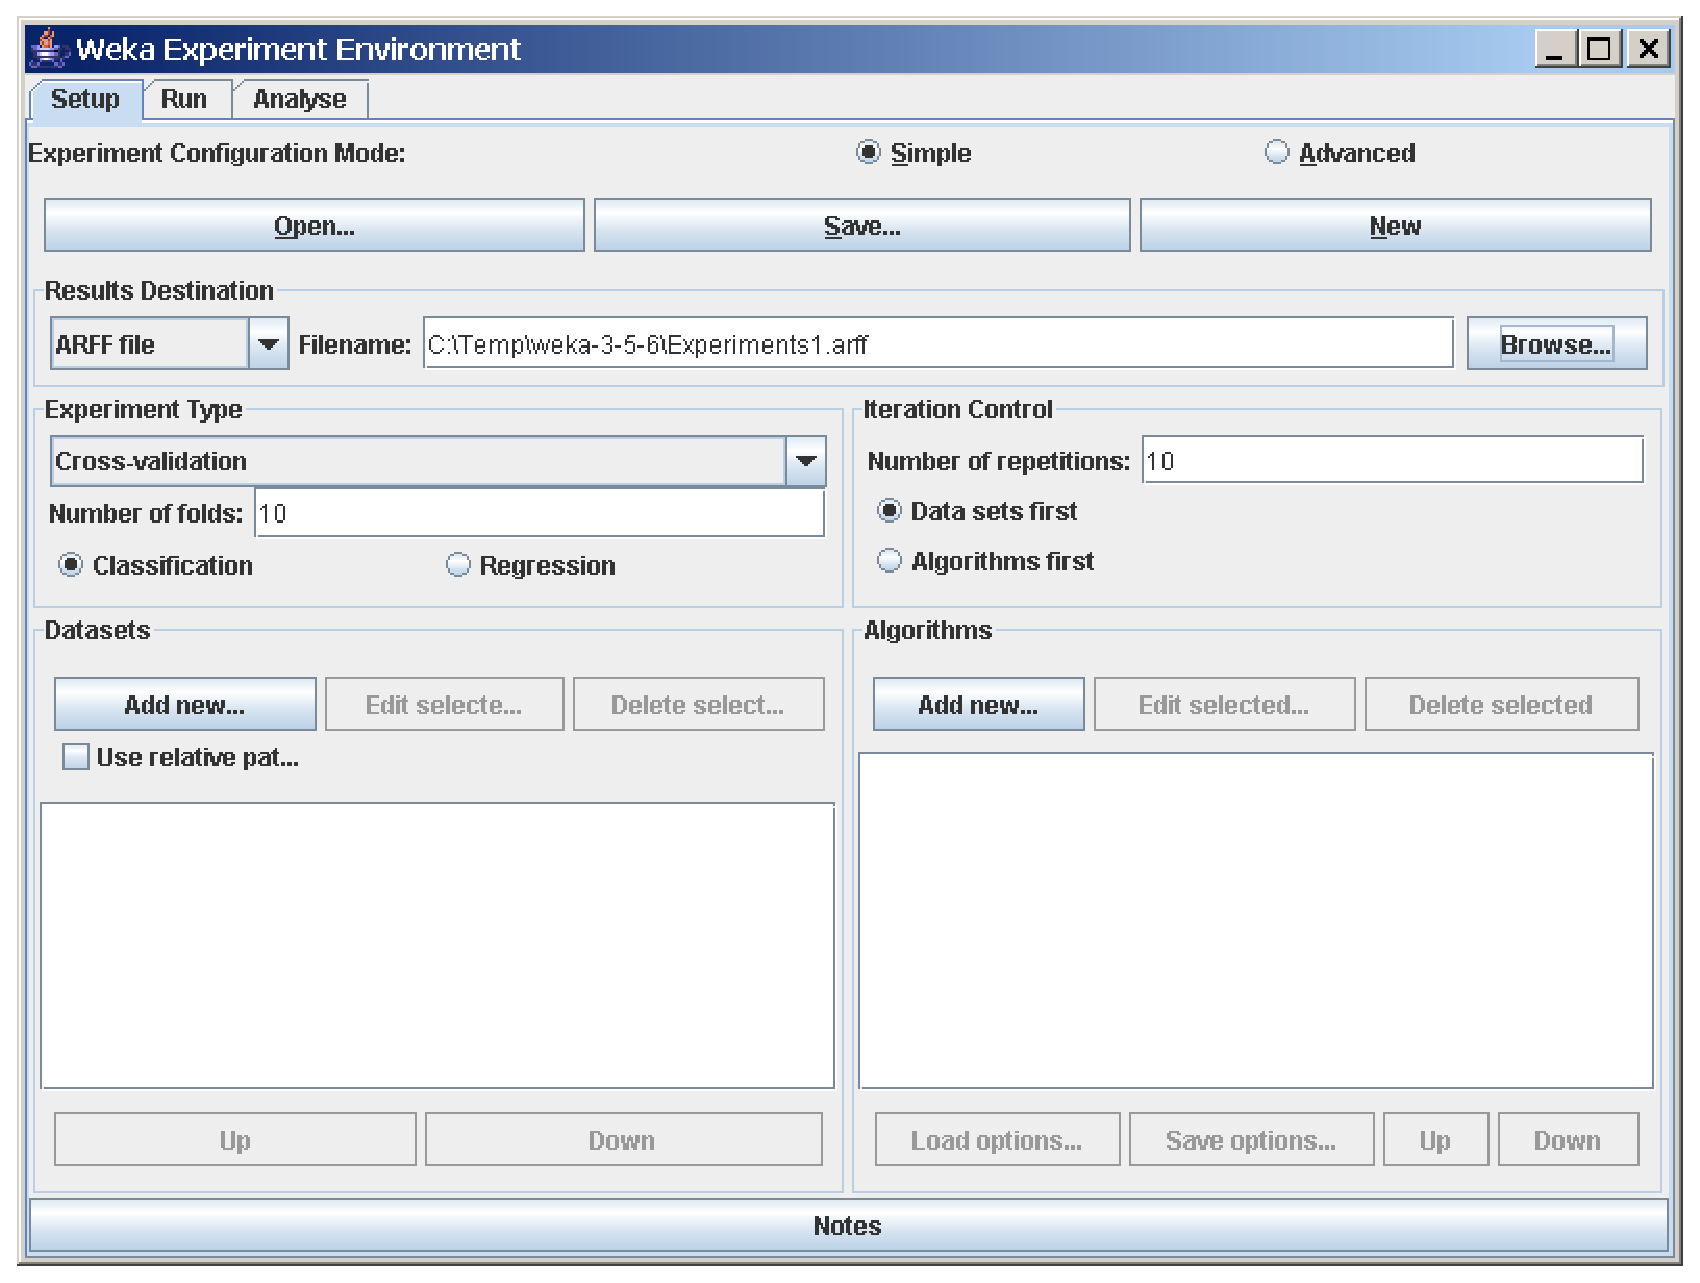
\epsfig{file=images/experimenter/simple_saveoutput_ARFF2.eps,width=10cm}
\end{center}


The advantage of ARFF or CSV files is that they can be created without any additional classes besides the ones from Weka. The drawback is the lack of the ability to resume an experiment that was interrupted, e.g., due to an error or the addition of dataset or algorithms. Especially with time-consuming experiments, this behavior can be annoying.


\subsubsection*{JDBC database}

With JDBC it is easy to store the results in a database. The necessary jar archives have to be in the CLASSPATH to make the JDBC functionality of a particular database available.

After changing \textit{ARFF file} to \textit{JDBC database} click on \textit{User...} to specify JDBC URL and user credentials for accessing the database.

\begin{center}
	\epsfig{file=images/experimenter/simple_saveoutput_JDBC1.eps,width=8cm}
\end{center}


After supplying the necessary data and clicking on \textit{OK}, the URL in the main window will be updated.

\textit{Note:} at this point, the database connection is not tested; this is done when the experiment is started.

\begin{center}
	\epsfig{file=images/experimenter/simple_saveoutput_JDBC2.eps,width=10cm}
\end{center}


The advantage of a JDBC database is the possibility to resume an interrupted or extended experiment. Instead of re-running all the other algorithm/dataset combinations again, only the missing ones are computed.


\subsubsection{Experiment type}

The user can choose between the following three different types

\begin{itemize}
	\item \textbf{Cross-validation (default)} \\
      performs stratified cross-validation with the given number of folds 

   \item \textbf{Train/Test Percentage Split (data randomized)} \\
      splits a dataset according to the given percentage into a train and a test file (one cannot specify explicit training and test files in the Experimenter), after the order of the data has been randomized and stratified
	
	\begin{center}
		\epsfig{file=images/experimenter/simple_experimenttype1.eps,width=10cm}
	\end{center}

    \item \textbf{Train/Test Percentage Split (order preserved)} \\
      because it is impossible to specify an explicit train/test files pair, one can \textit{abuse} this type to \textit{un-merge} previously merged train and test file into the two original files (one only needs to find out the correct percentage) 
	
	\begin{center}
		\epsfig{file=images/experimenter/simple_experimenttype2.eps,width=10cm}
	\end{center}
	
\end{itemize}

Additionally, one can choose between \textit{Classification} and \textit{Regression}, depending on the datasets and classifiers one uses. For decision trees like \texttt{J48} (Weka's implementation of Quinlan's C4.5 \cite{quinlan}) and the iris dataset, \textit{Classification} is necessary, for a numeric classifier like \texttt{M5P}, on the other hand, \textit{Regression}. \textit{Classification} is selected by default.

\textit{Note:} if the percentage splits are used, one has to make sure that the corrected paired \textit{T-Tester} still produces sensible results with the given ratio \cite{bengio}.


\subsubsection{Datasets}

One can add dataset files either with an absolute path or with a relative one. The latter makes it often easier to run experiments on different machines, hence one should check \textit{Use relative paths}, before clicking on \textit{Add new...}.

\begin{center}
	\epsfig{file=images/experimenter/simple_adddataset1.eps,width=7cm}
\end{center}


In this example, open the \textit{data} directory and choose the \textit{iris.arff} dataset.

\begin{center}
	\epsfig{file=images/experimenter/simple_adddataset2.eps,width=7cm}
\end{center}


After clicking \textit{Open} the file will be displayed in the datasets list. If one selects a directory and hits \textit{Open}, then all ARFF files will be added recursively. Files can be deleted from the list by selecting them and then clicking on \textit{Delete selected}.

ARFF files are not the only format one can load, but \textit{all} files that can be converted with Weka's \textit{``core converters''}. The following formats are currently supported:

\begin{itemize}
	\item ARFF (+ compressed)
	\item C4.5
	\item CSV
	\item libsvm
	\item binary serialized instances
	\item XRFF (+ compressed)
\end{itemize}

By default, the class attribute is assumed to be the last attribute. But if a data format contains information about the class attribute, like XRFF or C4.5, this attribute will be used instead.

\begin{center}
	\epsfig{file=images/experimenter/simple_adddataset3.eps,width=10cm}
\end{center}


\subsubsection{Iteration control}

\begin{itemize}
   \item \textbf{Number of repetitions} \\
      In order to get statistically meaningful results, the default number of iterations is 10. In case of 10-fold cross-validation this means 100 calls of one classifier with training data and tested against test data. 

   \item \textbf{Data sets first/Algorithms first} \\
      As soon as one has more than one dataset and algorithm, it can be useful to switch from datasets being iterated over first to algorithms. This is the case if one stores the results in a database and wants to complete the results for all the datasets for one algorithm as early as possible. 
\end{itemize}


\subsubsection{Algorithms}

New algorithms can be added via the \textit{Add new...} button. Opening this dialog for the first time, \texttt{ZeroR} is presented, otherwise the one that was selected last.

\begin{center}
	\epsfig{file=images/experimenter/simple_addalgorithm1.eps,width=6cm}
\end{center}


With the \textit{Choose} button one can open the \textit{GenericObjectEditor} and choose another classifier.

\begin{center}
	\epsfig{file=images/experimenter/simple_addalgorithm2.eps,width=6cm}
\end{center}

The \textit{Filter...} button enables one to highlight classifiers that can handle certain attribute and class types. With the \textit{Remove filter} button all the selected capabilities will get cleared and the highlighting removed again.

Additional algorithms can be added again with the \textit{Add new...} button, e.g., the \texttt{J48} decision tree.

\begin{center}
	\epsfig{file=images/experimenter/simple_addalgorithm3.eps,width=6cm}
\end{center}


After setting the classifier parameters, one clicks on \textit{OK} to add it to the list of algorithms.

\begin{center}
	\epsfig{file=images/experimenter/simple_addalgorithm4.eps,width=10cm}
\end{center}


With the \textit{Load options...} and \textit{Save options...} buttons one can load and save the setup of a selected classifier from and to XML. This is especially useful for highly configured classifiers (e.g., nested meta-classifiers), where the manual setup takes quite some time, and which are used often.

One can also paste classifier settings here by right-clicking (or \textit{Alt-Shift-left-clicking}) and selecting the appropriate menu point from the popup menu, to either add a new classifier or replace the selected one with a new setup. This is rather useful for transferring a classifier setup from the Weka Explorer over to the Experimenter without having to setup the classifier from scratch.

\subsubsection{Saving the setup}

For future re-use, one can save the current setup of the experiment to a file by clicking on \textit{Save...} at the top of the window.

\begin{center}
	\epsfig{file=images/experimenter/simple_save.eps,width=7cm}
\end{center}


By default, the format of the experiment files is the binary format that Java serialization offers. The drawback of this format is the possible incompatibility between different versions of Weka. A more robust alternative to the binary format is the XML format.

Previously saved experiments can be loaded again via the \textit{Open...} button.


\subsubsection{Running an Experiment}

To run the current experiment, click the \textit{Run} tab at the top of the Experiment Environment window. The current experiment performs 10 runs of 10-fold stratified cross-validation on the Iris dataset using the \texttt{ZeroR} and \texttt{J48} scheme.

\begin{center}
	\epsfig{file=images/experimenter/runexperiment1.eps,width=10cm}
\end{center}


Click \textit{Start} to run the experiment.

\begin{center}
	\epsfig{file=images/experimenter/runexperiment2.eps,width=10cm}
\end{center}


If the experiment was defined correctly, the 3 messages shown above will be displayed in the \textit{Log} panel. The results of the experiment are saved to the dataset \textit{Experiment1.arff}. 

%%%%%%%%%%%%
% Advanced %
%%%%%%%%%%%%

\newpage
\subsection{Advanced}

\subsubsection{Defining an Experiment}

When the Experimenter is started in \textit{Advanced} mode, the \textit{Setup} tab is displayed. Click \textit{New} to initialize an experiment. This causes default parameters to be defined for the experiment.
\begin{center}
	\epsfig{file=images/experimenter/advanced_new.eps,width=10cm}
\end{center}

To define the dataset to be processed by a scheme, first select \textit{Use relative paths} in the \textit{Datasets} panel of the \textit{Setup} tab and then click on \textit{Add new...} to open a dialog window.
\begin{center}
	\epsfig{file=images/experimenter/advanced_adddataset1.eps,width=7cm}
\end{center}

Double click on the \textit{data} folder to view the available datasets or navigate to an alternate location. Select \textit{iris.arff} and click \textit{Open} to select the Iris dataset.
\begin{center}
	\epsfig{file=images/experimenter/advanced_adddataset2.eps,width=7cm}
\end{center}
	
\begin{center}
	\epsfig{file=images/experimenter/advanced_adddataset3.eps,width=10cm}
\end{center}

The dataset name is now displayed in the \textit{Datasets} panel of the \textit{Setup} tab.



\subsubsection*{Saving the Results of the Experiment}

To identify a dataset to which the results are to be sent, click on the \textit{InstancesResultListener} entry in the \textit{Destination} panel. The output file parameter is near the bottom of the window, beside the text \textit{outputFile}. Click on this parameter to display a file selection window.
\begin{center}
	\epsfig{file=images/experimenter/advanced_saveoutput1.eps,width=6cm}
\end{center}
	
\begin{center}
	\epsfig{file=images/experimenter/advanced_saveoutput2.eps,width=7cm}
\end{center}

Type the name of the output file and click \textit{Select}. The file name is displayed in the \textit{outputFile} panel. Click on \textit{OK} to close the window.
\begin{center}
	\epsfig{file=images/experimenter/advanced_saveoutput3.eps,width=6cm}
\end{center}

The dataset name is displayed in the \textit{Destination} panel of the \textit{Setup} tab.
\begin{center}
	\epsfig{file=images/experimenter/advanced_saveoutput4.eps,width=10cm}
\end{center}



\subsubsection*{Saving the Experiment Definition}

The experiment definition can be saved at any time. Select \textit{Save...} at the top of the \textit{Setup} tab. Type the dataset name with the extension \textit{exp} (or select the dataset name if the experiment definition dataset already exists) for binary files or choose \textit{Experiment configuration files (*.xml)} from the file types combobox (the XML files are robust with respect to version changes).
\begin{center}
	\epsfig{file=images/experimenter/advanced_save.eps,width=7cm}
\end{center}


The experiment can be restored by selecting \textit{Open} in the \textit{Setup} tab and then selecting \textit{Experiment1.exp} in the dialog window.



\subsubsection{Running an Experiment}

To run the current experiment, click the \textit{Run} tab at the top of the Experiment Environment window. The current experiment performs 10 randomized train and test runs on the Iris dataset, using 66\% of the patterns for training and 34\% for testing, and using the \texttt{ZeroR} scheme.
\begin{center}
	\epsfig{file=images/experimenter/runexperiment1.eps,width=10cm}
\end{center}

Click \textit{Start} to run the experiment.
\begin{center}
	\epsfig{file=images/experimenter/runexperiment2.eps,width=10cm}
\end{center}

If the experiment was defined correctly, the 3 messages shown above will be displayed in the \textit{Log} panel. The results of the experiment are saved to the dataset \textit{Experiment1.arff}. The first few lines in this dataset are shown below.

\begin{verbatim}
 @relation InstanceResultListener
 
 @attribute Key_Dataset {iris}
 @attribute Key_Run {1,2,3,4,5,6,7,8,9,10}
 @attribute Key_Scheme {weka.classifiers.rules.ZeroR,weka.classifiers.trees.J48}
 @attribute Key_Scheme_options {,'-C 0.25 -M 2'}
 @attribute Key_Scheme_version_ID {48055541465867954,-217733168393644444}
 @attribute Date_time numeric
 @attribute Number_of_training_instances numeric
 @attribute Number_of_testing_instances numeric
 @attribute Number_correct numeric
 @attribute Number_incorrect numeric
 @attribute Number_unclassified numeric
 @attribute Percent_correct numeric
 @attribute Percent_incorrect numeric
 @attribute Percent_unclassified numeric
 @attribute Kappa_statistic numeric
 @attribute Mean_absolute_error numeric
 @attribute Root_mean_squared_error numeric
 @attribute Relative_absolute_error numeric
 @attribute Root_relative_squared_error numeric
 @attribute SF_prior_entropy numeric
 @attribute SF_scheme_entropy numeric
 @attribute SF_entropy_gain numeric
 @attribute SF_mean_prior_entropy numeric
 @attribute SF_mean_scheme_entropy numeric
 @attribute SF_mean_entropy_gain numeric
 @attribute KB_information numeric
 @attribute KB_mean_information numeric
 @attribute KB_relative_information numeric
 @attribute True_positive_rate numeric
 @attribute Num_true_positives numeric
 @attribute False_positive_rate numeric
 @attribute Num_false_positives numeric
 @attribute True_negative_rate numeric
 @attribute Num_true_negatives numeric
 @attribute False_negative_rate numeric
 @attribute Num_false_negatives numeric
 @attribute IR_precision numeric
 @attribute IR_recall numeric
 @attribute F_measure numeric
 @attribute Area_under_ROC numeric
 @attribute Time_training numeric
 @attribute Time_testing numeric
 @attribute Summary {'Number of leaves: 3\nSize of the tree: 5\n',
    'Number of leaves: 5\nSize of the tree: 9\n',
    'Number of leaves: 4\nSize of the tree: 7\n'}
 @attribute measureTreeSize numeric
 @attribute measureNumLeaves numeric
 @attribute measureNumRules numeric

 @data
 
 iris,1,weka.classifiers.rules.ZeroR,,48055541465867954,20051221.033,99,51,
 17,34,0,33.333333,66.666667,0,0,0.444444,0.471405,100,100,80.833088,80.833088,
 0,1.584963,1.584963,0,0,0,0,1,17,1,34,0,0,0,0,0.333333,1,0.5,0.5,0,0,?,?,?,?
\end{verbatim}




\subsubsection{Changing the Experiment Parameters}

\subsubsection*{Changing the Classifier}

The parameters of an experiment can be changed by clicking on the \textit{Result generator} panel.
\begin{center}
	\epsfig{file=images/experimenter/advanced_changeparameters1.eps,width=6cm}
\end{center}

The \textit{RandomSplitResultProducer} performs repeated train/test runs. The number of instances (expressed as a percentage) used for training is given in the \textit{trainPercent} box. (The number of runs is specified in the \textit{Runs} panel in the \textit{Setup} tab.)

A small help file can be displayed by clicking \textit{More} in the \textit{About} panel.
\begin{center}
	\epsfig{file=images/experimenter/advanced_changeparameters2.eps,width=6cm}
\end{center}

Click on the \textit{splitEvaluator} entry to display the \textit{SplitEvaluator} properties.
\begin{center}
	\epsfig{file=images/experimenter/advanced_changeparameters3.eps,width=6cm}
\end{center}

Click on the classifier entry (\texttt{ZeroR}) to display the scheme properties.
\begin{center}
	\epsfig{file=images/experimenter/advanced_changeparameters4.eps,width=6cm}
\end{center}

This scheme has no modifiable properties (besides \textit{debug} mode on/off) but most other schemes do have properties that can be modified by the user. The \textit{Capabilities} button opens a small dialog listing all the attribute and class types this classifier can handle. Click on the \textit{Choose} button to select a different scheme. The window below shows the parameters available for the \texttt{J48} decision-tree scheme. If desired, modify the parameters and then click \textit{OK} to close the window.
\begin{center}
	\epsfig{file=images/experimenter/advanced_changeparameters5.eps,width=6cm}
\end{center}

The name of the new scheme is displayed in the \textit{Result generator} panel.
\begin{center}
	\epsfig{file=images/experimenter/advanced_changeparameters6.eps,width=10cm}
\end{center}


\subsubsection*{Adding Additional Schemes}

Additional schemes can be added in the \textit{Generator properties} panel. To begin, change the drop-down list entry from \textit{Disabled} to \textit{Enabled} in the \textit{Generator properties} panel.
\begin{center}
	\epsfig{file=images/experimenter/advanced_additionalschemes1.eps,width=10cm}
\end{center}

Click \textit{Select property} and expand \textit{splitEvaluator} so that the \textit{classifier} entry is visible in the property list; click \textit{Select}.
\begin{center}
	\epsfig{file=images/experimenter/advanced_additionalschemes2.eps,width=3.5cm}
\end{center}

The scheme name is displayed in the \textit{Generator properties} panel.
\begin{center}
	\epsfig{file=images/experimenter/advanced_additionalschemes3.eps,width=10cm}
\end{center}

To add another scheme, click on the \textit{Choose} button to display the \textit{GenericObjectEditor} window.
\begin{center}
	\epsfig{file=images/experimenter/advanced_additionalschemes4.eps,width=10cm}
\end{center}

The \textit{Filter...} button enables one to highlight classifiers that can handle certain attribute and class types. With the \textit{Remove filter} button all the selected capabilities will get cleared and the highlighting removed again.

To change to a decision-tree scheme, select \texttt{J48} (in subgroup \textit{trees}).
\begin{center}
	\epsfig{file=images/experimenter/advanced_additionalschemes5.eps,width=6cm}
\end{center}

The new scheme is added to the \textit{Generator properties} panel. Click \textit{Add} to add the new scheme.
\begin{center}
	\epsfig{file=images/experimenter/advanced_additionalschemes6.eps,width=10cm}
\end{center}

Now when the experiment is run, results are generated for both schemes.

To add additional schemes, repeat this process. To remove a scheme, select the scheme by clicking on it and then click \textit{Delete}.


\subsubsection*{Adding Additional Datasets}

The scheme(s) may be run on any number of datasets at a time. Additional datasets are added by clicking \textit{Add new...} in the \textit{Datasets} panel. Datasets are deleted from the experiment by selecting the dataset and then clicking \textit{Delete Selected}.


\subsubsection*{Raw Output}

The raw output generated by a scheme during an experiment can be saved to a file and then examined at a later time. Open the \textit{ResultProducer} window by clicking on the \textit{Result generator} panel in the \textit{Setup} tab.
\begin{center}
	\epsfig{file=images/experimenter/advanced_rawoutput1.eps,width=6cm}
\end{center}

Click on \textit{rawOutput} and select the \textit{True} entry from the drop-down list. By default, the output is sent to the zip file \textit{splitEvaluatorOut.zip}. The output file can be changed by clicking on the \textit{outputFile} panel in the window. Now when the experiment is run, the result of each processing run is archived, as shown below.
\begin{center}
	\epsfig{file=images/experimenter/advanced_rawoutput2.eps,width=10cm}
\end{center}

The contents of the first run are:

\begin{verbatim}
ClassifierSplitEvaluator: weka.classifiers.trees.J48 -C 0.25 -M 2(version 
     -217733168393644444)Classifier model: 
J48 pruned tree
------------------

petalwidth <= 0.6: Iris-setosa (33.0)
petalwidth > 0.6
|   petalwidth <= 1.5: Iris-versicolor (31.0/1.0)
|   petalwidth > 1.5: Iris-virginica (35.0/3.0) 

Number of Leaves  : 	3

Size of the tree : 	5 


Correctly Classified Instances          47               92.1569 %
Incorrectly Classified Instances         4                7.8431 %
Kappa statistic                          0.8824
Mean absolute error                      0.0723
Root mean squared error                  0.2191
Relative absolute error                 16.2754 %
Root relative squared error             46.4676 %
Total Number of Instances               51     
measureTreeSize : 5.0
measureNumLeaves : 3.0
measureNumRules : 3.0
\end{verbatim}



\subsubsection{Other Result Producers}

\subsubsection*{Cross-Validation Result Producer}

To change from random train and test experiments to cross-validation experiments, click on the \textit{Result generator} entry. At the top of the window, click on the drop-down list and select \textit{CrossValidationResultProducer}. The window now contains parameters specific to cross-validation such as the number of partitions/folds. The experiment performs 10-fold cross-validation instead of train and test in the given example.
\begin{center}
	\epsfig{file=images/experimenter/advanced_cvresultproducer1.eps,width=6cm}
\end{center}

The \textit{Result generator} panel now indicates that cross-validation will be performed. Click on \textit{More} to generate a brief description of the \textit{CrossValidationResultProducer}.
\begin{center}
	\epsfig{file=images/experimenter/advanced_cvresultproducer2.eps,width=6cm}
\end{center}

As with the \textit{RandomSplitResultProducer}, multiple schemes can be run during cross-validation by adding them to the \textit{Generator properties} panel.
\begin{center}
	\epsfig{file=images/experimenter/advanced_cvresultproducer3.eps,width=10cm}
\end{center}

The number of runs is set to 1 in the \textit{Setup} tab in this example, so that only one run of cross-validation for each scheme and dataset is executed.

When this experiment is analysed, the following results are generated. Note that there are 30 (1 run times 10 folds times 3 schemes) result lines processed.
\begin{center}
	\epsfig{file=images/experimenter/advanced_cvresultproducer4.eps,width=10cm}
\end{center}


\subsubsection*{Averaging Result Producer}

An alternative to the \textit{CrossValidationResultProducer} is the \textit{AveragingResultProducer}. This result producer takes the average of a set of runs (which are typically cross-validation runs). This result producer is identified by clicking the \textit{Result generator} panel and then choosing the \textit{AveragingResultProducer} from the \textit{GenericObjectEditor}.
\begin{center}
	\epsfig{file=images/experimenter/advanced_averagingresultproducer1.eps,width=6cm}
\end{center}

The associated help file is shown below.
\begin{center}
	\epsfig{file=images/experimenter/advanced_averagingresultproducer2.eps,width=6cm}
\end{center}

Clicking the \textit{resultProducer} panel brings up the following window.
\begin{center}
	\epsfig{file=images/experimenter/advanced_averagingresultproducer3.eps,width=6cm}
\end{center}

As with the other ResultProducers, additional schemes can be defined. When the \textit{AveragingResultProducer} is used, the classifier property is located deeper in the \textit{Generator properties} hierarchy.
\begin{center}
	\epsfig{file=images/experimenter/advanced_averagingresultproducer4.eps,width=3.5cm}
\end{center}
	
\begin{center}
	\epsfig{file=images/experimenter/advanced_averagingresultproducer5.eps,width=10cm}
\end{center}

In this experiment, the \texttt{ZeroR}, \texttt{OneR}, and \texttt{J48} schemes are run 10 times with 10-fold cross-validation. Each set of 10 cross-validation folds is then averaged, producing one result line for each run (instead of one result line for each fold as in the previous example using the \textit{CrossValidationResultProducer}) for a total of 30 result lines. If the raw output is saved, all 300 results are sent to the archive.
\begin{center}
	\epsfig{file=images/experimenter/advanced_averagingresultproducer6.eps,width=10cm}
\end{center}


\subsubsection*{Explicit Test-Set Result Producer}

One of the Experimenter's biggest drawbacks in the past was the inability to supply test sets. Even though repeated runs with explicit test sets don't make that much sense (apart from randomizing the training data, to test the robustness of the classifier), it offers the possibility to compare different classifiers and classifier setups side-by-side; a feature that the Explorer lacks.

This result producer can be used by clicking the \textit{Result generator} panel and then choosing the \textit{ExplicitTestSetResultProducer} from the \textit{GenericObjectEditor}.
\begin{center}
	\epsfig{file=images/experimenter/advanced_explicittestsetresultproducer1.eps,width=6cm}
\end{center}

The associated help file is shown below.
\begin{center}
	\epsfig{file=images/experimenter/advanced_explicittestsetresultproducer2.eps,width=10cm}
\end{center}

The experiment setup using explicit test sets requires a bit more care than the others. The reason for this is, that the result producer has no information about the file the data originates from. In order to identify the correct test set, this result producer utilizes the relation name of the training file. Here is how the file name gets constructed under a Unix-based operating system (Linux, Mac OSX), based on the result producer's setup and the current training set's relation name:
\begin{verbatim}
   testsetDir "/" testsetPrefix + relation-name + testsetSuffix
\end{verbatim}

\noindent With the \texttt{testsetDir} property set to \texttt{/home/johndoe/datasets/test}, an empty \texttt{testsetPrefix}, \texttt{anneal} as \texttt{relation-name} and the default \texttt{testsetSuffix}, i.e., \texttt{\_test.arff}, the following file name for the test set gets created:
\begin{verbatim}
   /home/johndoe/datasets/test/anneal_test.arff
\end{verbatim}

\noindent \textbf{NB:} The result producer is platform-aware and uses backslashes instead of forward slashes on MS Windows-based operating systems.

Of course, the relation name might not always be as simple as in the above example. Especially not, when the dataset has been pre-processed with various filters before being used in the Experimenter. The \textit{ExplicitTestSetResultProducer} allows one to remove unwanted strings from relation name using regular expressions. In case of removing the WEKA filter setups that got appended to the relation name during pre-processing, one can simply use \texttt{-weka.*} as the value for \texttt{relationFind} and leave \texttt{relationReplace} empty.

Using this setup, the following relation name:
\begin{verbatim}
   anneal-weka.filters.unsupervised.instance.RemovePercentage-P66.0
\end{verbatim}
\noindent will be turned into this:
\begin{verbatim}
   anneal
\end{verbatim}

As long as one takes care and uses sensible relation names, the \textit{ExplicitTestSetResultProducer} can be used to compare different classifiers and setups on train/test set pairs, using the full functionality of the Experimenter.

%%%%%%%%%%%%%%%%%%%%%%%
% Cluster experiments %
%%%%%%%%%%%%%%%%%%%%%%%

\newpage
\section{Cluster Experiments}
Using the advanced mode of the Experimenter you can now run experiments on
clustering algorithms as well as classifiers (Note: this is a new feature
available with Weka 3.5.8). The main evaluation metric for this type of
experiment is the log likelihood of the clusters found by each clusterer. Here
is an example of setting up a cross-validation experiment using clusterers. \\

\noindent Choose \textit{CrossValidationResultProducer} from the Result generator panel.
\begin{center}
	\epsfig{file=images/experimenter/advanced-clusterexperiments-crossvalidationresultproducer.eps, width=10cm, angle=-90}
\end{center}

\newpage

\noindent Next, choose \textit{DensityBasedClustererSplitEvaluator} as the split evaluator
to use.
\begin{center}
	\epsfig{file=images/experimenter/advanced-clusterexperiments-densitybasedclusterersplitevaluator.eps, width=5cm, angle=-90}
\end{center}

\noindent If you click on \textit{DensityBasedClustererSplitEvaluator} you will see its
options. \\

\noindent \textbf{Note} that there is an option for removing the class column
from the data. In the Experimenter, the class column is set to be the last
column by default. Turn this off if you want to keep this column in the data.
\begin{center}
	\epsfig{file=images/experimenter/advanced-clusterexperiments-densitybasedclusterersplitevaluator2.eps, width=4cm, angle=-90}
\end{center}

\noindent Once \textit{DensityBasedClustererSplitEvaluator} has been selected, you will
notice that the \textit{Generator properties} have become disabled. Enable them
again and expand \textit{splitEvaluator}. Select the \textit{clusterer} node.
\begin{center}
	\epsfig{file=images/experimenter/advanced-clusterexperiments-selectclusterer.eps, width=4cm, angle=-90}
\end{center}

\noindent Now you will see that \textit{EM} becomes the default clusterer and gets added
to the list of schemes. You can now add/delete other clusterers.

\noindent \textbf{IMPORTANT:} in order to
any clusterer that does not produce density estimates (i.e. most other
clusterers in Weka), they will have to wrapped in the
\textit{MakeDensityBasedClusterer}.
\begin{center}
	\epsfig{file=images/experimenter/advanced-clusterexperiments-clustererlist.eps, width=4cm, angle=-90}
\end{center}

\noindent Once and experiment has been run, you can analyze results in the
\textit{Analyse} panel. In the \textit{Comparison} field you will need to scroll
down and select "Log\_likelihood".
\begin{center}
	\epsfig{file=images/experimenter/advanced-clusterexperiments-analyseclusteringexp.eps, width=10cm, angle=-90}
\end{center}

%%%%%%%%%%%%%%%%%%%%%%
% Remote Experiments %
%%%%%%%%%%%%%%%%%%%%%%

\newpage
\section{Remote Experiments}

Remote experiments enable you to distribute the computing load across multiple computers. In the following we will discuss the setup and operation for HSQLDB \cite{hsql} and MySQL \cite{mysql}.

\subsection{Preparation}

To run a remote experiment you will need:

\begin{itemize}
   \item A database server.
   \item A number of computers to run remote engines on.
   \item To edit the remote engine policy file included in the Weka distribution to allow Java class and dataset loading from your home directory.
   \item An invocation of the Experimenter on a machine somewhere (any will do).
\end{itemize}

\noindent For the following examples, we assume a user called \textit{johndoe} with this setup:

\begin{itemize}
	\item Access to a set of computers running a flavour of Unix (pathnames need to be changed for Windows).
   \item The home directory is located at \texttt{/home/johndoe}.
   \item Weka is found in \texttt{/home/johndoe/weka}.
   \item Additional jar archives, i.e., JDBC drivers, are stored in \texttt{/home/johndoe/jars}.
   \item The directory for the datasets is \texttt{/home/johndoe/datasets}.
\end{itemize}

\noindent \textbf{Note:} The example policy file \texttt{remote.policy.example} is using this setup (available in \texttt{weka/experiment}\footnote{Weka's source code can be found in the \texttt{weka-src.jar} archive or obtained from Subversion \cite{subversion}.}).

\subsection{Database Server Setup}

\begin{itemize}
	\item HSQLDB
	
		\begin{itemize}
			\item Download the JDBC driver for HSQLDB, extract the \texttt{hsqldb.jar} and place it in the directory \texttt{/home/johndoe/jars}.
			
			\item To set up the database server, choose or create a directory to run the database server from, and start the server with:

				\begin{verbatim}
java -classpath /home/johndoe/jars/hsqldb.jar \
  org.hsqldb.Server \
  -database.0 experiment -dbname.0 experiment
				\end{verbatim}
				
				\textbf{Note:} This will start up a database with the alias ``experiment'' (\texttt{-dbname.0 <alias>}) and create a properties and a log file at the current location prefixed with ``experiment'' (\texttt{-database.0 <file>}).
				
		\end{itemize}
		
	\item MySQL
	
We won't go into the details of setting up a MySQL server, but this is rather straightforward and includes the following steps:

		\begin{itemize}
  			\item Download a suitable version of MySQL for your server machine.
  			\item Install and start the MySQL server.
  			\item Create a database - for our example we will use \texttt{experiment} as database name.
  			\item Download the appropriate JDBC driver, extract the JDBC jar and place it as \texttt{mysql.jar} in \texttt{/home/johndoe/jars}.
		\end{itemize}
		
\end{itemize}

\subsection{Remote Engine Setup}

\begin{itemize}
   \item First, set up a directory for scripts and policy files: 
		\begin{verbatim}
/home/johndoe/remote_engine
		\end{verbatim}

   \item Unzip the \texttt{remoteExperimentServer.jar} (from the Weka distribution; or build it from the sources\footnote{Weka's source code can be found in the \texttt{weka-src.jar} archive or obtained from Subversion \cite{subversion}.} with \texttt{ant remotejar}) into a temporary directory.

   \item Next, copy \texttt{remoteEngine.jar} and \texttt{remote.policy.example} to the \\ \texttt{/home/johndoe/remote\_engine} directory.

   \item Create a script, called \texttt{/home/johndoe/remote\_engine/startRemoteEngine}, with the following content (don't forget to make it executable with \texttt{chmod a+x startRemoteEngine} when you are on Linux/Unix): 
      \begin{itemize}
      	\item HSQLDB
				\begin{verbatim}
java -Xmx256m \
  -classpath /home/johndoe/jars/hsqldb.jar:remoteEngine.jar:/home/johndoe/weka/weka.jar \
  -Djava.security.policy=remote.policy \
  weka.experiment.RemoteEngine &
				\end{verbatim}
			
			\item MySQL
				\begin{verbatim}
java -Xmx256m \
  -classpath /home/johndoe/jars/mysql.jar:remoteEngine.jar:/home/johndoe/weka/weka.jar \
  -Djava.security.policy=remote.policy \
  weka.experiment.RemoteEngine &
				\end{verbatim}
		\end{itemize}

   \item Now we will start the remote engines that run the experiments on the remote computers (note that the same version of Java must be used for the Experimenter and remote engines):
   	\begin{itemize}
         \item Rename the \texttt{remote.policy.example} file to \texttt{remote.policy}.

         \item For each machine you want to run a remote engine on:
         	\begin{itemize}
         		\item \texttt{ssh} to the machine.
               \item \texttt{cd} to \texttt{/home/johndoe/remote\_engine}.
               \item Run \texttt{/home/johndoe/startRemoteEngine} (to enable the remote engines to use more memory, modify the \texttt{-Xmx} option in the \texttt{startRemoteEngine} script) .
            \end{itemize}
      \end{itemize}
\end{itemize}


\subsection{Configuring the Experimenter}

Now we will run the Experimenter:

\begin{itemize}
	\item HSQLDB
		\begin{itemize}
   		\item Copy the \textit{DatabaseUtils.props.hsql} file from \texttt{weka/experiment} in the \texttt{weka.jar} archive to the \texttt{/home/johndoe/remote\_engine} directory and rename it to \textit{DatabaseUtils.props}.
		   \item Edit this file and change the "\small{\texttt{jdbcURL=jdbc:hsqldb:hsql://server\_name/database\_name}}" entry to include the name of the machine that is running your database server (e.g., \small{\texttt{jdbcURL=jdbc:hsqldb:hsql://dodo.company.com/experiment}}).
		   \item Now start the Experimenter (inside this directory): 
				\small{\begin{verbatim}
java \
  -cp /home/johndoe/jars/hsqldb.jar:remoteEngine.jar:/home/johndoe/weka/weka.jar \
  -Djava.rmi.server.codebase=file:/home/johndoe/weka/weka.jar \
  weka.gui.experiment.Experimenter
				\end{verbatim}}
		\end{itemize}

	\item MySQL
		\begin{itemize}
   		\item Copy the \textit{DatabaseUtils.props.mysql} file from \texttt{weka/experiment} in the \texttt{weka.jar} archive to the \texttt{/home/johndoe/remote\_engine} directory and rename it to \textit{DatabaseUtils.props}.
		   \item Edit this file and change the "\small{\texttt{jdbcURL=jdbc:mysql://server\_name:3306/database\_name}}" entry to include the name of the machine that is running your database server and the name of the database the result will be stored in (e.g., \small{\texttt{jdbcURL=jdbc:mysql://dodo.company.com:3306/experiment}}). 
		   \item Now start the Experimenter (inside this directory): 
				\small{\begin{verbatim}
java \
  -cp /home/johndoe/jars/mysql.jar:remoteEngine.jar:/home/johndoe/weka/weka.jar \
  -Djava.rmi.server.codebase=file:/home/johndoe/weka/weka.jar \
  weka.gui.experiment.Experimenter
				\end{verbatim}}
		\end{itemize}
		
		\textbf{Note:} the database name \textit{experiment} can still be modified in the Experimenter, this is just the default setup.
\end{itemize}

Now we will configure the experiment:

\begin{itemize}
   \item First of all select the \textit{Advanced} mode in the \textit{Setup} tab
   \item Now choose the \textit{DatabaseResultListener} in the \textit{Destination} panel. Configure this result producer:
   	\begin{itemize}
    		\item HSQLDB \\ Supply the value \textbf{sa} for the username and leave the password empty.
    		\item MySQL \\ Provide the username and password that you need for connecting to the database.
    	\end{itemize}
   \item From the \textit{Result generator} panel choose either the \textit{CrossValidationResultProducer} or the \textit{RandomSplitResultProducer} (these are the most commonly used ones) and then configure the remaining experiment details (e.g., datasets and classifiers).
   \item Now enable the \textit{Distribute Experiment} panel by checking the tick box.
   \item Click on the \textit{Hosts} button and enter the names of the machines that you started remote engines on (\texttt{<Enter>} adds the host to the list).
   \item You can choose to distribute by run or dataset.
   \item Save your experiment configuration.
   \item Now start your experiment as you would do normally.
   \item Check your results in the \textit{Analyse} tab by clicking either the \textit{Database} or \textit{Experiment} buttons.
\end{itemize}


\subsection{Multi-core support}
If you want to utilize all the cores on a multi-core machine, then you can do so with Weka version later than 3.5.7. All you have to do, is define the port alongside the hostname in the Experimenter (format: \texttt{hostname:port}) and then start the RemoteEngine with the \texttt{-p} option, specifying the port to listen on.


\subsection{Troubleshooting}

\begin{itemize}
   \item If you get an error at the start of an experiment that looks a bit like this: 

    \texttt{01:13:19: RemoteExperiment (//blabla.company.com/RemoteEngine) (sub)experiment (datataset vineyard.arff) failed : \\ java.sql.SQLException: Table already exists: EXPERIMENT\_INDEX in statement [CREATE TABLE Experiment\_index ( Experiment\_type \\ LONGVARCHAR, Experiment\_setup LONGVARCHAR, Result\_table INT )]} 

    \texttt{01:13:19: dataset :vineyard.arff RemoteExperiment \\ (//blabla.company.com/RemoteEngine) (sub)experiment (datataset vineyard.arff) failed : java.sql.SQLException: Table already exists: EXPERIMENT\_INDEX in statement [CREATE TABLE \\ Experiment\_index ( Experiment\_type LONGVARCHAR, Experiment\_setup LONGVARCHAR, Result\_table INT )]. Scheduling for execution on \\ another host.} 

    then do not panic - this happens because multiple remote machines are trying to create the same table and are temporarily locked out - this will resolve itself so just leave your experiment running - in fact, it is a sign that the experiment is working! 

   \item If you serialized an experiment and then modify your \textit{DatabaseUtils.props} file due to an error (e.g., a missing type-mapping), the Experimenter will use the \textit{DatabaseUtils.props} you had \textit{at the time you serialized the experiment}. Keep in mind that the serialization process also serializes the \textit{DatabaseUtils} class and therefore stored your props-file! This is another reason for storing your experiments as XML and not in the properietary binary format the Java serialization produces. 

   \item Using a corrupt or incomplete \textit{DatabaseUtils.props} file can cause peculiar interface errors, for example disabling the use of the ''User'' button alongside the database URL. If in doubt copy a clean \textit{DatabaseUtils.props} from Subversion \cite{subversion}. 

   \item If you get \texttt{NullPointerException at java.util.Hashtable.get()} in the Remote Engine do not be alarmed. This will have no effect on the results of your experiment. 
\end{itemize}
    
%%%%%%%%%%%%%%%%%%%%%%%%%
% Analysing Experiments %
%%%%%%%%%%%%%%%%%%%%%%%%%

\newpage
\section{Analysing Results}

\subsection{Setup}

Weka includes an experiment analyser that can be used to analyse the results of experiments (in this example, the results were sent to an \textit{InstancesResultListener}). The experiment shown below uses 3 schemes, \texttt{ZeroR}, \texttt{OneR}, and \texttt{J48}, to classify the Iris data in an experiment using 10 train and test runs, with 66\% of the data used for training and 34\% used for testing.
\begin{center}
	\epsfig{file=images/experimenter/analyser01.eps,width=10cm}
\end{center}

After the experiment setup is complete, run the experiment. Then, to analyse the results, select the \textit{Analyse} tab at the top of the Experiment Environment window.

Click on \textit{Experiment} to analyse the results of the current experiment.
\begin{center}
	\epsfig{file=images/experimenter/analyser02.eps,width=10cm}
\end{center}

The number of result lines available (\textit{Got 30 results}) is shown in the \textit{Source} panel. This experiment consisted of 10 runs, for 3 schemes, for 1 dataset, for a total of 30 result lines. Results can also be loaded from an earlier experiment file by clicking \textit{File} and loading the appropriate \textit{.arff} results file. Similarly, results sent to a database (using the \textit{DatabaseResultListener}) can be loaded from the database.

Select the \textit{Percent\_correct} attribute from the \textit{Comparison field} and click \textit{Perform} test to generate a comparison of the 3 schemes.
\begin{center}
	\epsfig{file=images/experimenter/analyser03.eps,width=10cm}
\end{center}

The schemes used in the experiment are shown in the columns and the datasets used are shown in the rows.

The percentage correct for each of the 3 schemes is shown in each dataset row: 33.33\% for \texttt{ZeroR}, 94.31\% for \texttt{OneR}, and 94.90\% for \texttt{J48}. The annotation v or * indicates that a specific result is statistically better (v) or worse (*) than the baseline scheme (in this case, \texttt{ZeroR}) at the significance level specified (currently 0.05). The results of both \texttt{OneR} and \texttt{J48} are statistically better than the baseline established by \texttt{ZeroR}. At the bottom of each column after the first column is a count (xx/ yy/ zz) of the number of times that the scheme was better than (xx), the same as (yy), or worse than (zz), the baseline scheme on the datasets used in the experiment. In this example, there was only one dataset and \texttt{OneR} was better than \texttt{ZeroR} once and never equivalent to or worse than \texttt{ZeroR} (1/0/0); \texttt{J48} was also better than \texttt{ZeroR} on the dataset.

The standard deviation of the attribute being evaluated can be generated by selecting the \textit{Show std. deviations} check box and hitting \textit{Perform test} again. The value \textit{(10)} at the beginning of the \textit{iris} row represents the number of estimates that are used to calculate the standard deviation (the number of runs in this case).

\begin{center}
	\epsfig{file=images/experimenter/analyser04.eps,width=10cm}
\end{center}

Selecting \textit{Number\_correct} as the comparison field and clicking \textit{Perform test} generates the average number correct (out of 50 test patterns - 33\% of 150 patterns in the Iris dataset).
\begin{center}
	\epsfig{file=images/experimenter/analyser05.eps,width=10cm}
\end{center}

Clicking on the button for the \textit{Output format} leads to a dialog that lets you choose the precision for the \textit{mean} and the \textit{std. deviations}, as well as the format of the output. Checking the \textit{Show Average} checkbox adds an additional line to the output listing the average of each column. With the \textit{Remove filter classnames} checkbox one can remove the filter name and options from processed datasets (filter names in Weka can be quite lengthy).

The following formats are supported:

\begin{itemize}
   \item CSV
   \item GNUPlot
   \item HTML
   \item LaTeX
   \item Plain text (default)
   \item Significance only 
\end{itemize}

\begin{center}
	\epsfig{file=images/experimenter/analyser_outputformat.eps,width=4cm}
\end{center}

To give one more control, the ``Advanced setup'' allows one to bring up all the
options that a result matrix offers. This includes the options described above,
plus options like the width of the row names, or whether to enumerate the
columns and rows.

\subsection{Saving the Results}

The information displayed in the \textit{Test output} panel is controlled by the currently-selected entry in the \textit{Result list} panel. Clicking on an entry causes the results corresponding to that entry to be displayed.
\begin{center}
	\epsfig{file=images/experimenter/analyser06.eps,width=4cm}
\end{center}

The results shown in the \textit{Test output} panel can be saved to a file by clicking \textit{Save output}. Only one set of results can be saved at a time but Weka permits the user to save all results to the same file by saving them one at a time and using the \textit{Append} option instead of the \textit{Overwrite} option for the second and subsequent saves.
\begin{center}
	\epsfig{file=images/experimenter/analyser07.eps,width=7cm}
\end{center}


\subsection{Changing the Baseline Scheme}

The baseline scheme can be changed by clicking \textit{Select base...} and then selecting the desired scheme. Selecting the \texttt{OneR} scheme causes the other schemes to be compared individually with the \texttt{OneR} scheme.
\begin{center}
	\epsfig{file=images/experimenter/analyser08.eps,width=5cm}
\end{center}

If the test is performed on the \textit{Percent\_correct} field with \texttt{OneR} as the base scheme, the system indicates that there is no statistical difference between the results for \texttt{OneR} and \texttt{J48}. There is however a statistically significant difference between \texttt{OneR} and \texttt{ZeroR}.
\begin{center}
	\epsfig{file=images/experimenter/analyser09.eps,width=10cm}
\end{center}


\subsection{Statistical Significance}

The term \textit{statistical significance} used in the previous section refers to the result of a pair-wise comparison of schemes using either a standard \textit{T-Test} or the corrected resampled \textit{T-Test} \cite{bengio}. The latter test is the default, because the standard \textit{T-Test} can generate too many significant differences due to dependencies in the estimates (in particular when anything other than one run of an x-fold cross-validation is used). For more information on the \textit{T-Test}, consult the Weka book \cite{witten} or an introductory statistics text. As the significance level is decreased, the confidence in the conclusion increases.

In the current experiment, there is not a statistically significant difference between the \texttt{OneR} and \texttt{J48} schemes.


\subsection{Summary Test}

Selecting \textit{Summary} from \textit{Test base} and performing a test causes the following information to be generated.
\begin{center}
	\epsfig{file=images/experimenter/analyser10.eps,width=10cm}
\end{center}

In this experiment, the first row (- 1 1) indicates that column \textit{b} (\texttt{OneR}) is better than row \textit{a} (\texttt{ZeroR}) and that column \textit{c} (\texttt{J48}) is also better than row \textit{a}. The number in brackets represents the number of significant wins for the column with regard to the row. A $0$ means that the scheme in the corresponding column did not score a single (significant) win with regard to the scheme in the row.


\subsection{Ranking Test}

Selecting \textit{Ranking} from \textit{Test base} causes the following information to be generated.
\begin{center}
	\epsfig{file=images/experimenter/analyser11.eps,width=10cm}
\end{center}

The ranking test ranks the schemes according to the total number of significant wins ($>$) and losses ($<$) against the other schemes. The first column ($>-<$) is the difference between the number of wins and the number of losses. This difference is used to generate the ranking.


\chapter{KnowledgeFlow}
With the Knowledge Flow interface, users select WEKA components from a
tool bar, place them on a layout canvas, and connect them into a
directed graph that processes and analyzes data. It provides an
alternative to the Explorer for those who like thinking in terms of
how data flows through the system. It also allows the design and
execution of configurations for streamed data processing, which the
Explorer cannot do. You invoke the Knowledge Flow interface by
selecting \textit{KnowledgeFlow} from the choices on the panel shown
in Figure~\ref{subfig:explorer_1}.

\section{Getting started}

\begin{figure}[!th]
\centering
\includegraphics[width=0.95\textwidth]{images/B3_1.png}
\caption{The Knowledge Flow interface.}
\label{fig:knowledge_flow}
\end{figure}

\begin{figure}[!th]
\centering
\subfloat[Right-click menu.]{\label{subfig:arffloader_1}\includegraphics[width=0.25\textwidth]{images/B3_2a.png}}
\qquad
\subfloat[File browser obtained from the \textit{Configure} menu.]{\label{subfig:arffloader_2}\includegraphics[width=0.65\textwidth]{images/B3_2b.png}}
\caption{\label{fig:kf_arffloader}Configuring a data source in the Knowledge Flow.}
\end{figure}

Here is a step-by-step example that loads an ARFF file and performs a
cross-validation using J48. We describe how to build up the final
configuration shown in Figure~\ref{fig:knowledge_flow}. First create a
source of data by expanding the \textit{DataSources} folder in
the \textit{Design} palette and selecting \textit{ARFFLoader}. The
mouse cursor changes to crosshairs to signal that you should next
place the component. Do this by clicking anywhere on the canvas,
whereupon a copy of the ARFF loader icon appears there. To connect it
to an ARFF file, right-click it to bring up the pop-up menu shown in
Figure~\ref{subfig:arffloader_1}. Click \textit{Configure} to get the
dialog in Figure~\ref{subfig:arffloader_2}, from which you can either
browse for an ARFF file by clicking the \textit{Browse} button, or
type the path to one in the Filename field.

Now we specify which attribute is the class using
a \textit{ClassAssigner} object. This is found under
the \textit{Evaluation} folder in the \textit{Design} pallete, so
expand the \textit{Evaluation} folder, select
the \textit{ClassAssigner}, and place it on the canvas. To connect the
data source to the class assigner, right-click the data source icon
and select dataset from the menu, as shown in
Figure~\ref{subfig:arffloader_1}. A rubber-band line appears. Move the
mouse over the class assigner component and left-click. A red line
labeled dataset appears, joining the two components. Having connected
the class assigner, choose the class by right-clicking it, selecting
\textit{Configure}, and entering the location of the class attribute.

We will perform cross-validation on the J48 classifier. In the data
flow model, we first connect the \textit{CrossValidationFoldMaker} to
create the folds on which the classifier will run, and then pass its
output to an object representing
J48. \textit{CrossValidationFoldMaker} is in the Evaluation
folder. Select it, place it on the canvas, and connect it to the class
assigner by right-clicking the latter and selecting dataset from the
menu (which is similar to that in
Figure~\ref{subfig:arffloader_1}). Next select J48 from the trees
folder under the \textit{Classifiers} folder and place a J48 component on the
canvas. Connect J48 to the cross-validation fold maker in the usual
way, but make the connection twice by first choosing \textit{trainingSet} and
then \textit{testSet} from the pop-up menu for the cross-validation fold
maker. The next step is to select a \textit{ClassifierPerformanceEvaluator}
from the \textit{Evaluation} folder and connect J48 to it by selecting the
\textit{batchClassifier} entry from the pop-up menu for J48. Finally, from the
\textit{Visualization} folder we place a \textit{TextViewer} component on the
canvas. Connect the classifier performance evaluator to it by
selecting the text entry from the pop-up menu for the performance
evaluator.

At this stage the configuration is as shown in
Figure~\ref{fig:knowledge_flow} except that there is as yet no graph
viewer. Start the flow of execution by clicking one of the two
triangular-shaped ``play'' buttons at the left side of the main
toolbar. The leftmost play button launches all data sources present in
the flow in parallel; the other play button launches the data sources
sequentially, where a particular order of execution can be specified
by including a number at the start of the component's name (a name can
be set via the Set name entry on popup menu). For a small dataset
things happen quickly. Progress information appears in the status area
at the bottom of the interface. The entries in the status area show
the progress of each step in the flow, along with their parameter
settings (for learning schemes) and elapsed time. Any errors that
occur in a processing step are shown in the status area by
highlighting the corresponding row in red. Choosing \textit{Show
results} from the text viewer's pop-up menu brings the results of
cross-validation up in a separate window, in the same form as for the
Explorer.

To complete the example, add a \textit{GraphViewer} and connect it to
J48's graph output to see a graphical representation of the trees
produced for each fold of the cross-validation. Once you have redone
the cross-validation with this extra component in place,
selecting \textit{Show results} from its pop-up menu produces a list
of trees, one for each cross-validation fold. By creating
cross-validation folds and passing them to the classifier, the
Knowledge Flow model provides a way to hook into the results for each
fold. The Explorer cannot do this: it treats cross-validation as an
evaluation method that is applied to the output of a classifier.

The flow that you've just laboriously created is actually available
(minus the \textit{GraphViewer}) as a
built-in \textit{template}. Example templates can be accessed from the
\textit{Template} button, which is the third icon from the right in the toolbar
at the top of the Knowledge Flow interface. There are a number of
templates that come with WEKA, and certain packages, once installed
via the package manager, add further ones to the menu. The majority of
template flows can be executed without further modification as they
have been configured to load datasets that come with the WEKA
distribution.

\section{Knowledge Flow components}

Most of the Knowledge Flow components will be familiar from the
Explorer. The \textit{Classifiers} folder contains all of WEKA's
classifiers, the \textit{Filters} folder contains the filters,
the \textit{Clusterers} folder holds the clusterers,
the \textit{AttSelection} folder contains evaluators and search
methods for attribute selection, and the \textit{Associations} panel
holds the association rule learners. All components in the Knowledge
Flow are run in a separate thread of execution, except in the case
where data is being processed incrementally---in this case a single
thread of execution is used because, generally, the amount of
processing done per data point is small, and launching a separate
thread to process each one would incur a significant overhead.

Possible data sources are ARFF files, XML ARFF files, JSON ARFF files,
CSV files exported from spreadsheets, the C4.5 file format, databases,
serialized instances, LibSVM and SVMLight data formats, and a special
loader (\textit{TextDirectoryLoader}) to load a directory of plain
text files into a single set of instances. There is also a data source
called
\textit{DataGrid} that allows the user to define attributes and enter the vaues
of instances via a graphical interface. There is a data sink that
corresponds to each data source, with the exception of the
\textit{TextDirectoryLoader} and \textit{DataGrid}. In addition, there are data sinks
that can save raw text, static image data and WEKA serialized models.

Under the \textit{Visualization} folder, the \textit{DataVisualizer}
pops up a panel for visualizing data in a two-dimensional scatter plot
as in Figure~\ref{subfig:j48_4}, in which you can select the
attributes you would like to see. \textit{ScatterPlotMatrix} pops up a
matrix of two-dimensional scatter plots for every pair of attributes,
shown in Figure~\ref{subfig:visualize_1}. \textit{AttributeSummarizer}
gives a matrix of histograms, one for each attribute, like that in the
lower right-hand corner of Figure~\ref{subfig:explorer_2}.\textit{
ModelPerformanceChart} draws ROC curves and other threshold
curves. \textit{CostBenefitAnalysis} allows interactive exploration of
the tradeoffs in cost or benefit arising from different cost
matrices. \textit{GraphViewer}, used above, pops up a panel for
visualizing tree-based models, as in Figure~\ref{subfig:j48_3}. As
before, you can zoom, pan, and visualize the instance data at a node
(if it has been saved by the learning algorithm).

\textit{StripChart} is a new visualization component designed for use with
incremental learning. In conjunction with the
\textit{IncrementalClassifierEvaluator} described in the next paragraph it
displays a learning curve that plots accuracy—both the percentage
accuracy and the root mean-squared probability error—against time. It
shows a fixed-size time window that scrolls horizontally to reveal the
latest results.

Under the \textit{Evaluation} folder, \textit{TrainingSetMaker}
and \textit{TestSetMaker} make a dataset into the corresponding kind
of set. The \textit{CrossValidationFoldMaker} constructs cross-validation folds
from a dataset; the \textit{TrainTestSplitMaker} splits it into training and
test sets by holding part of the data out for the test set. The
\textit{ClassAssigner} allows you to decide which attribute is the class. With
\textit{ClassValuePicker} you choose a value that is treated as the positive
class when generating ROC and other threshold curves. The
\textit{ClassifierPerformanceEvaluator} collects evaluation statistics: it can
send the textual evaluation to a text viewer and the threshold curves
to a performance chart. The \textit{IncrementalClassifierEvaluator}
performs the same function for incremental classifiers: it computes
running squared errors and so on. There is also a
\textit{ClustererPerformanceEvaluator}, which is similar to the
\textit{ClassifierPerformanceEvaluator}. The \textit{PredictionAppender} takes a
classifier and a dataset and appends the classifier's predictions to
the dataset.

Components under the \textit{Flow} folder tend to affect the flow of
data in some way. \textit{FlowByExpression} enables incoming data to
be sent to two downstream components based on the evaluation of a
logical expression. The expression can involve one or more clauses
that test the value of an attribute in the incoming data against a
constant or the value of another attribute. Multiple clauses can be
and'ed or or'ed together. \textit{Block}, when connected between two
components, delays the passing of data to the downstream component
until a user-specified component has finished
processing. \textit{InstanceStreamToBatchMaker} collects instances
arriving in a stream from an incoming ``instance'' connection and
produces a batch dataset when the last instance has arrived. This is
particularly useful when placed after a reservoir sampling filter---it
allows the instances output by reservoir sampling to be used to train
batch learning schemes. The Join component performs an inner join on
two incoming dataset or instance streams. The user specifies the key
fields to join on for both datasets, and both are expected to arrive
in sorted order of their key fields.

Under the \textit{Tools} folder, \textit{Sorter} sorts instances
within batch datasets or instance streams according to the values of
one or more user-specified attributes. It can handle datasets larger
than can be fit into main memory by using instance connections and
specifying an in-memory buffer size. The component implements a merge
sort by writing the sorted in-memory buffer to a file when full, and
then interleaving instances from the disk-based file(s) when the the
incoming instance stream has finished. \textit{SubstringReplacer}
replaces occurrences of substring or regular expression matches in
incoming string attributes with user-specified
values. \textit{SubstringLabeler} matches substrings in a similar
fashion, but instead of replacing them it creates a new attribute in
the data that holds the value of a label specified by the user for
each match condition.

\section{Configuring and connecting the components}

You establish the knowledge flow by configuring the individual
components and connecting them up. The menus that are available by
right-clicking various component types have up to three sections:
\textit{Edit}, \textit{Connections}, and \textit{Actions}. 
The \textit{Edit} operations delete components and open up their
configuration panel. You can give a component a name by
choosing \textit{Set name} from the pop-up menu. Classifiers
and filters are configured just as in the Explorer. Data sources are
configured by opening a file (as we saw previously) or by setting a
database connection, and evaluation components are configured by
setting parameters such as the number of folds for
cross-validation. The Connections operations are used to connect
components together by selecting the type of connection from the
source component and then clicking on the target object. Not all
targets are suitable; applicable ones are highlighted. Items on the
connections menu are disabled (grayed out) until the component
receives other connections that render them applicable.

There are two kinds of connection from data sources: \textit{dataset}
connections and \textit{instance} connections. The former are for
batch operations such as classifiers like \textit{J48}; the latter are
for stream operations such as \textit{NaiveBayesUpdateable}. A data
source component cannot provide both types of connection: once one is
selected, the other is disabled. When a dataset connection is made to
a batch classifier, the classifier needs to know whether it is
intended to serve as a training set or a test set. To do this, you
first make the data source into a test or training set using the
\textit{TestSetMaker} or \textit{TrainingSetMaker} components from the Evaluation
panel. On the other hand, an \textit{instance} connection to an
incremental classifier is made directly: there is no distinction
between training and testing because the instances that flow update
the classifier incrementally. In this case a prediction is made for
each incoming instance and incorporated into the test results; then
the classifier is trained on that instance. If you make
an \textit{instance} connection to a batch classifier it will be used
as a test instance because training cannot possibly be incremental
whereas testing always can be. Conversely, it is quite possible to
test an incremental classifier in batch mode using a dataset
connection.

Connections from a filter component are enabled when it receives input
from a data source, whereupon follow-on \textit{dataset}
or \textit{instance} connections can be made. \textit{Instance}
connections cannot be made to supervised filters or to unsupervised
filters that cannot handle data incrementally (such
as \textit{Discretize}). To get a test or training set out of a
filter, you need to put the appropriate kind in.

The classifier menu has two types of connection. The first type,
namely \textit{graph} and \textit{text} connections, provide graphical
and textual representations of the classifier's learned state and is
only activated when it receives a training set input. The other type,
namely \textit{batchClassifier} and \textit{incrementalClassifier}
connections, makes data available to a performance evaluator and is
only activated when a test set input is present too. Which one is
activated depends on the type of the classifier.

Evaluation components are a mixed bag. \textit{TrainingSetMaker} and
\textit{TestSetMaker} turn a dataset into a training or test
set. \textit{CrossValidationFoldMaker} turns a dataset into both a
training set and a test set. \textit{ClassifierPerformanceEvaluator}
generates textual and graphical output for visualization
components. Other evaluation components operate like filters: they
enable follow-on \textit{dataset}, \textit{instance}, \textit{training
set}, or \textit{test set} connections depending on the input (e.g.,
\textit{ClassAssigner} assigns a class to a dataset). \textit{Visualization} components
do not have connections, although some have actions such
as \textit{Show results} and \textit{Clear results}.

\section{Incremental learning}

In most respects the Knowledge Flow interface is functionally similar
to the Explorer: you can do similar things with both. It does provide
some additional flexibility—for example, you can see the tree that J48
makes for each cross-validation fold. But its real strength is the
potential for incremental operation.

WEKA has several classifiers that can handle data incrementally: \textit{SGD},
\textit{SGDText}, \textit{HoeffdingTree}, \textit{NaiveBayesMultinomialText}, a version of Naive
Bayes (\textit{NaiveBayesUpdateable}), instance-based learners (\textit{IBk}, \textit{KStar},
\textit{LWL}), and \textit{NaiveBayesMultinomialUpdateable}. All filters that work
instance by instance are
incremental: \textit{Add}, \textit{AddExpression}, \textit{AddValues},
\textit{ChangeDateFormat}, \textit{ClassAssigner}, \textit{Copy}, \textit{FirstOrder}, \textit{MakeIndicator},
\textit{MergeTwoValues}, \textit{MergeManyValues}, \textit{NominalToBinary}, \textit{NonSparseToSparse},
\textit{NumericToBinary}, \textit{NumericTransform}, \textit{NumericCleaner}, \textit{Obfuscate},
\textit{PartitionedMultiFilter}, \textit{RandomSubset}, \textit{Remove}, \textit{RemoveByName},
\textit{RemoveType}, \textit{RemoveWithValues}, \textit{RenameAttribute}, \textit{RenameNominalValues},
\textit{Reorder}, \textit{ReplaceMissingWithUserConstant}, \textit{ReservoirSample}, \textit{SortLabels},
\textit{SparseToNonSparse}, and \textit{SwapValues}.

If all components connected up in the Knowledge Flow interface operate
incrementally, so does the resulting learning system. It does not read
in the dataset before learning starts, as the Explorer does. Instead,
the data source component reads the input instance by instance and
passes it through the Knowledge Flow chain.

\begin{figure}[!th]
\centering
\subfloat[The configuration.]{\label{subfig:kf_incremental_1}\includegraphics[width=0.85\textwidth]{images/B3_3a.png}}

\subfloat[\textit{StripChart} output.]{\label{subfig:kf_incremental_2}\includegraphics[width=0.85\textwidth]{images/B3_3b.png}}
\caption{\label{fig:kf_incremental}A Knowledge Flow that operates incrementally.}
\end{figure}

Figure~\ref{subfig:kf_incremental_1} shows a configuration that works incrementally. An
instance connection is made from the loader to a class assigner
component, which, in turn, is connected to the updatable Naive Bayes
classifier. The classifier's text output is taken to a viewer that
gives a textual description of the model. Also, an
\textit{incrementalClassifier} connection is made to the corresponding
performance evaluator. This produces an output of type \textit{chart},
which is piped to a \textit{StripChart} visualization component to
generate a scrolling data plot.

Figure~\ref{subfig:kf_incremental_2} shows the strip chart output. It
plots accuracy, Kappa, and the root mean-squared probability error
against time. As time passes, the whole plot (including the axes)
moves leftward to make room for new data at the right. When the
vertical axis representing time 0 can move left no farther, it stops
and the time origin starts to increase from 0 to keep pace with the
data coming in at the right. Thus when the chart is full it shows a
window of the most recent time units. The strip chart can be configured
to alter the number of instances shown on the $x$ axis.

This particular Knowledge Flow configuration can process input files
of any size, even ones that do not fit into the computer's main
memory. However, it all depends on how the classifier operates
internally. For example, although they are incremental, many
instance-based learners store the entire dataset internally.



\chapter{ArffViewer}
%
%   This program is free software: you can redistribute it and/or modify
%   it under the terms of the GNU General Public License as published by
%   the Free Software Foundation, either version 3 of the License, or
%   (at your option) any later version.
%
%   This program is distributed in the hope that it will be useful,
%   but WITHOUT ANY WARRANTY; without even the implied warranty of
%   MERCHANTABILITY or FITNESS FOR A PARTICULAR PURPOSE.  See the
%   GNU General Public License for more details.
%
%   You should have received a copy of the GNU General Public License
%   along with this program.  If not, see <http://www.gnu.org/licenses/>.
%

% Version: $Revision$

The ArffViewer is a little tool for viewing ARFF files in a tabular format. The advantage of this kind of display over the file representation is, that attribute name, type and data are directly associated in columns and not separated in defintion and data part. But the viewer is not only limited to viewing multiple files at once, but also provides simple editing functionality, like sorting and deleting.

\begin{center}
	\epsfig{file=images/arffviewer/arffviewer_main.eps,height=12cm,angle=-90}
\end{center}

\newpage
\section{Menus}
The ArffViewer offers most of its functionality either through the main menu or via popups (table header and table cells). 

Short description of the available menus:
\begin{itemize}
	\item \textbf{File} \\
		\epsfig{file=images/arffviewer/arffviewer_menu_file.eps,height=4cm} \\
		contains options for opening and closing files, as well as viewing properties about the current file.
	\item \textbf{Edit} \\
		\epsfig{file=images/arffviewer/arffviewer_menu_edit.eps,height=4cm} \\
		allows one to delete attributes/instances, rename attributes, choose a new class attribute, search for certain values in the data and of course undo the modifications.
	\item \textbf{View} \\
		\epsfig{file=images/arffviewer/arffviewer_menu_view.eps,height=4cm,angle=-90} \\
		brings either the chosen attribute into view or displays all the values of an attribute. 
\end{itemize}

After opening a file, by default, the column widths are optimized based on the attribute name and not the content. This is to ensure that overlong cells do not force an enormously wide table, which the user has to reduce with quite some effort. 

\newpage
In the following, screenshots of the table popups:
\begin{center}
	\epsfig{file=images/arffviewer/arffviewer_tableheader_popup.eps,height=12cm,angle=-90}
\end{center}

\begin{center}
	\epsfig{file=images/arffviewer/arffviewer_table_popup.eps,height=12cm,angle=-90}
\end{center}


\newpage
\section{Editing}
Besides the first column, which is the instance index, all cells in the table are editable. Nominal values can be easily modified via dropdown lists, numeric values are edited directly.

\begin{center}
	\epsfig{file=images/arffviewer/arffviewer_editing_nominal.eps,height=12cm,angle=-90}
\end{center}

\newpage
For convenience, it is possible to sort the view based on a column (the underlying data is NOT changed; via Edit/Sort data one can sort the data permanently). This enables one to look for specific values, e.g., missing values. To better distinguish missing values from empty cells, the background of cells with missing values is colored grey.

\begin{center}
	\epsfig{file=images/arffviewer/arffviewer_sort_view.eps,height=12cm,angle=-90}
\end{center}


\chapter{Bayesian Network Classifiers}
%
%    This program is free software; you can redistribute it and/or modify
%    it under the terms of the GNU General Public License as published by
%    the Free Software Foundation; either version 2 of the License, or
%    (at your option) any later version.
%
%    This program is distributed in the hope that it will be useful,
%    but WITHOUT ANY WARRANTY; without even the implied warranty of
%    MERCHANTABILITY or FITNESS FOR A PARTICULAR PURPOSE.  See the
%    GNU General Public License for more details.
%
%    You should have received a copy of the GNU General Public License
%    along with this program; if not, write to the Free Software
%    Foundation, Inc., 675 Mass Ave, Cambridge, MA 02139, USA.
%

% Version: $Revision$

\section{Introduction}

Let $U=\{x_1,\ldots,x_n\}$, $n\ge 1$ be a set of variables.
%
A {\em Bayesian network} $B$ over a set of variables $U$ is a {\em
network  structure} $B_S$, which is a directed acyclic graph (DAG)
over $U$ and a set of  probability tables $B_P = \{p(u|pa(u)) | u\in
U\}$ where $pa(u)$ is the set of parents of $u$ in $B_S$. A Bayesian
network represents a probability distributions $P(U) = \prod_{u\in
U}p(u|pa(u))$.

Below, a Bayesian network is shown for the variables in the iris data set.
Note that the links between the nodes class, petallength and petalwidth 
do not form a {\em directed} cycle, so the graph is a proper DAG.

% information about screenshot
% - dataset: iris.arff
% - filter: weka.filters.unsupervised.attribute.Discretize -B 2 -M -1.0 -R first-last
% - classifier: weka.classifiers.bayes.BayesNet -D -Q weka.classifiers.bayes.net.search.local.TabuSearch -- -L 5 -U 10 -P 2 -S BAYES -E weka.classifiers.bayes.net.estimate.SimpleEstimator -- -A 0.5

\begin{center}
\epsfig{file=images/bayesnet/gui.net.eps,height=7cm}
\end{center}

This picture just shows the network structure of the Bayes net, but for
each of the nodes a probability distribution for the node given its parents
are specified as well. For example, in the Bayes net above there is a conditional distribution
for petallength given the value of class. Since class has no
parents, there is an unconditional distribution for sepalwidth.

\subsection*{Basic assumptions}

The classification task consist of classifying a 
variable $y=x_0$ called the {\em class variable} given a set of variables 
${\bf x} = x_1\ldots x_n$, called {\em attribute variables}. 
%For simplicity, only discrete finite variables with no missing values will be considered.
A classifier $h:{\bf x}\to y$
is a function that maps an instance of $\bf x$ to a value of $y$.
The classifier is learned from a dataset $D$ consisting of samples 
over $({\bf x}, y)$.
%
The learning task consists of finding an appropriate Bayesian network  
given a data set $D$ over $U$.  

All Bayes network algorithms implemented in Weka assume the following
for the data set:
\begin{itemize}
\item all variables are discrete finite variables. If you have a data set
with continuous variables, you can use the following filter to discretize them:\\
{\tt weka.filters.unsupervised.attribute.Discretize} 
\item no instances have missing values. If there are missing values in the
data set, values are filled in using the following filter:\\
{\tt weka.filters.unsupervised.attribute.ReplaceMissingValues}
\end{itemize}

The first step performed by {\tt buildClassifier} is checking if the data set fulfills
those assumptions. If those assumptions are not met, the data set is automatically
filtered and a warning is written to STDERR.\footnote{If there are missing values
in the test data, but not in the training data, the values are filled in in the
test data with a ReplaceMissingValues filter based on the training data.}

\subsection*{Inference algorithm}

To use a Bayesian network as a classifier, one simply calculates $argmax_yP(y|{\bf x})$
using the distribution $P(U)$ represented by the Bayesian network. 
Now note that

\begin{eqnarray}
P(y|{\bf x})&=&P(U)/P({\bf x})\nonumber\\
&\propto& P(U)\nonumber\\
&=&\prod_{u\in U}p(u|pa(u))\label{eq.infer}%\\
\end{eqnarray}

And since all variables in ${\bf x}$ are known, we do not need complicated inference
algorithms, but just calculate (\ref{eq.infer}) for all class values.

\subsection*{Learning algorithms}

The dual nature of a Bayesian network makes learning a Bayesian
network as a two stage process a natural division: first learn a
network structure, then learn the probability tables.

There are various approaches to structure learning and in Weka, the
following areas are distinguished:

\begin{itemize}
\item {\em local score metrics}: 
Learning a network structure $B_S$ can be considered an optimization
problem where a quality measure of a network structure given the
training data $Q(B_S|D)$ needs to be maximized. The quality measure
can be based on a Bayesian approach,  minimum description length,
information and other criteria. Those metrics have the practical property
that the score of the whole network can be decomposed as the sum 
(or product) of the score of the individual nodes. This allows for 
local scoring and thus local search methods.

\item {\em conditional independence tests}:
These methods mainly stem from the goal of uncovering causal structure.
The assumption is that there is a network structure that exactly represents
the independencies in the distribution that generated the data. Then it
follows that if a (conditional) independency can be identified in the data
between two variables that there is no arrow between those two 
variables. Once locations of edges are identified, the direction of the edges
is assigned such that conditional independencies in the data are properly
represented.

\item {\em global score metrics}:
A natural way to measure how well a Bayesian network performs on a
given data set is to predict its future performance by estimating
expected utilities, such as classification accuracy.  Cross-validation
provides an out of sample evaluation method to facilitate this by
repeatedly splitting the data in training and validation sets.  A
Bayesian network structure  can be evaluated by estimating the
network's parameters from the training set and the resulting Bayesian
network's performance determined against the validation set.  The
average performance of the Bayesian network over the validation sets
provides a metric for the quality of the network.

Cross-validation differs from local scoring metrics  in that the quality
of a network structure often cannot be decomposed in the scores of the
individual nodes. So, the whole network needs to be considered in order
to determine the score.

\item {\em fixed structure}:
Finally, there are a few methods so that a structure can be fixed, for
example, by reading it from an XML BIF file\footnote{See {\sf
\url{http://www-2.cs.cmu.edu/\~fgcozman/Research/InterchangeFormat/}{}}
for details on XML BIF.}.
\end{itemize}

For each of these areas, different search algorithms are implemented in 
Weka, such as hill climbing, simulated annealing and tabu search.

Once a good network structure is identified, the conditional probability
tables for each of the variables can be estimated.

You can select a Bayes net classifier by clicking the classifier 'Choose' button in 
the Weka explorer, experimenter or knowledge flow and find {\tt BayesNet}
under the {\tt weka.classifiers.bayes} package (see below).

\begin{center}
\epsfig{file=images/bayesnet/select.eps,height=7cm}
\end{center}

The Bayes net classifier has the following options:

\begin{center}
\epsfig{file=images/bayesnet/bayesnet.options.eps,height=7cm}
\end{center}

The {\tt BIFFile} option can be used to specify a Bayes network stored in
file in BIF format. When the {\tt toString()} method is called after learning the
Bayes network, extra statistics (like extra and missing arcs) are printed 
comparing the network learned with the one on file.

The {\tt searchAlgorithm} option can be used to select a structure learning
algorithm and specify its options.

The {\tt estimator} option can be used to select the method for estimating the
conditional probability distributions (Section \ref{sec.estimate}).

When setting the {\tt useADTree} option to \textbf{true}, counts are calculated using the
ADTree algorithm of Moore \cite{Moore}. Since I have not noticed a lot of 
improvement for small data sets, it is set off by default.
Note that this ADTree algorithm is different from the ADTree classifier algorithm
from {\tt weka.classifiers.tree.ADTree}.

The {\tt debug} option has no effect.

\section{Local score based structure learning\label{sec.score}}

Distinguish score metrics (Section 2.1) and search algorithms (Section 2.2).
A local score based structure learning can be selected by choosing one in the
{\tt weka.classifiers.bayes.net.search.local} package.

\begin{center}
\epsfig{file=images/bayesnet/local.algorithms.eps,height=8cm}
\end{center}


Local score based algorithms have the following options in common:\\
{\tt initAsNaiveBayes} if set {\bf true} (default), the initial network structure used
for starting the traversal of the search space is a naive Bayes network 
structure. That is, a structure with arrows from the class variable to
each of the attribute variables.\\
If set {\bf false}, an empty network structure will be used (i.e., no arrows at all).\\
{\tt markovBlanketClassifier} (\textbf{false} by default) if set {\bf true},
at the end of the traversal of the search space, a heuristic is used
to ensure each of the attributes are in the Markov blanket of the 
classifier node. If a node is already in the Markov blanket (i.e., is
a parent, child of sibling of the classifier node) nothing happens,
otherwise an arrow is added.\\
If set to {\bf false} no such arrows are added.\\
{\tt scoreType} determines the score metric used (see Section 2.1
for details). Currently, K2, BDe, AIC, Entropy and MDL are implemented.\\
{\tt maxNrOfParents} is an upper bound on the number of parents of each of the
nodes in the network structure learned.

\subsection{Local score metrics \label{sec.score.metric}}

We use the following conventions to identify counts in the database
$D$ and a network structure $B_S$.  Let $r_i$ ($1\le i\le n$) be the
cardinality of $x_i$.  We use $q_i$ to denote the cardinality of the
parent set of $x_i$ in $B_S$,  that is, the number of different values
to which the parents of $x_i$ can be  instantiated.  So, $q_i$ can be
calculated as the product of cardinalities of nodes in $pa(x_i)$,
$q_i=\prod_{x_j\in pa(x_i)}r_j$.  Note $pa(x_i)=\emptyset$ implies
$q_i=1$.
%
 We use $N_{ij}$ ($1\le i\le n$, $1\le j\le q_i$) to denote the number
of records in $D$ for which $pa(x_i)$ takes its $j$th value.%
We use $N_{ijk}$ ($1\le i\le n$, $1\le j\le q_i$, $1\le k\le r_i$) to
denote the number of records in $D$ for which $pa(x_i)$ takes its
$j$th value and for which $x_i$ takes its $k$th value.
%
So, $N_{ij}=\sum_{k=1}^{r_i}N_{ijk}$.  We use $N$ to denote the number
of records in $D$.

Let the {\em entropy metric} $H(B_S,D)$ of a network structure and database
be defined as
\begin{equation}\label{eq.H}
 H(B_S,D)=-N\sum_{i=1}^n\sum_{j=1}^{q_i}\sum_{k=1}^{r_i}\frac{N_{ijk}}{N}\log\frac{N_{ijk}}{N_{ij}}
\end{equation}
and the {\em number of parameters} $K$ as
\begin{equation}\label{eq.K}
K=\sum_{i=1}^n(r_i-1)\cdot q_i
\end{equation}

{\bf AIC metric} The AIC metric $Q_{AIC}(B_S,D)$ of a Bayesian network
structure $B_S$ for a database $D$ is
\begin{equation}\label{eq.AIC}
Q_{AIC}(B_S,D) = H(B_S,D)+K
\end{equation}
A term $P(B_S)$ can be added \cite{bouck1995} representing prior
information  over network structures, but will be ignored for
simplicity in the Weka implementation.

%{\bf RIC metric} The Risk Inflation Criterion (RIC) metric $Q_{RIC}(B_S,D)$ is
%\begin{equation}\label{eq.AIC}
%Q_{RIC}(B_S,D) = H(B_S,D)+log(K)
%\end{equation}
% NOTE: CANNOT DECOMPOSE INTO LOCAL SCORING METRIC

{\bf MDL metric} 
The minimum description length metric $Q_{MDL}(B_S,D)$
of a Bayesian network structure $B_S$ for a database $D$ is
is defined as

\begin{equation}\label{eq.MDL}
Q_{MDL}(B_S,D) = H(B_S,D)+\frac{K}{2}\log N
\end{equation}

{\bf Bayesian metric}
The Bayesian metric of a Bayesian network structure $B_D$ for a database $D$ is
$$
Q_{Bayes}(B_S,D) = P(B_S)\prod_{i=0}^n\prod_{j=1}^{q_i}\frac{\Gamma(N_{ij}')}{\Gamma(N_{ij}'+N_{ij})}
\prod_{k=1}^{r_i}\frac{\Gamma(N_{ijk}'+N_{ijk})}{\Gamma(N_{ijk}')}
$$
where $P(B_S)$ is the prior on the network structure (taken to be constant hence ignored 
in the Weka implementation) and $\Gamma(.)$ the gamma-function. $N_{ij}'$ and $N_{ijk}'$
represent choices of priors on counts restricted by 
$N_{ij}'=\sum_{k=1}^{r_i}N_{ijk}'$. With $N_{ijk}'=1$ (and thus $N_{ij}'=r_i$), 
we obtain the K2 metric \cite{CooperHerskovits1992}
$$
Q_{K2}(B_S,D) = P(B_S)\prod_{i=0}^n\prod_{j=1}^{q_i}\frac{(r_i-1)!}{(r_i-1+N_{ij})!}
\prod_{k=1}^{r_i}N_{ijk}!
$$
With $N_{ijk}'=1/r_i\cdot q_i$ (and thus $N_{ij}'=1/q_i$), we obtain the {\bf BDe metric}
\cite{heckerman95}.


\subsection{Search algorithms \label{sec.score.search}}

The following search algorithms are implemented for local score metrics;
\begin{itemize}
\item \textit{K2} \cite{CooperHerskovits1992}: 
hill climbing add arcs with a fixed ordering of variables.\\
Specific option: {\tt randomOrder} if {\bf true} a random ordering of
the nodes is made at the beginning of the search. If {\bf false} (default)
the ordering in the data set is used. The only exception in both cases is that
in case the initial network is a naive Bayes network ({\tt initAsNaiveBayes}
set \textbf{true}) the class variable is made first in the ordering.
\item \textit{Hill Climbing} 
\cite{Buntine1996}: 
hill climbing adding and deleting arcs with no fixed ordering of variables.\\
{\tt useArcReversal} if \textbf{true}, also arc reversals are consider when determining
the next step to make.
\item \textit{Repeated Hill Climber} starts with a randomly generated network and
then applies hill climber to reach a local optimum. The best network found is
returned.\\
{\tt useArcReversal} option as for Hill Climber.
\item \textit{LAGD Hill Climbing} does hill climbing with look ahead on a limited set of 
best scoring steps, implemented by Manuel Neubach. The number of look ahead steps and number of steps considered
for look ahead are configurable.
\item \textit{TAN} \cite{ChengGreiner1999,friedman97}:
\textit{T}ree \textit{A}ugmented \textit{N}aive Bayes where the tree is formed by calculating the
maximum weight spanning tree using Chow and Liu algorithm \cite{chow1968}.\\
No specific options.
\item \textit{Simulated annealing} \cite{bouck1995}:
using adding and deleting arrows.\\
The algorithm randomly generates a candidate network $B_S'$ close to the current
network $B_S$. It accepts the network if it is better than the current, i.e.,
$Q(B_S',D) > Q(B_S,D)$. 
Otherwise, it accepts the candidate with probability 
$$e^{t_i \cdot(Q(B_S',D) -Q(B_S,D))}$$
where $t_i$ is the temperature at iteration $i$.
The temperature starts at $t_0$ and is slowly decreases with each iteration. 

\begin{center}
\epsfig{file=images/bayesnet/score.sa.eps,height=5cm}
\end{center}

Specific options:\\
{\tt TStart} start temperature $t_0$.\\
{\tt delta} is the factor $\delta$ used to update the temperature, so $t_{i+1}=t_i \cdot \delta$.\\
{\tt runs} number of iterations used to traverse the search space.\\
{\tt seed} is the initialization value for the random number generator.\\

\item \textit{Tabu search} \cite{bouck1995}:
using adding and deleting arrows.\\
Tabu search performs hill climbing until it hits a local optimum.
Then it steps to the least worse candidate in the neighborhood. However,
it does not consider points in the neighborhood it just visited in the
last $tl$ steps. These steps are stored in a so called tabu-list.

\begin{center}
\epsfig{file=images/bayesnet/score.tabu.eps,height=5cm}
\end{center}

Specific options: \\
{\tt runs} is the number of iterations used to traverse the search space.\\
{\tt tabuList} is the length $tl$ of the tabu list.

\item \textit{Genetic search}: applies a simple implementation of a genetic search algorithm
to network structure learning. A Bayes net structure is represented by a array
of $n\cdot n$ ($n$ = number of nodes) bits where bit $i\cdot n + j$ represents whether
there is an arrow from node $j\to i$.\\

\begin{center}
\epsfig{file=images/bayesnet/score.genetic.eps,height=8cm}
\end{center}

Specific options:\\
{\tt populationSize} is the size of the population selected in each generation.\\
{\tt descendantPopulationSize} is the number of offspring generated in each generation.\\
{\tt runs} is the number of generation to generate.\\
{\tt seed} is the initialization value for the random number generator.\\
{\tt useMutation} flag to indicate whether mutation should be used. Mutation is applied by
randomly adding or deleting a single arc.\\
{\tt useCrossOver} flag to indicate whether cross-over should be used. Cross-over is applied
by randomly picking an index $k$ in the bit representation and selecting the first $k$ bits
from one and the remainder from another network structure in the population.
At least one of \texttt{useMutation} and \texttt{useCrossOver} should be set to \textbf{true}.\\
{\tt useTournamentSelection} when \textbf{false}, the best performing networks are selected from
the descendant population to form the population of the next generation. 
When \textbf{true}, tournament selection is used. Tournament selection randomly chooses two
individuals from the descendant population and selects the one that performs best.\\
\end{itemize}

\section{Conditional independence test based structure learning}

Conditional independence tests in Weka are slightly different from the
standard tests described in the literature. To test whether variables
$x$ and $y$ are conditionally independent given a set of variables $Z$,
a network structure with arrows $\forall_{z\in Z}z \to y$ is compared with
one with arrows $\{x\to y\} \cup \forall_{z\in Z}z \to y$. 
A test is performed by using any of the score metrics described in Section 
2.1.

\begin{center}
\epsfig{file=images/bayesnet/ci.algorithms.eps,height=8cm}
\end{center}

At the moment, only the ICS  \cite{verma}and CI algorithm are implemented. 

The ICS algorithm makes two steps, first find a skeleton (the undirected graph with edges $iff$ there
is an arrow in network structure) and second direct all the edges in the skeleton
to get a DAG.

Starting with a complete undirected graph, we try to find conditional independencies
$\langle x,y|Z\rangle$ in the data. For each pair of nodes $x$, $y$, we consider sets
$Z$ starting with cardinality $0$, then $1$ up to a user defined maximum. Furthermore,
the set $Z$ is a subset of nodes that are neighbors of both $x$ and $y$. If an
independency is identified, the edge between $x$ and $y$ is removed from the skeleton.

The first step in directing arrows is to check for every configuration $x--z--y$
where $x$ and $y$ not connected in the skeleton whether $z$ is in the set $Z$ of
variables that justified removing the link between $x$ and $y$ (cached in the
first step). If $z$ is not in $Z$, we can assign direction $x\to z\leftarrow y$.

Finally, a set of graphical rules is applied \cite{verma} to direct the remaining
arrows.
\begin{verbatim}
           Rule 1: i->j--k & i-/-k => j->k
           Rule 2: i->j->k & i--k => i->k
           Rule 3  m
                         /|\
                        i | k  => m->j
                i->j<-k  \|/
                          j
        
           Rule 4  m
                         / \
                        i---k  => i->m & k->m
                  i->j   \ /
                          j
           Rule 5: if no edges are directed then take a random one (first we can find)
\end{verbatim}

The ICS algorithm comes with the following options.

\begin{center}
\epsfig{file=images/bayesnet/ci.ics.eps,height=5cm}
\end{center}

Since the ICS algorithm is focused on recovering causal structure, instead of 
finding the optimal classifier, the Markov blanket correction can be made 
afterwards.\\
\\
Specific options:\\
The {\tt maxCardinality} option determines the largest subset of $Z$ to be 
considered in conditional independence tests $\langle x,y|Z\rangle$. \\
The {\tt scoreType} option is used to select the scoring metric.

\section{Global score metric based structure learning}

\begin{center}
\epsfig{file=images/bayesnet/global.algorithms.eps,height=8cm}
\end{center}

Common options for cross-validation based algorithms are: \\
{\tt initAsNaiveBayes}, {\tt markovBlanketClassifier} and {\tt maxNrOfParents}
(see Section \ref{sec.score} for description).

Further, for each of the cross-validation based algorithms the {\tt CVType} can be
chosen out of the following:

\begin{itemize}
\item {\em Leave one out cross-validation (loo-cv)} selects $m=N$ training sets 
simply by taking the data set $D$ and removing the $i$th record for training 
set $D_i^t$. The validation set consist of just the $i$th single record. 
Loo-cv does not always produce accurate performance estimates. 

\item {\em K-fold cross-validation (k-fold cv)} splits the data $D$ in $m$ approximately 
equal parts $D_1,\ldots,D_m$. Training set $D_i^t$ is obtained by removing part 
$D_i$ from $D$. Typical values for $m$ are 5, 10 and 20. With $m=N$, k-fold cross-validation becomes loo-cv. 

\item {\em Cumulative cross-validation (cumulative cv)} starts with an empty data
set and adds instances item by item from $D$. After each time an item is added
the next item to be added is classified using the then current state of the
Bayes network.
\end{itemize}

Finally, the {\tt useProb} flag indicates whether the accuracy of the classifier
should be estimated using the zero-one loss (if set to {\bf false}) or using
the estimated probability of the class.

\begin{center}
\epsfig{file=images/bayesnet/global.k2.eps,height=6cm}
\end{center}

The following search algorithms are implemented: K2, HillClimbing, RepeatedHillClimber,
TAN, Tabu Search, Simulated Annealing and Genetic Search. See Section \ref{sec.score} for
a description of the specific options for those algorithms.

\section{Fixed structure 'learning'}

The structure learning step can be skipped by selecting a fixed network
structure. There are two methods of getting a fixed structure: just make
it a naive Bayes network, or reading it from a file in XML BIF format.

\begin{center}
\epsfig{file=images/bayesnet/fixed.algorithms.eps,height=8cm}
\end{center}

\section{Distribution learning\label{sec.estimate}}

Once the network structure is learned, you can choose how to learn the probability
tables selecting a class in the {\tt weka.classifiers.bayes.net.estimate} package.

\begin{center}
\epsfig{file=images/bayesnet/estimate.algorithms.eps,height=8cm}
\end{center}


The \texttt{SimpleEstimator} class produces direct estimates of the conditional probabilities,
that is, 
$$P(x_i=k|pa(x_i)=j)=\frac{N_{ijk}+N_{ijk}'}{N_{ij}+N_{ij}'}$$ 
where $N_{ijk}'$ is the alpha parameter that can be set and is
$0.5$ by default. With $alpha=0$, we get maximum likelihood estimates.

\begin{center}
\epsfig{file=images/bayesnet/estimate.direct.eps,height=4cm}
\end{center}

With the \texttt{BMAEstimator}, we get estimates for the conditional probability tables based
on Bayes model averaging of all network structures that are substructures of the
network structure learned \cite{bouck1995}. This is achieved by estimating the
conditional probability table of a node $x_i$ given its parents $pa(x_i)$ as a weighted 
average of all conditional probability tables of $x_i$ given subsets of $pa(x_i)$.
The weight of a distribution $P(x_i|S)$ with $S\subseteq pa(x_i)$ used is proportional
to the contribution of network structure $\forall_{y\in S}y\to x_i$ to either the
BDe metric or K2 metric depending on the setting of the {\tt useK2Prior} option (\textbf{false}
and \textbf{true} respectively).

\begin{center}
\epsfig{file=images/bayesnet/estimate.bma.eps,height=5cm}
\end{center}

\section{Running from the command line}
These are the command line options of {\tt BayesNet}.

{\small
\begin{verbatim}
General options:

-t <name of training file>
        Sets training file.
-T <name of test file>
        Sets test file. If missing, a cross-validation will be performed on the 
        training data.
-c <class index>
        Sets index of class attribute (default: last).
-x <number of folds>
        Sets number of folds for cross-validation (default: 10).
-no-cv
        Do not perform any cross validation.
-split-percentage <percentage>
        Sets the percentage for the train/test set split, e.g., 66.
-preserve-order
        Preserves the order in the percentage split.
-s <random number seed>
        Sets random number seed for cross-validation or percentage split
        (default: 1).
-m <name of file with cost matrix>
        Sets file with cost matrix.
-l <name of input file>
        Sets model input file. In case the filename ends with '.xml',
        the options are loaded from the XML file.
-d <name of output file>
        Sets model output file. In case the filename ends with '.xml',
        only the options are saved to the XML file, not the model.
-v
        Outputs no statistics for training data.
-o
        Outputs statistics only, not the classifier.
-i
        Outputs detailed information-retrieval statistics for each class.
-k
        Outputs information-theoretic statistics.
-p <attribute range>
        Only outputs predictions for test instances (or the train
        instances if no test instances provided), along with attributes
        (0 for none).
-distribution
        Outputs the distribution instead of only the prediction
        in conjunction with the '-p' option (only nominal classes).
-r
        Only outputs cumulative margin distribution.
-g
        Only outputs the graph representation of the classifier.
-xml filename | xml-string
        Retrieves the options from the XML-data instead of the command line.

Options specific to weka.classifiers.bayes.BayesNet:

-D
        Do not use ADTree data structure

-B <BIF file>
        BIF file to compare with

-Q weka.classifiers.bayes.net.search.SearchAlgorithm
        Search algorithm

-E weka.classifiers.bayes.net.estimate.SimpleEstimator
        Estimator algorithm
        
\end{verbatim}
}

The search algorithm option -Q and estimator option -E options are mandatory.

Note that it is important that the -E options should be used after the
-Q option. Extra options can be passed to the search algorithm and
the estimator after the class name specified following '\texttt{--}'.

\noindent For example:
{\small
\begin{verbatim}
java weka.classifiers.bayes.BayesNet -t iris.arff -D \
  -Q weka.classifiers.bayes.net.search.local.K2 -- -P 2 -S ENTROPY \
  -E weka.classifiers.bayes.net.estimate.SimpleEstimator -- -A 1.0
\end{verbatim}
}

\subsection*{Overview of options for search algorithms}

\begin{itemize}
\item \texttt{weka.classifiers.bayes.net.search.local.GeneticSearch}
  \begin{verbatim}
-L <integer>
        Population size
-A <integer>
        Descendant population size
-U <integer>
        Number of runs
-M
        Use mutation.
        (default true)
-C
        Use cross-over.
        (default true)
-O
        Use tournament selection (true) or maximum subpopulatin (false).
        (default false)
-R <seed>
        Random number seed
-mbc
        Applies a Markov Blanket correction to the network structure,
        after a network structure is learned. This ensures that all
        nodes in the network are part of the Markov blanket of the
        classifier node.
-S [BAYES|MDL|ENTROPY|AIC|CROSS_CLASSIC|CROSS_BAYES]
        Score type (BAYES, BDeu, MDL, ENTROPY and AIC)
  \end{verbatim}
\item \texttt{weka.classifiers.bayes.net.search.local.HillClimber}
  \begin{verbatim}
-P <nr of parents>
        Maximum number of parents
-R
        Use arc reversal operation.
        (default false)
-N
        Initial structure is empty (instead of Naive Bayes)
-mbc
        Applies a Markov Blanket correction to the network structure,
        after a network structure is learned. This ensures that all
        nodes in the network are part of the Markov blanket of the
        classifier node.
-S [BAYES|MDL|ENTROPY|AIC|CROSS_CLASSIC|CROSS_BAYES]
        Score type (BAYES, BDeu, MDL, ENTROPY and AIC)
  \end{verbatim}
\item \texttt{weka.classifiers.bayes.net.search.local.K2}
  \begin{verbatim}
-N
        Initial structure is empty (instead of Naive Bayes)
-P <nr of parents>
        Maximum number of parents
-R
        Random order.
        (default false)
-mbc
        Applies a Markov Blanket correction to the network structure,
        after a network structure is learned. This ensures that all
        nodes in the network are part of the Markov blanket of the
        classifier node.
-S [BAYES|MDL|ENTROPY|AIC|CROSS_CLASSIC|CROSS_BAYES]
        Score type (BAYES, BDeu, MDL, ENTROPY and AIC)
  \end{verbatim}
\item \texttt{weka.classifiers.bayes.net.search.local.LAGDHillClimber}
  \begin{verbatim}
-L <nr of look ahead steps>
        Look Ahead Depth
-G <nr of good operations>
        Nr of Good Operations
-P <nr of parents>
        Maximum number of parents
-R
        Use arc reversal operation.
        (default false)
-N
        Initial structure is empty (instead of Naive Bayes)
-mbc
        Applies a Markov Blanket correction to the network structure,
        after a network structure is learned. This ensures that all
        nodes in the network are part of the Markov blanket of the
        classifier node.
-S [BAYES|MDL|ENTROPY|AIC|CROSS_CLASSIC|CROSS_BAYES]
        Score type (BAYES, BDeu, MDL, ENTROPY and AIC)
  \end{verbatim}
\item \texttt{weka.classifiers.bayes.net.search.local.RepeatedHillClimber}
  \begin{verbatim}
-U <integer>
        Number of runs
-A <seed>
        Random number seed
-P <nr of parents>
        Maximum number of parents
-R
        Use arc reversal operation.
        (default false)
-N
        Initial structure is empty (instead of Naive Bayes)
-mbc
        Applies a Markov Blanket correction to the network structure,
        after a network structure is learned. This ensures that all
        nodes in the network are part of the Markov blanket of the
        classifier node.
-S [BAYES|MDL|ENTROPY|AIC|CROSS_CLASSIC|CROSS_BAYES]
        Score type (BAYES, BDeu, MDL, ENTROPY and AIC)
  \end{verbatim}
\item \texttt{weka.classifiers.bayes.net.search.local.SimulatedAnnealing}
  \begin{verbatim}
-A <float>
        Start temperature
-U <integer>
        Number of runs
-D <float>
        Delta temperature
-R <seed>
        Random number seed
-mbc
        Applies a Markov Blanket correction to the network structure,
        after a network structure is learned. This ensures that all
        nodes in the network are part of the Markov blanket of the
        classifier node.
-S [BAYES|MDL|ENTROPY|AIC|CROSS_CLASSIC|CROSS_BAYES]
        Score type (BAYES, BDeu, MDL, ENTROPY and AIC)
  \end{verbatim}
\item \texttt{weka.classifiers.bayes.net.search.local.TabuSearch}
  \begin{verbatim}
-L <integer>
        Tabu list length
-U <integer>
        Number of runs
-P <nr of parents>
        Maximum number of parents
-R
        Use arc reversal operation.
        (default false)
-P <nr of parents>
        Maximum number of parents
-R
        Use arc reversal operation.
        (default false)
-N
        Initial structure is empty (instead of Naive Bayes)
-mbc
        Applies a Markov Blanket correction to the network structure,
        after a network structure is learned. This ensures that all
        nodes in the network are part of the Markov blanket of the
        classifier node.
-S [BAYES|MDL|ENTROPY|AIC|CROSS_CLASSIC|CROSS_BAYES]
        Score type (BAYES, BDeu, MDL, ENTROPY and AIC)
  \end{verbatim}
\item \texttt{weka.classifiers.bayes.net.search.local.TAN}
  \begin{verbatim}
-mbc
        Applies a Markov Blanket correction to the network structure,
        after a network structure is learned. This ensures that all
        nodes in the network are part of the Markov blanket of the
        classifier node.
-S [BAYES|MDL|ENTROPY|AIC|CROSS_CLASSIC|CROSS_BAYES]
        Score type (BAYES, BDeu, MDL, ENTROPY and AIC)
  \end{verbatim}
\item \texttt{weka.classifiers.bayes.net.search.ci.CISearchAlgorithm}
  \begin{verbatim}
-mbc
        Applies a Markov Blanket correction to the network structure,
        after a network structure is learned. This ensures that all
        nodes in the network are part of the Markov blanket of the
        classifier node.
-S [BAYES|MDL|ENTROPY|AIC|CROSS_CLASSIC|CROSS_BAYES]
        Score type (BAYES, BDeu, MDL, ENTROPY and AIC)
  \end{verbatim}
\item \texttt{weka.classifiers.bayes.net.search.ci.ICSSearchAlgorithm}
  \begin{verbatim}
-cardinality <num>
        When determining whether an edge exists a search is performed
        for a set Z that separates the nodes. MaxCardinality determines
        the maximum size of the set Z. This greatly influences the
        length of the search. (default 2)
-mbc
        Applies a Markov Blanket correction to the network structure,
        after a network structure is learned. This ensures that all
        nodes in the network are part of the Markov blanket of the
        classifier node.
-S [BAYES|MDL|ENTROPY|AIC|CROSS_CLASSIC|CROSS_BAYES]
        Score type (BAYES, BDeu, MDL, ENTROPY and AIC)
  \end{verbatim}
\item \texttt{weka.classifiers.bayes.net.search.global.GeneticSearch}
  \begin{verbatim}
-L <integer>
        Population size
-A <integer>
        Descendant population size
-U <integer>
        Number of runs
-M
        Use mutation.
        (default true)
-C
        Use cross-over.
        (default true)
-O
        Use tournament selection (true) or maximum subpopulatin (false).
        (default false)
-R <seed>
        Random number seed
-mbc
        Applies a Markov Blanket correction to the network structure,
        after a network structure is learned. This ensures that all
        nodes in the network are part of the Markov blanket of the
        classifier node.
-S [LOO-CV|k-Fold-CV|Cumulative-CV]
        Score type (LOO-CV,k-Fold-CV,Cumulative-CV)
-Q
        Use probabilistic or 0/1 scoring.
        (default probabilistic scoring)
  \end{verbatim}
\item \texttt{weka.classifiers.bayes.net.search.global.HillClimber}
  \begin{verbatim}
-P <nr of parents>
        Maximum number of parents
-R
        Use arc reversal operation.
        (default false)
-N
        Initial structure is empty (instead of Naive Bayes)
-mbc
        Applies a Markov Blanket correction to the network structure,
        after a network structure is learned. This ensures that all
        nodes in the network are part of the Markov blanket of the
        classifier node.
-S [LOO-CV|k-Fold-CV|Cumulative-CV]
        Score type (LOO-CV,k-Fold-CV,Cumulative-CV)
-Q
        Use probabilistic or 0/1 scoring.
        (default probabilistic scoring)
  \end{verbatim}
\item \texttt{weka.classifiers.bayes.net.search.global.K2}
  \begin{verbatim}
-N
        Initial structure is empty (instead of Naive Bayes)
-P <nr of parents>
        Maximum number of parents
-R
        Random order.
        (default false)
-mbc
        Applies a Markov Blanket correction to the network structure,
        after a network structure is learned. This ensures that all
        nodes in the network are part of the Markov blanket of the
        classifier node.
-S [LOO-CV|k-Fold-CV|Cumulative-CV]
        Score type (LOO-CV,k-Fold-CV,Cumulative-CV)
-Q
        Use probabilistic or 0/1 scoring.
        (default probabilistic scoring)
  \end{verbatim}
\item \texttt{weka.classifiers.bayes.net.search.global.RepeatedHillClimber}
  \begin{verbatim}
-U <integer>
        Number of runs
-A <seed>
        Random number seed
-P <nr of parents>
        Maximum number of parents
-R
        Use arc reversal operation.
        (default false)
-N
        Initial structure is empty (instead of Naive Bayes)
-mbc
        Applies a Markov Blanket correction to the network structure,
        after a network structure is learned. This ensures that all
        nodes in the network are part of the Markov blanket of the
        classifier node.
-S [LOO-CV|k-Fold-CV|Cumulative-CV]
        Score type (LOO-CV,k-Fold-CV,Cumulative-CV)
-Q
        Use probabilistic or 0/1 scoring.
        (default probabilistic scoring)
  \end{verbatim}
\item \texttt{weka.classifiers.bayes.net.search.global.SimulatedAnnealing}
  \begin{verbatim}
-A <float>
        Start temperature
-U <integer>
        Number of runs
-D <float>
        Delta temperature
-R <seed>
        Random number seed
-mbc
        Applies a Markov Blanket correction to the network structure,
        after a network structure is learned. This ensures that all
        nodes in the network are part of the Markov blanket of the
        classifier node.
-S [LOO-CV|k-Fold-CV|Cumulative-CV]
        Score type (LOO-CV,k-Fold-CV,Cumulative-CV)
-Q
        Use probabilistic or 0/1 scoring.
        (default probabilistic scoring)
  \end{verbatim}
\item \texttt{weka.classifiers.bayes.net.search.global.TabuSearch}
  \begin{verbatim}
-L <integer>
        Tabu list length
-U <integer>
        Number of runs
-P <nr of parents>
        Maximum number of parents
-R
        Use arc reversal operation.
        (default false)
-P <nr of parents>
        Maximum number of parents
-R
        Use arc reversal operation.
        (default false)
-N
        Initial structure is empty (instead of Naive Bayes)
-mbc
        Applies a Markov Blanket correction to the network structure,
        after a network structure is learned. This ensures that all
        nodes in the network are part of the Markov blanket of the
        classifier node.
-S [LOO-CV|k-Fold-CV|Cumulative-CV]
        Score type (LOO-CV,k-Fold-CV,Cumulative-CV)
-Q
        Use probabilistic or 0/1 scoring.
        (default probabilistic scoring)
  \end{verbatim}
\item \texttt{weka.classifiers.bayes.net.search.global.TAN}
  \begin{verbatim}
-mbc
        Applies a Markov Blanket correction to the network structure,
        after a network structure is learned. This ensures that all
        nodes in the network are part of the Markov blanket of the
        classifier node.
-S [LOO-CV|k-Fold-CV|Cumulative-CV]
        Score type (LOO-CV,k-Fold-CV,Cumulative-CV)
-Q
        Use probabilistic or 0/1 scoring.
        (default probabilistic scoring)
  \end{verbatim}
\item \texttt{weka.classifiers.bayes.net.search.fixed.FromFile}
  \begin{verbatim}
-B <BIF File>
        Name of file containing network structure in BIF format
  \end{verbatim}
\item \texttt{weka.classifiers.bayes.net.search.fixed.NaiveBayes}
  \begin{verbatim}
No options.
  \end{verbatim}
\end{itemize}

\subsection*{Overview of options for estimators}

\begin{itemize}
\item \texttt{weka.classifiers.bayes.net.estimate.BayesNetEstimator}
  \begin{verbatim}
-A <alpha>
        Initial count (alpha)
  \end{verbatim}
\item \texttt{weka.classifiers.bayes.net.estimate.BMAEstimator}
  \begin{verbatim}
-k2
        Whether to use K2 prior.
-A <alpha>
        Initial count (alpha)
  \end{verbatim}
\item \texttt{weka.classifiers.bayes.net.estimate.MultiNomialBMAEstimator}
  \begin{verbatim}
-k2
        Whether to use K2 prior.
-A <alpha>
        Initial count (alpha)
  \end{verbatim}
\item \texttt{weka.classifiers.bayes.net.estimate.SimpleEstimator}
  \begin{verbatim}
-A <alpha>
        Initial count (alpha)
  \end{verbatim}
\end{itemize}

\subsection*{Generating random networks and artificial data sets}

You can generate random Bayes nets and data sets using \\
\indent {\tt weka.classifiers.bayes.net.BayesNetGenerator} \\
The options are:
\begin{verbatim}
-B
        Generate network (instead of instances)
-N <integer>
        Nr of nodes
-A <integer>
        Nr of arcs
-M <integer>
        Nr of instances
-C <integer>
        Cardinality of the variables
-S <integer>
        Seed for random number generator
-F <file>
        The BIF file to obtain the structure from.
\end{verbatim}

The network structure is generated by first generating a tree so that we can
ensure that we have a connected graph. If any more arrows are specified they are
randomly added.


\section{Inspecting Bayesian networks}

You can inspect some of the properties of Bayesian networks that you learned
in the Explorer in text format and also in graphical format.
  
\subsection*{Bayesian networks in text}

Below, you find output typical for a 10 fold cross-validation run in the Weka
Explorer with comments where the output is specific for Bayesian nets. 

% iris.xml generated with:
% weka.classifiers.bayes.BayesNet -D -Q weka.classifiers.bayes.net.search.fixed.NaiveBayes -- -E weka.classifiers.bayes.net.estimate.SimpleEstimator -- -A 0.5
% and then used with:
% weka.classifiers.bayes.BayesNet -D -B iris.xml -Q weka.classifiers.bayes.net.search.local.K2 -- -P 2 -S BAYES -E weka.classifiers.bayes.net.estimate.SimpleEstimator -- -A 0.5

\begin{verbatim}
=== Run information ===

Scheme:       weka.classifiers.bayes.BayesNet -D -B iris.xml -Q weka.classifiers.bayes.net.search.local.K2 -- -P 2 -S BAYES -E weka.classifiers.bayes.net.estimate.SimpleEstimator -- -A 0.5
\end{verbatim}
Options for \texttt{BayesNet} include the class names for the structure learner and for the 
distribution estimator.
\begin{verbatim}
Relation:     iris-weka.filters.unsupervised.attribute.Discretize-B2-M-1.0-Rfirst-last
Instances:    150
Attributes:   5
              sepallength
              sepalwidth
              petallength
              petalwidth
              class
Test mode:    10-fold cross-validation

=== Classifier model (full training set) ===

Bayes Network Classifier
not using ADTree
\end{verbatim}
Indication whether the ADTree algorithm \cite{Moore} for calculating counts in the
data set was used.
\begin{verbatim}
#attributes=5 #classindex=4
\end{verbatim}
This line lists the number of attribute and the number of the class variable for which the 
classifier was trained.

\begin{verbatim}
Network structure (nodes followed by parents)
sepallength(2): class 
sepalwidth(2): class 
petallength(2): class sepallength 
petalwidth(2): class petallength 
class(3): 
\end{verbatim}
This list specifies the network structure. Each of the variables is followed by
a list of parents, so the $petallength$ variable has parents $sepallength$ and $class$,
while $class$ has no parents. The number in braces is the cardinality of the variable.
It shows that in the iris dataset there are three class variables. All other variables
are made binary by running it through a discretization filter.

\begin{verbatim}
LogScore Bayes: -374.9942769685747
LogScore BDeu: -351.85811477631626
LogScore MDL: -416.86897021246466
LogScore ENTROPY: -366.76261727150217
LogScore AIC: -386.76261727150217
\end{verbatim}
These lines list the logarithmic score of the network structure for various methods
of scoring.

If a BIF file was specified, the following two lines will be produced (if no such
file was specified, no information is printed).

\begin{verbatim}
Missing: 0 Extra: 2 Reversed: 0
Divergence: -0.0719759699700729
\end{verbatim}

In this case the network that was learned was compared with a file {\tt iris.xml}
which contained the naive Bayes network structure. The number after ``Missing''
is the number of arcs that was in the network in file that is not recovered by
the structure learner. Note that a reversed arc is not counted as missing.
The number after ``Extra'' is the number of arcs in the learned network that are
not in the network on file. The number of reversed arcs is listed as well.

Finally, the divergence between the network distribution on file and the one learned
is reported. This number is calculated by enumerating all possible instantiations
of all variables, so it may take some time to calculate the divergence for large
networks.

The remainder of the output is standard output for all classifiers. 
\begin{verbatim}
Time taken to build model: 0.01 seconds

=== Stratified cross-validation ===
=== Summary ===

Correctly Classified Instances         116               77.3333 %
Incorrectly Classified Instances        34               22.6667 %
\end{verbatim}
etc...

\subsection*{Bayesian networks in GUI}

To show the graphical structure, right click the appropriate \texttt{BayesNet} in result list of
the Explorer. A menu pops up, in which you select ``Visualize graph''.

\begin{center}
\epsfig{file=images/bayesnet/gui.select.eps,height=8cm}
\end{center}

The Bayes network is automatically layed out and drawn thanks to a graph drawing algorithm
implemented by Ashraf Kibriya.

\begin{center}
\epsfig{file=images/bayesnet/gui.net2.eps,height=7cm}
\end{center}

When you hover the mouse over a node, the node lights up and all its children are highlighted
as well, so that it is easy to identify the relation between nodes in crowded graphs.

{\bf Saving Bayes nets} You can save the Bayes network to file in the graph visualizer.
You have the choice to save as XML BIF format or as dot format. Select the floppy button
and a file save dialog pops up that allows you to select the file name and file format.

{\bf Zoom} The graph visualizer has two buttons to zoom in and out. Also, the exact zoom
desired can be entered in the zoom percentage entry. Hit enter to redraw at the desired zoom
level.

{\bf Graph drawing options} Hit the 'extra controls' button to show extra options that
control the graph layout settings.

\begin{center}
\epsfig{file=images/bayesnet/gui.netoptions.eps,height=7cm}
\end{center}

The {\tt Layout Type} determines the algorithm applied to place the nodes.

The {\tt Layout Method} determines in which direction nodes are considered.

The {\tt Edge Concentration} toggle allows edges to be partially merged.

The {\tt Custom Node Size} can be used to override the automatically determined node size.

When you click a node in the Bayesian net, a window with the probability table of the node 
clicked pops up. The left side shows the parent attributes and lists the values of the
parents, the right side shows the probability of the node clicked conditioned on the 
values of the parents listed on the left.

\begin{center}
\epsfig{file=images/bayesnet/gui.table.eps,height=3cm}
\end{center}

So, the graph visualizer allows you to inspect both network structure and probability tables. 

\section{Bayes Network GUI}

The Bayesian network editor is a stand alone application with the following features\\
$\bullet$ Edit Bayesian network completely by hand, with unlimited undo/redo stack,
cut/copy/paste and layout support.\\
$\bullet$ Learn Bayesian network from data using learning algorithms in Weka.\\
$\bullet$ Edit structure by hand and learn conditional probability tables (CPTs) using learning algorithms in Weka.\\
$\bullet$ Generate dataset from Bayesian network.\\
$\bullet$ Inference (using junction tree method) of evidence through the network,
interactively changing values of nodes.\\
$\bullet$ Viewing cliques in junction tree.\\
$\bullet$ Accelerator key support for most common operations.\\


The Bayes network GUI is started as\\
java weka.classifiers.bayes.net.GUI <bif file> \\
The following window pops up when an XML BIF file is specified (if none is
specified an empty graph is shown).

\begin{center}
\epsfig{file=images/bayesnet.editor/viewgraph.eps,height=12cm}
\end{center}


\subsubsection*{Moving a node}
Click a node with the left mouse button and drag the node to the desired position.

\subsubsection*{Selecting groups of nodes}

Drag the left mouse button in the graph panel. A rectangle is shown and
all nodes intersecting with the rectangle are selected when the mouse is
released. Selected nodes are made visible with four little black squares at the 
corners (see screenshot above).

The selection can be extended by keeping the shift key pressed while selecting
another set of nodes.

The selection can be toggled by keeping the ctrl key pressed. All nodes in the
selection selected in the rectangle are de-selected, while the ones not in the
selection but intersecting with the rectangle are added to the selection.

Groups of nodes can be moved by keeping the left mouse pressed on one of the
selected nodes and dragging the group to the desired position.

\subsubsection*{File menu}

\begin{center}
\epsfig{file=images/bayesnet.editor/menufile.eps,height=4cm}
\end{center}

The New, Save, Save As, and Exit menu provide functionality as expected.
The file format used is XML BIF \cite{cozman}.

There are two file formats supported for opening\\
$\bullet$ {\bf .xml} for XML BIF files. The Bayesian network is reconstructed
from the information in the file. Node width information is not stored so the nodes
are shown with the default width. This can be changed by laying out the graph
(menu Tools/Layout).\\
$\bullet$ {\bf .arff} Weka data files. When an arff file is selected, a new
empty Bayesian network is created with nodes for each of the attributes
in the arff file. Continuous variables are discretized using the 
{\tt weka.filters.supervised.attribute.Discretize} filter (see note at end of
this section for more details). The network
structure can be specified and the CPTs learned using the Tools/Learn CPT
menu.

The Print menu works (sometimes) as expected.

The Export menu allows for writing the graph panel to image (currently
supported are bmp, jpg, png and eps formats). This can also be activated
using the Alt-Shift-Left Click action in the graph panel.

\subsubsection*{Edit menu}

\begin{center}
\epsfig{file=images/bayesnet.editor/menuedit.eps,height=8cm}
\end{center}

Unlimited undo/redo support. Most edit operations on the Bayesian network
are undoable. A notable exception is learning of network and CPTs.

Cut/copy/paste support. When a set of nodes is selected these can be placed on
a clipboard (internal, so no interaction with other applications yet) and
a paste action will add the nodes. Nodes are renamed by adding "Copy of" before
the name and adding numbers if necessary to ensure uniqueness of name.
Only the arrows to parents are copied, not these of the children.

The Add Node menu brings up a dialog (see below) that allows to specify the name of the
new node and the cardinality of the new node. Node values are assigned the
names 'Value1', 'Value2' etc. These values can be renamed (right click the node
in the graph panel and select Rename Value). Another option is to copy/paste
a node with values that are already properly named and rename the node.

\begin{center}
\epsfig{file=images/bayesnet.editor/dlg.addnode.eps,height=2.5cm}
\end{center}

The Add Arc menu brings up a dialog to choose a child node first;

\begin{center}
\epsfig{file=images/bayesnet.editor/dlg.addarc.eps,height=2cm}
\end{center}

Then a dialog is shown to select a parent. Descendants of the child
node, parents of the child node and the node itself are not listed since
these cannot be selected as child node since they would introduce cycles
or already have an arc in the network.

\begin{center}
\epsfig{file=images/bayesnet.editor/dlg.addarc2.eps,height=2cm}
\end{center}

The Delete Arc menu brings up a dialog with a list of all arcs that
can be deleted.

\begin{center}
\epsfig{file=images/bayesnet.editor/dlg.delarc.eps,height=2cm}
\end{center}

The list of eight items at the bottom are active only when a group of at least
two nodes are selected.\\
$\bullet$ Align Left/Right/Top/Bottom moves the nodes in the selection such
that all nodes align to the utmost left, right, top or bottom node in the
selection respectively.\\
$\bullet$ Center Horizontal/Vertical moves nodes in the selection halfway
between left and right most (or top and bottom most respectively).\\
$\bullet$ Space Horizontal/Vertical spaces out nodes in the selection evenly
between left and right most (or top and bottom most respectively). The order
in which the nodes are selected impacts the place the node is moved to.\\

\subsubsection*{Tools menu}

\begin{center}
\epsfig{file=images/bayesnet.editor/menutools.eps,height=5cm}
\end{center}


The Generate Network menu allows generation of a complete random Bayesian 
network. It brings up a dialog to specify the number of nodes, number of
arcs, cardinality and a random seed to generate a network.

\begin{center}
\epsfig{file=images/bayesnet.editor/dlg.generate.eps,height=3.5cm}
\end{center}


The Generate Data menu allows for generating a data set from the Bayesian
network in the editor. A dialog is shown to specify the number of instances
to be generated, a random seed and the file to save the data set into. The
file format is arff. When no file is selected (field left blank) no file is 
written and only the internal data set is set.

\begin{center}
\epsfig{file=images/bayesnet.editor/dlg.generated.eps,height=3.5cm}
\end{center}

The Set Data menu sets the current data set. From this data set a new
Bayesian network can be learned, or the CPTs of a network can be estimated.
A file choose menu pops up to select the arff file containing the data.

The Learn Network and Learn CPT menus are only active when a data set is 
specified either through
\\$\bullet$ Tools/Set Data menu, or
\\$\bullet$ Tools/Generate Data menu, or
\\$\bullet$ File/Open menu when an arff file is selected.

The Learn Network action learns the whole Bayesian network from the data set.
The learning algorithms can be selected from the set available in Weka
by selecting the Options button in the dialog below.
Learning a network clears the undo stack.

\begin{center}
\epsfig{file=images/bayesnet.editor/dlg.learn.eps,height=2cm}
\end{center}

The Learn CPT menu does not change the structure of the Bayesian network,
only the probability tables.
Learning the CPTs clears the undo stack.

The Layout menu runs a graph layout algorithm on the network and tries to 
make the graph a bit more readable. When the menu item is selected, the node
size can be specified or left to calculate by the algorithm based on the size
of the labels by deselecting the custom node size check box.

\begin{center}
\epsfig{file=images/bayesnet.editor/dlg.layout.eps,height=3cm}
\end{center}

The Show Margins menu item makes marginal distributions visible.
These are calculated using the junction tree algorithm \cite{lauritzen}.
Marginal probabilities for nodes are shown in green next to the node.
The value of a node can be set (right click node, set evidence, select
a value) and the color is changed to red to indicate evidence is set
for the node. Rounding errors may occur in the marginal probabilities.

\begin{center}
\epsfig{file=images/bayesnet.editor/viewevidence.eps,height=8cm}
\end{center}


The Show Cliques menu item makes the cliques visible that are used
by the junction tree algorithm. Cliques are visualized using colored
undirected edges. Both margins and cliques can be shown at the same time,
but that makes for rather crowded graphs.

\begin{center}
\epsfig{file=images/bayesnet.editor/viewcliques.eps,height=8cm}
\end{center}


\subsubsection*{View menu}
The view menu allows for zooming in and out of the graph panel.
Also, it allows for hiding or showing the status and toolbars.

\begin{center}
\epsfig{file=images/bayesnet.editor/menuview.eps,height=5cm}
\end{center}

\subsubsection*{Help menu}

The help menu points to this document.

\begin{center}
\epsfig{file=images/bayesnet.editor/menuhelp.eps,height=2cm}
\end{center}


\subsubsection*{Toolbar}

\begin{center}
\epsfig{file=images/bayesnet.editor/toolbar.eps, height=0.6cm}
\end{center}

The toolbar allows a shortcut to many functions. Just hover the mouse
over the toolbar buttons and a tooltiptext pops up that tells which 
function is activated. The toolbar can be shown or hidden with the View/View 
Toolbar menu.

\subsubsection*{Statusbar}

At the bottom of the screen the statusbar shows messages. This can be 
helpful when an undo/redo action is performed that does not have any
visible effects, such as edit actions on a CPT. The statusbar can be shown 
or hidden with the View/View Statusbar menu.

\subsubsection*{Click right mouse button}

Clicking the right mouse button in the graph panel outside a node
brings up the following popup menu. It allows to add a node
at the location that was clicked, or add select a parent to
add to all nodes in the selection. If no node is selected, or no node
can be added as parent, this function is disabled.
\begin{center}
\epsfig{file=images/bayesnet.editor/popupmenuleft.eps,height=2.5cm}
\end{center}

Clicking the right mouse button on a node brings up a popup menu.

The popup menu shows list of values that can be set as evidence to selected node.
This is only visible when margins are shown (menu Tools/Show margins).
By selecting 'Clear', the value of the node is removed and the margins
calculated based on CPTs again.
\begin{center}
\epsfig{file=images/bayesnet.editor/pop.r.setevidence.eps,height=6cm}
\end{center}
	
A node can be renamed by right click and select Rename in the popup menu.
The following dialog appears that allows entering a new node name.
\begin{center}
\epsfig{file=images/bayesnet.editor/dlg.renamenode.eps,height=2.5cm}
\end{center}



The CPT of a node can be edited manually by selecting a node,
right click/Edit CPT. A dialog is shown with a table representing the
CPT. When a value is edited, the values of the remainder of the table
are update in order to ensure that the probabilities add up to 1.
It attempts to adjust the last column first, then goes backward from there.
\begin{center}
\epsfig{file=images/bayesnet.editor/dlg.CPT.eps,height=6cm}
\end{center}
The whole table can be filled with randomly generated distributions by
selecting the Randomize button.



The popup menu shows list of parents that can be added to selected node.
CPT for the node is updated by making copies for each value of the new parent.
\begin{center}
\epsfig{file=images/bayesnet.editor/pop.r.addparent.eps,height=6cm}
\end{center}

The popup menu shows list of parents that can be deleted from selected node.
CPT of the node keeps only the one conditioned on the first value of the
parent node.
\begin{center}
\epsfig{file=images/bayesnet.editor/pop.r.delparent.eps,height=6cm}
\end{center}

The popup menu shows list of children that can be deleted from selected node.
CPT of the child node keeps only the one conditioned on the first value 
of the parent node.
\begin{center}
\epsfig{file=images/bayesnet.editor/pop.r.delchild.eps,height=6cm}
\end{center}


Selecting the Add Value from the popup menu brings up this dialog,
in which the name of the new value for the node can be specified.
The distribution for the node assign zero probability to the value.
Child node CPTs are updated by copying distributions conditioned on
the new value.
\begin{center}
\epsfig{file=images/bayesnet.editor/dlg.addvalue.eps,height=2.5cm}
\end{center}

The popup menu shows list of values that can be renamed for selected node.
\begin{center}
\epsfig{file=images/bayesnet.editor/pop.r.renvalue.eps,height=6cm}
\end{center}

Selecting a value brings up the following dialog in which a new name
can be specified.
\begin{center}
\epsfig{file=images/bayesnet.editor/dlg.renamevalue.eps,height=2.5cm}
\end{center}

The popup menu shows list of values that can be deleted from selected node.
This is only active when there are more then two values for the node (single
valued nodes do not make much sense).
By selecting the value the CPT of the node is updated in order to ensure
that the CPT adds up to unity. The CPTs of children are updated by dropping
the distributions conditioned on the value.
\begin{center}
\epsfig{file=images/bayesnet.editor/pop.r.delvalue.eps,height=6cm}
\end{center}


\subsection*{A note on CPT learning}

Continuous variables are discretized by the Bayes network class.
The discretization algorithm chooses its values based on the information
in the data set. However, these values are not stored anywhere. So,
reading an arff file with continuous variables using the File/Open menu
allows one to specify a network, then learn the CPTs from it since the
discretization bounds are still known. However, opening an arff file, specifying
a structure, then closing the application, reopening and trying to learn the
network from another file containing continuous variables may not give the
desired result since a the discretization algorithm is re-applied and new
boundaries may have been found. Unexpected behavior may be the result.

Learning from a dataset that contains more attributes than there are nodes
in the network is ok. The extra attributes are just ignored.

Learning from a dataset with differently ordered attributes is ok. Attributes
are matched to nodes based on name. However, attribute values are matched
with node values based on the order of the values.

The attributes in the dataset should have the same number of values as the
corresponding nodes in the network (see above for continuous variables).

\section{Bayesian nets in the experimenter}

Bayesian networks generate extra measures that can be examined in the experimenter.
The experimenter can then be used to calculate mean and variance for those measures.

The following metrics are generated:
\begin{itemize}
\item measureExtraArcs: extra arcs compared to reference network. The network must be
provided as BIFFile to the BayesNet class. If no such network is provided, this value is zero.
\item measureMissingArcs: missing arcs compared to reference network or zero if not provided.
\item measureReversedArcs: reversed arcs compared to reference network or zero if not provided.
\item measureDivergence: divergence of network learned compared to reference network or zero if not provided.
\item measureBayesScore: log of the K2 score of the network structure.
\item measureBDeuScore: log of the BDeu score of the network structure.
\item measureMDLScore: log of the MDL score.
\item measureAICScore: log of the AIC score.
\item measureEntropyScore:log of the entropy.
\end{itemize}


\section{Adding your own Bayesian network learners}

You can add your own structure learners and estimators.

\subsection*{Adding a new structure learner}

Here is the quick guide for adding a structure learner:

\begin{enumerate}
\item Create a class that derives from {\tt weka.classifiers.bayes.net.search.SearchAlgorithm}.
  If your searcher is score based, conditional independence based or cross-validation based, you
  probably want to derive from {\tt ScoreSearchAlgorithm}, {\tt CISearchAlgorithm} or {\tt CVSearchAlgorithm}
  instead of deriving from {\tt SearchAlgorithm} directly.
  Let's say it is called \\{\tt weka.classifiers.bayes.net.search.local.MySearcher}
  derived from {\tt ScoreSearchAlgorithm}.

\item Implement the method\\
{\tt public void buildStructure(BayesNet bayesNet, Instances instances)}.
Essentially, you are responsible for setting the parent sets in {\tt bayesNet}.
You can access the parentsets using {\tt bayesNet.getParentSet(iAttribute)} where
{\tt iAttribute} is the number of the node/variable.

To add a parent {\tt iParent} to node {\tt iAttribute}, use\\ 
{\tt bayesNet.getParentSet(iAttribute).AddParent(iParent, instances)} where
{\tt instances} need to be passed for the parent set to derive properties of
the attribute.

Alternatively, implement
{\tt public void search(BayesNet bayesNet, Instances instances)}.
The implementation of {\tt buildStructure} in the base class.
This method is called by the {\tt SearchAlgorithm} will call search
after initializing parent sets and if the {\tt initAsNaiveBase} flag is set, it will
start with a naive Bayes network structure. After calling {\tt search} in your
custom class, it will add arrows if the {\tt markovBlanketClassifier} flag is 
set to ensure all attributes are in the Markov blanket of the class node.

\item If the structure learner has options that are not default options,
you want to implement {\tt public Enumeration listOptions()}, 
{\tt public void setOptions(String[] options)}, 
{\tt public String[] getOptions()} and the get and set methods for
the properties you want to be able to set.

NB 1. do not use the -E option since that is reserved for the {\tt BayesNet} class to 
distinguish the extra options for the {\tt SearchAlgorithm} class and the {\tt Estimator} class.
If the -E option is used, it will not be passed to your {\tt SearchAlgorithm} (and
probably causes problems in the {\tt BayesNet} class).

NB 2. make sure to process options of the parent class if any in the get/setOpions
methods.
\end{enumerate}

\subsection*{Adding a new estimator}

This is the quick guide for adding a new estimator:

\begin{enumerate}
\item Create a class that derives from \\
  {\tt weka.classifiers.bayes.net.estimate.BayesNetEstimator}.
  Let's say it is called \\
  {\tt weka.classifiers.bayes.net.estimate.MyEstimator}.

\item Implement the methods\\
{\tt public void initCPTs(BayesNet bayesNet)} \\
{\tt public void estimateCPTs(BayesNet bayesNet)} \\
{\tt public void updateClassifier(BayesNet bayesNet, Instance instance)}, and \\
{\tt  public double[] distributionForInstance(BayesNet bayesNet, Instance instance)}.

\item If the structure learner has options that are not default options,
you want to implement {\tt public Enumeration listOptions()},
{\tt public void setOptions(String[] options)},
{\tt public String[] getOptions()} and the get and set methods for
the properties you want to be able to set.

NB do not use the -E option since that is reserved for the BayesNet class to 
distinguish the extra options for the SearchAlgorithm class and the Estimator class.
If the -E option is used and no extra arguments are passed to the SearchAlgorithm,
the extra options to your Estimator will be passed to the SearchAlgorithm
instead. In short, do not use the -E option.
\end{enumerate}

\section{FAQ}

\subsection*{How do I use a data set with continuous variables with the BayesNet classes?}
Use the class {\tt weka.filters.unsupervised.attribute.Discretize} to discretize them.
From the command line, you can use\\
{\tt java weka.filters.unsupervised.attribute.Discretize -B 3 -i infile.arff -o outfile.arff}\\
where the -B option determines the cardinality of the discretized variables.

\subsection*{How do I use a data set with missing values with the BayesNet classes?}
You would have to delete the entries with missing values or
fill in dummy values.

\subsection*{How do I create a random Bayes net structure?}

Running from the command line \\
{\tt java  weka.classifiers.bayes.net.BayesNetGenerator -B -N 10 -A 9 -C 2}\\
will print a Bayes net with 10 nodes, 9 arcs and binary variables
in XML BIF format to standard output.

\subsection*{How do I create an artificial data set using a random Bayes nets?}
Running\\
{\tt java  weka.classifiers.bayes.net.BayesNetGenerator -N 15 -A 20 -C 3 -M 300}\\
will generate a data set in arff format with 300 instance from a random
network with 15 ternary variables and 20 arrows.

\subsection*{How do I create an artificial data set using a Bayes nets I have on file?}
Running\\
{\tt java  weka.classifiers.bayes.net.BayesNetGenerator -F alarm.xml -M 1000}\\
will generate a data set with 1000 instances from the network stored in the file
{\tt alarm.xml}.

\subsection*{How do I save a Bayes net in BIF format?}
\begin{itemize}
\item {\bf GUI:} In the Explorer
\begin{itemize}
\item learn the network structure,
\item right click the relevant run in the result list,
\item choose ``Visualize graph'' in the pop up menu,
\item click the floppy button in the Graph Visualizer window.
\item a file ``save as'' dialog pops up that allows you to select the file name to save to.
\end{itemize}

\item {\bf Java:} Create a {\tt BayesNet} and call {\tt BayesNet.toXMLBIF03()}
which returns the Bayes network in BIF format as a String.

\item {\bf Command line:} use the {\tt -g} option and redirect the output on stdout into a file.
\end{itemize}

\subsection*{How do I compare a network I learned with one in BIF format?}
Specify the -B $<$bif-file$>$ option to BayesNet. 
Calling {\tt toString()} will produce a summary of extra, missing and reversed arrows.
Also the divergence between the network learned and the one on file is reported.

\subsection*{How do I use the network I learned for general inference?}
There is no general purpose inference in Weka, but you can export the
network as XML BIF file (see above) and import it in other packages,
for example JavaBayes available under GPL from
\url{http://www.cs.cmu.edu/\~javabayes}{}.


\section{Future development}

If you would like to add to the current Bayes network facilities in Weka, you might
consider one of the following possibilities.

\begin{itemize}
\item Implement more search algorithms, in particular, 
\begin{itemize}
\item general purpose search algorithms (such as an improved implementation of 
genetic search).
\item structure search based on equivalent model classes.
\item implement those algorithms both for local and global metric based search algorithms.
\item implement more conditional independence based search algorithms.
\end{itemize}

\item Implement score metrics that can handle sparse instances in order to allow 
for processing large datasets.

\item Implement traditional conditional independence tests for conditional
independence based structure learning algorithms.

\item Currently, all search algorithms assume that all variables are discrete.
Search algorithms that can handle continuous variables would be interesting.

\item A limitation of the current classes is that they assume that there
are no missing values. This limitation can be undone by implementing score metrics 
that can handle missing values.
The classes used for estimating the conditional probabilities need to be updated
as well.

\item Only leave-one-out, k-fold and cumulative cross-validation are implemented.
These implementations can be made more efficient and other cross-validation methods
can be implemented, such as Monte Carlo cross-validation and bootstrap cross
validation.

\item Implement methods that can handle incremental extensions of the data set for
updating network structures.

\end{itemize}

And for the more ambitious people, there are the following challenges.

\begin{itemize}
\item A GUI for manipulating Bayesian network to allow user intervention for
adding and deleting arcs and updating the probability tables.

\item General purpose inference algorithms built into the GUI to allow user
defined queries.

\item Allow learning of other graphical models, such as chain graphs,
undirected graphs and variants of causal graphs.

\item Allow learning of networks with latent variables.

\item Allow learning of dynamic Bayesian networks so that time series data
can be handled.
\end{itemize}


%%%%%%%%%%%%%%%%%%%%%%%%%%%%%%%%%%%
\part{Data}

\chapter{ARFF}
%
%    This program is free software; you can redistribute it and/or modify
%    it under the terms of the GNU General Public License as published by
%    the Free Software Foundation; either version 2 of the License, or
%    (at your option) any later version.
%
%    This program is distributed in the hope that it will be useful,
%    but WITHOUT ANY WARRANTY; without even the implied warranty of
%    MERCHANTABILITY or FITNESS FOR A PARTICULAR PURPOSE.  See the
%    GNU General Public License for more details.
%
%    You should have received a copy of the GNU General Public License
%    along with this program; if not, write to the Free Software
%    Foundation, Inc., 675 Mass Ave, Cambridge, MA 02139, USA.
%

% Version: $Revision$

An ARFF (= \textit{Attribute-Relation File Format}) file is an ASCII text file that describes a list of instances sharing a set of attributes.

\section{Overview}
ARFF files have two distinct sections. The first section is the \textbf{Header} information, which is followed the \textbf{Data} information.

The \textbf{Header} of the ARFF file contains the name of the relation, a list of the attributes (the columns in the data), and their types. An example header on the standard IRIS dataset looks like this:

\begin{verbatim}
  % 1. Title: Iris Plants Database
  % 
  % 2. Sources:
  %      (a) Creator: R.A. Fisher
  %      (b) Donor: Michael Marshall (MARSHALL%PLU@io.arc.nasa.gov)
  %      (c) Date: July, 1988
  % 
  @RELATION iris

  @ATTRIBUTE sepallength  NUMERIC
  @ATTRIBUTE sepalwidth   NUMERIC
  @ATTRIBUTE petallength  NUMERIC
  @ATTRIBUTE petalwidth   NUMERIC
  @ATTRIBUTE class        {Iris-setosa,Iris-versicolor,Iris-virginica}
\end{verbatim}

\noindent The \textbf{Data} of the ARFF file looks like the following:

\begin{verbatim}
  @DATA
  5.1,3.5,1.4,0.2,Iris-setosa
  4.9,3.0,1.4,0.2,Iris-setosa
  4.7,3.2,1.3,0.2,Iris-setosa
  4.6,3.1,1.5,0.2,Iris-setosa
  5.0,3.6,1.4,0.2,Iris-setosa
  5.4,3.9,1.7,0.4,Iris-setosa
  4.6,3.4,1.4,0.3,Iris-setosa
  5.0,3.4,1.5,0.2,Iris-setosa
  4.4,2.9,1.4,0.2,Iris-setosa
  4.9,3.1,1.5,0.1,Iris-setosa
\end{verbatim}

Lines that begin with a \texttt{\%} are comments. The \texttt{@RELATION}, \texttt{@ATTRIBUTE} and \texttt{@DATA} declarations are case insensitive.


\section{Examples}
Several well-known machine learning datasets are distributed with Weka in the \texttt{\$WEKAHOME/data} directory as ARFF files.


\subsection{The ARFF Header Section}
The ARFF Header section of the file contains the relation declaration and attribute declarations. 


\subsubsection*{The @relation Declaration}
The relation name is defined as the first line in the ARFF file. The format is:

\begin{verbatim}
  @relation <relation-name>
\end{verbatim}

where \textit{$<$relation-name$>$} is a string. The string must be quoted if the name includes spaces.


\subsubsection*{The @attribute Declarations}
Attribute declarations take the form of an ordered sequence of \texttt{@attribute} statements. Each attribute in the data set has its own \texttt{@attribute} statement which uniquely defines the name of that attribute and it's data type. The order the attributes are declared indicates the column position in the data section of the file. For example, if an attribute is the third one declared then Weka expects that all that attributes values will be found in the third comma delimited column.

The format for the \texttt{@attribute} statement is:

\begin{verbatim}
  @attribute <attribute-name> <datatype>
\end{verbatim}

where the \textit{$<$attribute-name$>$} must start with an alphabetic character. If spaces are to be included in the name then the entire name must be quoted.

The \textit{$<$datatype$>$} can be any of the four types supported by Weka:
\begin{itemize}
	\item \textit{numeric}
	\item \textit{integer} is treated as \textit{numeric}
	\item \textit{real} is treated as \textit{numeric}
	\item $<$nominal-specification$>$
	\item \textit{string}
	\item \textit{date} [$<$date-format$>$]
	\item \textit{relational} for multi-instance data (for future use)
\end{itemize}

where \textit{$<$nominal-specification$>$} and \textit{$<$date-format$>$} are defined below. The keywords \textbf{numeric}, \textbf{real}, \textbf{integer}, \textbf{string} and \textbf{date} are case insensitive.


\subsubsection*{Numeric attributes}
Numeric attributes can be real or integer numbers. 


\subsubsection*{Nominal attributes}
Nominal values are defined by providing an $<$nominal-specification$>$ listing the possible values: \texttt{{$<$nominal-name1$>$, $<$nominal-name2$>$, $<$nominal-name3$>$, ...}}

For example, the class value of the Iris dataset can be defined as follows:

\begin{verbatim}
  @ATTRIBUTE class {Iris-setosa,Iris-versicolor,Iris-virginica}
\end{verbatim}

Values that contain spaces must be quoted. 


\subsubsection*{String attributes}
String attributes allow us to create attributes containing arbitrary textual values. This is very useful in text-mining applications, as we can create datasets with string attributes, then write Weka Filters to manipulate strings (like StringToWordVectorFilter). String attributes are declared as follows:

\begin{verbatim}
  @ATTRIBUTE LCC string
\end{verbatim}


\subsubsection*{Date attributes}
Date attribute declarations take the form:

\begin{verbatim}
  @attribute <name> date [<date-format>]
\end{verbatim}

where \textit{$<$name$>$} is the name for the attribute and \textit{$<$date-format$>$} is an optional string specifying how date values should be parsed and printed (this is the same format used by \texttt{SimpleDateFormat}). The default format string accepts the ISO-8601 combined date and time format: \texttt{yyyy-MM-dd'T'HH:mm:ss}.

Dates must be specified in the data section as the corresponding string representations of the date/time (see example below). 

\subsubsection*{Relational attributes}
Relational attribute declarations take the form:

\begin{verbatim}
  @attribute <name> relational
    <further attribute definitions>
  @end <name>
\end{verbatim}

\noindent For the multi-instance dataset MUSK1 the definition would look like this ("..." denotes an omission):

\begin{verbatim}
  @attribute molecule_name {MUSK-jf78,...,NON-MUSK-199}
  @attribute bag relational
    @attribute f1 numeric
    ...
    @attribute f166 numeric
  @end bag
  @attribute class {0,1}
  ...
\end{verbatim}


\subsection{The ARFF Data Section}
The ARFF Data section of the file contains the data declaration line and the actual instance lines.


\subsubsection*{The @data Declaration}
The \texttt{@data} declaration is a single line denoting the start of the data segment in the file. The format is:

\begin{verbatim}
  @data
\end{verbatim}


\subsubsection*{The instance data}
Each instance is represented on a single line, with carriage returns denoting the end of the instance. A percent sign (\texttt{\%}) introduces a comment, which continues to the end of the line.

Attribute values for each instance are delimited by commas. They must appear in the order that they were declared in the header section (i.e. the data corresponding to the nth \texttt{@attribute} declaration is always the nth field of the attribute).

Missing values are represented by a single question mark, as in:

\begin{verbatim}
  @data
  4.4,?,1.5,?,Iris-setosa
\end{verbatim}

\noindent Values of string and nominal attributes are case sensitive, and any that contain space or the comment-delimiter character \texttt{\%} must be quoted. (The code suggests that double-quotes are acceptable and that a backslash will escape individual characters.) An example follows:

\begin{verbatim}
  @relation LCCvsLCSH

  @attribute LCC string
  @attribute LCSH string

  @data
  AG5,   'Encyclopedias and dictionaries.;Twentieth century.'
  AS262, 'Science -- Soviet Union -- History.'
  AE5,   'Encyclopedias and dictionaries.'
  AS281, 'Astronomy, Assyro-Babylonian.;Moon -- Phases.'
  AS281, 'Astronomy, Assyro-Babylonian.;Moon -- Tables.'
\end{verbatim}

\noindent Dates must be specified in the data section using the string representation specified in the attribute declaration. For example:

\begin{verbatim}
  @RELATION Timestamps

  @ATTRIBUTE timestamp DATE "yyyy-MM-dd HH:mm:ss"

  @DATA
  "2001-04-03 12:12:12"
  "2001-05-03 12:59:55"
\end{verbatim}

\noindent Relational data must be enclosed within double quotes ". For example an instance of the MUSK1 dataset ("..." denotes an omission):

\begin{verbatim}
  MUSK-188,"42,...,30",1
\end{verbatim}


\section{Sparse ARFF files}
Sparse ARFF files are very similar to ARFF files, but data with value 0 are not be explicitly represented.

Sparse ARFF files have the same header (i.e \texttt{@relation} and \texttt{@attribute} tags) but the data section is different. Instead of representing each value in order, like this:

\begin{verbatim}
  @data
  0, X, 0, Y, "class A"
  0, 0, W, 0, "class B"
\end{verbatim}

\noindent the non-zero attributes are explicitly identified by attribute number and their value stated, like this:

\begin{verbatim}
  @data
  {1 X, 3 Y, 4 "class A"}
  {2 W, 4 "class B"}
\end{verbatim}

\noindent Each instance is surrounded by curly braces, and the format for each entry is: $<$index$>$ $<$space$>$ $<$value$>$ where index is the attribute index (starting from 0).

Note that the omitted values in a sparse instance are \textbf{0}, they are not \textbf{missing} values! If a value is unknown, you must explicitly represent it with a question mark (\texttt{?}).

\textbf{Warning:} There is a known problem saving \texttt{SparseInstance} objects from datasets that have string attributes. In Weka, string and nominal data values are stored as numbers; these numbers act as indexes into an array of possible attribute values (this is very efficient). However, the first string value is assigned index 0: this means that, internally, this value is stored as a 0. When a \texttt{SparseInstance} is written, string instances with internal value 0 are not output, so their string value is lost (and when the arff file is read again, the default value 0 is the index of a different string value, so the attribute value appears to change). To get around this problem, add a dummy string value at index 0 that is never used whenever you declare string attributes that are likely to be used in \texttt{SparseInstance} objects and saved as Sparse ARFF files.

\section{Instance weights in ARFF files}
A weight can be associated with an instance in a standard ARFF file by appending it to the end of the line for that instance and enclosing the value in curly braces. E.g:

\begin{verbatim}
  @data
  0, X, 0, Y, "class A", {5}
\end{verbatim}

\noindent For a sparse instance, this example would look like:

\begin{verbatim}
  @data
  {1 X, 3 Y, 4 "class A"}, {5}
\end{verbatim}

\noindent Note that any instance without a weight value specified is assumed to have a weight of 1 for backwards compatibility.


\chapter{XRFF}
\label{xrff}
%
%   This program is free software: you can redistribute it and/or modify
%   it under the terms of the GNU General Public License as published by
%   the Free Software Foundation, either version 3 of the License, or
%   (at your option) any later version.
%
%   This program is distributed in the hope that it will be useful,
%   but WITHOUT ANY WARRANTY; without even the implied warranty of
%   MERCHANTABILITY or FITNESS FOR A PARTICULAR PURPOSE.  See the
%   GNU General Public License for more details.
%
%   You should have received a copy of the GNU General Public License
%   along with this program.  If not, see <http://www.gnu.org/licenses/>.
%

% Version: $Revision$

The XRFF (\textit{Xml attribute Relation File Format}) is a representing
the data in a format that can store comments, attribute and instance weights.

\section{File extensions}
The following file extensions are recognized as XRFF files:

\begin{itemize}
	\item \texttt{.xrff} \\
		the default extension of XRFF files
	\item \texttt{.xrff.gz} \\
		the extension for gzip compressed XRFF files (see \textit{Compression} section for more details)
\end{itemize}

\section{Comparison}

\subsection{ARFF}
In the following a snippet of the UCI dataset \textit{iris} in ARFF format:

\begin{verbatim}
  @relation iris

  @attribute sepallength numeric
  @attribute sepalwidth numeric
  @attribute petallength numeric
  @attribute petalwidth numeric
  @attribute class {Iris-setosa,Iris-versicolor,Iris-virginica}

  @data
  5.1,3.5,1.4,0.2,Iris-setosa
  4.9,3,1.4,0.2,Iris-setosa
  ...
\end{verbatim}

\subsection{XRFF}
And the same dataset represented as XRFF file:

\begin{verbatim}
  <?xml version="1.0" encoding="utf-8"?>

  <!DOCTYPE dataset
  [
     <!ELEMENT dataset (header,body)>
     <!ATTLIST dataset name CDATA #REQUIRED>
     <!ATTLIST dataset version CDATA "3.5.4">

     <!ELEMENT header (notes?,attributes)>
     <!ELEMENT body (instances)>
     <!ELEMENT notes ANY>   

     <!ELEMENT attributes (attribute+)>
     <!ELEMENT attribute (labels?,metadata?,attributes?)>
     <!ATTLIST attribute name CDATA #REQUIRED>
     <!ATTLIST attribute type (numeric|date|nominal|string|relational) #REQUIRED>
     <!ATTLIST attribute format CDATA #IMPLIED>
     <!ATTLIST attribute class (yes|no) "no">
     <!ELEMENT labels (label*)>   
     <!ELEMENT label ANY>
     <!ELEMENT metadata (property*)>
     <!ELEMENT property ANY>
     <!ATTLIST property name CDATA #REQUIRED>

     <!ELEMENT instances (instance*)>
     <!ELEMENT instance (value*)>
     <!ATTLIST instance type (normal|sparse) "normal">
     <!ATTLIST instance weight CDATA #IMPLIED>
     <!ELEMENT value (#PCDATA|instances)*>
     <!ATTLIST value index CDATA #IMPLIED>   
     <!ATTLIST value missing (yes|no) "no">
  ]
  >

  <dataset name="iris" version="3.5.3">
     <header>
        <attributes>
           <attribute name="sepallength" type="numeric"/>
           <attribute name="sepalwidth" type="numeric"/>
           <attribute name="petallength" type="numeric"/>
           <attribute name="petalwidth" type="numeric"/>
           <attribute class="yes" name="class" type="nominal">
              <labels>
                 <label>Iris-setosa</label>
                 <label>Iris-versicolor</label>
                 <label>Iris-virginica</label>
              </labels>
           </attribute>
        </attributes>
     </header>

     <body>
        <instances>
           <instance>
              <value>5.1</value>
              <value>3.5</value>
              <value>1.4</value>
              <value>0.2</value>
              <value>Iris-setosa</value>
           </instance>
           <instance>
              <value>4.9</value>
              <value>3</value>
              <value>1.4</value>
              <value>0.2</value>
              <value>Iris-setosa</value>
           </instance>
           ...
        </instances>
     </body>
  </dataset>
\end{verbatim}

\section{Sparse format}
The XRFF format also supports a sparse data representation. Even though the iris dataset does not contain sparse data, the above example will be used here to illustrate the sparse format:

\begin{verbatim}
  ...
  <instances>
     <instance type="sparse">
        <value index="1">5.1</value>
        <value index="2">3.5</value>
        <value index="3">1.4</value>
        <value index="4">0.2</value>
        <value index="5">Iris-setosa</value>
     </instance>
     <instance type="sparse">
        <value index="1">4.9</value>
        <value index="2">3</value>
        <value index="3">1.4</value>
        <value index="4">0.2</value>
        <value index="5">Iris-setosa</value>
     </instance>
     ...
  </instances>
  ...
\end{verbatim}

\noindent In contrast to the \textit{normal} data format, each sparse instance tag contains a type attribute with the value sparse:

\begin{verbatim}
  <instance type="sparse">
\end{verbatim}

\noindent And each value tag needs to specify the \textit{index} attribute, which contains the 1-based index of this value.

\begin{verbatim}
  <value index="1">5.1</value>
\end{verbatim}

\section{Compression}
Since the XML representation takes up considerably more space than the rather compact ARFF format, one can also compress the data via \textbf{gzip}. Weka automatically recognizes a file being gzip compressed, if the file's extension is \texttt{.xrff.gz} instead of \texttt{.xrff}.

The Weka Explorer, Experimenter and command-line allow one to load/save compressed and uncompressed XRFF files (this applies also to ARFF files).

\section{Useful features}
In addition to all the features of the ARFF format, the XRFF format contains the following additional features:

\begin{itemize}
	\item class attribute specification
	\item attribute weights
\end{itemize}

\subsection{Class attribute specification}
Via the \texttt{class="yes"} attribute in the attribute specification in the header, one can define which attribute should act as class attribute. A feature that can be used on the command line as well as in the Experimenter, which now can also load other data formats, and removing the limitation of the class attribute always having to be the last one.

Snippet from the \textit{iris} dataset:

\begin{verbatim}
  <attribute class="yes" name="class" type="nominal">
\end{verbatim}

\subsection{Attribute weights}
Attribute weights are stored in an attributes meta-data tag (in the \textit{header} section). Here is an example of the \textit{petalwidth} attribute with a weight of 0.9:

\begin{verbatim}
  <attribute name="petalwidth" type="numeric">
      <metadata>
         <property name="weight">0.9</property>
      </metadata>
  </attribute>
\end{verbatim}

\subsection{Instance weights}
Instance weights are defined via the \textit{weight} attribute in each instance tag. By default, the weight is 1. Here is an example:

\begin{verbatim}
  <instance weight="0.75">
     <value>5.1</value>
     <value>3.5</value>
     <value>1.4</value>
     <value>0.2</value>
     <value>Iris-setosa</value>
  </instance>
\end{verbatim}


\chapter{Converters}
%
%    This program is free software; you can redistribute it and/or modify
%    it under the terms of the GNU General Public License as published by
%    the Free Software Foundation; either version 2 of the License, or
%    (at your option) any later version.
%
%    This program is distributed in the hope that it will be useful,
%    but WITHOUT ANY WARRANTY; without even the implied warranty of
%    MERCHANTABILITY or FITNESS FOR A PARTICULAR PURPOSE.  See the
%    GNU General Public License for more details.
%
%    You should have received a copy of the GNU General Public License
%    along with this program; if not, write to the Free Software
%    Foundation, Inc., 675 Mass Ave, Cambridge, MA 02139, USA.
%

% Version: $Revision$

\section{Introduction}
Weka offers conversion utilities for several formats, in order to allow import from different sorts of datasources. These utilities, called converters, are all located in the following package:

\begin{verbatim}
  weka.core.converters
\end{verbatim}

\noindent For a certain kind of converter you will find two classes

\begin{itemize}
	\item one for \textbf{loading} (classname ends with \textit{Loader}) and
	\item one for \textbf{saving} (classname ends with \textit{Saver}).
\end{itemize}

\noindent Weka contains converters for the following data sources:

\begin{itemize}
	\item \textbf{ARFF} files (ArffLoader, ArffSaver)
	\item \textbf{C4.5} files (C45Loader, C45Saver)
	\item \textbf{CSV} files (CSVLoader, CSVSaver)
	\item files containing \textbf{serialized instances} (SerializedInstancesLoader, SerializedInstancesSaver)
	\item JDBC \textbf{databases} (DatabaseLoader, DatabaseSaver)
	\item \textbf{libsvm} files (LibSVMLoader, LibSVMSaver)
	\item \textbf{XRFF} files (XRFFLoader, XRFFSaver)
	\item \textbf{text directories} for text mining (TextDirectoryLoader)
\end{itemize}

\section{Usage}

\subsection{File converters}
File converters can be used as follows:

\begin{itemize}
	\item \textbf{Loader} \\
		They take one argument, which is the file that should be converted, and print the result to stdout. You can also redirect the output into a file:
		\begin{verbatim}
 		  java <classname> <input-file> > <output-file>
		\end{verbatim}
		\noindent Here's an example for loading the CSV file \textit{iris.csv} and saving it as \textit{iris.arff}:
		\begin{verbatim}
 		  java weka.core.converters.CSVLoader iris.csv > iris.arff
		\end{verbatim}

	\item \textbf{Saver} \\
		For a Saver you specify the ARFF input file via \textit{-i} and the output file in the specific format with \textit{-o}:
		\begin{verbatim}
		  java <classname> -i <input> -o <output>
		\end{verbatim}
		\noindent Here's an example for saving an ARFF file to CSV:
		\begin{verbatim}
 		  java weka.core.converters.CSVSaver -i iris.arff -o iris.csv
		\end{verbatim}
\end{itemize}

A few notes:

\begin{itemize}
	\item Using the \textit{ArffSaver} from commandline doesn't make much sense, since this Saver takes an ARFF file as input \textbf{and} output. The \textit{ArffSaver} is normally used from Java for saving an object of \texttt{weka.core.Instances} to a file.
	\item The \textit{C45Loader} either takes the \textit{.names}-file or the \textit{.data}-file as input, it automatically looks for the other one.
	\item For the \textit{C45Saver} one specifies as output file a filename without any extension, since two output files will be generated; \textit{.names} and \textit{.data} are automatically appended.
\end{itemize}


\subsection{Database converters}
The database converters are a bit more complex, since they also rely on additional configuration files, besides the parameters on the commandline. The setup for the database connection is stored in the following props file:

\begin{verbatim}
  DatabaseUtils.props
\end{verbatim}

\noindent The default file can be found here:
\begin{verbatim}
  weka/experiment/DatabaseUtils.props
\end{verbatim}

\begin{itemize}
	\item \textbf{Loader} \\
		You have to specify at least a SQL query with the \textit{-Q} option (there are additional options for incremental loading)
		\begin{verbatim}
		  java weka.core.converters.DatabaseLoader -Q "select * from employee"
		\end{verbatim}
	\item \textbf{Saver} \\
		The Saver takes an ARFF file as input like any other Saver, but then also the table where to save the data to via \textit{-T}:
		\begin{verbatim}
 		  java weka.core.converters.DatabaseSaver -i iris.arff -T iris
		\end{verbatim}
\end{itemize}


\chapter{Stemmers}
%
%   This program is free software: you can redistribute it and/or modify
%   it under the terms of the GNU General Public License as published by
%   the Free Software Foundation, either version 3 of the License, or
%   (at your option) any later version.
%
%   This program is distributed in the hope that it will be useful,
%   but WITHOUT ANY WARRANTY; without even the implied warranty of
%   MERCHANTABILITY or FITNESS FOR A PARTICULAR PURPOSE.  See the
%   GNU General Public License for more details.
%
%   You should have received a copy of the GNU General Public License
%   along with this program.  If not, see <http://www.gnu.org/licenses/>.
%

% Version: $Revision$

\section{Introduction}
Weka now supports stemming algorithms. The stemming algorithms are located in the following package:

\begin{verbatim}
  weka.core.stemmers
\end{verbatim}

\noindent Currently, the Lovins Stemmer (+ iterated version) and support for the Snowball stemmers are included.

\section{Snowball stemmers}
Weka contains a wrapper class for the Snowball (homepage: \url{http://snowball.tartarus.org/}{}) stemmers (containing the Porter stemmer and several other stemmers for different languages). The relevant class is \texttt{weka.core.stemmers.Snowball}.

The Snowball classes are not included, they only have to be present in the classpath. The reason for this is, that the Weka team doesn't have to watch out for new versions of the stemmers and update them.

There are two ways of getting hold of the Snowball stemmers:

\begin{enumerate}
	\item You can add the following pre-compiled jar archive to your classpath and you're set (based on source code from 2005-10-19, compiled 2005-10-22). \\
	\url{http://www.cs.waikato.ac.nz/~ml/weka/stemmers/snowball.jar}{}
	\item You can compile the stemmers yourself with the newest sources. Just download the following ZIP file, unpack it and follow the instructions in the README file (the zip contains an ANT (\url{http://ant.apache.org/}{}) build script for generating the jar archive). \\
	\url{http://www.cs.waikato.ac.nz/~ml/weka/stemmers/snowball.zip}{} \\
      \textbf{Note:} the patch target is specific to the source code from 2005-10-19.
\end{enumerate}

\newpage
\section{Using stemmers}
The stemmers can either used

\begin{itemize}
	\item from commandline
	\item within the StringToWordVector (package \texttt{weka.filters.unsupervised.attribute})
\end{itemize}

\subsection{Commandline}
All stemmers support the following options:

\begin{itemize}
	\item \textit{-h} \\
		for displaying a brief help
	\item \textit{-i $<$input-file$>$} \\
		The file to process
	\item \textit{-o $<$output-file$>$} \\
		The file to output the processed data to (default \textit{stdout})
	\item \textit{-l} \\
		Uses lowercase strings, i.e., the input is automatically converted to lower case
\end{itemize}

\subsection{StringToWordVector}
Just use the GenericObjectEditor to choose the right stemmer and the desired options (if the stemmer offers additional options).

\section{Adding new stemmers}
You can easily add new stemmers, if you follow these guidelines (for use in the GenericObjectEditor):

\begin{itemize}
	\item they should be located in the \texttt{weka.core.stemmers} package (if not, then the \texttt{GenericObjectEditor.props}/\texttt{GenericPropertiesCreator.props} file need to be updated) and
	\item they must implement the interface \texttt{weka.core.stemmers.Stemmer}.
\end{itemize}


\chapter{Databases}
%
%   This program is free software: you can redistribute it and/or modify
%   it under the terms of the GNU General Public License as published by
%   the Free Software Foundation, either version 3 of the License, or
%   (at your option) any later version.
%
%   This program is distributed in the hope that it will be useful,
%   but WITHOUT ANY WARRANTY; without even the implied warranty of
%   MERCHANTABILITY or FITNESS FOR A PARTICULAR PURPOSE.  See the
%   GNU General Public License for more details.
%
%   You should have received a copy of the GNU General Public License
%   along with this program.  If not, see <http://www.gnu.org/licenses/>.
%

% Version: $Revision$

\label{databases}

\section{Configuration files}
Thanks to JDBC it is easy to connect to Databases that provide a JDBC driver. Responsible for the setup is the following properties file, located in the weka.experiment package:

\begin{verbatim}
  DatabaseUtils.props
\end{verbatim}

\noindent You can get this properties file from the weka.jar or weka-src.jar jar-archive, both part of a normal Weka release. If you open up one of those files, you'll find the properties file in the sub-folder weka/experiment.

Weka comes with example files for a wide range of databases:

\begin{itemize}
	\item \texttt{DatabaseUtils.props.hsql} - HSQLDB ($>=$ 3.4.1)
	\item \texttt{DatabaseUtils.props.msaccess} - MS Access ($>$ 3.4.14, $>$ 3.5.8, $>$ 3.6.0) \\
	see the \textit{Windows databases} chapter for more information:
	\item \texttt{DatabaseUtils.props.mssqlserver} - MS SQL Server 2000 ($>=$ 3.4.9, $>=$ 3.5.4)
	\item \texttt{DatabaseUtils.props.mssqlserver2005} - MS SQL Server 2005 ($>=$ 3.4.11, $>=$ 3.5.6)
	\item \texttt{DatabaseUtils.props.mysql} - MySQL ($>=$ 3.4.9, $>=$ 3.5.4)
	\item \texttt{DatabaseUtils.props.odbc} - ODBC access via Sun's ODBC/JDBC bridge, e.g., for MS Sql Server ($>=$ 3.4.9, $>=$ 3.5.4) \\
	see the \textit{Windows databases} chapter for more information:
	\item \texttt{DatabaseUtils.props.oracle} - Oracle 10g ($>=$ 3.4.9, $>=$ 3.5.4)
	\item \texttt{DatabaseUtils.props.postgresql} - PostgreSQL 7.4 ($>=$ 3.4.9, $>=$ 3.5.4)
	\item \texttt{DatabaseUtils.props.sqlite3} - sqlite 3.x ($>$ 3.4.12, $>$ 3.5.7)
\end{itemize}

The easiest way is just to place the extracted properties file into your HOME directory. For more information on how property files are processed, check out the following URL: \\

\url{https://waikato.github.io/weka-wiki/properties_file}{} \\

\noindent \textbf{Note:} Weka \textit{only} looks for the \texttt{DatabaseUtils.props} file. If you take one of the example files listed above, you need to rename it first.


\section{Setup}
Under normal circumstances you only have to edit the following two properties:

\begin{itemize}
	\item \texttt{jdbcDriver}
	\item \texttt{jdbcURL}
\end{itemize}

\subsection*{Driver}
\texttt{jdbcDriver} is the classname of the JDBC driver, necessary to connect to your database, e.g.:

\begin{itemize}
	\item HSQLDB \\
	\texttt{org.hsqldb.jdbcDriver}
	\item MS SQL Server 2000 (Desktop Edition) \\
	\texttt{com.microsoft.jdbc.sqlserver.SQLServerDriver}
	\item MS SQL Server 2005 \\
	\texttt{com.microsoft.sqlserver.jdbc.SQLServerDriver}
	\item MySQL \\
	\texttt{org.gjt.mm.mysql.Driver} (or \texttt{com.mysql.jdbc.Driver})
	\item ODBC - part of Sun's JDKs/JREs, no external driver necessary \\
	\texttt{sun.jdbc.odbc.JdbcOdbcDriver}
	\item Oracle \\
	\texttt{oracle.jdbc.driver.OracleDriver}
	\item PostgreSQL \\
	\texttt{org.postgresql.Driver}
	\item sqlite 3.x \\
	\texttt{org.sqlite.JDBC}
\end{itemize}

\subsection*{URL}
\texttt{jdbcURL} specifies the JDBC URL pointing to your database (can be still changed in the Experimenter/Explorer), e.g. for the database MyDatabase on the server \texttt{server.my.domain}:

\begin{itemize}
	\item HSQLDB \\
	\texttt{jdbc:hsqldb:hsql://server.my.domain/MyDatabase}
	\item MS SQL Server 2000 (Desktop Edition) \\
	\texttt{jdbc:microsoft:sqlserver://v:1433} \\
	(Note: if you add \texttt{;databasename=db-name} you can connect to a different database than the default one, e.g., MyDatabase)
	\item MS SQL Server 2005 \\
	\texttt{jdbc:sqlserver://server.my.domain:1433}
	\item MySQL \\
	\texttt{jdbc:mysql://server.my.domain:3306/MyDatabase}
	\item ODBC \\
	\texttt{jdbc:odbc:DSN\_name} (replace \textit{DSN\_name} with the DSN that you want to use)
	\item Oracle (thin driver) \\
	\texttt{jdbc:oracle:thin:@server.my.domain:1526:orcl} \\
	(Note: \texttt{@machineName:port:SID}) \\
	for the \textit{Express Edition} you can use \\
	\texttt{jdbc:oracle:thin:@server.my.domain:1521:XE}
	\item PostgreSQL \\
	\texttt{jdbc:postgresql://server.my.domain:5432/MyDatabase} \\
	You can also specify user and password directly in the URL: \\
	\texttt{jdbc:postgresql://server.my.domain:5432/MyDatabase?user=$<$...$>$\&password=$<$...$>$} \\
	where you have to replace the $<$...$>$ with the correct values
	\item sqlite 3.x \\
	\texttt{jdbc:sqlite:/path/to/database.db} \\
	(you can access only local files)
\end{itemize}

\section{Missing Datatypes}
Sometimes (e.g. with MySQL) it can happen that a column type cannot be interpreted. In that case it is necessary to map the name of the column type to the Java type it should be interpreted as. E.g. the MySQL type TEXT is returned as BLOB from the JDBC driver and has to be mapped to String (0 represents String - the mappings can be found in the comments of the properties file):

\vspace{0.5cm}
\begin{tabular}{l|l|r|l}
Java type 	& Java method 	& Identifier 	& Weka attribute type \\
\hline
String		& getString() 	& 0	 	& nominal \\
boolean 	& getBoolean() 	& 1 		& nominal \\
double 		& getDouble() 	& 2 		& numeric \\
byte 		& getByte() 	& 3 		& numeric \\
short 		& getByte() 	& 4 		& numeric \\
int 		& getInteger() 	& 5 		& numeric \\
long 		& getLong() 	& 6 		& numeric \\
float 		& getFloat() 	& 7 		& numeric \\
date 		& getDate() 	& 8 		& date \\
text 		& getString() 	& 9 		& string \\
time 		& getTime() 	& 10 		& date \\
\end{tabular}
\vspace{0.5cm}

\noindent In the props file one lists now the type names that the database returns and what Java type it represents (via the identifier), e.g.:

\begin{verbatim}
  CHAR=0
  VARCHAR=0
\end{verbatim}

\noindent \texttt{CHAR} and \texttt{VARCHAR} are both String types, hence they are interpreted as String (identifier 0)

\noindent \textbf{Note:} in case database types have blanks, one needs to replace those blanks with an underscore, e.g., DOUBLE PRECISION must be listed like this:

\begin{verbatim}
  DOUBLE_PRECISION=2
\end{verbatim}


\section{Stored Procedures}
Let's say you're tired of typing the same query over and over again. A good way to shorten that, is to create a stored procedure.

\subsection*{PostgreSQL 7.4.x}
The following example creates a procedure called emplyoee\_name that returns the names of all the employees in table employee. Even though it doesn't make much sense to create a stored procedure for this query, nonetheless, it shows how to create and call stored procedures in PostgreSQL.

\begin{itemize}
	\item Create
	\begin{verbatim}
	CREATE OR REPLACE FUNCTION public.employee_name()
	  RETURNS SETOF text AS 'select name from employee'
	  LANGUAGE 'sql' VOLATILE;
	\end{verbatim}

	\item SQL statement to call procedure
	\begin{verbatim}
	SELECT * FROM employee_name()
	\end{verbatim}

	\item Retrieve data via \texttt{InstanceQuery}
	\begin{verbatim}
	java weka.experiment.InstanceQuery
	     -Q "SELECT * FROM employee_name()"
	     -U <user> -P <password>
	\end{verbatim}
\end{itemize}

\section{Troubleshooting}
\begin{itemize}
	\item In case you're experiencing problems connecting to your database, check out the WEKA Mailing List (see Weka homepage for more information). It is possible that somebody else encountered the same problem as you and you'll find a post containing the solution to your problem.

	\item Specific \textit{MS SQL Server 2000} Troubleshooting
	\begin{itemize}
		\item Error Establishing Socket with JDBC Driver \\
		Add TCP/IP to the list of protocols as stated in the following article: \\ \url{http://support.microsoft.com/default.aspx?scid=kb;en-us;313178}{}
		\item Login failed for user 'sa'. Reason: Not associated with a trusted SQL Server connection. \\
		For changing the authentication to mixed mode see the following article: \\
		\url{http://support.microsoft.com/kb/319930/en-us}{}
	\end{itemize}

	\item \textit{MS SQL Server 2005}: TCP/IP is not enabled for SQL Server, or the server or port number specified is incorrect.Verify that SQL Server is listening with TCP/IP on the specified server and port. This might be reported with an exception similar to: "The login has failed. The TCP/IP connection to the host has failed." This indicates one of the following:
	\begin{itemize}
		\item SQL Server is installed but TCP/IP has not been installed as a network protocol for SQL Server by using the SQL Server Network Utility for SQL Server 2000, or the SQL Server Configuration Manager for SQL Server 2005
		\item TCP/IP is installed as a SQL Server protocol, but it is not listening on the port specified in the JDBC connection URL. The default port is 1433.
		\item The port that is used by the server has not been opened in the firewall
	\end{itemize}

	\item The \textbf{Added driver: ...} output on the commandline does not mean that the actual class was found, but only that Weka will \textit{attempt} to load the class later on in order to establish a database connection.

	\item The error message No suitable driver can be caused by the following:
	\begin{itemize}
		\item The JDBC driver you are attempting to load is not in the CLASSPATH (Note: using \texttt{-jar} in the java commandline \textbf{overwrites} the CLASSPATH environment variable!). Open the SimpleCLI, run the command \texttt{java weka.core.SystemInfo} and check whether the property \texttt{java.class.path} lists your database jar. If not correct your CLASSPATH or the Java call you start Weka with.
		\item The JDBC driver class is misspelled in the \texttt{jdbcDriver} property or you have multiple entries of \texttt{jdbcDriver} (properties files need \textit{unique keys}!)
		\item The jdbcURL property has a spelling error and tries to use a non-existing protocol or you listed it multiple times, which doesn't work either (remember, properties files need unique keys!)
	\end{itemize}
\end{itemize}


\chapter{Windows databases}
%
%   This program is free software: you can redistribute it and/or modify
%   it under the terms of the GNU General Public License as published by
%   the Free Software Foundation, either version 3 of the License, or
%   (at your option) any later version.
%
%   This program is distributed in the hope that it will be useful,
%   but WITHOUT ANY WARRANTY; without even the implied warranty of
%   MERCHANTABILITY or FITNESS FOR A PARTICULAR PURPOSE.  See the
%   GNU General Public License for more details.
%
%   You should have received a copy of the GNU General Public License
%   along with this program.  If not, see <http://www.gnu.org/licenses/>.
%

% Version: $Revision$

A common query we get from our users is how to open a Windows database in the Weka Explorer. This page is intended as a guide to help you achieve this. It is a complicated process and we cannot guarantee that it will work for you. The process described makes use of the JDBC-ODBC bridge that is part of Sun's JRE/JDK 1.3 (and higher).

The following instructions are for Windows 2000. Under other Windows versions there may be slight differences.

\section*{Step 1: Create a User DSN}
\begin{enumerate}
	\item Go to the \textbf{Control Panel}
	\item Choose \textbf{Adminstrative Tools}
	\item Choose \textbf{Data Sources (ODBC)}
	\item At the \textbf{User DSN} tab, choose \textbf{Add...}
	\item Choose database
	\begin{itemize}
		\item Microsoft Access
		\begin{enumerate}
			\item Note: Make sure your database is not open in another application before following the steps below.
			\item Choose the \textbf{Microsoft Access} driver and click \textbf{Finish}
			\item Give the source a name by typing it into the \textbf{Data Source Name} field
			\item In the \textbf{Database} section, choose \textbf{Select...}
			\item Browse to find your database file, select it and click \textbf{OK}
			\item Click \textbf{OK} to finalize your DSN
		\end{enumerate}

		\item Microsoft SQL Server 2000 (Desktop Engine)
		\begin{enumerate}
			\item Choose the \textbf{SQL Server} driver and click \textbf{Finish}
			\item Give the source a name by typing it into the \textbf{Name} field
			\item Add a description for this source in the \textbf{Description} field
			\item Select the server you're connecting to from the \textbf{Server} combobox
			\item For the verification of the authenticity of the login ID choose \textbf{With SQL Server...}
			\item Check \textbf{Connect to SQL Server to obtain default settings...} and supply the user ID and password with which you installed the Desktop Engine
			\item Just click on \textbf{Next} until it changes into \textbf{Finish} and click this, too
			\item For testing purposes, click on \textbf{Test Data Source...} - the result should be \textit{TESTS COMPLETED SUCCESSFULLY!}
			\item Click on \textbf{OK}
		\end{enumerate}

		\item MySQL
		\begin{enumerate}
			\item Choose the \textbf{MySQL ODBC} driver and click \textbf{Finish}
			\item Give the source a name by typing it into the \textbf{Data Source Name} field
			\item Add a description for this source in the \textbf{Description} field
			\item Specify the server you're connecting to in \textbf{Server}
			\item Fill in the user to use for connecting to the database in the \textbf{User} field, the same for the password
			\item Choose the database for this DSN from the \textbf{Database} combobox
			\item Click on \textbf{OK}
		\end{enumerate}
	\end{itemize}
	\item Your DSN should now be listed in the \textbf{User Data Sources} list
\end{enumerate}

\section*{Step 2: Set up the DatabaseUtils.props file}
You will need to configure a file called \texttt{DatabaseUtils.props}. This file already exists under the path \texttt{weka/experiment/} in the \texttt{weka.jar} file (which is just a ZIP file) that is part of the Weka download. In this directory you will also find a sample file for ODBC connectivity, called \texttt{DatabaseUtils.props.odbc}, and one specifically for MS Access, called \texttt{DatabaseUtils.props.msaccess}, also using ODBC. You should use one of the sample files as basis for your setup, since they already contain default values specific to ODBC access.

This file needs to be recognized when the Explorer starts. You can achieve this by making sure it is in the working directory or the home directory (if you are unsure what the terms \textit{working directory} and \textit{home directory} mean, see the \textit{Notes} section). The easiest is probably the second alternative, as the setup will apply to all the Weka instances on your machine.

Just make sure that the file contains the following lines at least:

\begin{verbatim}
 jdbcDriver=sun.jdbc.odbc.JdbcOdbcDriver
 jdbcURL=jdbc:odbc:dbname
\end{verbatim}

\noindent where \textit{dbname} is the name you gave the user DSN. (This can also be changed once the Explorer is running.)

\newpage
\section*{Step 3: Open the database}
\begin{enumerate}
	\item Start up the Weka Explorer.
	\item Choose \textbf{Open DB...}
	\item The \textbf{URL} should read "jdbc:odbc:\textit{dbname}" where \textit{dbname} is the name you gave the user DSN.
	\item Click \textbf{Connect}
	\item Enter a \textbf{Query}, e.g., "\texttt{select * from \textit{tablename}}" where \textit{tablename} is the name of the database table you want to read. Or you could put a more complicated SQL query here instead.
	\item Click \textbf{Execute}
	\item When you're satisfied with the returned data, click \textbf{OK} to load the data into the Preprocess panel.
\end{enumerate}

\section*{Notes}
\begin{itemize}
 \item \textbf{Working directory} \\
  The directory a process is started from. When you start Weka from the Windows Start Menu, then this directory would be Weka's installation directory (the java process is started from that directory).
 \item \textbf{Home directory} \\
 The directory that contains all the user's data. The exact location depends on the operating system and the version of the operating system. It is stored in the following environment variable:
 \begin{itemize}
  \item Unix/Linux \\
  \texttt{\$HOME}
  \item Windows \\
   \texttt{\%USERPROFILE\%}
  \item Cygwin \\
    \texttt{\$USERPROFILE}
 \end{itemize}
  You should be able output the value in a command prompt/terminal with the echo command. E.g., for Windows this would be:

  \texttt{echo \%USERPROFILE\%}
\end{itemize}


%%%%%%%%%%%%%%%%%%%%%%%%%%%%%%%%%%%
\part{Appendix}
\chapter{Research}
%
%   This program is free software: you can redistribute it and/or modify
%   it under the terms of the GNU General Public License as published by
%   the Free Software Foundation, either version 3 of the License, or
%   (at your option) any later version.
%
%   This program is distributed in the hope that it will be useful,
%   but WITHOUT ANY WARRANTY; without even the implied warranty of
%   MERCHANTABILITY or FITNESS FOR A PARTICULAR PURPOSE.  See the
%   GNU General Public License for more details.
%
%   You should have received a copy of the GNU General Public License
%   along with this program.  If not, see <http://www.gnu.org/licenses/>.
%

% Version: $Revision$

\section{Citing Weka}
If you want to refer to Weka in a publication, please cite following SIGKDD
Explorations\footnote{\url{
http://www.kdd.org/explorations/issues/11-1-2009-07/p2V11n1.pdf}} paper. The
full citation is:

\begin{quote}
Mark Hall, Eibe Frank, Geoffrey Holmes, Bernhard Pfahringer, Peter Reutemann,
Ian H. Witten (2009); \textit{The WEKA Data Mining Software: An Update}; SIGKDD
Explorations, Volume 11, Issue 1. 
\end{quote}

\section{Paper references}
Due to the introduction of the \texttt{weka.core.TechnicalInformationHandler} interface it is now easy to extract all the paper references via \texttt{weka.core.ClassDiscovery} and \texttt{weka.core.TechnicalInformation}.

The script listed at the end, extracts all the paper references from Weka based on a given jar file and dumps it to stdout. One can either generate simple plain text output (option \texttt{-p}) or BibTeX compliant one (option \texttt{-b}).

Typical use (after an \texttt{ant exejar}) for BibTeX:

\begin{verbatim}
  get_wekatechinfo.sh -d ../ -w ../dist/weka.jar -b > ../tech.txt
\end{verbatim}

\noindent (command is issued from the same directory the Weka \texttt{build.xml} is located in)

\newpage
\noindent Bash shell script \texttt{get\_wekatechinfo.sh}
{\scriptsize
% Version: $Revision$

\begin{verbatim}
#!/bin/bash
#
# This script prints the information stored in TechnicalInformationHandlers
# to stdout.
#
# FracPete, $Revision$

# the usage of this script
function usage()
{
   echo
   echo "${0##*/} -d <dir> [-w <jar>] [-p|-b] [-h]"
   echo
   echo "Prints the information stored in TechnicalInformationHandlers to stdout."
   echo
   echo " -h   this help"
   echo " -d   <dir>"
   echo "      the directory to look for packages, must be the one just above"
   echo "      the 'weka' package, default: $DIR"
   echo " -w   <jar>"
   echo "      the weka jar to use, if not in CLASSPATH"
   echo " -p   prints the information in plaintext format"
   echo " -b   prints the information in BibTeX format"
   echo
}

# generates a filename out of the classname TMP and returns it in TMP
# uses the directory in DIR
function class_to_filename()
{
  TMP=$DIR"/"`echo $TMP | sed s/"\."/"\/"/g`".java"
}

# variables
DIR="."
PLAINTEXT="no"
BIBTEX="no"
WEKA=""
TECHINFOHANDLER="weka.core.TechnicalInformationHandler"
TECHINFO="weka.core.TechnicalInformation"
CLASSDISCOVERY="weka.core.ClassDiscovery"

# interprete parameters
while getopts ":hpbw:d:" flag
do
   case $flag in
      p) PLAINTEXT="yes"
         ;;
      b) BIBTEX="yes"
         ;;
      d) DIR=$OPTARG
         ;;
      w) WEKA=$OPTARG
         ;;
      h) usage
         exit 0
         ;;
      *) usage
         exit 1
         ;;
   esac
done

# either plaintext or bibtex
if [ "$PLAINTEXT" = "$BIBTEX" ]
then
   echo
   echo "ERROR: either -p or -b has to be given!"
   echo
   usage
   exit 2
fi

# do we have everything?
if [ "$DIR" = "" ] || [ ! -d "$DIR" ]
then
   echo
   echo "ERROR: no directory or non-existing one provided!"
   echo
   usage
   exit 3
fi

# generate Java call
if [ "$WEKA" = "" ]
then
  JAVA="java"
else
  JAVA="java -classpath $WEKA"
fi
if [ "$PLAINTEXT" = "yes" ]
then
  CMD="$JAVA $TECHINFO -plaintext"
elif [ "$BIBTEX" = "yes" ]
then
  CMD="$JAVA $TECHINFO -bibtex"
fi

# find packages
TMP=`find $DIR -mindepth 1 -type d | grep -v CVS | sed s/".*weka"/"weka"/g | sed s/"\/"/./g`
PACKAGES=`echo $TMP | sed s/" "/,/g`

# get technicalinformationhandlers
TECHINFOHANDLERS=`$JAVA weka.core.ClassDiscovery $TECHINFOHANDLER $PACKAGES | grep "\. weka" | sed s/".*weka"/weka/g`

# output information
echo
for i in $TECHINFOHANDLERS
do
  TMP=$i;class_to_filename

  # exclude internal classes
  if [ ! -f $TMP ]
  then
    continue
  fi

  $CMD -W $i
  echo
done
\end{verbatim}

} 


\chapter{Using the API}
%
%    This program is free software; you can redistribute it and/or modify
%    it under the terms of the GNU General Public License as published by
%    the Free Software Foundation; either version 2 of the License, or
%    (at your option) any later version.
%
%    This program is distributed in the hope that it will be useful,
%    but WITHOUT ANY WARRANTY; without even the implied warranty of
%    MERCHANTABILITY or FITNESS FOR A PARTICULAR PURPOSE.  See the
%    GNU General Public License for more details.
%
%    You should have received a copy of the GNU General Public License
%    along with this program; if not, write to the Free Software
%    Foundation, Inc., 675 Mass Ave, Cambridge, MA 02139, USA.
%

% Version: $Revision$

Using the graphical tools, like the Explorer, or just the command-line is in
most cases sufficient for the normal user. But WEKA's clearly defined API
(``application programming interface'') makes it very easy to ``embed'' it in
another projects. This chapter covers the basics of how to achieve the
following common tasks from source code:
\begin{tight_itemize}
	\item Setting options
	\item Creating datasets in memory
	\item Loading and saving data
	\item Filtering
	\item Classifying
	\item Clustering
	\item Selecting attributes
	\item Visualization
	\item Serialization
\end{tight_itemize}
Even though most of the code examples are for the Linux platform, using forward
slashes in the paths and file names, they do work on the MS Windows platform as
well. To make the examples work under MS Windows, one only needs to adapt the
paths, changing the forward slashes to backslashes and adding a drive letter
where necessary. \\

\noindent \textbf{Note} \\
\noindent WEKA is released under the GNU General Public License version
2\footnote{\url{http://www.gnu.org/licenses/gpl-2.0.html}{}} (GPLv2), i.e., that
derived
code or code that uses WEKA needs to be released under the GPLv2 as well. If
one is just using WEKA for a personal project that does not get released
publicly then one is not affected. But as soon as one makes the project
publicly available (e.g., for download), then one needs to make the source code
available under the GLPv2 as well, alongside the binaries.

\newpage

%%%%%%%%%%%%%%%%%%%
% Option handling %
%%%%%%%%%%%%%%%%%%%
\section{Option handling}
\label{api_optionhandling}
Configuring an object, e.g., a classifier, can either be done using the
appropriate \texttt{get}/\texttt{set}-methods for the property that one wishes
to change, like the Explorer does. Or, if the class implements the
\texttt{weka.core.OptionHandler} interface, one can just use the object's
ability to parse command-line options via the \texttt{setOptions(String[])}
method (the counterpart of this method is \texttt{getOptions()}, which returns a
\texttt{String[]} array). The difference between the two approaches is, that the
\texttt{setOptions(String[])} method cannot be used to set the options
incrementally. Default values are used for all options that haven't been
explicitly specified in the options array.

The most basic approach is to assemble the \texttt{String} array by hand. The
following example creates an array with a single option (``\texttt{-R}'') that
takes an argument (``\texttt{1}'') and initializes the \texttt{Remove} filter
with this option:
\begin{verbatim}
  import weka.filters.unsupervised.attribute.Remove;
  ...
  String[] options = new String[2];
  options[0] = "-R";
  options[1] = "1";
  Remove rm = new Remove();
  rm.setOptions(options);
\end{verbatim}
Since the \texttt{setOptions(String[])} method expects a fully parsed and
correctly split up array (which is done by the console/command prompt), some
common pitfalls with this approach are:
\begin{tight_itemize}
	\item Combination of option and argument -- Using ``\texttt{-R 1}'' as an
element of the \texttt{String} array will fail, prompting WEKA to output an
error message stating that the option ``R 1'' is unknown.
	\item Trailing blanks -- Using ``\texttt{-R }'' will fail as well, since no
trailing blanks are removed and therefore option ``R '' will not be recognized.
\end{tight_itemize}
The easiest way to avoid these problems, is to provide a \texttt{String} array
that has been generated automatically from a single command-line string using
the \texttt{splitOptions(String)} method of the \texttt{weka.core.Utils} class.
Here is an example:
\begin{verbatim}
  import weka.core.Utils;
  ...
  String[] options = Utils.splitOptions("-R 1");
\end{verbatim}
As this method ignores whitespaces, using ``\texttt{  -R    1}'' or
``\texttt{-R 1 }'' will return the same result as ``\texttt{-R 1}''.

Complicated command-lines with lots of nested options, e.g., options for the
support-vector machine classifier \textit{SMO} (package
\texttt{weka.classifiers.functions}) including a kernel setup, are a bit tricky,
since Java requires one to escape double quotes and backslashes inside a
\texttt{String}. The Wiki\cite{wekawiki} article ``Use Weka in your Java code''
references the Java class \texttt{OptionsToCode}, which turns any command-line
into appropriate Java source code. This example class is also available from the
\textit{Weka Examples} collection\cite{wekaexamples}:
\texttt{weka.core.OptionsToCode}.

\newpage

Instead of using the \texttt{Remove} filter's \texttt{setOptions(String[])}
method, the following code snippet uses the actual \texttt{set}-method for this
property:
\begin{verbatim}
  import weka.filters.unsupervised.attribute.Remove;
  ...
  Remove rm = new Remove();
  rm.setAttributeIndices("1");
\end{verbatim}
In order to find out, which option belongs to which property, i.e.,
\texttt{get}/\texttt{set}-method, it is best to have a look at the
\texttt{setOptions(String[])} and \texttt{getOptions()} methods. In case these
methods use the member variables directly, one just has to look for the methods
making this particular member variable accessible to the outside.

Using the \texttt{set}-methods, one will most likely come across ones that
require a \texttt{weka.core.SelectedTag} as parameter. An example for this, is
the \texttt{setEvaluation} method of the meta-classifier \texttt{GridSearch}
(located in package \texttt{weka.classifiers.meta}). The \texttt{SelectedTag}
class is used in the GUI for displaying drop-down lists, enabling the user to
chose from a predefined list of values. \texttt{GridSearch} allows the user to
chose the statistical measure to base the evaluation on (accuracy, correlation
coefficient, etc.).

A \texttt{SelectedTag} gets constructed using the array of all possible
\texttt{weka.core.Tag} elements that can be chosen and the integer or string ID
of the \texttt{Tag}. For instance, \texttt{GridSearch}'s
\texttt{setOptions(String[])} method uses the supplied string ID to set the
evaluation type (e.g., ``\texttt{ACC}'' for accuracy), or, if the
evaluation option is missing, the default integer ID \texttt{EVALUATION\_ACC}.
In both cases, the array \texttt{TAGS\_EVALUATION} is used, which defines all
possible options:
\begin{verbatim}
   import weka.core.SelectedTag;
   ...
   String tmpStr = Utils.getOption('E', options);
   if (tmpStr.length() != 0)
     setEvaluation(new SelectedTag(tmpStr, TAGS_EVALUATION));
   else
     setEvaluation(new SelectedTag(EVALUATION_CC, TAGS_EVALUATION));
\end{verbatim}

\newpage

%%%%%%%%%%%%%%%%
% Loading data %
%%%%%%%%%%%%%%%%
\section{Loading data}
\label{api_loading_data}
Before any filter, classifier or clusterer can be applied, data needs to be
present. WEKA enables one to load data from files (in various file formats) and
also from databases. In the latter case, it is assumed in that the database
connection is set up and working. See chapter \ref{databases} for more details
on how to configure WEKA correctly and also more information on JDBC (Java
Database Connectivity) URLs.

Example classes, making use of the functionality covered in this section, can be
found in the \texttt{wekaexamples.core.converters} package of the \textit{Weka
Examples} collection\cite{wekaexamples}.

The following classes are used to store data in memory:
\begin{tight_itemize}
	\item \texttt{weka.core.Instances} -- holds a complete dataset. This data
structure is row-based; single rows can be accessed via the
\texttt{instance(int)} method using a 0-based index. Information about the
columns can be accessed via the \texttt{attribute(int)} method. This method
returns \texttt{weka.core.Attribute} objects (see below).
	\item \texttt{weka.core.Instance} -- encapsulates a single row. It is
basically a wrapper around an array of double primitives. Since this class
contains no information about the type of the columns, it always needs access
to a \texttt{weka.core.Instances} object (see methods \texttt{dataset} and
\texttt{setDataset}). The class \texttt{weka.core.SparseInstance} is used in
case of sparse data.
	\item \texttt{weka.core.Attribute} -- holds the type information about a
single column in the dataset. It stores the type of the attribute, as well as
the labels for \textit{nominal} attributes, the possible values for
\textit{string} attributes or the datasets for \textit{relational} attributes
(these are just \texttt{weka.core.Instances} objects again).
\end{tight_itemize}

\subsection{Loading data from files}
When loading data from files, one can either let WEKA choose the appropriate
loader (the available loaders can be found in the \texttt{weka.core.converters}
package) based on the file's extension or one can use the correct loader
directly. The latter case is necessary if the files do not have the correct
extension.

The \texttt{DataSource} class (inner class of the
\texttt{weka.core.converters.ConverterUtils} class) can be used to read data
from files that have the appropriate file extension. Here are some examples:
\begin{verbatim}
   import weka.core.converters.ConverterUtils.DataSource;
   import weka.core.Instances;
   ...
   Instances data1 = DataSource.read("/some/where/dataset.arff");
   Instances data2 = DataSource.read("/some/where/dataset.csv");
   Instances data3 = DataSource.read("/some/where/dataset.xrff");
\end{verbatim}
In case the file does have a different file extension than is normally
associated with the loader, one has to use a loader directly. The following
example loads a CSV (``comma-separated values'') file:
\begin{verbatim}
   import weka.core.converters.CSVLoader;
   import weka.core.Instances;
   import java.io.File;
   ...
   CSVLoader loader = new CSVLoader();
   loader.setSource(new File("/some/where/some.data"));
   Instances data = loader.getDataSet();
\end{verbatim}
\textbf{NB:} Not all file formats allow to store information about the class
attribute (e.g., ARFF stores no information about class attribute, but XRFF
does). If a class attribute is required further down the road, e.g., when using
a classifier, it can be set with the \texttt{setClassIndex(int)} method:
\begin{verbatim}
   // uses the first attribute as class attribute
   if (data.classIndex() == -1)
      data.setClassIndex(0);
   ...
   // uses the last attribute as class attribute
   if (data.classIndex() == -1)
      data.setClassIndex(data.numAttributes() - 1);
\end{verbatim}

\subsection{Loading data from databases}
For loading data from databases, one of the following two classes can be used:
\begin{tight_itemize}
	\item \texttt{weka.experiment.InstanceQuery}
	\item \texttt{weka.core.converters.DatabaseLoader}
\end{tight_itemize}
The differences between them are, that the \texttt{InstanceQuery} class allows
one to retrieve sparse data and the \texttt{DatabaseLoader} can retrieve the
data incrementally. \\

\noindent Here is an example of using the \texttt{InstanceQuery} class:
\begin{verbatim}
  import weka.core.Instances;
  import weka.experiment.InstanceQuery;
  ...
  InstanceQuery query = new InstanceQuery();
  query.setDatabaseURL("jdbc_url");
  query.setUsername("the_user");
  query.setPassword("the_password");
  query.setQuery("select * from whatsoever");
  // if your data is sparse, then you can say so, too:
  // query.setSparseData(true);
  Instances data = query.retrieveInstances();
\end{verbatim}
And an example using the \texttt{DatabaseLoader} class in ``batch retrieval'':
\begin{verbatim}
   import weka.core.Instances;
   import weka.core.converters.DatabaseLoader;
   ...
   DatabaseLoader loader = new DatabaseLoader();
   loader.setSource("jdbc_url", "the_user", "the_password");
   loader.setQuery("select * from whatsoever");
   Instances data = loader.getDataSet();
\end{verbatim}

\samepage
\noindent The \texttt{DatabaseLoader} is used in ``incremental mode'' as
follows:
\begin{verbatim}
   import weka.core.Instance;
   import weka.core.Instances;
   import weka.core.converters.DatabaseLoader;
   ...
   DatabaseLoader loader = new DatabaseLoader();
   loader.setSource("jdbc_url", "the_user", "the_password");
   loader.setQuery("select * from whatsoever");
   Instances structure = loader.getStructure();
   Instances data = new Instances(structure);
   Instance inst;
   while ((inst = loader.getNextInstance(structure)) != null)
      data.add(inst);
\end{verbatim}

\noindent \textbf{Notes:}
\begin{tight_itemize}
	\item Not all database systems allow incremental retrieval.
	\item Not all queries have a unique key to retrieve rows incrementally. In
that case, one can supply the necessary columns with the
\texttt{setKeys(String)} method (comma-separated list of columns).
	\item If the data cannot be retrieved in an incremental fashion, it is first
fully loaded into memory and then provided row-by-row (``pseudo-incremental'').
\end{tight_itemize}

\newpage

%%%%%%%%%%%%%%%%%%%%%%%%%%%%%%%
% Creating datasets in memory %
%%%%%%%%%%%%%%%%%%%%%%%%%%%%%%%
\section{Creating datasets in memory}
\label{api_creating_datasets}
Loading datasets from disk or database are not the only ways of obtaining data
in WEKA: datasets can be created in memory or \textit{on-the-fly}. Generating
a dataset memory structure (i.e., a \texttt{weka.core.Instances} object) is a
two-stage process:
\begin{tight_enumerate}
	\item Defining the format of the data by setting up the attributes.
	\item Adding the actual data, row by row.
\end{tight_enumerate}
The class \texttt{wekaexamples.core.CreateInstances} of the \textit{Weka
Examples} collection\cite{wekaexamples} generates an \texttt{Instances} object
containing all attribute types WEKA can handle at the moment.

\subsection{Defining the format}
There are currently five different types of attributes available in WEKA:
\begin{tight_itemize}
	\item \textbf{numeric} -- continuous variables
	\item \textbf{date} -- date variables
	\item \textbf{nominal} -- predefined labels
	\item \textbf{string} -- textual data
	\item \textbf{relational} -- contains other relations, e.g., the bags in
case of multi-instance data
\end{tight_itemize}
For all of the different attribute types, WEKA uses the same class,
\texttt{weka.core.Attribute}, but with different constructors. In the
following, these different constructors are explained.
\begin{tight_itemize}
	\item \textbf{numeric} -- The easiest attribute type to create, as it
requires only the name of the attribute:
	\begin{verbatim}
		Attribute numeric = new Attribute("name_of_attr");
	\end{verbatim}

	\item \texttt{date} -- Date attributes are handled internally as numeric
attributes, but in order to parse and present the date value correctly, the
format of the date needs to be specified. The \textit{date} and \textit{time
patterns} are explained in detail in the Javadoc of the
\texttt{java.text.SimpleDateFormat} class. In the following, an example of how
to create a date attribute using a date format of 4-digit year, 2-digit month
and a 2-digit day, separated by hyphens:
	\begin{verbatim}
		Attribute date = new Attribute("name_of_attr", "yyyy-MM-dd");
	\end{verbatim}

	\item \textbf{nominal} -- Since nominal attributes contain predefined
labels, one needs to supply these, stored in form of a
\texttt{weka.core.FastVector} object:
	\begin{verbatim}
		FastVector labels = new FastVector();
		labels.addElement("label_a");
		labels.addElement("label_b");
		labels.addElement("label_c");
		labels.addElement("label_d");
		Attribute nominal = new Attribute("name_of_attr", labels);
	\end{verbatim}

	\item \textbf{string} -- In contrast to nominal attributes, this type does
not store a predefined list of labels. Normally used to store textual data,
i.e., content of documents for text categorization. The same constructor as for
the nominal attribute is used, but a \texttt{null} value is provided instead of
an instance of \texttt{FastVector}:
	\begin{verbatim}
		Attribute string = new Attribute("name_of_attr", (FastVector) null);
	\end{verbatim}

	\newpage

	\item \texttt{relational} -- This attribute just takes another
\texttt{weka.core.Instances} object for defining the relational structure in
the constructor. The following code snippet generates a relational attribute
that contains a relation with two attributes, a numeric and a nominal attribute:
	\begin{verbatim}
		FastVector atts = new FastVector();
		atts.addElement(new Attribute("rel.num"));
		FastVector values = new FastVector();
		values.addElement("val_A");
		values.addElement("val_B");
		values.addElement("val_C");
		atts.addElement(new Attribute("rel.nom", values));
		Instances rel_struct = new Instances("rel", atts, 0);
		Attribute relational = new Attribute("name_of_attr", rel_struct);
	\end{verbatim}
\end{tight_itemize}
A \texttt{weka.core.Instances} object is then created by supplying a
\texttt{FastVector} object containing all the attribute objects. The following
example creates a dataset with two numeric attributes and a nominal class
attribute with two labels ``no'' and ``yes'':
\begin{verbatim}
   Attribute num1 = new Attribute("num1");
   Attribute num2 = new Attribute("num2");
   FastVector labels = new FastVector();
   labels.addElement("no");
   labels.addElement("yes");
   Attribute cls = new Attribute("class", labels);
   FastVector attributes = new FastVector();
   attributes.addElement(num1);
   attributes.addElement(num2);
   attributes.addElement(cls);
   Instances dataset = new Instances("Test-dataset", attributes, 0);
\end{verbatim}
The final argument in the \texttt{Instances} constructor above tells WEKA how
much memory to reserve for upcoming \texttt{weka.core.Instance} objects. If one
knows how many rows will be added to the dataset, then it should be specified
as it saves costly operations for expanding the internal storage. It doesn't
matter, if one aims to high with the amount of rows to be added, it is always
possible to \textit{trim} the dataset again, using the \texttt{compactify()}
method.

\subsection{Adding data}
After the structure of the dataset has been defined, one can add the actual
data to it, row by row. There are basically two constructors of the
\texttt{weka.core.Instance} class that one can use for this purpose:
\begin{tight_itemize}
	\item \texttt{Instance(double weight, double[] attValues)} -- generates an
\texttt{Instance} object with the specified weight and the given double values.
WEKA's internal format is using doubles for all attribute types. For nominal,
string and relational attributes this is just an index of the stored values.
	\item \texttt{Instance(int numAttributes)} -- generates a new
\texttt{Instance} object with weight 1.0 and all missing values.
\end{tight_itemize}
The second constructor may be easier to use, but setting values via the
\texttt{Instance} class' methods is a bit costly, especially if one is
adding a lot of rows. Therefore, the following code examples cover the first
constructor. For simplicity, an \texttt{Instances} object ``\texttt{data}''
based on the code snippets for the different attribute introduced used above is
used, as it contains all possible attribute types.

\newpage

For each instance, the first step is to create a new double array to hold the
attribute values. It is important not to reuse this array, but always create a
new one, since WEKA only references it and does not create a copy of it, when
instantiating the \texttt{Instance} object. Reusing means changing the
previously generated \texttt{Instance} object:
\begin{verbatim}
   double[] values = new double[data.numAttributes()];
\end{verbatim}
After that, the double array is filled with the actual values:
\begin{tight_itemize}
	\item \textbf{numeric} -- just sets the numeric value:
	\begin{verbatim}
	values[0] = 1.23;
	\end{verbatim}

	\item \textbf{date} -- turns the date string into a double value:
	\begin{verbatim}
	values[1] = data.attribute(1).parseDate("2001-11-09");
	\end{verbatim}

	\item \textbf{nominal} -- determines the index of the label:
	\begin{verbatim}
	values[2] = data.attribute(2).indexOf("label_b");
	\end{verbatim}

	\item \textbf{string} -- determines the index of the string, using the
\texttt{addStringValue} method (internally, a hashtable holds all the string
values):
	\begin{verbatim}
	values[3] = data.attribute(3).addStringValue("This is a string");
	\end{verbatim}

	\item \textbf{relational} -- first, a new \texttt{Instances} object based
on the attribute's relational definition has to be created, before the index
of it can be determined, using the \texttt{addRelation} method:
	\begin{verbatim}
	Instances dataRel = new Instances(data.attribute(4).relation(),0);
	valuesRel = new double[dataRel.numAttributes()];
	valuesRel[0] = 2.34;
	valuesRel[1] = dataRel.attribute(1).indexOf("val_C");
	dataRel.add(new Instance(1.0, valuesRel));
	values[4] = data.attribute(4).addRelation(dataRel);
	\end{verbatim}
\end{tight_itemize}
Finally, an \texttt{Instance} object is generated with the initialized double
array and added to the dataset:
\begin{verbatim}
   Instance inst = new Instance(1.0, values);
   data.add(inst);
\end{verbatim}


%%%%%%%%%%%%%%%%%%%%
% Randomizing data %
%%%%%%%%%%%%%%%%%%%%
\newpage
\section{Randomizing data}
\label{api_randomizing_data}
Since learning algorithms can be prone to the order the data arrives
in, randomizing (also called ``shuffling'') the data is a common approach to
alleviate this problem. Especially repeated randomizations, e.g., as during
cross-validation, help to generate more realistic statistics.

WEKA offers two possibilities for randomizing a dataset:
\begin{tight_itemize}
	\item Using the \texttt{randomize(Random)} method of the
\texttt{weka.core.Instances} object containing the data itself. This method
requires an instance of the \texttt{java.util.Random} class. How to correctly
instantiate such an object is explained below.
	\item Using the \texttt{Randomize} filter (package
\texttt{weka.filters.unsupervised.instance}). For more information on how to
use filters, see section \ref{api_filtering}.
\end{tight_itemize}
A very important aspect of Machine Learning experiments is, that experiments
have to be repeatable. Subsequent runs of the same experiment setup have to
yield the exact same results. It may seem weird, but randomization is still
possible in this scenario. Random number generates never return a completely
random sequence of numbers anyway, only a pseudo-random one. In order to
achieve repeatable pseudo-random sequences, \textit{seeded} generators are
used. Using the same \textit{seed value} will always result in the same
sequence then.

The default constructor of the \texttt{java.util.Random} random number generator
class should never be used, as such created objects will generate most likely
different sequences. The constructor \texttt{Random(long)}, using a specified 
seed value, is the recommended one to use.

In order to get a more dataset-dependent randomization of the data, the
\texttt{getRandomNumberGenerator(int)} method of the
\texttt{weka.core.Instances} class can be used. This method returns a
\texttt{java.util.Random} object that was seeded with the sum of the supplied
seed and the hashcode of the string representation of a randomly chosen
\texttt{weka.core.Instance} of the \texttt{Instances} object (using a random
number generator seeded with the seed supplied to this method).

\newpage

%%%%%%%%%%%%%
% Filtering %
%%%%%%%%%%%%%
\section{Filtering}
\label{api_filtering}
In WEKA, filters are used to preprocess the data. They can be found below
package \texttt{weka.filters}. Each filter falls into one of the following two
categories:
\begin{tight_itemize}
	\item \textit{supervised} -- The filter requires a class attribute to be
set.
	\item \textit{unsupervised} -- A class attribute is not required to be
present.
\end{tight_itemize}
And into one of the two sub-categories:
\begin{tight_itemize}
	\item \textit{attribute-based} -- Columns are processed, e.g., added or
removed.
	\item \textit{instance-based} -- Rows are processed, e.g., added or deleted.
\end{tight_itemize}
These categories should make it clear, what the difference between the two
\texttt{Discretize} filters in WEKA is. The \textit{supervised} one takes the
class attribute and its distribution over the dataset into account, in order to
determine the optimal number and size of bins, whereas the
\textit{unsupervised} one relies on a user-specified number of bins.

Apart from this classification, filters are either \textit{stream-} or
\textit{batch-based}. \textit{Stream} filters can process the data straight away
and make it immediately available for collection again. \textit{Batch} filters,
on the other hand, need a batch of data to setup their internal
data structures. The \texttt{Add} filter (this filter can be found in the
\texttt{weka.filters.unsupervised.attribute} package) is an example of a stream
filter. Adding a new attribute with only missing values does not require any
sophisticated setup. However, the \texttt{ReplaceMissingValues} filter (same
package as the \texttt{Add} filter) needs a batch of data in order to determine
the means and modes for each of the attributes. Otherwise, the filter will not
be able to replace the missing values with meaningful values. But as soon as a
batch filter has been initialized with the first batch of data, it can also
process data on a row-by-row basis, just like a stream filter.

\textit{Instance-based} filters are a bit special in the way they handle data.
As mentioned earlier, \textit{all} filters can process data on a row-by-row
basis after the first batch of data has been passed through. Of course, if a
filter adds or removes rows from a batch of data, this no longer works when
working in single-row processing mode. This makes sense, if one thinks of a
scenario involving the \texttt{FilteredClassifier} meta-classifier: after
the training phase (=\ first batch of data), the classifier will get
evaluated against a test set, one instance at a time. If the filter now
removes the only instance or adds instances, it can no longer be evaluated
correctly, as the evaluation expects to get only a single result back. This is
the reason why \textit{instance-based} filters only pass through any subsequent
batch of data without processing it. The \texttt{Resample} filters, for
instance, act like this.

One can find example classes for filtering in the \texttt{wekaexamples.filters}
package of the \textit{Weka Examples} collection\cite{wekaexamples}.

\newpage

The following example uses the \texttt{Remove} filter (the filter is located
in package \texttt{weka.filters.unsupervised.attribute}) to remove the
first attribute from a dataset. For setting the options, the
\texttt{setOptions(String[])} method is used.
\begin{verbatim}
   import weka.core.Instances;
   import weka.filters.Filter;
   import weka.filters.unsupervised.attribute.Remove;
   ...
   String[] options = new String[2];
   options[0] = "-R";                   // "range"
   options[1] = "1";                    // first attribute
   Remove remove = new Remove();        // new instance of filter
   remove.setOptions(options);          // set options
   remove.setInputFormat(data);         // inform filter about dataset
                                        // **AFTER** setting options
   Instances newData = Filter.useFilter(data, remove); // apply filter
\end{verbatim}
A common trap to fall into is setting options \textbf{after} the
\texttt{setInputFormat(Instances)} has been called. Since this method
is (normally) used to determine the output format of the data, \textbf{all} the
options have to be set \textbf{before} calling it. Otherwise, all options set
afterwards will be ignored.

\subsection{Batch filtering}
Batch filtering is necessary if two or more datasets need to be processed
according to the same filter initialization. If batch filtering is not used, 
for instance when generating a training and a test set using the
\texttt{StringToWordVector} filter (package
\texttt{weka.filters.unsupervised.attribute}), then these two filter runs are
 completely independent and will create two most likely incompatible datasets.
Running the \texttt{StringToWordVector} on two different datasets, this will
result in two different word dictionaries and therefore different attributes
being generated.

The following code example shows how to standardize, i.e., transforming all
numeric attributes to have zero mean and unit variance, a training and a test
set with the \texttt{Standardize} filter (package
\texttt{weka.filters.unsupervised.attribute}):
\begin{verbatim}
   Instances train = ...   // from somewhere
   Instances test = ...    // from somewhere
   Standardize filter = new Standardize();
   // initializing the filter once with training set
   filter.setInputFormat(train);
   // configures the Filter based on train instances and returns
   // filtered instances
   Instances newTrain = Filter.useFilter(train, filter);
   // create new test set
   Instances newTest = Filter.useFilter(test, filter);
\end{verbatim}

\newpage

\subsection{Filtering on-the-fly}
\label{api_filtering_onthefly}
Even though using the API gives one full control over the data and makes it
easier to juggle several datasets at the same time, filtering data
\textbf{on-the-fly} makes life even easier. This handy feature is available
through meta schemes in WEKA, like \texttt{FilteredClassifier} (package
\texttt{weka.classifiers.meta}), \texttt{FilteredClusterer} (package
\texttt{weka.clusterers}), \texttt{FilteredAssociator} (package
\texttt{weka.associations}) and
\texttt{FilteredAttributeEval}/\texttt{FilteredSubsetEval} (in
\texttt{weka.attributeSelection}). Instead of filtering the data
\textit{beforehand}, one just sets up a meta-scheme and lets the meta-scheme
do the filtering for one.

The following example uses the \texttt{FilteredClassifier} in conjunction with
the \texttt{Remove} filter to remove the first attribute (which happens to be
an ID attribute) from the dataset and \texttt{J48} (J48 is WEKA's
implementation of C4.5; package
\texttt{weka.classifiers.trees}) as base-classifier. First the classifier is
built with a training set and then evaluated with a separate test set. The
actual and predicted class values are printed in the console. For more
information on classification, see chapter \ref{api_classification}.
\begin{verbatim}
   import weka.classifiers.meta.FilteredClassifier;
   import weka.classifiers.trees.J48;
   import weka.core.Instances;
   import weka.filters.unsupervised.attribute.Remove;
   ...
   Instances train = ...         // from somewhere
   Instances test = ...          // from somewhere
   // filter
   Remove rm = new Remove();
   rm.setAttributeIndices("1");  // remove 1st attribute
   // classifier
   J48 j48 = new J48();
   j48.setUnpruned(true);        // using an unpruned J48
   // meta-classifier
   FilteredClassifier fc = new FilteredClassifier();
   fc.setFilter(rm);
   fc.setClassifier(j48);
   // train and output model
   fc.buildClassifier(train);
   System.out.println(fc);
   for (int i = 0; i < test.numInstances(); i++) {
     double pred = fc.classifyInstance(test.instance(i));
     double actual = test.instance(i).classValue();
     System.out.print("ID: "
       + test.instance(i).value(0));
     System.out.print(", actual: "
       + test.classAttribute().value((int) actual));
     System.out.println(", predicted: "
       + test.classAttribute().value((int) pred));
   }
\end{verbatim}

\newpage

%%%%%%%%%%%%%%%%%%
% Classification %
%%%%%%%%%%%%%%%%%%
\section{Classification}
\label{api_classification}
Classification and regression algorithms in WEKA are called ``classifiers'' and
are located below the \texttt{weka.classifiers} package. This section covers the
following topics:
\begin{tight_itemize}
	\item \textit{Building a classifier} -- batch and incremental learning.
	\item \textit{Evaluating a classifier} -- various evaluation techniques and
how to obtain the generated statistics.
	\item \textit{Classifying instances} -- obtaining classifications for
unknown data.
\end{tight_itemize}
The \textit{Weka Examples} collection\cite{wekaexamples} contains example
classes covering classification in the \texttt{wekaexamples.classifiers}
package.

\subsection{Building a classifier}
By design, all classifiers in WEKA are \textit{batch-trainable}, i.e., they get
trained on the whole dataset at once. This is fine, if the training data fits
into memory. But there are also algorithms available that can update their
internal model \textit{on-the-go}. These classifiers are called
\textit{incremental}. The following two sections cover the batch and the
incremental classifiers.

\subsubsection*{Batch classifiers}
A batch classifier is really simple to build:
\begin{tight_itemize}
	\item \textit{set options} -- either using the \texttt{setOptions(String[])}
method or the actual set-methods.
	\item \textit{train it} -- calling the \texttt{buildClassifier(Instances)}
method with the training set. By definition, the
\texttt{buildClassifier(Instances)} method resets the internal model completely,
in order to ensure that subsequent calls of this method with the same data
result in the same model (``repeatable experiments'').
\end{tight_itemize}
The following code snippet builds an unpruned J48 on a dataset:
\begin{verbatim}
   import weka.core.Instances;
   import weka.classifiers.trees.J48;
   ...
   Instances data = ...              // from somewhere
   String[] options = new String[1];
   options[0] = "-U";                // unpruned tree
   J48 tree = new J48();             // new instance of tree
   tree.setOptions(options);         // set the options
   tree.buildClassifier(data);       // build classifier
\end{verbatim}

\subsubsection*{Incremental classifiers}
All incremental classifiers in WEKA implement the interface
\texttt{UpdateableClassifier} (located in package \texttt{weka.classifiers}).
Bringing up the Javadoc for this particular interface tells one what classifiers
implement this interface. These classifiers can be used to process large amounts
of data with a small memory-footprint, as the training data does not have to fit
in memory. ARFF files, for instance, can be read incrementally (see chapter
\ref{api_loading_data}).

Training an incremental classifier happens in \textit{two} stages:
\begin{tight_enumerate}
	\item \textit{initialize} the model by calling the
\texttt{buildClassifier(Instances)} method. One can either use a
\texttt{weka.core.Instances} object with no actual data or one with an initial
set of data.
	\item \textit{update} the model row-by-row, by calling the
\texttt{updateClassifier(Instance)} method.
\end{tight_enumerate}
The following example shows how to load an ARFF file incrementally using the
\texttt{ArffLoader} class and train the \texttt{NaiveBayesUpdateable} classifier
with one row at a time:
\begin{verbatim}
   import weka.core.converters.ArffLoader;
   import weka.classifiers.bayes.NaiveBayesUpdateable;
   import java.io.File;
   ...
   // load data
   ArffLoader loader = new ArffLoader();
   loader.setFile(new File("/some/where/data.arff"));
   Instances structure = loader.getStructure();
   structure.setClassIndex(structure.numAttributes() - 1);

   // train NaiveBayes
   NaiveBayesUpdateable nb = new NaiveBayesUpdateable();
   nb.buildClassifier(structure);
   Instance current;
   while ((current = loader.getNextInstance(structure)) != null)
     nb.updateClassifier(current);
\end{verbatim}

\newpage

\subsection{Evaluating a classifier}
Building a classifier is only one part of the equation, evaluating how
\textit{well} it performs is another important part. WEKA supports two types of
evaluation:
\begin{tight_itemize}
	\item \textit{Cross-validation} -- If one only has a single dataset and
wants to get a reasonable realistic evaluation. Setting the number of folds equal
to the number of rows in the dataset will give one leave-one-out
cross-validation (LOOCV).
	\item \textit{Dedicated test set} -- The test set is solely used to evaluate
the built classifier. It is important to have a test set that incorporates the
same (or similar) concepts as the training set, otherwise one will always end
up with poor performance.
\end{tight_itemize}
The evaluation step, including collection of statistics, is performed by the
\texttt{Evaluation} class (package \texttt{weka.classifiers}).

\subsubsection*{Cross-validation}
The \texttt{crossValidateModel} method of the \texttt{Evaluation} class is used
to perform cross-validation with an \textbf{untrained} classifier and a single
dataset. Supplying an untrained classifier ensures that no information leaks
into the actual evaluation. Even though it is an implementation requirement,
that the \texttt{buildClassifier} method resets the classifier, it cannot be
guaranteed that this is indeed the case (``leaky'' implementation). Using an
untrained classifier avoids unwanted side-effects, as for each train/test set
pair, a copy of the originally supplied classifier is used.

Before cross-validation is performed, the data gets randomized using the
supplied random number generator (\texttt{java.util.Random}). It is
recommended that this number generator is ``seeded'' with a specified seed
value. Otherwise, subsequent runs of cross-validation on the same dataset will
not yield the same results, due to different randomization of the data (see
section \ref{api_randomizing_data} for more information on randomization).

The code snippet below performs 10-fold cross-validation with a J48 decision
tree algorithm on a dataset \texttt{newData}, with random number generator that
is seeded with ``1''. The summary of the collected statistics is output to
\texttt{stdout}.

\newpage

\begin{verbatim}
   import weka.classifiers.Evaluation;
   import weka.classifiers.trees.J48;
   import weka.core.Instances;
   import java.util.Random;
   ...
   Instances newData = ... // from somewhere
   Evaluation eval = new Evaluation(newData);
   J48 tree = new J48();
   eval.crossValidateModel(tree, newData, 10, new Random(1));
   System.out.println(eval.toSummaryString("\nResults\n\n", false));
\end{verbatim}
The \texttt{Evaluation} object in this example is initialized with the dataset
used in the evaluation process. This is done in order to inform the evaluation
about the type of data that is being evaluated, ensuring that all internal data
structures are setup correctly.

\subsubsection*{Train/test set}
Using a dedicated test set to evaluate a classifier is just as easy as
cross-validation. But instead of providing an untrained classifier, a trained
classifier has to be provided now. Once again, the
\texttt{weka.classifiers.Evaluation} class is used to perform the evaluation,
this time using the \texttt{evaluateModel} method.

The code snippet below trains a J48 with default options on a training set and
evaluates it on a test set before outputting the summary of the
collected statistics:
\begin{verbatim}
   import weka.core.Instances;
   import weka.classifiers.Evaluation;
   import weka.classifiers.trees.J48;
   ...
   Instances train = ...   // from somewhere
   Instances test = ...    // from somewhere
   // train classifier
   Classifier cls = new J48();
   cls.buildClassifier(train);
   // evaluate classifier and print some statistics
   Evaluation eval = new Evaluation(train);
   eval.evaluateModel(cls, test);
   System.out.println(eval.toSummaryString("\nResults\n\n", false));
\end{verbatim}

\newpage

\subsubsection*{Statistics}
In the previous sections, the \texttt{toSummaryString} of the
\texttt{Evaluation} class was already used in the code examples. But there are
other summary methods for nominal class attributes available as well:
\begin{tight_itemize}
	\item \texttt{toMatrixString} -- outputs the confusion matrix.
	\item \texttt{toClassDetailsString} -- outputs TP/FP rates, precision,
recall, F-measure, AUC (per class).
	\item \texttt{toCumulativeMarginDistributionString} -- outputs the
cumulative margins distribution.
\end{tight_itemize}
If one does not want to use these summary methods, it is possible to access the
individual statistical measures directly. Below, a few common measures
are listed:
\begin{tight_itemize}
	\item nominal class attribute
	\begin{tight_itemize}
		\item \texttt{correct()} -- The number of correctly classified
instances. The incorrectly classified ones are available through
\texttt{incorrect()}.
		\item \texttt{pctCorrect()} -- The percentage of correctly classified
instances (accuracy). \texttt{pctIncorrect()} returns the number of
misclassified ones.
		\item \texttt{areaUnderROC(int)} -- The AUC for the specified class
label index (0-based index).
	\end{tight_itemize}

	\item numeric class attribute
	\begin{tight_itemize}
		\item \texttt{correlationCoefficient()} -- The correlation coefficient.
	\end{tight_itemize}

	\item general
	\begin{tight_itemize}
		\item \texttt{meanAbsoluteError()} -- The mean absolute error.
		\item \texttt{rootMeanSquaredError()} -- The root mean squared error.
		\item \texttt{numInstances()} -- The number of instances with a class
value.
		\item \texttt{unclassified()} - The number of unclassified instances.
		\item \texttt{pctUnclassified()} - The percentage of unclassified
instances.
	\end{tight_itemize}
\end{tight_itemize}
For a complete overview, see the Javadoc page of the \texttt{Evaluation} class.
By looking up the source code of the summary methods mentioned above, one can
easily determine what methods are used for which particular output.

\newpage

\subsection{Classifying instances}
After a classifier setup has been evaluated and proven to be useful, a built
classifier can be used to make predictions and label previously unlabeled data.
Section \ref{api_filtering_onthefly} already provided a glimpse of how to use a
classifier's \texttt{classifyInstance} method. This section here elaborates a
bit more on this.

The following example uses a trained classifier \texttt{tree} to label all the
instances in an unlabeled dataset that gets loaded from disk. After all the
instances have been labeled, the newly labeled dataset gets written back to
disk to a new file.
\begin{verbatim}
   // load unlabeled data and set class attribute
   Instances unlabeled = DataSource.read("/some/where/unlabeled.arff"); 
   unlabeled.setClassIndex(unlabeled.numAttributes() - 1);
   // create copy
   Instances labeled = new Instances(unlabeled);
   // label instances
   for (int i = 0; i < unlabeled.numInstances(); i++) {
     double clsLabel = tree.classifyInstance(unlabeled.instance(i));
     labeled.instance(i).setClassValue(clsLabel);
   }
   // save newly labeled data
   DataSink.write("/some/where/labeled.arff", labeled);
\end{verbatim}
The above example works for classification and regression problems alike, as
long as the classifier can handle numeric classes, of course. Why is that? The
\texttt{classifyInstance(Instance)} method returns for numeric classes the
regression value and for nominal classes the 0-based index in the list of
available class labels.

If one is interested in the class distribution instead, then one can use the
\texttt{distributionForInstance(Instance)} method (this array sums up to 1). Of
course, using this method makes only sense for classification problems. The code
snippet below outputs the class distribution, the actual and predicted label
side-by-side in the console:
\begin{verbatim}
   // load data
   Instances train = DataSource.read(args[0]);
   train.setClassIndex(train.numAttributes() - 1);
   Instances test = DataSource.read(args[1]);
   test.setClassIndex(test.numAttributes() - 1);
   // train classifier
   J48 cls = new J48();
   cls.buildClassifier(train);
   // output predictions
   System.out.println("# - actual - predicted - distribution");
   for (int i = 0; i < test.numInstances(); i++) {
     double pred = cls.classifyInstance(test.instance(i));
     double[] dist = cls.distributionForInstance(test.instance(i));
     System.out.print((i+1) + " - ");
     System.out.print(test.instance(i).toString(test.classIndex()) + " - ");
     System.out.print(test.classAttribute().value((int) pred) + " - ");
     System.out.println(Utils.arrayToString(dist));
   }
\end{verbatim}

\newpage

%%%%%%%%%%%%%%
% Clustering %
%%%%%%%%%%%%%%
\section{Clustering}
\label{api_clustering}
Clustering is an unsupervised Machine Learning technique of finding patterns in
the data, i.e., these algorithms work without class attributes. Classifiers, on
the other hand, are supervised and need a class attribute. This section,
similar to the one about classifiers, covers the following topics:
\begin{tight_itemize}
	\item \textit{Building a clusterer} -- batch and incremental learning.
	\item \textit{Evaluating a clusterer} -- how to evaluate a built clusterer.
	\item \textit{Clustering instances} -- determining what clusters unknown
instances belong to.
\end{tight_itemize}
Fully functional example classes are located in the
\texttt{wekaexamples.clusterers} package of the \textit{Weka Examples}
collection\cite{wekaexamples}.

\subsection{Building a clusterer}
Clusterers, just like classifiers, are by design batch-trainable as well. They
all can be built on data that is completely stored in memory. But a small subset
of the cluster algorithms can also update the internal representation
incrementally. The following two sections cover both types of clusterers.

\subsubsection*{Batch clusterers}
Building a batch clusterer, just like a classifier, happens in two stages:
\begin{tight_itemize}
	\item \textit{set options} -- either calling the
\texttt{setOptions(String[])} method or the appropriate \texttt{set}-methods of
the properties.
	\item \textit{build the model} with training data -- calling the
\texttt{buildClusterer(Instances)} method. By definition, subsequent calls of
this method must result in the same model (``repeatable experiments''). In other
words, calling this method must completely reset the model.
\end{tight_itemize}
Below is an example of building the \texttt{EM} clusterer with a maximum of 100
iterations. The options are set using the \texttt{setOptions(String[])} method:
\begin{verbatim}
   import weka.clusterers.EM;
   import weka.core.Instances;
   ...
   Instances data = ... // from somewhere
   String[] options = new String[2];
   options[0] = "-I";                 // max. iterations
   options[1] = "100";
   EM clusterer = new EM();   // new instance of clusterer
   clusterer.setOptions(options);     // set the options
   clusterer.buildClusterer(data);    // build the clusterer
\end{verbatim}

\subsubsection*{Incremental clusterers}
Incremental clusterers in WEKA implement the interface
\texttt{UpdateableClusterer} (package \texttt{weka.clusterers}). Training an
incremental clusterer happens in three stages, similar to incremental
classifiers:
\begin{tight_enumerate}
	\item \textit{initialize} the model by calling the
\texttt{buildClusterer(Instances)} method. Once again, one can either use an
empty \texttt{weka.core.Instances} object or one with an initial set of data.
	\item \textit{update} the model row-by-row by calling the the
\texttt{updateClusterer(Instance)} method.
	\item \textit{finish} the training by calling
\texttt{updateFinished()} method. In case cluster algorithms need to perform
computational expensive post-processing or clean up operations.
\end{tight_enumerate}

\newpage

An \texttt{ArffLoader} is used in the following example to build the
\texttt{Cobweb} clusterer incrementally:
\begin{verbatim}
   import weka.clusterers.Cobweb;
   import weka.core.Instance;
   import weka.core.Instances;
   import weka.core.converters.ArffLoader;
   ...
   // load data
   ArffLoader loader = new ArffLoader();
   loader.setFile(new File("/some/where/data.arff"));
   Instances structure = loader.getStructure();
   // train Cobweb
   Cobweb cw = new Cobweb();
   cw.buildClusterer(structure);
   Instance current;
   while ((current = loader.getNextInstance(structure)) != null)
     cw.updateClusterer(current);
   cw.updateFinished();
\end{verbatim}

\newpage

\subsection{Evaluating a clusterer}
Evaluation of clusterers is not as comprehensive as the evaluation of
classifiers. Since clustering is unsupervised, it is also a lot harder
determining how \textit{good} a model is. The class used for evaluating cluster
algorithms, is \texttt{ClusterEvaluation} (package \texttt{weka.clusterers}).

In order to generate the same output as the Explorer or the command-line, one
can use the \texttt{evaluateClusterer} method, as shown below:
\begin{verbatim}
  import weka.clusterers.EM;
  import weka.clusterers.ClusterEvaluation;
  ...
  String[] options = new String[2];
  options[0] = "-t";
  options[1] = "/some/where/somefile.arff";
  System.out.println(ClusterEvaluation.evaluateClusterer(new EM(), options));
\end{verbatim}
Or, if the dataset is already present in memory, one can use the following
approach:
\begin{verbatim}
   import weka.clusterers.ClusterEvaluation;
   import weka.clusterers.EM;
   import weka.core.Instances;
   ...
   Instances data = ... // from somewhere
   EM cl = new EM();
   cl.buildClusterer(data);
   ClusterEvaluation eval = new ClusterEvaluation();
   eval.setClusterer(cl);
   eval.evaluateClusterer(new Instances(data));
   System.out.println(eval.clusterResultsToString());
\end{verbatim}
Density based clusterers, i.e., algorithms that implement the interface named
\texttt{DensityBasedClusterer} (package \texttt{weka.clusterers}) can
be cross-validated and the log-likelyhood obtained. Using the
\texttt{MakeDensityBasedClusterer} meta-clusterer, any non-density based
clusterer can be turned into such. Here is an example of cross-validating a
density based clusterer and obtaining the log-likelyhood:
\begin{verbatim}
   import weka.clusterers.ClusterEvaluation;
   import weka.clusterers.DensityBasedClusterer;
   import weka.core.Instances;
   import java.util.Random;
   ...
   Instances data = ...                         // from somewhere
   DensityBasedClusterer clusterer = new ...    // the clusterer to evaluate
   double logLikelyhood =
   ClusterEvaluation.crossValidateModel(        // cross-validate
       clusterer, data, 10,                     // with 10 folds
       new Random(1));                          // and random number generator
                                                // with seed 1
\end{verbatim}

\newpage

\subsubsection*{Classes to clusters}
Datasets for supervised algorithms, like classifiers, can be used to
evaluate a clusterer as well. This evaluation is called
\textit{classes-to-clusters}, as the clusters are mapped back onto the classes.

This type of evaluation is performed as follows:
\begin{tight_enumerate}
	\item \textit{create a copy} of the dataset containing the class attribute
and remove the class attribute, using the \texttt{Remove} filter (this
filter is located in package \texttt{weka.filters.unsupervised.attribute}).
	\item \textit{build the clusterer} with this new data.
	\item \textit{evaluate the clusterer} now with the \textbf{original} data.
\end{tight_enumerate}
And here are the steps translated into code, using \texttt{EM} as the
clusterer being evaluated:
\begin{tight_enumerate}
	\item create a copy of data without class attribute
	\begin{verbatim}
    Instances data = ... // from somewhere
    Remove filter = new Remove();
    filter.setAttributeIndices("" + (data.classIndex() + 1));
    filter.setInputFormat(data);
    Instances dataClusterer = Filter.useFilter(data, filter);
	\end{verbatim}

	\item build the clusterer
	\begin{verbatim}
    EM clusterer = new EM();
    // set further options for EM, if necessary...
    clusterer.buildClusterer(dataClusterer);
	\end{verbatim}

	\item evaluate the clusterer
	\begin{verbatim}
    ClusterEvaluation eval = new ClusterEvaluation();
    eval.setClusterer(clusterer);
    eval.evaluateClusterer(data);
    // print results
    System.out.println(eval.clusterResultsToString());
	\end{verbatim}
\end{tight_enumerate}

\newpage

\subsection{Clustering instances}
Clustering of instances is very similar to classifying unknown instances when
using classifiers. The following methods are involved:
\begin{tight_itemize}
	\item \texttt{clusterInstance(Instance)} -- determines the cluster the
\texttt{Instance} would belong to.
	\item \texttt{distributionForInstance(Instance)} -- predicts the cluster
membership for this \texttt{Instance}. The sum of this array adds up to 1.
\end{tight_itemize}
The code fragment outlined below trains an \texttt{EM} clusterer on one
dataset and outputs for a second dataset the predicted clusters and cluster
memberships of the individual instances:
\begin{verbatim}
   import weka.clusterers.EM;
   import weka.core.Instances;
   ...
   Instances dataset1 = ... // from somewhere
   Instances dataset2 = ... // from somewhere
   // build clusterer
   EM clusterer = new EM();
   clusterer.buildClusterer(dataset1);
   // output predictions
   System.out.println("# - cluster - distribution");
   for (int i = 0; i < dataset2.numInstances(); i++) {
     int cluster = clusterer.clusterInstance(dataset2.instance(i));
     double[] dist = clusterer.distributionForInstance(dataset2.instance(i));
     System.out.print((i+1));
     System.out.print(" - ");
     System.out.print(cluster);
     System.out.print(" - ");
     System.out.print(Utils.arrayToString(dist));
     System.out.println();
   }
\end{verbatim}

\newpage

%%%%%%%%%%%%%%%%%%%%%%%%
% Selecting attributes %
%%%%%%%%%%%%%%%%%%%%%%%%
\section{Selecting attributes}
\label{api_selecting_attributes}
Preparing one's data properly is a very important step for getting the best
results. Reducing the number of attributes can not only help speeding up
runtime with algorithms (some algorithms' runtime are quadratic in regards to
number of attributes), but also help avoid ``burying'' the algorithm in a
mass of attributes, when only a few are essential for building a good model. \\

\noindent There are three different types of evaluators in WEKA at the moment:
\begin{tight_itemize}
	\item \textit{single attribute evaluators} -- perform
evaluations on single attributes. These classes implement the
\texttt{weka.attributeSelection.AttributeEvaluator} interface. The
\texttt{Ranker} search algorithm is usually used in conjunction with these
algorithms.
	\item \textit{attribute subset evaluators} -- work on subsets of all the
attributes in the dataset. The \texttt{weka.attributeSelection.SubsetEvaluator}
interface is implemented by these evaluators.
	\item \textit{attribute set evaluators} -- evaluate sets of attributes. Not
to be confused with the \textit{subset evaluators}, as these classes are derived
from the \texttt{weka.attributeSelection.AttributeSetEvaluator} superclass.
\end{tight_itemize}
Most of the attribute selection schemes currently implemented are supervised,
i.e., they require a dataset with a class attribute. Unsupervised evaluation
algorithms
are derived from one of the following superclasses:
\begin{tight_itemize}
	\item \texttt{weka.attributeSelection.UnsupervisedAttributeEvaluator} \\
		e.g., \texttt{LatentSemanticAnalysis}, \texttt{PrincipalComponents}
	\item \texttt{weka.attributeSelection.UnsupervisedSubsetEvaluator} \\
		none at the moment
\end{tight_itemize}
Attribute selection offers \textit{filtering on-the-fly}, like classifiers
and clusterers, as well:
\begin{tight_itemize}
	\item \texttt{weka.attributeSelection.FilteredAttributeEval} -- filter for
evaluators that evaluate attributes individually.
	\item \texttt{weka.attributeSelection.FilteredSubsetEval} -- for
filtering evaluators that evaluate subsets of attributes.
\end{tight_itemize}
So much about the differences among the various attribute selection
algorithms and back to how to actually perform attribute selection. WEKA offers
three different approaches:
\begin{tight_itemize}
	\item \textit{Using a meta-classifier} -- for performing attribute selection
on-the-fly (similar to FilteredClassifier's filtering on-the-fly).
	\item \textit{Using a filter} - for preprocessing the data.
	\item \textit{Low-level API usage} - instead of using the meta-schemes
(classifier or filter), one can use the attribute selection API directly as
well.
\end{tight_itemize}
The following sections cover each of the topics, accompanied with a code
example. For clarity, the same evaluator and search algorithm is used in all
of these examples.

Feel free to check out the example classes of the \textit{Weka Examples}
collection\cite{wekaexamples}, located in the
\texttt{wekaexamples.attributeSelection} package.

\newpage

\subsection{Using the meta-classifier}
The meta-classifier \texttt{AttributeSelectedClassifier} (this classifier
is located in package \texttt{weka.classifiers.meta}), is similar to the
\texttt{FilteredClassifier}. But instead of taking a base-classifier and a
filter as parameters to perform the filtering, the
\texttt{AttributeSelectedClassifier} uses a \textit{search} algorithm (derived
from \texttt{weka.attributeSelection.ASEvaluation}), an \textit{evaluator}
(superclass is \texttt{weka.attributeSelection.ASSearch}) to perform the
attribute selection and a base-classifier to train on the reduced data.

This example here uses \texttt{J48} as base-classifier, \texttt{CfsSubsetEval}
as evaluator and a backwards operating \texttt{GreedyStepwise} as search method:
\begin{verbatim}
   import weka.attributeSelection.CfsSubsetEval;
   import weka.attributeSelection.GreedyStepwise;
   import weka.classifiers.Evaluation;
   import weka.classifiers.meta.AttributeSelectedClassifier;
   import weka.classifiers.trees.J48;
   import weka.core.Instances;
   ...
   Instances data = ... // from somewhere
   // setup meta-classifier
   AttributeSelectedClassifier classifier = new AttributeSelectedClassifier();
   CfsSubsetEval eval = new CfsSubsetEval();
   GreedyStepwise search = new GreedyStepwise();
   search.setSearchBackwards(true);
   J48 base = new J48();
   classifier.setClassifier(base);
   classifier.setEvaluator(eval);
   classifier.setSearch(search);
   // cross-validate classifier
   Evaluation evaluation = new Evaluation(data);
   evaluation.crossValidateModel(classifier, data, 10, new Random(1));
   System.out.println(evaluation.toSummaryString());
\end{verbatim}

\newpage

\subsection{Using the filter}
In case the data only needs to be reduced in dimensionality, but not used for
training a classifier, then the filter approach is the right one. The
\texttt{AttributeSelection} filter (package
\texttt{weka.filters.supervised.attribute}) takes an evaluator and a search
algorithm as parameter.

The code snippet below uses once again \texttt{CfsSubsetEval} as evaluator and
a backwards operating \texttt{GreedyStepwise} as search algorithm. It just
outputs the reduced data to \texttt{stdout} after the filtering step:
\begin{verbatim}
   import weka.attributeSelection.CfsSubsetEval;
   import weka.attributeSelection.GreedyStepwise;
   import weka.core.Instances;
   import weka.filters.Filter;
   import weka.filters.supervised.attribute.AttributeSelection;
   ...
   Instances data = ... // from somewhere
   // setup filter
   AttributeSelection filter = new AttributeSelection();
   CfsSubsetEval eval = new CfsSubsetEval();
   GreedyStepwise search = new GreedyStepwise();
   search.setSearchBackwards(true);
   filter.setEvaluator(eval);
   filter.setSearch(search);
   filter.setInputFormat(data);
   // filter data
   Instances newData = Filter.useFilter(data, filter);
   System.out.println(newData);
\end{verbatim}

\newpage

\subsection{Using the API directly}
Using the meta-classifier or the filter approach makes attribute selection
fairly easy. But it might not satify everybody's needs. For instance, if one
wants to obtain the ordering of the attributes (using \texttt{Ranker}) or
retrieve the indices of the selected attributes instead of the reduced data.

Just like the other examples, the one shown here uses the
\texttt{CfsSubsetEval} evaluator and the \texttt{GreedyStepwise} search
algorithm (in backwards mode). But instead of outputting the reduced data, only
the selected indices are printed in the console:
\begin{verbatim}
   import weka.attributeSelection.AttributeSelection;
   import weka.attributeSelection.CfsSubsetEval;
   import weka.attributeSelection.GreedyStepwise;
   import weka.core.Instances;
   ...
   Instances data = ... // from somewhere
   // setup attribute selection
   AttributeSelection attsel = new AttributeSelection();
   CfsSubsetEval eval = new CfsSubsetEval();
   GreedyStepwise search = new GreedyStepwise();
   search.setSearchBackwards(true);
   attsel.setEvaluator(eval);
   attsel.setSearch(search);
   // perform attribute selection
   attsel.SelectAttributes(data);
   int[] indices = attsel.selectedAttributes();
   System.out.println(
        "selected attribute indices (starting with 0):\n"
        + Utils.arrayToString(indices));
\end{verbatim}

\newpage

%%%%%%%%%%%%%%%
% Saving data %
%%%%%%%%%%%%%%%
\section{Saving data}
\label{api_saving_data}
Saving \texttt{weka.core.Instances} objects is as easy as reading the data in
the first place, though the process of storing the data again is far less common
than of reading the data into memory. The following two sections cover how to
save the data in files and in databases.

Just like with loading the data in chapter \ref{api_loading_data}, examples
classes for saving data can be found in the
\texttt{wekaexamples.core.converters} package of the \textit{Weka Examples}
collection\cite{wekaexamples};

\subsection{Saving data to files}
Once again, one can either let WEKA choose the appropriate converter for saving
the data or use an explicit converter (all savers are located in the
\texttt{weka.core.converters} package). The latter approach is necessary, if the
file name under which the data will be stored does not have an extension that
WEKA recognizes.

Use the \texttt{DataSink} class (inner class of
\texttt{weka.core.converters.ConverterUtils}), if the extensions are not a
problem. Here are a few examples:
\begin{verbatim}
   import weka.core.Instances;
   import weka.core.converters.ConverterUtils.DataSink;
   ...
   // data structure to save
   Instances data = ...
   // save as ARFF
   DataSink.write("/some/where/data.arff", data);
   // save as CSV
   DataSink.write("/some/where/data.csv", data);
\end{verbatim}
And here is an example of using the \texttt{CSVSaver} converter explicitly:
\begin{verbatim}
   import weka.core.Instances;
   import weka.core.converters.CSVSaver;
   import java.io.File;
   ...
   // data structure to save
   Instances data = ...
   // save as CSV
   CSVSaver saver = new CSVSaver();
   saver.setInstances(data);
   saver.setFile(new File("/some/where/data.csv"));
   saver.writeBatch();
\end{verbatim}

\subsection{Saving data to databases}
Apart from the KnowledgeFlow, saving to databases is not very obvious in WEKA,
unless one knows about the \texttt{DatabaseSaver} converter. Just like the
\texttt{DatabaseLoader}, the saver counterpart can store the data either in
batch mode or incrementally as well.

The first example shows how to save the data in batch mode, which is the easier
way of doing it:
\begin{verbatim}
   import weka.core.Instances;
   import weka.core.converters.DatabaseSaver;
   ...
   // data structure to save
   Instances data = ...
   // store data in database
   DatabaseSaver saver = new DatabaseSaver();
   saver.setDestination("jdbc_url", "the_user", "the_password");
   // we explicitly specify the table name here:
   saver.setTableName("whatsoever2");
   saver.setRelationForTableName(false);
   // or we could just update the name of the dataset:
   // saver.setRelationForTableName(true);
   // data.setRelationName("whatsoever2");
   saver.setInstances(data);
   saver.writeBatch();
\end{verbatim}
Saving the data incrementally, requires a bit more work, as one has to specify
that writing the data is done incrementally (using the \texttt{setRetrieval}
method), as well as notifying the saver when all the data has been saved:
\begin{verbatim}
   import weka.core.Instances;
   import weka.core.converters.DatabaseSaver;
   ...
   // data structure to save
   Instances data = ...
   // store data in database
   DatabaseSaver saver = new DatabaseSaver();
   saver.setDestination("jdbc_url", "the_user", "the_password");
   // we explicitly specify the table name here:
   saver.setTableName("whatsoever2");
   saver.setRelationForTableName(false);
   // or we could just update the name of the dataset:
   // saver.setRelationForTableName(true);
   // data.setRelationName("whatsoever2");
   saver.setRetrieval(DatabaseSaver.INCREMENTAL);
   saver.setStructure(data);
   count = 0;
   for (int i = 0; i < data.numInstances(); i++) {
     saver.writeIncremental(data.instance(i));
   }
   // notify saver that we're finished
   saver.writeIncremental(null);
\end{verbatim}

\newpage

%%%%%%%%%%%%%%%%%
% Visualization %
%%%%%%%%%%%%%%%%%
\section{Visualization}
\label{api_visualization}
The concepts covered in this chapter are also available through the example
classes of the \textit{Weka Examples} collection\cite{wekaexamples}. See the
following packages:
\begin{tight_itemize}
	\item \texttt{wekaexamples.gui.graphvisualizer}
	\item \texttt{wekaexamples.gui.treevisualizer}
	\item \texttt{wekaexamples.gui.visualize}
\end{tight_itemize}

\subsection{ROC curves}
WEKA can generate ``Receiver operating characteristic'' (ROC) curves, based on
the collected predictions during an evaluation of a classifier. In order to
display a ROC curve, one needs to perform the following steps:
\begin{tight_enumerate}
	\item Generate the plotable data based on the \texttt{Evaluation}'s
collected predictions, using the \texttt{ThresholdCurve} class (package
\texttt{weka.classifiers.evaluation}).
	\item Put the plotable data into a plot container, an instance of the
\texttt{PlotData2D} class (package \texttt{weka.gui.visualize}).
	\item Add the plot container to a visualization panel for displaying the
data, an instance of the \texttt{ThresholdVisualizePanel} class (package
\texttt{weka.gui.visualize}).
	\item Add the visualization panel to a \texttt{JFrame} (package
\texttt{javax.swing}) and display it.
\end{tight_enumerate}
And now, the four steps translated into actual code:
\begin{tight_enumerate}
	\item Generate the plotable data
	\begin{verbatim}
		Evaluation eval = ... // from somewhere
		ThresholdCurve tc = new ThresholdCurve();
		int classIndex = 0;  // ROC for the 1st class label
		Instances curve = tc.getCurve(eval.predictions(), classIndex);
	\end{verbatim}

	\item Put the plotable into a plot container
	\begin{verbatim}
		PlotData2D plotdata = new PlotData2D(curve);
		plotdata.setPlotName(curve.relationName());
		plotdata.addInstanceNumberAttribute();
	\end{verbatim}

	\item Add the plot container to a visualization panel
	\begin{verbatim}
		ThresholdVisualizePanel tvp = new ThresholdVisualizePanel();
		tvp.setROCString("(Area under ROC = " +
		  Utils.doubleToString(ThresholdCurve.getROCArea(curve),4)+")");
		tvp.setName(curve.relationName());
		tvp.addPlot(plotdata);
	\end{verbatim}

	\item Add the visualization panel to a \texttt{JFrame}
	\begin{verbatim}
		final JFrame jf = new JFrame("WEKA ROC: " + tvp.getName());
		jf.setSize(500,400);
		jf.getContentPane().setLayout(new BorderLayout());
		jf.getContentPane().add(tvp, BorderLayout.CENTER);
		jf.setDefaultCloseOperation(JFrame.DISPOSE_ON_CLOSE);
		jf.setVisible(true);
	\end{verbatim}
\end{tight_enumerate}

\newpage

\subsection{Graphs}
Classes implementing the \texttt{weka.core.Drawable} interface can generate
graphs of their internal models which can be displayed. There are two
different types of graphs available at the moment, which are explained in the
subsequent sections:
\begin{tight_itemize}
	\item Tree -- decision trees.
	\item BayesNet -- bayesian net graph structures.
\end{tight_itemize}

\subsubsection{Tree}
It is quite easy to display the internal tree structure of classifiers like
J48 or M5P (package \texttt{weka.classifiers.trees}). The following example
builds a J48 classifier on a dataset and displays the generated tree visually
using the \texttt{TreeVisualizer} class (package \texttt{weka.gui.treevisualizer}).
This visualization class can be used to view trees (or digraphs) in GraphViz's DOT
language\cite{dotformat}.
\begin{verbatim}
   import weka.classifiers.trees.J48;
   import weka.core.Instances;
   import weka.gui.treevisualizer.PlaceNode2;
   import weka.gui.treevisualizer.TreeVisualizer;
   import java.awt.BorderLayout;
   import javax.swing.JFrame;
   ...
   Instances data = ... // from somewhere
   // train classifier
   J48 cls = new J48();
   cls.buildClassifier(data);
   // display tree
   TreeVisualizer tv = new TreeVisualizer(
       null, cls.graph(), new PlaceNode2());
   JFrame jf = new JFrame("Weka Classifier Tree Visualizer: J48");
   jf.setDefaultCloseOperation(JFrame.DISPOSE_ON_CLOSE);
   jf.setSize(800, 600);
   jf.getContentPane().setLayout(new BorderLayout());
   jf.getContentPane().add(tv, BorderLayout.CENTER);
   jf.setVisible(true);
   // adjust tree
   tv.fitToScreen();
\end{verbatim}

\newpage

\subsubsection{BayesNet}
The graphs that the BayesNet classifier (package \texttt{weka.classifiers.bayes})
generates can be displayed using the \texttt{GraphVisualizer} class
(located in package \texttt{weka.gui.graphvisualizer}). The \texttt{GraphVisualizer} can
display graphs that are either in GraphViz's DOT language\cite{dotformat} or in
XML BIF\cite{cozman} format. For displaying DOT format, one needs to use the
method \texttt{readDOT}, and for the BIF format the method \texttt{readBIF}.

The following code snippet trains a \texttt{BayesNet} classifier on some data
and then displays the graph generated from this data in a frame:
\begin{verbatim}
   import weka.classifiers.bayes.BayesNet;
   import weka.core.Instances;
   import weka.gui.graphvisualizer.GraphVisualizer;
   import java.awt.BorderLayout;
   import javax.swing.JFrame;
   ...
   Instances data = ... // from somewhere
   // train classifier
   BayesNet cls = new BayesNet();
   cls.buildClassifier(data);
   // display graph
   GraphVisualizer gv = new GraphVisualizer();
   gv.readBIF(cls.graph());
   JFrame jf = new JFrame("BayesNet graph");
   jf.setDefaultCloseOperation(JFrame.DISPOSE_ON_CLOSE);
   jf.setSize(800, 600);
   jf.getContentPane().setLayout(new BorderLayout());
   jf.getContentPane().add(gv, BorderLayout.CENTER);
   jf.setVisible(true);
   // layout graph
   gv.layoutGraph();
\end{verbatim}

\newpage

%%%%%%%%%%%%%%%%%
% Serialization %
%%%%%%%%%%%%%%%%%
\section{Serialization}
\label{api_serialization}

\textit{Serialization}\footnote{\url{http://en.wikipedia.org/wiki/Serialization}
{}} is the process of saving an object in a persistent form, e.g., on the
harddisk as a bytestream. \textit{Deserialization} is the process in the
opposite direction, creating an object from a persistently saved data structure.
In Java, an object can be serialized if it imports the
\texttt{java.io.Serializable} interface. Members of an object that are not
supposed to be serialized, need to be declared with the keyword
\texttt{transient}.

In the following are some Java code snippets for serializing and
deserializing a \texttt{J48} classifier. Of course, serialization is not limited
to classifiers. Most schemes in WEKA, like clusterers and filters, are also
serializable.

\subsubsection*{Serializing a classifier}
The \texttt{weka.core.SerializationHelper} class makes it easy to serialize an
object. For saving, one can use one of the \texttt{write} methods:
\begin{verbatim}
   import weka.classifiers.Classifier;
   import weka.classifiers.trees.J48;
   import weka.core.converters.ConverterUtils.DataSource;
   import weka.core.SerializationHelper;
   ...
   // load data
   Instances inst = DataSource.read("/some/where/data.arff");
   inst.setClassIndex(inst.numAttributes() - 1);
   // train J48
   Classifier cls = new J48();
   cls.buildClassifier(inst);
   // serialize model
   SerializationHelper.write("/some/where/j48.model", cls);
\end{verbatim}

\subsubsection*{Deserializing a classifier}
Deserializing an object can be achieved by using one of the \texttt{read}
methods:
\begin{verbatim}
   import weka.classifiers.Classifier;
   import weka.core.SerializationHelper;
   ...
   // deserialize model
   Classifier cls = (Classifier) SerializationHelper.read(
       "/some/where/j48.model");
\end{verbatim}

\newpage

\subsubsection*{Deserializing a classifier saved from the Explorer}
The Explorer does not only save the built classifier in the model
file, but also the header information of the dataset the classifier was built
with. By storing the dataset information as well, one can easily check whether a
serialized classifier can be applied on the current dataset. The \texttt{readAll}
methods returns an array with all objects that are contained in the model file.
\begin{verbatim}
   import weka.classifiers.Classifier;
   import weka.core.Instances;
   import weka.core.SerializationHelper;
   ...
   // the current data to use with classifier
   Instances current = ... // from somewhere
   // deserialize model
   Object o[] = SerializationHelper.readAll("/some/where/j48.model");
   Classifier cls = (Classifier) o[0];
   Instances data = (Instances) o[1];
   // is the data compatible?
   if (!data.equalHeaders(current))
      throw new Exception("Incompatible data!");
\end{verbatim}

\subsubsection*{Serializing a classifier for the Explorer}
If one wants to serialize the dataset header information alongside the
classifier, just like the Explorer does, then one can use one of the
\texttt{writeAll} methods:
\begin{verbatim}
   import weka.classifiers.Classifier;
   import weka.classifiers.trees.J48;
   import weka.core.converters.ConverterUtils.DataSource;
   import weka.core.SerializationHelper;
   ...
   // load data
   Instances inst = DataSource.read("/some/where/data.arff");
   inst.setClassIndex(inst.numAttributes() - 1);
   // train J48
   Classifier cls = new J48();
   cls.buildClassifier(inst);
   // serialize classifier and header information
   Instances header = new Instances(inst, 0);
   SerializationHelper.writeAll(
       "/some/where/j48.model", new Object[]{cls, header});
\end{verbatim}


\chapter{Extending WEKA}
%
%   This program is free software: you can redistribute it and/or modify
%   it under the terms of the GNU General Public License as published by
%   the Free Software Foundation, either version 3 of the License, or
%   (at your option) any later version.
%
%   This program is distributed in the hope that it will be useful,
%   but WITHOUT ANY WARRANTY; without even the implied warranty of
%   MERCHANTABILITY or FITNESS FOR A PARTICULAR PURPOSE.  See the
%   GNU General Public License for more details.
%
%   You should have received a copy of the GNU General Public License
%   along with this program.  If not, see <http://www.gnu.org/licenses/>.
%

% Version: $Revision$

For most users, the existing WEKA framework will be sufficient to perform the
task at hand, offering a wide range of filters, classifiers, clusterers, etc.
Researchers, on the other hand, might want to add new algorithms and compare
them against existing ones. The framework with its existing algorithms is not
set in stone, but basically one big plugin framework. With WEKA's automatic
discovery of classes on the classpath, adding new classifiers, filters, etc. to
the existing framework is very easy.

Though algorithms like clusterers, associators, data generators and
attribute selection are not covered in this chapter, their implemention is very
similar to the one of implementing a classifier. You basically choose a
superclass to derive your new algorithm from and then implement additional
interfaces, if necessary. Just check out the other algorithms that are already
implemented.

The section covering the GenericObjectEditor (see chapter
\ref{genericobjecteditor}) shows you how to tell WEKA where to find your
class(es) and therefore making it/them available in the GUI
(Explorer/Experimenter) via the GenericObjectEditor.

%%%%%%%%%%%%%%%%%%%%%%%%%%%%
% Writing a new Classifier %
%%%%%%%%%%%%%%%%%%%%%%%%%%%%

\clearpage
\section{Writing a new Classifier}
%
%    This program is free software; you can redistribute it and/or modify
%    it under the terms of the GNU General Public License as published by
%    the Free Software Foundation; either version 2 of the License, or
%    (at your option) any later version.
%
%    This program is distributed in the hope that it will be useful,
%    but WITHOUT ANY WARRANTY; without even the implied warranty of
%    MERCHANTABILITY or FITNESS FOR A PARTICULAR PURPOSE.  See the
%    GNU General Public License for more details.
%
%    You should have received a copy of the GNU General Public License
%    along with this program; if not, write to the Free Software
%    Foundation, Inc., 675 Mass Ave, Cambridge, MA 02139, USA.
%

% Version: $Revision$

\subsection{Choosing the base class}
Common to all classifiers in WEKA is the \texttt{weka.classifiers.Classifier}
interface. Your new classifier must implement this interface in order to be
visible through the GenericObjectEditor. But in order to make implementations of
new classifiers even easier, WEKA comes already with a range of other abstract
classes that implement \texttt{weka.classifiers.Classifier}. In the following
you will find an overview that will help you decide what base class to use for
your classifier. For better readability, the \texttt{weka.classifiers} prefix
was dropped from the class names:
\begin{tight_itemize}
  \item simple classifier
	\begin{tight_itemize}
	  \item \texttt{AbstractClassifier} -- not randomizable
	  \item \texttt{RandomizableClassifier} -- randomizable
	\end{tight_itemize}
  \item meta classifier
	\begin{tight_itemize}
	  \item single base classifier
		\begin{tight_itemize}
		  \item \texttt{SingleClassifierEnhancer} -- not randomizable, not
iterated
		  \item \texttt{RandomizableSingleClassifierEnhancer} -- randomizable,
not iterated
		  \item \texttt{IteratedSingleClassifierEnhancer} -- not randomizable,
iterated
		  \item \texttt{RandomizableIteratedSingleClassifierEnhancer} --
randomizable, iterated
		\end{tight_itemize}
	  \item multiple base classifiers
		\begin{tight_itemize}
		  \item \texttt{MultipleClassifiersCombiner} -- not randomizable
		  \item \texttt{RandomizableMultipleClassifiersCombiner} -- randomizable
		\end{tight_itemize}
	\end{tight_itemize}
\end{tight_itemize}
In order to make the most of multi-core machines, WEKA offers also
meta-classifiers that can build the base-classifiers in parallel:
\begin{tight_itemize}
  \item \texttt{ParallelIteratedSingleClassifierEnhancer}
  \item \texttt{ParallelMultipleClassifiersCombiner}
  \item \texttt{RandomizableParallelIteratedSingleClassifierEnhancer} -- e.g.,
\texttt{Bagging}
  \item \texttt{RandomizableParallelMultipleClassifiersCombiner} -- e.g.,
\texttt{Stacking}
\end{tight_itemize}
If you are still unsure about what superclass to choose, then check out the
Javadoc of those superclasses. In the Javadoc you will find all the classifiers
that are derived from it, which should give you a better idea whether this
particular superclass is suited for your needs.

\newpage
\subsection{Additional interfaces}
The abstract classes listed above basically just implement various combinations
of the following two interfaces:
\begin{tight_itemize}
  \item \texttt{weka.core.Randomizable} -- to allow (seeded) randomization
taking place
  \item \texttt{weka.classifiers.IterativeClassifier} -- to make the classifier
an iterated one
\end{tight_itemize}
But these interfaces are not the only ones that can be implemented by
a classifier. Here is a list for further interfaces:
\begin{tight_itemize}
  \item \texttt{weka.core.AdditionalMeasureProducer} -- the classifier returns
additional information, e.g., \texttt{J48} returns the tree size with this
method.
  \item \texttt{weka.core.WeightedInstancesHandler} -- denotes that the
classifier can make use of weighted \texttt{Instance} objects (the
default weight of an \texttt{Instance} is 1.0).
  \item \texttt{weka.core.TechnicalInformationHandler} -- for returning paper
references and publications this classifier is based on.
  \item \texttt{weka.classifiers.Sourcable} -- classifiers implementing this
interface can return Java code of a built model, which can be used elsewhere.
  \item \texttt{weka.classifiers.UpdateableClassifier} -- for classifiers that
can be trained incrementally, i.e., row by row like
\texttt{NaiveBayesUpdateable}.
\end{tight_itemize}

\subsection{Packages}
A few comments about the different sub-packages in the \texttt{weka.classifiers}
package:

\begin{tight_itemize}
  \item \texttt{bayes} -- contains bayesian classifiers, e.g.,
\texttt{NaiveBayes}
  \item \texttt{evaluation} -- classes related to evaluation, e.g., confusion
matrix, threshold curve (= ROC)
  \item \texttt{functions} -- e.g., Support Vector Machines, regression
algorithms, neural nets
  \item \texttt{lazy} -- ``learning'' is performed at prediction time, e.g.,
k-nearest neighbor (k-NN)
  \item \texttt{meta} -- meta-classifiers that use a base one or more
classifiers as input, e.g., boosting, bagging or stacking
  \item \texttt{mi} -- classifiers that handle multi-instance data
  \item \texttt{misc} -- various classifiers that don't fit in any another
category
  \item \texttt{rules} -- rule-based classifiers, e.g., ZeroR
  \item \texttt{trees} -- tree classifiers, like decision trees with
\texttt{J48} a very common one
\end{tight_itemize}

\newpage

\subsection{Implementation}
In the following you will find information on what methods need to be
implemented and other coding guidelines for methods, option handling and
documentation of the source code.

\subsubsection{Methods}
\label{classifier_methods}
This section explains what methods need to be implemented in general and more
specialized ones in case of meta-classifiers (either with single or multiple
base-classifiers).

\heading{General}
Here is an overview of methods that your new classifier needs to implement in
order to integrate nicely into the WEKA framework. Since
\texttt{AbstractClassifier} implements
\texttt{weka.core.OptionHandler}, these methods are listed as well.

\heading{globalInfo()}
returns a short description that is displayed in the GUI, like the Explorer or
Experimenter. How long this description will be is really up to you, but it
should be sufficient to understand the classifier's underlying algorithm. If the
classifier implements the \texttt{weka.core.TechnicalInformationHandler}
interface then you could refer to the publication(s) by extending the returned
string by \texttt{getTechnicalInformation().toString()}.

\heading{listOptions()}
returns a \texttt{java.util.Enumeration} of \texttt{weka.core.Option} objects.
This enumeration is used to display the help on the command-line, hence it needs
to return the \texttt{Option} objects of the superclass as well.

\heading{setOptions(String[])}
parses the options that the classifier would receive from a command-line
invocation. A parameter and argument are always two elements in the string
array. A common mistake is to use a single cell in the string array for both of
them, e.g., \texttt{"-S 1"} instead of \texttt{"-S","1"}. You can use the
methods \texttt{getOption} and \texttt{getFlag} of the \texttt{weka.core.Utils}
class to retrieve the values of an option or to ascertain whether a flag is
present. But note that these calls \textbf{remove} the option and, if
applicable, the argument from the string array (``destructive''). The last call
in the \texttt{setOptions} methods should always be the
\texttt{super.setOptions(String[])} one, in order to pass on any other arguments
still present in the array to the superclass.

\clearpage

The following code snippet just parses the only option ``alpha'' that an
imaginary classifier defines:
{\small \begin{verbatim}
  import weka.core.Utils;
  ...
  public void setOptions(String[] options) throws Exception {
    String tmpStr = Utils.getOption("alpha", options);
    if (tmpStr.length() == 0) {
      setAlpha(0.75);
    }
    else {
      setAlpha(Double.parseDouble(tmpStr));
    }
    super.setOptions(options);
  }
\end{verbatim}}

\heading{getOptions()}
returns a string array of command-line options that resemble the current
classifier setup. Supplying this array to the \texttt{setOptions(String[])}
method must result in the same configuration. This method will get called in the
GUI when copying a classifier setup to the clipboard. Since handling of arrays
is a bit cumbersome in Java (due to fixed length), using an instance of
\texttt{java.util.Vector} is a lot easier for creating the array that needs to
be returned. The following code snippet just adds the only option ``alpha'' that
the classifier defines to the array that is being returned, including the
options of the superclass:
\begin{verbatim}
  import java.util.Arrays;
  import java.util.Vector;
  ...
  public String[] getOptions() {
    Vector<String> result = new Vector<String>();
    result.add("-alpha");
    result.add("" + getAlpha());
    result.addAll(Arrays.asList(super.getOptions())); // superclass
    return result.toArray(new String[result.size()]);
  }
\end{verbatim}
Note, that the \texttt{getOptions()} method requires you to add the preceding
dash for an option, opposed to the \texttt{getOption}/\texttt{getFlag} calls in
the \texttt{setOptions} method.

\heading{getCapabilities()}
returns meta-information on what type of data the classifier can handle, in
regards to attributes and class attributes. See section ``Capabilities'' on page
\pageref{classifier_capabilities} for more information.

\clearpage

\heading{buildClassifier(Instances)}
builds the model from scratch with the provided dataset. Each subsequent call of
this method \textbf{must} result in the same model being built. The
\texttt{buildClassifier} method also tests whether the supplied data can be
handled at all by the classifier, utilizing the capabilities returned by the
\texttt{getCapabilities()} method:
\begin{verbatim}
  public void buildClassifier(Instances data) throws Exception {
    // test data against capabilities
    getCapabilities().testWithFail(data);
    // remove instances with missing class value,
    // but don't modify original data
    data = new Instances(data);
    data.deleteWithMissingClass();
    // actual model generation
    ...
  }
\end{verbatim}

\heading{toString()}
is used for outputting the built model. This is not required, but it is useful
for the user to see properties of the model. Decision trees normally ouput the
tree, support vector machines the support vectors and rule-based classifiers the
generated rules.

\heading{distributionForInstance(Instance)}
returns the class probabilities array of the prediction for the given
\texttt{weka.core.Instance} object. If your classifier handles \textit{nominal}
class attributes, then you need to override this method.

\heading{classifyInstance(Instance)}
returns the classification or regression for the given
\texttt{weka.core.Instance} object. In case of a \textit{nominal} class
attribute, this method returns the index of the class label that got predicted.
You do not need to override this method in this case as the
\texttt{weka.classifiers.Classifier} superclass already determines the class
label index based on the probabilities array that the
\texttt{distributionForInstance(Instance)} method returns (it returns the index
in the array with the highest probability; in case of ties the first one). For
\textit{numeric} class attributes, you need to override this method, as it has
to return the regression value predicted by the model.

\heading{main(String[])}
executes the classifier from command-line. If your new algorithm is called
\texttt{FunkyClassifier}, then use the following code as your \texttt{main}
method:
\begin{verbatim}
  /**
   * Main method for executing this classifier.
   *
   * @param args the options, use "-h" to display options
   */
  public static void main(String[] args) {
    AbstractClassifier.runClassifier(new FunkyClassifier(), args);
  }
\end{verbatim}

\newpage
\subsubsection*{Meta-classifiers}
Meta-classifiers define a range of other methods that you might want to
override. Normally, this should not be the case. But if your classifier requires
the base-classifier(s) to be of a certain type, you can override the specific
set-method and add additional checks.

\heading{SingleClassifierEnhancer}
The following methods are used for handling the single base-classifier of this
meta-classifier.

\heading{defaultClassifierString()}
returns the class name of the classifier that is used as the default one for
this meta-classifier.

\heading{setClassifier(Classifier)}
sets the classifier object. Override this method if you require further checks,
like that the classifiers needs to be of a certain class. This is necessary, if
you still want to allow the user to parametrize the base-classifier, but not
choose another classifier with the GenericObjectEditor. Be aware that this
method does not create a copy of the provided classifier.

\heading{getClassifier()}
returns the currently set classifier object. Note, this method returns the
internal object and not a copy.

\heading{MultipleClassifiersCombiner}
This meta-classifier handles its multiple base-classifiers with the following
methods:

\heading{setClassifiers(Classifier[])}
sets the array of classifiers to use as base-classifiers. If you require the
base-classifiers to implement a certain interface or be of a certain class, then
override this method and add the necessary checks. Note, this method does not
create a copy of the array, but just uses this reference internally.

\heading{getClassifiers()}
returns the array of classifiers that is in use. Careful, this method returns
the internal array and not a copy of it.

\heading{getClassifier(int)}
returns the classifier from the internal classifier array specified by the given
index. Once again, this method does not return a copy of the classifier, but the
actual object used by this classifier.

\newpage
\subsubsection{Guidelines}
WEKA's code base requires you to follow a few rules. The following sections can
be used as guidelines in writing your code.

\heading{Parameters}
\label{classifier_parameters}
There are two different ways of setting/obtaining parameters of an algorithm.
Both of them are unfortunately completely independent, which makes option
handling so prone to errors. Here are the two:
\begin{tight_enumerate}
  \item command-line options, using the \texttt{setOptions}/\texttt{getOptions}
methods
  \item using the properties through the GenericObjectEditor in the GUI
\end{tight_enumerate}
Each command-line option must have a corresponding GUI property and vice versa.
In case of GUI properties, the get- and set-method for a property must
comply with Java Beans style in order to show up in the GUI. You need to supply
three methods for each property:
\begin{tight_itemize}
  \item \texttt{public void set\textit{<PropertyName>}(\textit{<Type>})} --
checks whether the supplied value is valid and only then updates the
corresponding member variable. In any other case it should ignore the value
and output a warning in the console or throw an
\texttt{IllegalArgumentException}.
  \item \texttt{public \textit{<Type>} get\textit{<PropertyName>}()} --
performs any necessary conversions of the internal value and returns it.
  \item \texttt{public String \textit{<propertyName>}TipText()} -- returns the
help text that is available through the GUI. Should be the same as on the
command-line. Note: everything after the first period ``.'' gets truncated from
the tool tip that pops up in the GUI when hovering with the mouse cursor over
the field in the GenericObjectEditor.
\end{tight_itemize}
With a property called ``alpha'' of type ``double'', we get the following
method signatures:
\begin{tight_itemize}
  \item \texttt{public void setAlpha(double)}
  \item \texttt{public double getAlpha()}
  \item \texttt{public String alphaTipText()}
\end{tight_itemize}
These get- and set-methods should be used in the \texttt{getOptions} and
\texttt{setOptions} methods as well, to impose the same checks when
getting/setting parameters.

\heading{Randomization}
In order to get repeatable experiments, one is not allowed to use unseeded
random number generators like \texttt{Math.random()}. Instead, one has to
instantiate a \texttt{java.util.Random} object in the
\texttt{buildClassifier(Instances)} method with a specific seed value. The seed
value can be user supplied, of course, which all the \texttt{Randomizable...}
abstract classifiers already implement.

\newpage
\heading{Capabilities}
\label{classifier_capabilities}
By default, the \texttt{weka.classifiers.AbstractClassifier} superclass returns
an object that denotes that the classifier can handle \textbf{any} type of data.
This is useful for rapid prototyping of new algorithms, but also very
dangerous. If you do not specifically define what type of data can be handled by
your classifier, you can end up with meaningless models or errors. This can
happen if you devise a new classifier which is supposed to handle only numeric
attributes. By using the \texttt{value(int/Attribute)} method of a
\texttt{weka.core.Instance} to obtain the numeric value of an attribute, you
also obtain the internal format of nominal, string and relational attributes. Of
course, treating these attribute types as numeric ones does not make any sense.
Hence it is highly recommended (and required for contributions) to override this
method in your own classifier. \\

\noindent There are three different types of capabilities that you can define:
\begin{tight_enumerate}
  \item \textit{attribute related} -- e.g., nominal, numeric, date, missing
values, ...
  \item \textit{class attribute related} -- e.g., no-class, nominal, numeric,
missing class values, ...
  \item \textit{miscellaneous} -- e.g., only multi-instance data, minimum number
of instances in the training data
\end{tight_enumerate}
There are some special cases:
\begin{tight_itemize}
  \item \textit{incremental classifiers} -- need to set the minimum number of
instances in the training data to 0, since the default is 1: \\
  \texttt{setMinimumNumberInstances(0)}
  
  \item \textit{multi-instance classifiers} -- in order to signal that the
special multi-instance format (\textit{bag-id, bag-data, class}) is used, they
need to enable the following capability: \\
  \texttt{enable(Capability.ONLY\_MULTIINSTANCE)} \\
  These classifiers also need to implement the interface specific to
multi-instance, \texttt{weka.core.MultiInstanceCapabilitiesHandler}, which
returns the capabilities for the \textit{bag-data}.

  \item \textit{cluster algorithms} -- since clusterers are unsupervised
algorithms, they cannot process data with the class attribute set. The
capability that denotes that an algorithm can handle data without a class
attribute is \texttt{Capability.NO\_CLASS}
\end{tight_itemize}
And a note on enabling/disabling \textit{nominal attributes} or \textit{nominal
class attributes}. These operations automatically enable/disable the
\textit{binary}, \textit{unary} and \textit{empty nominal} capabilities as well.
The following sections list a few examples of how to configure the capabilities.

\newpage
\heading{Simple classifier}
A classifier that handles only numeric classes and numeric and nominal
attributes, but no missing values at all, would configure the
\texttt{Capabilities} object like this:
\begin{verbatim}
  public Capabilities getCapabilities() {
    Capabilities result = new Capabilities(this);
    // attributes
    result.enable(Capability.NOMINAL_ATTRIBUTES);
    result.enable(Capability.NUMERIC_ATTRIBUTES);
    // class
    result.enable(Capability.NUMERIC_CLASS);
    return result;
  }
\end{verbatim}
Another classifier, that only handles binary classes and only nominal
attributes and missing values, would implement the \texttt{getCapabilities()}
method as follows:
\begin{verbatim}
  public Capabilities getCapabilities() {
    Capabilities result = new Capabilities(this);
    // attributes
    result.enable(Capability.NOMINAL_ATTRIBUTES);
    result.enable(Capability.MISSING_VALUES);
    // class
    result.enable(Capability.BINARY_CLASS);
    result.disable(Capability.UNNARY_CLASS);
    result.enable(Capability.MISSING_CLASS_VALUES);
    return result;
  }
\end{verbatim}

\heading{Meta-classifier}
Meta-classifiers, by default, just return the capabilities of their base
classifiers - in case of descendants of the
\texttt{weka.classifier.MultipleClassifiersCombiner}, an \textbf{AND} over all
the \texttt{Capabilities} of the base classifiers is returned.

Due to this behavior, the capabilities depend -- normally -- only on the
currently configured base classifier(s). To \textit{soften} filtering for
certain behavior, meta-classifiers also define so-called \textit{Dependencies}
on a per-Capability basis. These dependencies tell the filter that even though a
certain capability is not supported right now, it is possible that it will be
supported with a different base classifier. By default, all
capabilities are initialized as \textit{Dependencies}.

\texttt{weka.classifiers.meta.LogitBoost}, e.g., is restricted to nominal
classes. For that reason it disables the \textit{Dependencies} for the class:
{\small \begin{verbatim}
    result.disableAllClasses();              // disable all class types
    result.disableAllClassDependencies();    // no dependencies!
    result.enable(Capability.NOMINAL_CLASS); // only nominal classes allowed
\end{verbatim}}

\newpage
\heading{Javadoc}
\label{classifier_javadoc}
In order to keep code-quality high and maintenance low, source code needs to
be well documented. This includes the following Javadoc requirements:
\begin{tight_itemize}
  \item \textbf{class}
    \begin{tight_itemize}
      \item description of the classifier
      \item listing of command-line parameters
      \item publication(s), if applicable
      \item \texttt{@author} and \texttt{@version} tag
    \end{tight_itemize}

  \item \textbf{methods} (all, not just public)
    \begin{tight_itemize}
      \item each \textit{parameter} is documented
      \item \textit{return} value, if applicable, is documented
      \item \textit{exception(s)} are documented
      \item the \texttt{setOptions(String[])} method also lists the
command-line parameters
    \end{tight_itemize}
\end{tight_itemize}
Most of the \textit{class}-related and the \texttt{setOptions} Javadoc is
already available through the source code:
\begin{tight_itemize}
  \item description of the classifier -- \texttt{globalInfo()}
  \item listing of command-line parameters -- \texttt{listOptions()}
  \item publication(s), if applicable -- \texttt{getTechnicalInformation()}
\end{tight_itemize}
In order to avoid manual syncing between Javadoc and source code, WEKA comes
with some tools for updating the Javadoc automatically. The following tools take
a concrete class and update its source code (the source code directory needs to
be supplied as well, of course):
\begin{tight_itemize}
  \item \texttt{weka.core.AllJavadoc} -- executes all Javadoc-producing
classes (this is the tool, you would normally use)
  \item \texttt{weka.core.GlobalInfoJavadoc} -- updates the \textit{globalinfo}
tags
  \item \texttt{weka.core.OptionHandlerJavadoc} -- updates the \textit{option}
tags
  \item \texttt{weka.core.TechnicalInformationHandlerJavadoc} -- updates the
\textit{technical} tags (plain text and BibTeX)
\end{tight_itemize}
These tools look for specific comment tags in the source code and replace
everything in between the start and end tag with the documentation obtained
from the actual class.
\begin{tight_itemize}
  \item description of the classifier
    \begin{verbatim}
    <!-- globalinfo-start -->
    will be automatically replaced
    <!-- globalinfo-end -->
    \end{verbatim}
  \item listing of command-line parameters
    \begin{verbatim}
    <!-- options-start -->
    will be automatically replaced
    <!-- options-end -->
   \end{verbatim}
  \item publication(s), if applicable
    \begin{verbatim}
    <!-- technical-bibtex-start -->
    will be automatically replaced
    <!-- technical-bibtex-end -->
    \end{verbatim}
    for a shortened, plain-text version use the following:
    \begin{verbatim}
    <!-- technical-plaintext-start -->
    will be automatically replaced
    <!-- technical-plaintext-end -->
   \end{verbatim}
\end{tight_itemize}

\newpage
\noindent Here is a template of a Javadoc class block for an imaginary
classifier that also implements the
\texttt{weka.core.TechnicalInformationHandler} interface:
\begin{verbatim}
/**
 <!-- globalinfo-start -->
 <!-- globalinfo-end -->
 *
 <!-- technical-bibtex-start -->
 <!-- technical-bibtex-end -->
 *
 <!-- options-start -->
 <!-- options-end -->
 *
 * @author John Doe (john dot doe at no dot where dot com)
 * @version $Revision$
 */
\end{verbatim}
The template for any classifier's \texttt{setOptions(String[])} method
is as follows:
\begin{verbatim}
  /**
   * Parses a given list of options.
   *
   <!-- options-start -->
   <!-- options-end -->
   *
   * @param options the list of options as an array of strings
   * @throws Exception if an option is not supported
   */
\end{verbatim}
Running the \texttt{weka.core.AllJavadoc} tool over this code will output code
with the comments filled out accordingly.

\heading{Revisions}
\label{classifier_revisions}
Classifiers implement the \texttt{weka.core.RevisionHandler} interface. This
provides the functionality of obtaining the Subversion revision from within
Java. Classifiers that are not part of the official WEKA distribution
do not have to implement the method \texttt{getRevision()} as the
\texttt{weka.classifiers.Classifier} class already implements this method.
Contributions, on the other hand, need to implement it as follows, in order to
obtain the revision of this particular source file:
\begin{verbatim}
  /**
   * Returns the revision string.
   *
   * @return        the revision
   */
  public String getRevision() {
    return RevisionUtils.extract("$Revision$");
  }
\end{verbatim}
Note, a commit into Subversion will replace the revision number above with the
actual revision number.

\heading{Testing}
WEKA provides already a test framework to ensure correct basic functionality of
a classifier. It is essential for the classifier to pass these tests.

\heading{Option handling}
You can check the option handling of your classifier with the following tool
from command-line:
\begin{verbatim}
 weka.core.CheckOptionHandler -W classname [-- additional parameters]
\end{verbatim}
All tests need to return \textit{yes}.

\heading{GenericObjectEditor}
The \texttt{CheckGOE} class checks whether all the properties available in the
GUI have a tooltip accompanying them and whether the \texttt{globalInfo()}
method is declared:
\begin{verbatim}
 weka.core.CheckGOE -W classname [-- additional parameters]
\end{verbatim}
All tests, once again, need to return \textit{yes}.

\heading{Source code}
Classifiers that implement the \texttt{weka.classifiers.Sourcable} interface can
output Java code of the built model. In order to check the generated  code, one
should not only compile the code, but also test it with the following test
class:
\begin{verbatim}
 weka.classifiers.CheckSource
\end{verbatim}
This class takes the original WEKA classifier, the generated code and the
dataset used for generating the model (and an optional class index) as
parameters. It builds the WEKA classifier on the dataset and compares the
output, the one from the WEKA classifier and the one from the generated source
code, whether they are the same.

Here is an example call for \texttt{weka.filters.trees.J48} and the
generated class \texttt{weka.filters.WEKAWrapper} (it wraps the actual generated
code in a pseudo-classifier):
\begin{verbatim}
 java weka.classifiers.CheckSource \
    -W weka.classifiers.trees.J48 \
    -S weka.classifiers.WEKAWrapper \
    -t data.arff
\end{verbatim}
It needs to return \textit{Tests OK!}.

\heading{Unit tests}
In order to make sure that your classifier applies to the WEKA criteria, you
should add your classifier to the junit unit test framework, i.e., by creating a
Test class. The superclass for classifier unit tests is
\texttt{weka.classifiers.AbstractClassifierTest}.



%%%%%%%%%%%%%%%%%%%%%%%%
% Writing a new Filter %
%%%%%%%%%%%%%%%%%%%%%%%%

\newpage
\section{Writing a new Filter}
%
%   This program is free software: you can redistribute it and/or modify
%   it under the terms of the GNU General Public License as published by
%   the Free Software Foundation, either version 3 of the License, or
%   (at your option) any later version.
%
%   This program is distributed in the hope that it will be useful,
%   but WITHOUT ANY WARRANTY; without even the implied warranty of
%   MERCHANTABILITY or FITNESS FOR A PARTICULAR PURPOSE.  See the
%   GNU General Public License for more details.
%
%   You should have received a copy of the GNU General Public License
%   along with this program.  If not, see <http://www.gnu.org/licenses/>.
%

% Version: $Revision$

The ``work horses'' of preprocessing in WEKA are \textit{filters}. They perform
many tasks, from resampling data, to deleting and standardizing attributes. In
the following are two different approaches covered that explain in detail how
to implement a new filter:
\begin{tight_itemize}
  \item \textbf{default} -- this is how filters had to be implemented in the
past.
  \item \textbf{simple }-- since there are mainly two types of filters, batch or
stream, additional abstract classes were introduced to speed up
the implementation process.
\end{tight_itemize}

\subsection{Default approach}
The \textit{default} approach is the most flexible, but also the most 
complicated one for writing a new filter. This approach has to be used, if the
filter cannot be written using the \textit{simple} approach described further
below.

\subsubsection{Implementation}
The following methods are of importance for the implementation of a filter and
explained in detail further down. It is also a good idea studying the Javadoc
of these methods as declared in the \texttt{weka.filters.Filter} class:
\begin{tight_itemize}
  \item \texttt{getCapabilities()}
  \item \texttt{setInputFormat(Instances)}
  \item \texttt{getInputFormat()}
  \item \texttt{setOutputFormat(Instances)}
  \item \texttt{getOutputFormat()}
  \item \texttt{input(Instance)}
  \item \texttt{bufferInput(Instance)}
  \item \texttt{push(Instance)}
  \item \texttt{output()}
  \item \texttt{batchFinished()}
  \item \texttt{flushInput()}
  \item \texttt{getRevision()}
\end{tight_itemize}
But only the following ones normally need to be modified:
\begin{tight_itemize}
  \item \texttt{getCapabilities()}
  \item \texttt{setInputFormat(Instances)}
  \item \texttt{input(Instance)}
  \item \texttt{batchFinished()}
  \item \texttt{getRevision()}
\end{tight_itemize}
For more information on ``Capabilities'' see section \ref{filter_capabilities}.
Please note, that the \texttt{weka.filters.Filter} superclass does not
implement the \texttt{weka.core.OptionHandler} interface. See section ``Option
handling'' on page \pageref{filter_optionhandling}.

\newpage
\heading{setInputFormat(Instances)}
With this call, the user tells the filter what structure, i.e., attributes, the
input data has. This method also tests, whether the filter can actually process
this data, according to the capabilities specified in the
\texttt{getCapabilities()} method.

If the output format of the filter, i.e., the new \texttt{Instances} header, can
be determined based alone on this information, then the method should set the
output format via \texttt{setOutputFormat(Instances)} and return \texttt{true},
otherwise it has to return \texttt{false}.

\heading{getInputFormat()}
This method returns an \texttt{Instances} object containing all currently
buffered \texttt{Instance} objects from the input queue.

\heading{setOutputFormat(Instances)}
\texttt{setOutputFormat(Instances)} defines the new \texttt{Instances} header
for the output data. For filters that work on a row-basis, there should not be
any changes between the input and output format. But filters that work on
attributes, e.g., removing, adding, modifying, will affect this format. This
method must be called with the appropriate \texttt{Instances} object as
parameter, since all \texttt{Instance} objects being processed will rely on the
output format (they use it as dataset that they belong to).

\heading{getOutputFormat()}
This method returns the currently set \texttt{Instances} object that defines the
output format. In case \texttt{setOutputFormat(Instances)} has not been called
yet, this method will return \texttt{null}.

\heading{input(Instance)} returns \texttt{true} if the given
\texttt{Instance} can be processed straight away and can be collected
immediately via the \texttt{output()} method (after adding it to the output
queue via \texttt{push(Instance)}, of course). This is also the case if the
first batch of data has been processed and the \texttt{Instance }belongs to the
second batch. Via \texttt{isFirstBatchDone()} one can query whether this
\texttt{Instance} is still part of the first batch or of the second.

If the \texttt{Instance} cannot be processed immediately, e.g., the filter needs
to collect all the data first before doing some calculations, then it needs to
be buffered with \texttt{bufferInput(Instance)} until \texttt{batchFinished()}
is called. In this case, the method needs to return \texttt{false}.

\heading{bufferInput(Instance)}
In case an \texttt{Instance} cannot be processed immediately, one can use this
method to buffer them in the input queue. All buffered \texttt{Instance} objects
are available via the \texttt{getInputFormat()} method.

\heading{push(Instance)}
adds the given \texttt{Instance} to the output queue.

\heading{output()}
Returns the next \texttt{Instance} object from the output queue and removes it
from there. In case there is no \texttt{Instance} available this method returns
\texttt{null}.

\newpage
\heading{batchFinished()} signals the end of a dataset being pushed
through the filter. In case of a filter that could not process the data of the
first batch immediately, this is the place to determine what the output format
will be (and set if via \texttt{setOutputFormat(Instances)}) and finally process
the input data. The currently available data can be retrieved with the
\texttt{getInputFormat()} method. After processing the data, one needs to call
\texttt{flushInput()} to remove all the pending input data.

\heading{flushInput()}
\texttt{flushInput()} removes all buffered \texttt{Instance} objects from the
input queue. This method must be called after all the \texttt{Instance} objects
have been processed in the \texttt{batchFinished()} method.

\subsubsection*{Option handling}
\label{filter_optionhandling}
If the filter should be able to handle command-line options, then the interface
\texttt{weka.core.OptionHandler} needs to be implemented. In addition
to that, the following code should be added at the end of the
\texttt{setOptions(String[])} method:
\begin{verbatim}
if (getInputFormat() != null) {
    setInputFormat(getInputFormat());
}
\end{verbatim}
This will inform the filter about changes in the options and therefore reset it.

\newpage
\subsubsection{Examples}
The following examples, covering batch and stream filters, illustrate the
filter framework and how to use it.

Unseeded random number generators like \texttt{Math.random()} should
\textbf{never} be used since they will produce different results in each run and
repeatable experiments are essential in machine learning.

\subsubsection*{BatchFilter}
This simple batch filter adds a new attribute called \textit{blah} at the end of
the dataset. The rows of this attribute contain only the row's index in the
data. Since the batch-filter does not have to see all the data before creating
the output format, the \texttt{setInputFormat(Instances)} sets the output format
and returns \texttt{true} (indicating that the output format can be queried
immediately). The \texttt{batchFinished()} method performs the processing of all
the data.

{\scriptsize % Version: $Revision$

\begin{verbatim}
import weka.core.*;
import weka.core.Capabilities.*;

public class BatchFilter extends Filter {

  public String globalInfo() {
    return   "A batch filter that adds an additional attribute 'blah' at the end "
           + "containing the index of the processed instance. The output format "
           + "can be collected immediately.";
  }

  public Capabilities getCapabilities() {
    Capabilities result = super.getCapabilities();
    result.enableAllAttributes();
    result.enableAllClasses();
    result.enable(Capability.NO_CLASS);  // filter doesn't need class to be set
    return result;
  }

  public boolean setInputFormat(Instances instanceInfo) throws Exception {
    super.setInputFormat(instanceInfo);
    Instances outFormat = new Instances(instanceInfo, 0);
    outFormat.insertAttributeAt(new Attribute("blah"),
	  outFormat.numAttributes());
    setOutputFormat(outFormat);
    return true;  // output format is immediately available
  }

  public boolean batchFinished() throws Exception {
    if (getInputFormat() = null)
      throw new NullPointerException("No input instance format defined");
    Instances inst = getInputFormat();
    Instances outFormat = getOutputFormat();
    for (int i = 0; i < inst.numInstances(); i++) {
      double[] newValues = new double[outFormat.numAttributes()];
      double[] oldValues = inst.instance(i).toDoubleArray();
      System.arraycopy(oldValues, 0, newValues, 0, oldValues.length);
      newValues[newValues.length - 1] = i;
      push(new Instance(1.0, newValues));
    }
    flushInput();
    m_NewBatch = true;
    m_FirstBatchDone = true;
    return (numPendingOutput() != 0);
  }

  public static void main(String[] args) {
    runFilter(new BatchFilter(), args);
  }
}
\end{verbatim}
}

\newpage
\subsubsection*{BatchFilter2}
In contrast to the first batch filter, this one here cannot determine the output
format immediately (the number of instances in the first batch is part of the
attribute name now). This is done in the \texttt{batchFinished()} method.

{\scriptsize % Version: $Revision$

\begin{verbatim}
import weka.core.*;
import weka.core.Capabilities.*;

public class BatchFilter2 extends Filter {

  public String globalInfo() {
    return   "A batch filter that adds an additional attribute 'bla' at the end "
           + "containing the index of the processed instance. The output format "
           + "cannot be collected immediately.";
  }

  public Capabilities getCapabilities() {
    Capabilities result = super.getCapabilities();
    result.enableAllAttributes();
    result.enableAllClasses();
    result.enable(Capability.NO_CLASS);  // filter doesn't need class to be set
    return result;
  }

  public boolean batchFinished() throws Exception {
    if (getInputFormat() = null)
      throw new NullPointerException("No input instance format defined");
    // output format still needs to be set (depends on first batch of data)
    if (!isFirstBatchDone()) {
      Instances outFormat = new Instances(getInputFormat(), 0);
      outFormat.insertAttributeAt(new Attribute(
          "bla-" + getInputFormat().numInstances()), outFormat.numAttributes());
      setOutputFormat(outFormat);
    }
    Instances inst = getInputFormat();
    Instances outFormat = getOutputFormat();
    for (int i = 0; i < inst.numInstances(); i++) {
      double[] newValues = new double[outFormat.numAttributes()];
      double[] oldValues = inst.instance(i).toDoubleArray();
      System.arraycopy(oldValues, 0, newValues, 0, oldValues.length);
      newValues[newValues.length - 1] = i;
      push(new Instance(1.0, newValues));
    }
    flushInput();
    m_NewBatch = true;
    m_FirstBatchDone = true;
    return (numPendingOutput() != 0);
  }

  public static void main(String[] args) {
    runFilter(new BatchFilter2(), args);
  }
}
\end{verbatim}
}

\newpage
\subsubsection*{BatchFilter3}
As soon as this batch filter's first batch is done, it can process
\texttt{Instance} objects immediately in the \texttt{input(Instance)} method. It
adds a new attribute which contains just a random number, but the random number
generator being used is seeded with the number of instances from the first
batch.

{\scriptsize % Version: $Revision$

\begin{verbatim}
import weka.core.*;
import weka.core.Capabilities.*;
import java.util.Random;

public class BatchFilter3 extends Filter {

  protected int m_Seed;
  protected Random m_Random;

  public String globalInfo() {
    return   "A batch filter that adds an attribute 'bla' at the end "
           + "containing a random number. The output format cannot be collected "
           + "immediately.";
  }

  public Capabilities getCapabilities() {
    Capabilities result = super.getCapabilities();
    result.enableAllAttributes();
    result.enableAllClasses();
    result.enable(Capability.NO_CLASS);  // filter doesn't need class to be set
    return result;
  }

  public boolean input(Instance instance) throws Exception {
    if (getInputFormat() = null)
      throw new NullPointerException("No input instance format defined");
    if (isNewBatch()) {
      resetQueue();
      m_NewBatch = false;
    }
    if (isFirstBatchDone())
      convertInstance(instance);
    else
      bufferInput(instance);
    return isFirstBatchDone();
  }

  public boolean batchFinished() throws Exception {
    if (getInputFormat() = null)
      throw new NullPointerException("No input instance format defined");
    // output format still needs to be set (random number generator is seeded
    // with number of instances of first batch)
    if (!isFirstBatchDone()) {
      m_Seed = getInputFormat().numInstances();
      Instances outFormat = new Instances(getInputFormat(), 0);
      outFormat.insertAttributeAt(new Attribute(
          "bla-" + getInputFormat().numInstances()), outFormat.numAttributes());
      setOutputFormat(outFormat);
    }
    Instances inst = getInputFormat();
    for (int i = 0; i < inst.numInstances(); i++) {
      convertInstance(inst.instance(i));
    }
    flushInput();
    m_NewBatch = true;
    m_FirstBatchDone = true;
    m_Random = null;
    return (numPendingOutput() != 0);
  }

  protected void convertInstance(Instance instance) {
    if (m_Random = null)
      m_Random = new Random(m_Seed);
    double[] newValues = new double[instance.numAttributes() + 1];
    double[] oldValues = instance.toDoubleArray();
    newValues[newValues.length - 1] = m_Random.nextInt();
    System.arraycopy(oldValues, 0, newValues, 0, oldValues.length);
    push(new Instance(1.0, newValues));
  }

  public static void main(String[] args) {
    runFilter(new BatchFilter3(), args);
  }
}
\end{verbatim}
}

\newpage
\subsubsection*{StreamFilter}
This stream filter adds a random number (the seed value is hard-coded) at the
end of each \texttt{Instance} of the input data. Since this does not rely on
having access to the full data of the first batch, the output format is
accessible immediately after using \texttt{setInputFormat(Instances)}. All the
\texttt{Instance} objects are immediately processed in \texttt{input(Instance)}
via the \texttt{convertInstance(Instance)} method, which pushes them immediately
to the output queue.

{\scriptsize % Version: $Revision$

\begin{verbatim}
import weka.core.*;
import weka.core.Capabilities.*;
import java.util.Random;

public class StreamFilter extends Filter {

  protected Random m_Random;

  public String globalInfo() {
    return   "A stream filter that adds an attribute 'blah' at the end "
           + "containing a random number. The output format can be collected "
           + "immediately.";
  }

  public Capabilities getCapabilities() {
    Capabilities result = super.getCapabilities();
    result.enableAllAttributes();
    result.enableAllClasses();
    result.enable(Capability.NO_CLASS);  // filter doesn't need class to be set
    return result;
  }

  public boolean setInputFormat(Instances instanceInfo) throws Exception {
    super.setInputFormat(instanceInfo);
    Instances outFormat = new Instances(instanceInfo, 0);
    outFormat.insertAttributeAt(new Attribute("blah"),
	  outFormat.numAttributes());
    setOutputFormat(outFormat);
    m_Random = new Random(1);
    return true;  // output format is immediately available
  }

  public boolean input(Instance instance) throws Exception {
    if (getInputFormat() = null)
      throw new NullPointerException("No input instance format defined");
    if (isNewBatch()) {
      resetQueue();
      m_NewBatch = false;
    }
    convertInstance(instance);
    return true;  // can be immediately collected via output()
  }

  protected void convertInstance(Instance instance) {
    double[] newValues = new double[instance.numAttributes() + 1];
    double[] oldValues = instance.toDoubleArray();
    newValues[newValues.length - 1] = m_Random.nextInt();
    System.arraycopy(oldValues, 0, newValues, 0, oldValues.length);
    push(new Instance(1.0, newValues));
  }

  public static void main(String[] args) {
    runFilter(new StreamFilter(), args);
  }
}
\end{verbatim}
}

\newpage
\subsection{Simple approach}
The base filters and interfaces are all located in the following package:
\begin{verbatim}
 weka.filters
\end{verbatim}
One can basically divide filters roughly into two different kinds of
filters:
\begin{tight_itemize}
  \item \textbf{batch filters} -- they need to see the whole dataset before they
can start processing it, which they do in one go
  \item \textbf{stream filters} -- they can start producing output right away
and the data just passes through while being modified
\end{tight_itemize}
You can subclass one of the following abstract filters, depending on the kind of
classifier you want to implement:
\begin{tight_itemize}
  \item \texttt{weka.filters.SimpleBatchFilter}
  \item \texttt{weka.filters.SimpleStreamFilter}
\end{tight_itemize}
These filters simplify the rather general and complex framework introduced by
the abstract superclass \texttt{weka.filters.Filter}. One only needs to
implement a couple of abstract methods that will process the actual data and
override, if necessary, a few existing methods for option handling.

\subsubsection{SimpleBatchFilter}
Only the following abstract methods need to be implemented:
\begin{tight_itemize}
  \item \texttt{globalInfo()} -- returns a short description of what the
filter does; will be displayed in the GUI
  \item \texttt{determineOutputFormat(Instances)} -- generates the new
format, based on the input data
  \item \texttt{process(Instances)} -- processes the whole dataset in one
go
  \item \texttt{getRevision()} -- returns the Subversion revision information,
see section ``Revisions'' on page \pageref{filter_revisions}
\end{tight_itemize}
If more options are necessary, then the following methods need to be overridden:
\begin{tight_itemize}
  \item \texttt{listOptions()} -- returns an enumeration of the available
options; these are printed if one calls the filter with the -h option
  \item \texttt{setOptions(String[])} -- parses the given option array,
that were passed from command-line
  \item \texttt{getOptions()} -- returns an array of options, resembling
the current setup of the filter
\end{tight_itemize}
See section ``Methods'' on page \pageref{classifier_methods} and section
``Parameters'' on page \pageref{classifier_parameters} for more information.

\newpage
In the following an example implementation that adds an additional attribute at
the end, containing the index of the processed instance:

{\footnotesize % Version: $Revision$

\begin{verbatim}
import weka.core.*;
import weka.core.Capabilities.*;
import weka.filters.*;

public class SimpleBatch extends SimpleBatchFilter {

  public String globalInfo() {
    return   "A simple batch filter that adds an additional attribute 'blah' at the end "
           + "containing the index of the processed instance.";
  }

  public Capabilities getCapabilities() {
    Capabilities result = super.getCapabilities();
    result.enableAllAttributes();
    result.enableAllClasses();
    result.enable(Capability.NO_CLASS);  //// filter doesn't need class to be set//
    return result;
  }

  protected Instances determineOutputFormat(Instances inputFormat) {
    Instances result = new Instances(inputFormat, 0);
    result.insertAttributeAt(new Attribute("blah"), result.numAttributes());
    return result;
  }

  protected Instances process(Instances inst) {
    Instances result = new Instances(determineOutputFormat(inst), 0);
    for (int i = 0; i < inst.numInstances(); i++) {
      double[] values = new double[result.numAttributes()];
      for (int n = 0; n < inst.numAttributes(); n++)
        values[n] = inst.instance(i).value(n);
      values[values.length - 1] = i;
      result.add(new Instance(1, values));
    }
    return result;
  }

  public static void main(String[] args) {
    runFilter(new SimpleBatch(), args);
  }
}
\end{verbatim}
}

\newpage
\subsubsection{SimpleStreamFilter}
Only the following abstract methods need to be implemented for a stream filter:
\begin{tight_itemize}
  \item \texttt{globalInfo()} -- returns a short description of what the filter
does; will be displayed in the GUI
  \item \texttt{determineOutputFormat(Instances)} -- generates the new
format, based on the input data
  \item \texttt{process(Instance)} -- processes a single instance and turns it
from the old format into the new one
  \item \texttt{getRevision()} -- returns the Subversion revision
information, see section ``Revisions'' on page \pageref{filter_revisions}
\end{tight_itemize}
If more options are necessary, then the following methods need to be overridden:
\begin{tight_itemize}
  \item \texttt{listOptions()} -- returns an enumeration of the available
options; these are printed if one calls the filter with the -h option
  \item \texttt{setOptions(String[])} -- parses the given option array,
that were passed from command-line
  \item \texttt{getOptions()} -- returns an array of options, resembling the
current setup of the filter
\end{tight_itemize}
See also section \ref{classifier_methods}, covering ``Methods'' for classifiers.

\newpage
In the following an example implementation of a stream filter that adds an extra
attribute at the end, which is filled with random numbers. The \texttt{reset()}
method is only used in this example, since the random number generator needs to
be re-initialized in order to obtain repeatable results.

{\footnotesize % Version: $Revision$

\begin{verbatim}
import weka.core.*;
import weka.core.Capabilities.*;
import weka.filters.*;
import java.util.Random;

public class SimpleStream extends SimpleStreamFilter {

  protected Random m_Random;

  public String globalInfo() {
    return   "A simple stream filter that adds an attribute 'bla' at the end "
           + "containing a random number.";
  }

  public Capabilities getCapabilities() {
    Capabilities result = super.getCapabilities();
    result.enableAllAttributes();
    result.enableAllClasses();
    result.enable(Capability.NO_CLASS);  //// filter doesn't need class to be set//
    return result;
  }

  protected void reset() {
    super.reset();
    m_Random = new Random(1);
  }

  protected Instances determineOutputFormat(Instances inputFormat) {
    Instances result = new Instances(inputFormat, 0);
    result.insertAttributeAt(new Attribute("bla"), result.numAttributes());
    return result;
  }

  protected Instance process(Instance inst) {
    double[] values = new double[inst.numAttributes() + 1];
    for (int n = 0; n < inst.numAttributes(); n++)
      values[n] = inst.value(n);
    values[values.length - 1] = m_Random.nextInt();
    Instance result = new Instance(1, values);
    return result;
  }

  public static void main(String[] args) {
    runFilter(new SimpleStream(), args);
  }
}
\end{verbatim}
}

\noindent A real-world implementation of a stream filter is the
\texttt{MultiFilter} class (package \texttt{weka.filters}), which passes the
data through all the filters it contains. Depending on whether all the used
filters are streamable or not, it acts either as \textit{stream} filter or as
\textit{batch} filter.

\newpage
\subsubsection{Internals}
Some useful methods of the filter classes:
\begin{tight_itemize}
  \item \texttt{isNewBatch()} -- returns \texttt{true} if an instance of the
filter was just instantiated or a new batch was started via the
\texttt{batchFinished()} method.
  \item \texttt{isFirstBatchDone()} -- returns \texttt{true} as soon as the
first batch was finished via the \texttt{batchFinished()} method. Useful for
supervised filters, which should not be altered after being trained with the
first batch of instances.
\end{tight_itemize}

\subsection{Capabilities}
\label{filter_capabilities}
Filters implement the \texttt{weka.core.CapabilitiesHandler} interface like the
classifiers. This method returns what kind of data the filter is able to
process. Needs to be adapted for each individual filter, since the default
implementation allows the processing of all kinds of attributes and classes.
Otherwise correct functioning of the filter cannot be guaranteed. See section
``Capabilities'' on page \pageref{classifier_capabilities} for more information.

\subsection{Packages}
A few comments about the different filter sub-packages:
\begin{tight_itemize}
  \item \textbf{supervised} -- contains supervised filters, i.e., filters that
take class distributions into account. Must implement the
\texttt{weka.filters.SupervisedFilter} interface.
  \begin{tight_itemize}
	\item \textbf{attribute} -- filters that work column-wise.
	\item \textbf{instance} -- filters that work row-wise.
  \end{tight_itemize}
  \item \textbf{unsupervised} -- contains unsupervised filters, i.e., they work
without taking any class distributions into account. The filter must implement
the \texttt{weka.filters.UnsupervisedFilter} interface.
  \begin{tight_itemize}
	\item \textbf{attribute} -- filters that work column-wise.
	\item \textbf{instance} -- filters that work row-wise.
  \end{tight_itemize}
\end{tight_itemize}

\subsubsection*{Javadoc}
The Javadoc generation works the same as with classifiers. See section
``Javadoc'' on page \pageref{classifier_javadoc} for more information.

\subsection{Revisions}
\label{filter_revisions}
Filters, like classifiers, implement the \texttt{weka.core.RevisionHandler}
interface. This provides the functionality of obtaining the Subversion revision
from within Java. Filters that are not part of the official WEKA distribution
do not have to implement the method \texttt{getRevision()} as the
\texttt{weka.filters.Filter} class already implements this method.
Contributions, on the other hand, need to implement it, in order to
obtain the revision of this particular source file. See section ``Revisions''
on page \pageref{classifier_revisions}.

\newpage
\subsection{Testing}
WEKA provides already a test framework to ensure correct basic functionality of
a filter. It is essential for the filter to pass these tests.

\subsubsection{Option handling}
You can check the option handling of your filter with the following tool from
command-line:
\begin{verbatim}
 weka.core.CheckOptionHandler -W classname [-- additional parameters]
\end{verbatim}
All tests need to return \textit{yes}.

\subsubsection{GenericObjectEditor}
The \texttt{CheckGOE} class checks whether all the properties available in the
GUI have a tooltip accompanying them and whether the \texttt{globalInfo()}
method is declared:
\begin{verbatim}
 weka.core.CheckGOE -W classname [-- additional parameters]
\end{verbatim}
All tests, once again, need to return \textit{yes}.

\subsubsection{Source code}
Filters that implement the \texttt{weka.filters.Sourcable} interface can output
Java code of their internal representation. In order to check the generated
code, one should not only compile the code, but also test it with the following
test class:
\begin{verbatim}
 weka.filters.CheckSource
\end{verbatim}
This class takes the original WEKA filter, the generated code and the dataset
used for generating the source code (and an optional class index) as parameters.
It builds the WEKA filter on the dataset and compares the output, the one from
the WEKA filter and the one from the generated source code, whether they are the
same.

Here is an example call for
\texttt{weka.filters.unsupervised.attribute.ReplaceMissingValues} and the
generated class \texttt{weka.filters.WEKAWrapper} (it wraps the actual generated
code in a pseudo-filter):
\begin{verbatim}
 java weka.filters.CheckSource \
    -W weka.filters.unsupervised.attribute.ReplaceMissingValues \
    -S weka.filters.WEKAWrapper \
    -t data.arff
\end{verbatim}
It needs to return \textit{Tests OK!}.

\subsubsection{Unit tests}
In order to make sure that your filter applies to the WEKA criteria, you
should add your filter to the junit unit test framework, i.e., by creating a
Test class. The superclass for filter unit tests is
\texttt{weka.filters.AbstractFilterTest}.



%%%%%%%%%%%%%%%%%%%%%%%%%%%%
% Writing other algorithms %
%%%%%%%%%%%%%%%%%%%%%%%%%%%%

\newpage
\section{Writing other algorithms}
%
%    This program is free software; you can redistribute it and/or modify
%    it under the terms of the GNU General Public License as published by
%    the Free Software Foundation; either version 2 of the License, or
%    (at your option) any later version.
%
%    This program is distributed in the hope that it will be useful,
%    but WITHOUT ANY WARRANTY; without even the implied warranty of
%    MERCHANTABILITY or FITNESS FOR A PARTICULAR PURPOSE.  See the
%    GNU General Public License for more details.
%
%    You should have received a copy of the GNU General Public License
%    along with this program; if not, write to the Free Software
%    Foundation, Inc., 675 Mass Ave, Cambridge, MA 02139, USA.
%

% Version: $Revision$

The previous sections covered how to implement classifiers and filters. In the
following you will find some information on how to implement clusterers,
associators and attribute selection algorithms. The various algorithms are only
covered briefly, since other important components (capabilities, option
handling, revisions) have already been discussed in the other chapters.

%%%%%%%%%%%%%%
% Clusterers %
%%%%%%%%%%%%%%

\subsection{Clusterers}
\subsubsection*{Superclasses and interfaces}
All clusterers implement the interface \texttt{weka.clusterers.Clusterer},
but most algorithms will be most likely derived (directly or further up in the
class hierarchy) from the abstract superclass
\texttt{weka.clusterers.AbstractClusterer}.

\texttt{weka.clusterers.SingleClustererEnhancer} is used for meta-clusterers,
like the \texttt{FilteredClusterer} that filters the data on-the-fly for the
base-clusterer. \\

\noindent Here are some common interfaces that can be implemented:
\begin{tight_itemize}
  \item \texttt{weka.clusterers.DensityBasedClusterer} -- for clusterers that
can estimate the density for a given instance.
\texttt{AbstractDensityBasedClusterer} already implements this interface.
  \item \texttt{weka.clusterers.UpdateableClusterer} -- clusterers that can
generate their model incrementally implement this interface, like
\texttt{CobWeb}.
  \item \texttt{NumberOfClustersRequestable} -- is for clusterers that allow to
specify the number of clusters to generate, like \texttt{SimpleKMeans}.
  \item \texttt{weka.core.Randomizable} -- for clusterers that support
randomization in one way or another. \texttt{RandomizableClusterer},
\texttt{RandomizableDensityBasedClusterer} and
\texttt{RandomizableSingleClustererEnhancer} all implement this interface
already.
\end{tight_itemize}

\subsubsection*{Methods}
In the following a short description of methods that are common to all cluster
algorithms, see also the Javadoc for the \texttt{Clusterer} interface.

\heading{buildClusterer(Instances)}
Like the \texttt{buildClassifier(Instances)} method, this method completely
rebuilds the model. Subsequent calls of this method with the same dataset must
result in exactly the same model being built. This method also tests the
training data against the capabilities of this this clusterer:
\begin{verbatim}
  public void buildClusterer(Instances data) throws Exception {
    // test data against capabilities
    getCapabilities().testWithFail(data);
    // actual model generation
    ...
  }
\end{verbatim}

\heading{clusterInstance(Instance)}
returns the index of the cluster the provided \texttt{Instance} belongs to.

\heading{distributionForInstance(Instance)}
returns the cluster membership for this \texttt{Instance} object. The
membership is a double array containing the probabilities for each cluster.

\heading{numberOfClusters()}
returns the number of clusters that the model contains, after the model has
been generated with the \texttt{buildClusterer(Instances)} method.

\heading{getCapabilities()}
see section ``Capabilities'' on page \pageref{classifier_capabilities} for more
information.

\heading{toString()}
should output some information on the generated model. Even though this is not
required, it is rather useful for the user to get some feedback on the built
model.

\heading{main(String[])}
executes the clusterer from command-line. If your new algorithm is called
\texttt{FunkyClusterer}, then use the following code as your \texttt{main}
method:
\begin{verbatim}
  /**
   * Main method for executing this clusterer.
   *
   * @param args the options, use "-h" to display options
   */
  public static void main(String[] args) {
    AbstractClusterer.runClusterer(new FunkyClusterer(), args);
  }
\end{verbatim}

\subsubsection*{Testing}
For some basic tests from the command-line, you can use the following test
class:
\begin{verbatim}
  weka.clusterers.CheckClusterer -W classname [further options]
\end{verbatim}
For junit tests, you can subclass the
\texttt{weka.clusterers.AbstractClustererTest} class and add additional tests.

%%%%%%%%%%%%%%%%%%%%%%%
% Attribute selection %
%%%%%%%%%%%%%%%%%%%%%%%

\newpage
\subsection{Attribute selection}
Attribute selection consists basically of two different types of classes:
\begin{tight_itemize}
  \item \textit{evaluator} -- determines the merit of single attributes or
subsets of attributes
  \item \textit{search} algorithm -- the search heuristic
\end{tight_itemize}
Each of the them will be discussed separately in the following sections.

\subsubsection*{Evaluator}
The evaluator algorithm is responsible for determining merit of the current
attribute selection.

\heading{Superclasses and interfaces}
The ancestor for all evaluators is the
\texttt{weka.attributeSelection.ASEvaluation} class. \\

\noindent Here are some interfaces that are commonly implemented by evaluators:
\begin{tight_itemize}
  \item \texttt{AttributeEvaluator} -- evaluates only single attributes
  \item \texttt{SubsetEvaluator} -- evaluates subsets of attributes
  \item \texttt{AttributeTransformer} -- evaluators that transform the input
data
\end{tight_itemize}

\heading{Methods}
In the following a brief description of the main methods of an evaluator.

\heading{buildEvaluator(Instances)}
Generates the attribute evaluator. Subsequent calls of this method with the
same data (and the same search algorithm) must result in the same attributes
being selected. This method also checks the data against the capabilities:
\begin{verbatim}
  public void buildEvaluator (Instances data) throws Exception {
    // can evaluator handle data?
    getCapabilities().testWithFail(data);
    // actual initialization of evaluator
    ...
  }
\end{verbatim}

\heading{postProcess(int[])}
can be used for optional post-processing of the selected attributes, e.g., for
ranking purposes.

\newpage
\heading{main(String[])}
executes the evaluator from command-line. If your new algorithm is called
\texttt{FunkyEvaluator}, then use the following code as your \texttt{main}
method:
\begin{verbatim}
  /**
   * Main method for executing this evaluator.
   *
   * @param args the options, use "-h" to display options
   */
  public static void main(String[] args) {
    ASEvaluation.runEvaluator(new FunkyEvaluator(), args);
  }
\end{verbatim}

\subsubsection*{Search}
The search algorithm defines the heuristic of searching, e.g, exhaustive
search, greedy or genetic.

\heading{Superclasses and interfaces}
The ancestor for all search algorithms is the
\texttt{weka.attributeSelection.ASSearch} class. \\

\noindent Interfaces that can be implemented, if applicable, by a search
algorithm:
\begin{tight_itemize}
  \item \texttt{RankedOutputSearch} -- for search algorithms that produce
ranked lists of attributes
  \item \texttt{StartSetHandler} -- search algorithms that can make use of a
start set of attributes implement this interface
\end{tight_itemize}

\heading{Methods}
Search algorithms are rather basic classes in regards to methods that need to
be implemented. Only the following method needs to be implemented:

\heading{search(ASEvaluation,Instances)}
uses the provided evaluator to guide the search.

\subsubsection*{Testing}
For some basic tests from the command-line, you can use the following test
class:
\begin{verbatim}
  weka.attributeSelection.CheckAttributeSelection
    -eval classname -search classname [further options]
\end{verbatim}
For junit tests, you can subclass the
\texttt{weka.attributeSelection.AbstractEvaluatorTest} or
\texttt{weka.attributeSelection.AbstractSearchTest} class and add additional
tests.

%%%%%%%%%%%%%%%
% Associators %
%%%%%%%%%%%%%%%

\newpage
\subsection{Associators}
\subsubsection*{Superclasses and interfaces}
The interface \texttt{weka.associations.Associator} is common to all associator
algorithms. But most algorithms will be derived from
\texttt{AbstractAssociator}, an abstract class implementing this interface.
As with classifiers and clusterers, you can also implement a meta-associator,
derived from \texttt{SingleAssociatorEnhancer}. An example for this is the
\texttt{FilteredAssociator}, which filters the training data on-the-fly for the
base-associator.

The only other interface that is used by some other association algorithms, is
the \texttt{weka.clusterers.CARuleMiner} one. Associators that learn class
association rules implement this interface, like \texttt{Apriori}.

\subsubsection*{Methods}
The associators are very basic algorithms and only support building of the
model.

\heading{buildAssociations(Instances)}
Like the \texttt{buildClassifier(Instances)} method, this method completely
rebuilds the model. Subsequent calls of this method with the same dataset must
result in exactly the same model being built. This method also tests the
training data against the capabilities:
\begin{verbatim}
  public void buildAssociations(Instances data) throws Exception {
    // other necessary setups
    ...
    // test data against capabilities
    getCapabilities().testWithFail(data);
    // actual model generation
    ...
  }
\end{verbatim}

\heading{getCapabilities()}
see section ``Capabilities'' on page \pageref{classifier_capabilities} for more
information.

\heading{toString()}
should output some information on the generated model. Even though this is not
required, it is rather useful for the user to get some feedback on the built
model.

\newpage
\heading{main(String[])}
executes the associator from command-line. If your new algorithm is called
\texttt{FunkyAssociator}, then use the following code as your \texttt{main}
method:
\begin{verbatim}
  /**
   * Main method for executing this associator.
   *
   * @param args the options, use "-h" to display options
   */
  public static void main(String[] args) {
    AbstractAssociator.runAssociator(new FunkyAssociator(), args);
  }
\end{verbatim}

\subsubsection*{Testing}
For some basic tests from the command-line, you can use the following test
class:
\begin{verbatim}
  weka.associations.CheckAssociator -W classname [further options]
\end{verbatim}
For junit tests, you can subclass the
\texttt{weka.associations.AbstractAssociatorTest} class and add additional
tests.


%%%%%%%%%%%%%%%%%%%%%%%%%%
% Extending the Explorer %
%%%%%%%%%%%%%%%%%%%%%%%%%%

\newpage
\section{Extending the Explorer}
%
%   This program is free software: you can redistribute it and/or modify
%   it under the terms of the GNU General Public License as published by
%   the Free Software Foundation, either version 3 of the License, or
%   (at your option) any later version.
%
%   This program is distributed in the hope that it will be useful,
%   but WITHOUT ANY WARRANTY; without even the implied warranty of
%   MERCHANTABILITY or FITNESS FOR A PARTICULAR PURPOSE.  See the
%   GNU General Public License for more details.
%
%   You should have received a copy of the GNU General Public License
%   along with this program.  If not, see <http://www.gnu.org/licenses/>.
%

% Version: $Revision$

The plugin architecture of the Explorer allows you to add new functionality
easily without having to dig into the code of the Explorer itself. In the
following you will find information on how to add new tabs, like the
``Classify'' tab, and new visualization plugins for the ``Classify'' tab.

\subsection{Adding tabs}
The Explorer is a handy tool for initial exploration of your data -- for
proper statistical evaluation, the Experimenter should be used instead. But if
the available functionality is not enough, you can always add your own
custom-made tabs to the Explorer.

\subsubsection{Requirements}
Here is roughly what is required in order to add a new tab (the examples below
go into more detail):
\begin{tight_itemize}
  \item your class must be derived from \texttt{javax.swing.JPanel}
  \item the interface \texttt{weka.gui.explorer.Explorer.ExplorerPanel} must be
implemented by your class
  \item optional interfaces
  \begin{tight_itemize}
	\item \texttt{weka.gui.explorer.Explorer.LogHandler} -- in case
you want to take advantage of the logging in the Explorer
	\item \texttt{weka.gui.explorer.Explorer.CapabilitiesFilterChangeListener}
-- in case your class needs to be notified of changes in the
Capabilities, e.g., if new data is loaded into the Explorer
  \end{tight_itemize}
  \item adding the classname of your class to the Tabs property in the
\texttt{Explorer.props} file
\end{tight_itemize}

\subsubsection{Examples}
The following examples demonstrate the plugin architecture. Only the
necessary details are discussed, as the full source code is available from the
WEKA Examples \cite{wekaexamples} (package \texttt{wekaexamples.gui.explorer}).

\subsubsection*{SQL worksheet}
\subsubsection*{Purpose}
Displaying the SqlViewer as a tab in the Explorer instead of using it either via
the \textit{Open DB...} button or as standalone application. Uses the existing
components already available in WEKA and just assembles them in a
\texttt{JPanel}. Since this tab does not rely on a dataset being loaded into the
Explorer, it will be used as a \textit{standalone} one.

Useful for people who are working a lot with databases and would like to have an
SQL worksheet available all the time instead of clicking on a button every time
to open up a database dialog.

\subsubsection*{Implementation}
\begin{tight_itemize}
  \item class is derived from \texttt{javax.swing.JPanel} and implements the
interface \texttt{weka.gui.Explorer.ExplorerPanel} (the full source code also
imports the \texttt{weka.gui.Explorer.LogHandler} interface, but that is only
additional functionality):
  \begin{verbatim}
  public class SqlPanel
    extends JPanel
    implements ExplorerPanel {
  \end{verbatim}

  \item some basic members that we need to have
  \begin{verbatim}
  /** the parent frame */
  protected Explorer m_Explorer = null;

  /** sends notifications when the set of working instances gets changed*/
  protected PropertyChangeSupport m_Support = new PropertyChangeSupport(this);
  \end{verbatim}

  \item methods we need to implement due to the used interfaces
  \begin{verbatim}
  /** Sets the Explorer to use as parent frame */
  public void setExplorer(Explorer parent) {
    m_Explorer = parent;
  }

  /** returns the parent Explorer frame */
  public Explorer getExplorer() {
    return m_Explorer;
  }

  /** Returns the title for the tab in the Explorer */
  public String getTabTitle() {
    return "SQL";  // what's displayed as tab-title, e.g., Classify
  }

  /** Returns the tooltip for the tab in the Explorer */
  public String getTabTitleToolTip() {
    return "Retrieving data from databases";  // the tooltip of the tab
  }

  /** ignored, since we "generate" data and not receive it */
  public void setInstances(Instances inst) {
  }

  /** PropertyChangeListener which will be notified of value changes. */
  public void addPropertyChangeListener(PropertyChangeListener l) {
    m_Support.addPropertyChangeListener(l);
  }

  /** Removes a PropertyChangeListener. */
  public void removePropertyChangeListener(PropertyChangeListener l) {
    m_Support.removePropertyChangeListener(l);
  }
  \end{verbatim}

  \newpage
  \item additional GUI elements
  \begin{verbatim}
  /** the actual SQL worksheet */
  protected SqlViewer m_Viewer;

  /** the panel for the buttons */
  protected JPanel m_PanelButtons;

  /** the Load button - makes the data available in the Explorer */
  protected JButton m_ButtonLoad = new JButton("Load data");

  /** displays the current query */
  protected JLabel m_LabelQuery = new JLabel("");
  \end{verbatim}

  \item loading the data into the Explorer by clicking on the \textit{Load}
button will fire a \textit{propertyChange} event:
  \begin{verbatim}
    m_ButtonLoad.addActionListener(new ActionListener() {
      public void actionPerformed(ActionEvent evt){
        m_Support.firePropertyChange("", null, null);
      }
    });
  \end{verbatim}

  \item the \textit{propertyChange} event will perform the actual loading of the
data, hence we add an anonymous property change listener to our panel:
  \begin{verbatim}
  addPropertyChangeListener(new PropertyChangeListener() {
    public void propertyChange(PropertyChangeEvent e) {
      try {
        // load data
        InstanceQuery query = new InstanceQuery();
        query.setDatabaseURL(m_Viewer.getURL());
        query.setUsername(m_Viewer.getUser());
        query.setPassword(m_Viewer.getPassword());
        Instances data = query.retrieveInstances(m_Viewer.getQuery());

        // set data in preprocess panel (also notifies of capabilties changes)
        getExplorer().getPreprocessPanel().setInstances(data);
      }
      catch (Exception ex) {
        ex.printStackTrace();
      }
    }
  });
  \end{verbatim}

  \item In order to add our \texttt{SqlPanel} to the list of tabs displayed in
the Explorer, we need to modify the \texttt{Explorer.props} file (just extract
it from the \texttt{weka.jar} and place it in your home directory). The
\texttt{Tabs} property must look like this:
  \begin{verbatim}
  Tabs=weka.gui.explorer.SqlPanel,\
       weka.gui.explorer.ClassifierPanel,\
       weka.gui.explorer.ClustererPanel,\
       weka.gui.explorer.AssociationsPanel,\
       weka.gui.explorer.AttributeSelectionPanel,\
       weka.gui.explorer.VisualizePanel
  \end{verbatim}
\end{tight_itemize}

\newpage
\subsubsection*{Screenshot}
\begin{center}
	\epsfig{file=images/extending/SqlPanel.eps,width=12cm}
\end{center}

\newpage
\subsubsection*{Artificial data generation}
\subsubsection*{Purpose}
Instead of only having a \textit{Generate...} button in the PreprocessPanel or
using it from command-line, this example creates a new panel to be displayed as
extra tab in the Explorer. This tab will be available regardless whether a
dataset is already loaded or not (= standalone).

\subsubsection*{Implementation}
\begin{tight_itemize}
  \item class is derived from \texttt{javax.swing.JPanel} and implements the
interface \texttt{weka.gui.Explorer.ExplorerPanel} (the full source code also
imports the \texttt{weka.gui.Explorer.LogHandler} interface, but that is only
additional functionality):
  \begin{verbatim}
  public class GeneratorPanel
    extends JPanel
    implements ExplorerPanel {
  \end{verbatim}

  \item some basic members that we need to have (the same as for the
\texttt{SqlPanel} class):
  \begin{verbatim}
  /** the parent frame */
  protected Explorer m_Explorer = null;

  /** sends notifications when the set of working instances gets changed*/
  protected PropertyChangeSupport m_Support = new PropertyChangeSupport(this);
  \end{verbatim}

  \item methods we need to implement due to the used interfaces (almost
identical to \texttt{SqlPanel}):
  \begin{verbatim}
  /** Sets the Explorer to use as parent frame */
  public void setExplorer(Explorer parent) {
    m_Explorer = parent;
  }
  /** returns the parent Explorer frame */
  public Explorer getExplorer() {
    return m_Explorer;
  }
  /** Returns the title for the tab in the Explorer */
  public String getTabTitle() {
    return "DataGeneration";  // what's displayed as tab-title, e.g., Classify
  }
  /** Returns the tooltip for the tab in the Explorer */
  public String getTabTitleToolTip() {
    return "Generating artificial datasets";  // the tooltip of the tab
  }
  /** ignored, since we "generate" data and not receive it */
  public void setInstances(Instances inst) {
  }
  /** PropertyChangeListener which will be notified of value changes. */
  public void addPropertyChangeListener(PropertyChangeListener l) {
    m_Support.addPropertyChangeListener(l);
  }
  /** Removes a PropertyChangeListener. */
  public void removePropertyChangeListener(PropertyChangeListener l) {
    m_Support.removePropertyChangeListener(l);
  }
  \end{verbatim}

  \newpage
  \item additional GUI elements:
  \begin{verbatim}
  /** the GOE for the generators */
  protected GenericObjectEditor m_GeneratorEditor = new GenericObjectEditor();

  /** the text area for the output of the generated data */
  protected JTextArea m_Output = new JTextArea();

  /** the Generate button */
  protected JButton m_ButtonGenerate = new JButton("Generate");

  /** the Use button */
  protected JButton m_ButtonUse = new JButton("Use");
  \end{verbatim}

  \item the \textit{Generate} button does not load the generated data directly
into the Explorer, but only outputs it in the \texttt{JTextArea} (the
\textit{Use} button loads the data - see further down):
  \begin{verbatim}
  m_ButtonGenerate.addActionListener(new ActionListener(){
    public void actionPerformed(ActionEvent evt){
      DataGenerator generator = (DataGenerator) m_GeneratorEditor.getValue();
      String relName = generator.getRelationName();

      String cname = generator.getClass().getName().replaceAll(".*\\.", "");
      String cmd = generator.getClass().getName();
      if (generator instanceof OptionHandler)
        cmd += " "+Utils.joinOptions(((OptionHandler)generator).getOptions());

      try {
        // generate data
        StringWriter output = new StringWriter();
        generator.setOutput(new PrintWriter(output));
        DataGenerator.makeData(generator, generator.getOptions());
        m_Output.setText(output.toString());
      }
      catch (Exception ex) {
        ex.printStackTrace();
        JOptionPane.showMessageDialog(
          getExplorer(), "Error generating data:\n" + ex.getMessage(),
          "Error", JOptionPane.ERROR_MESSAGE);
      }

      generator.setRelationName(relName);
    }
  });
  \end{verbatim}

  \item the \textit{Use} button finally fires a \textit{propertyChange} event
that will load the data into the Explorer:
  \begin{verbatim}
    m_ButtonUse.addActionListener(new ActionListener(){
      public void actionPerformed(ActionEvent evt){
        m_Support.firePropertyChange("", null, null);
      }
    });
  \end{verbatim}

  \newpage
  \item the \textit{propertyChange} event will perform the actual loading of the
data, hence we add an anonymous property change listener to our panel:
  \begin{verbatim}
  addPropertyChangeListener(new PropertyChangeListener() {
    public void propertyChange(PropertyChangeEvent e) {
      try {
        Instances data = new Instances(new StringReader(m_Output.getText()));
        // set data in preprocess panel (also notifies of capabilties changes)
        getExplorer().getPreprocessPanel().setInstances(data);
      }
      catch (Exception ex) {
        ex.printStackTrace();
        JOptionPane.showMessageDialog(
          getExplorer(), "Error generating data:\n" + ex.getMessage(),
          "Error", JOptionPane.ERROR_MESSAGE);
      }
    }
  });
  \end{verbatim}

  \item In order to add our \texttt{GeneratorPanel} to the list of tabs
displayed in the Explorer, we need to modify the \texttt{Explorer.props} file
(just extract it from the \texttt{weka.jar} and place it in your home
directory). The \texttt{Tabs} property must look like this:
  \begin{verbatim}
  Tabs=weka.gui.explorer.GeneratorPanel:standalone,\
       weka.gui.explorer.ClassifierPanel,\
       weka.gui.explorer.ClustererPanel,\
       weka.gui.explorer.AssociationsPanel,\
       weka.gui.explorer.AttributeSelectionPanel,\
       weka.gui.explorer.VisualizePanel
  \end{verbatim}

\item \textbf{Note:} the standalone option is used to make the tab available
without requiring the preprocess panel to load a dataset first.
\end{tight_itemize}

\subsubsection*{Screenshot}
\begin{center}
	\epsfig{file=images/extending/GeneratorPanel.eps,width=12cm}
\end{center}

\newpage
\subsubsection*{Experimenter "light"}
\subsubsection*{Purpose}
By default the Classify panel only performs 1 run of 10-fold cross-validation.
Since most classifiers are rather sensitive to the order of the data being
presented to them, those results can be too optimistic or pessimistic. Averaging
the results over 10 runs with differently randomized train/test pairs returns
more reliable results. And this is where this plugin comes in: it can be used to
obtain statistical sound results for a specific classifier/dataset combination,
without having to setup a whole experiment in the Experimenter.

\subsubsection*{Implementation}
\begin{tight_itemize}
  \item Since this plugin is rather bulky, we omit the implementation details,
but the following can be said:
  \begin{tight_itemize}
	\item based on the \texttt{weka.gui.explorer.ClassifierPanel}
	\item the actual code doing the work follows the example in the
\textit{Using the Experiment API} wiki article \cite{wekawiki}
  \end{tight_itemize}
  \item In order to add our \texttt{ExperimentPanel} to the list of tabs
displayed in the Explorer, we need to modify the \texttt{Explorer.props} file
(just extract it from the \texttt{weka.jar} and place it in your home
directory). The \texttt{Tabs} property must look like this:
  \begin{verbatim}
  Tabs=weka.gui.explorer.ClassifierPanel,\
       weka.gui.explorer.ExperimentPanel,\
       weka.gui.explorer.ClustererPanel,\
       weka.gui.explorer.AssociationsPanel,\
       weka.gui.explorer.AttributeSelectionPanel,\
       weka.gui.explorer.VisualizePanel
  \end{verbatim}
\end{tight_itemize}

\subsubsection*{Screenshot}
\begin{center}
	\epsfig{file=images/extending/ExperimentPanel.eps,width=12cm}
\end{center}

\newpage
\subsection{Adding visualization plugins}
\subsubsection{Introduction}
You can add visualization plugins in the Explorer (Classify panel). This
makes it easy to implement custom visualizations, if the ones WEKA offers are
not sufficient. The following examples can be found in the Examples collection
\cite{wekaexamples} (package \texttt{wekaexamples.gui.visualize.plugins}).
The following types of plugins are available and explained in the sections
below:
\begin{tight_itemize}
  \item predictions -- for displaying the predictions
  \item errors -- for plotting actual vs predicted
  \item graphs -- for displaying graphs generated by \texttt{BayesNet}
  \item trees -- for displaying trees generated by classifiers like \texttt{J48}
\end{tight_itemize}

%%%%%%%%%%%%%%%
% Predictions %
%%%%%%%%%%%%%%%

\subsubsection{Predictions}
\label{visualization_predictions}
\heading{Requirements}
\begin{tight_itemize}
  \item custom visualization class must implement the following interface
  \begin{verbatim}
  weka.gui.visualize.plugins.VisualizePlugin
  \end{verbatim}
  
  \item the class must either reside in the following package (visualization
classes are automatically discovered during run-time)
  \begin{verbatim}
  weka.gui.visualize.plugins
  \end{verbatim}
  
  \item or you must list the package this class belongs to in the properties
file \texttt{weka/gui/GenericPropertiesCreator.props} (or the equivalent in
your home directory) under the key
\texttt{weka.gui.visualize.plugins.VisualizePlugin}.
\end{tight_itemize}

\heading{Implementation}
The visualization interface contains the following four methods
\begin{tight_itemize}
  \item \texttt{getMinVersion} -- This method returns the minimum version
(inclusive) of WEKA that is necessary to execute the plugin, e.g., 3.5.0.
  \item \texttt{getMaxVersion} -- This method returns the maximum version
(exclusive) of WEKA that is necessary to execute the plugin, e.g., 3.6.0.
  \item \texttt{getDesignVersion} -- Returns the actual version of WEKA
this plugin was designed for, e.g., 3.5.1
  \item \texttt{getVisualizeMenuItem} -- The \texttt{JMenuItem} that is returned
via this method will be added to the plugins menu in the popup in the Explorer.
The \texttt{ActionListener} for clicking the menu item will most likely open a
new frame containing the visualized data.
\end{tight_itemize}

\newpage
\heading{Examples}
\heading{Table with predictions}
The \texttt{PredictionTable.java} example simply displays the actual class label
and the one predicted by the classifier. In addition to that, it lists whether
it was an incorrect prediction and the class probability for the correct class
label.
\begin{center}
	\epsfig{file=images/extending/PredictionTable.eps,width=12cm}
\end{center}

\newpage
\heading{Bar plot with probabilities}
The \texttt{PredictionError.java} example uses the JMathTools library (needs
the \texttt{jmathplot.jar} \cite{jmathplot} in the CLASSPATH) to display a
simple bar plot of the
predictions. The correct predictions are displayed in blue, the incorrect ones
in red. In both cases the class probability that the classifier returned for the
correct class label is displayed on the y axis. The x axis is simply the index
of the prediction starting with 0.
\begin{center}
	\epsfig{file=images/extending/PredictionError.eps,width=12cm}
\end{center}

%%%%%%%%%%
% Errors %
%%%%%%%%%%

\newpage
\subsubsection{Errors}
\heading{Requirements}
Almost the same requirements as for the visualization of the predictions (see
section \ref{visualization_predictions}), but with the following differences:
\begin{tight_itemize}
  \item \texttt{weka.gui.visualize.plugins.ErrorVisualizePlugin} -- is the
interface to implement
  \item \texttt{weka.gui.visualize.plugins.ErrorVisualizePlugin} -- is the key
in the \texttt{GenericPropertiesCreator.props} file to list the package name 
\end{tight_itemize}

\heading{Examples}
\texttt{weka.classifiers.functions.LinearRegression} was used to generate the
following screenshots using default parameters on the UCI dataset
\textit{bolts}, using a percentage split of 66\% for the training set and the
remainder for testing.

\heading{Using WEKA panels}
The \texttt{ClassifierErrorsWeka.java} example simply displays the classifier
errors like the \textit{Visualize classifier errors} menu item already available
in WEKA. It is just to demonstrate how to use existing WEKA classes.

\begin{center}
    \epsfig{file=images/extending/ClassifierErrorsWeka.eps,width=12cm}
\end{center}

\newpage
\heading{Using JMathtools' Boxplot }
The \texttt{ClassifierErrorsMathtools.java} example uses the JMathTools library
(needs the \texttt{jmathplot.jar} \cite{jmathplot} in the CLASSPATH) to display
a boxplot (the width of the boxes is 0, to make it look like an error plot). The
relative error per prediction is displayed as vertical line.
\begin{center}
    \epsfig{file=images/extending/ClassifierErrorsMathtools.eps,width=12cm}
\end{center}
\textbf{Note:} This display is only available for \textit{numeric} classes.

%%%%%%%%%%
% Graphs %
%%%%%%%%%%

\newpage
\subsubsection{Graphs}
\heading{Requirements}
Almost the same requirements as for the visualization of the predictions (see
section \ref{visualization_predictions}), but with the following differences:
\begin{tight_itemize}
  \item \texttt{weka.gui.visualize.plugins.GraphVisualizePlugin} -- is the
interface to implement
  \item \texttt{weka.gui.visualize.plugins.GraphVisualizePlugin} -- is the key
in the \texttt{GenericPropertiesCreator.props} file to list the package name
\end{tight_itemize}

\heading{Examples}
\heading{prefuse visualization toolkit}
The \texttt{PrefuseGraph.java} example uses the \textit{prefuse visualization
toolkit} (prefuse-beta, 2007.10.21 \cite{prefuse}). It is based on the
\texttt{prefuse.demos.GraphView} demo class.

The following screenshot was generated using \texttt{BayesNet} on the UCI
dataset \textit{anneal} with the following parametrization:
\begin{verbatim}
  weka.classifiers.bayes.BayesNet -D -Q
    weka.classifiers.bayes.net.search.local.K2 -- -P 3 -S BAYES -E
    weka.classifiers.bayes.net.estimate.SimpleEstimator -- -A 0.5
\end{verbatim}
\begin{center}
    \epsfig{file=images/extending/PrefuseGraph.eps,width=12cm}
\end{center}

%%%%%%%%%
% Trees %
%%%%%%%%%

\newpage
\subsubsection{Trees}
\heading{Requirements}
Almost the same requirements as for the visualization of the predictions (see
section \ref{visualization_predictions}), but with the following differences:
\begin{tight_itemize}
  \item \texttt{weka.gui.visualize.plugins.TreeVisualizePlugin} -- is the
interface to implement
  \item \texttt{weka.gui.visualize.plugins.TreeVisualizePlugin} -- is the key
in the \texttt{GenericPropertiesCreator.props} file to list the package name
\end{tight_itemize}

\heading{Examples}
\heading{prefuse visualization toolkit}
The \texttt{PrefuseTree.java} example uses the \textit{prefuse visualization
toolkit} (prefuse-beta, 2007.10.21 \cite{prefuse}). It is based on the
\texttt{prefuse.demos.TreeView} demo class.

The following screenshot was generated using \texttt{J48} on the UCI dataset
\textit{anneal} with default parameters:
\begin{center}
    \epsfig{file=images/extending/PrefuseTreeClassifier.eps,width=12cm}
\end{center}

\newpage
And here is an example of \texttt{Cobweb} on the same dataset, once again with
default parameters:
\begin{center}
    \epsfig{file=images/extending/PrefuseTreeClusterer.eps,width=12cm}
\end{center}


%\newpage
%\section{Extending the Knowledge Flow}
%%
%   This program is free software: you can redistribute it and/or modify
%   it under the terms of the GNU General Public License as published by
%   the Free Software Foundation, either version 3 of the License, or
%   (at your option) any later version.
%
%   This program is distributed in the hope that it will be useful,
%   but WITHOUT ANY WARRANTY; without even the implied warranty of
%   MERCHANTABILITY or FITNESS FOR A PARTICULAR PURPOSE.  See the
%   GNU General Public License for more details.
%
%   You should have received a copy of the GNU General Public License
%   along with this program.  If not, see <http://www.gnu.org/licenses/>.
%

% Version: $Revision: 8032 $

The plugin architecture of the Knowledge Flow allows you to add new steps
and perspectives easily. Plugins for the Knowledge Flow are managed by the
/textit{PluginManager} class and can easily be deployed by creating a 
WEKA package (see Chapter 19) that includes a \textit{PluginManager.props}
file that lists the components to add.

The source code for all the examples described in the following
sections are available in the \textit{newKnowledgeFlowStepExamples}
package that can be installed via the package manager.

\subsection{Creating a simple batch processing Step}
Steps are the building blocks of Knowledge Flow processes. The new
Knowledge Flow implementation has a fresh API and a collection of
helper classes that makes creating a new Step fairly simple.

The need-to-know API elements for new Steps are:

\begin{itemize}
\item \texttt{weka.knowledgeflow.steps.Step} - the main interface for Step implementations
\item \texttt{weka.knowledgeflow.steps.BaseStepExtender} - a minimal subset of the
  \texttt{Step} interface's methods that a new Step would need to
  implement in order to function as a start point and/or processing
  step in the Knowledge Flow.
\item \texttt{weka.knowledgeflow.steps.BaseStep} - a handy base class
  for new Steps to extend. Provides functions for automatically setting up 
  the Step's name and ``about'' info, resolving environment variables
  and gaining access to the Step's \texttt{StepManager} class. This
  class implements \texttt{Step} and \texttt{BaseStepExtender}.
\item \texttt{weka.knowledgeflow.StepManager} - an implementation of
  \textit{StepManager} is provided to every Step by the Knowledge Flow
  environment. \texttt{StepManager} has lots of utility functions that
  allow a Step to find out information about things such as its
  incoming connections, outgoing connections, and execution
  environment. It also provides methods to handle the output of data
  and for informing the Knowledge Flow environment of the Step's
  status.
\item \texttt{weka.knowledgelfow.steps.KFStep} - a class annotation
  that Step implementations can use for specifying their name,
  category, tool tip and icon path.
\end{itemize}

Lets take a look at a simple Step that can accept batch datasets and
compute summary statistics for a user-specified attribute.

\subsection*{Implementation}

Our new \texttt{StatsCalculator} step extends \texttt{BaseStep}. As \texttt{BaseStep}
is abstract, the methods that we must implement are shown in the skeleton class below:

\begin{verbatim}
public class StatsCalculator extends BaseStep {

  @Override
  public void stepInit() throws WekaException {
    // TODO
  }

  @Override
  public List<String> getIncomingConnectionTypes() {
    // TODO
    return null;
  }

  @Override
  public List<String> getOutgoingConnectionTypes() {
    // TODO
    return null;
  }
}
\end{verbatim}

The \textit{stepInit()} function is called on all steps before the
knowledge flow starts executing a flow. It allows a step to reset its
state and check the validity of any user-specified configuration. At
this point the Step is guaranteed to have access to a
\texttt{StepManager}.

The \textit{getIncomingConnectionTypes()} method allows a Step to
specify which incoming connection types it can accept. This should
take into account the current configuration of the step and any
existing connections in (or out) of the step (e.g. a step might only
allow one incoming \textit{trainingSet} connection, so if one is
already present then the list of connection types returned by this
method should not include \textit{trainingSet}).

Similarly, the \textit{getOutgoingConnectionTypes()} method allows the
Step to specify which outgoing connection types can be made from
it. Again, this should take into account the current state of the step
and (possibly) the incoming connections.

Lets take a look at implementing these methods in
\verb=StatsCalculator=.:

\begin{verbatim}
public class StatsCalculator extends BaseStep {

  protected String m_attName = "petallength";

  @Override
  public void stepInit() throws WekaException {
    if (m_attName == null || m_attName.length() == 0) {
      throw new WekaException("You must specify an attribute to compute "
        + "stats for!");
    }
  }

  @Override
  public List<String> getIncomingConnectionTypes() {
    return Arrays.asList(StepManager.CON_DATASET, StepManager.CON_TRAININGSET,
      StepManager.CON_TESTSET);
  }

  @Override
  public List<String> getOutgoingConnectionTypes() {
    List<String> outgoing = new ArrayList<String>();
    if (getStepManager().numIncomingConnections() > 0) {
      outgoing.add(StepManager.CON_TEXT);
    }
    if (getStepManager().numIncomingConnectionsOfType(
      StepManager.CON_DATASET) > 0) {
      outgoing.add(StepManager.CON_DATASET);
    }
    if (getStepManager().numIncomingConnectionsOfType(
      StepManager.CON_TRAININGSET) > 0) {
      outgoing.add(StepManager.CON_TRAININGSET);
    }
    if (getStepManager().numIncomingConnectionsOfType(
      StepManager.CON_TESTSET) > 0) {
      outgoing.add(StepManager.CON_TESTSET);
    }
    return outgoing;
  }
}
\end{verbatim}

The code specifies that the step can accept any number of incoming
\texttt{dataset}, \texttt{trainingSet} or \texttt{testSet}
connections. There are a whole lot of constants defined in
\texttt{StepManager} for connection types and auxilliary data. The
\textit{getOutgoingConnectionTypes()} method specifies that the step
will only produce a \texttt{text} connection/output if it has at least
one incoming connection. The \texttt{text} output will contain our
computed attribute summary statistics. Furthermore, the step also
passes through any instances that it receives, so it will only produce
a particular dataset type (\texttt{dataSet}, \texttt{trainingSet} or
\texttt{testSet}) if it has a corresponding inpcoming connection of
that type.

At this point there is some important functionality missing - namely a
method to do some actual processing when data is received by the
step. In fact, there are two methods related to this in
\texttt{BaseStep} that have no-opp implementations. One or both should
be overridden by a \verb=Step= implementation in order to do some
processing. the \textit{start()} method should be overriden if the
step can act as a starting point in a flow (i.e. a step that,
typically, loads, sources or generates data of some sort). Any step
that doesn't have any incoming connections is considered as a
potential start point by the Knowledge Flow environment and has its
\textit{start()} method invoked. The \textit{processIncoming()} method
should be overridden by steps that can accept incoming connections
(and the data that they typically carry).

Lets add a \textit{processIncoming()} method to the \verb=StatsCalculator=.

\begin{verbatim}
  public void setAttName(String attName) { m_attName = attName; }

  public String getAttName() { return m_attName; }

  @Override
  public void processIncoming(Data data) throws WekaException {
    getStepManager().processing();
    Instances insts = data.getPrimaryPayload();
    Attribute att = insts.attribute(getAttName());
    if (att == null) {
      throw new WekaException("Incoming data does not " + "contain attribute '"
        + getAttName() + "'");
    }
    AttributeStats stats = insts.attributeStats(att.index());
    Data textOut = new Data(StepManager.CON_TEXT, stats.toString());
    textOut.setPayloadElement(StepManager.CON_AUX_DATA_TEXT_TITLE,
      "Stats for: " + getAttName());
    getStepManager().outputData(textOut); // output the textual stats
    getStepManager().outputData(data); // pass the original dataset on
    getStepManager().finished();
  }
\end{verbatim}

In the code above, we've added accessor and mutator methods for our
single user-supplied parameter - i.e. the name of the attribute to
compute stats for. Then we've overridden the no-opp implementation of
the \textit{processIncoming()} method from \verb=BaseStep=. This
method is passed a \verb=Data= object, which is the data structure
used by the Knowledge Flow environment for transferring all types of
data between steps. The code first tells the Knowledge Flow
environment that it is actively processing by calling the
\textit{processing()} method on the step's \verb=StepManager=. It then
retrieves the \verb=Instances= dataset via the
\textit{getPrimaryPayload()} method of the \verb=Data= object. The
stats are then computed and a new \verb=Data= object is created to
hold the results. In this case the results are textual, so the data's
associated connection type is \verb=StepManager.CON_TEXT=. The two
argument constructor for \verb=Data= takes the connection type and the
associated primary payload data (i.e. the textual stats in this
case). Additional data can be attached to a \verb=Data= object by
storing it in a ``payload'' map. In this case we have a textual title
for our stats result that includes the name of the attribute. Finally,
the new data object, and the original dataset, is output by calling
the \textit{outputData()} method on the \verb=StepManager=, and the
environment is informed that our step has finished processing.

The last thing we can add to this step is the \verb=KFStep= class
annotation. This provides some information about the step, including
where it should appear in the folders of the design palette in the
GUI Knowledge Flow.

\begin{verbatim}
@KFStep(name = "StatsCalculator", category = "Examples",
  toolTipText = "Compute summary stats for an attribute",
  iconPath = KFGUIConsts.BASE_ICON_PATH + "DiamondPlain.gif")
public class StatsCalculator extends BaseStep {

...
\end{verbatim}


\begin{center}
  \includegraphics[width=12cm]{images/knowledgeflow/statsCalc.eps}
\end{center}

The screenshot above shows the step, the results after execution on
the iris data and the GUI configuration dialog for the step. A simple,
GUI configuration dialog is provided dynamically by the Knowledge Flow
environment, but you have the option of overriding this to a greater
or lesser extent in order to provide a customized configuration
dialog.

\subsection{Creating a simple streaming Step}
\verb=StepManager= defines a number of constant strings that identify
various types of connections and data. Most data/connections in the
Knowledge Flow are batch ones - e.g. \textit{dataSet},
\textit{trainingSet}, \textit{testSet} and \textit{batchClassifier}
(to name a few). When the Knowledge Flow's execution environment
invokes \textit{processIncoming()} on a target step, it does so in a
separate thread for batch connections. Thus, each step automatically
does its processing within a separate thread. There are several types
of incremental connections/data defined in \verb=StepManager= as well:
\textit{instance}, \textit{incrementalClassifier} and \textit{chart}
are all examples. Furthermore, for your own purposes it is possible to
create your own connection/data types (as they are just defined with a
string identifier) and mark them as ``incremental''. This can be done
by setting payload flag
(\verb=StepManager.CON_AUX_DATA_IS_INCREMENTAL= to \verb=true=) when
configuring a \verb=Data= object. Incremental connections/data do not
get executed in a new thread because it is assumed that processing
individual pieces of incremental data does not require much effort,
and the overhead in creating/invoking processing in a new thread could
outweigh this.

Now lets take a look at a \verb=Step= that does some simple processing
in a streaming fashion. Our new step, \verb=RoundRobin=, simply
accepts a single streaming ``instance'' connection as input and
distributes individual instances in a round-robin fashion to the
connected steps immediately downstream from it.

\subsection*{Implementation}

\begin{verbatim}
@KFStep(name = "RoundRobin", category = "Examples",
  toolTipText = "Round robin instances to outputs",
  iconPath = KFGUIConsts.BASE_ICON_PATH + "DiamondPlain.gif")
public class RoundRobin extends BaseStep {
  protected int m_counter;
  protected int m_numConnected;

  @Override
  public void stepInit() throws WekaException {
    m_counter = 0;
    m_numConnected = getStepManager().numOutgoingConnections();
  }

  @Override
  public List<String> getIncomingConnectionTypes() {
    List<String> result = new ArrayList<String>();
    if (getStepManager().numIncomingConnections() == 0) {
      result.add(StepManager.CON_INSTANCE);
    }
    return result;
  }
  @Override
  public List<String> getOutgoingConnectionTypes() {
    List<String> result = new ArrayList<String>();
    if (getStepManager().numIncomingConnections() == 1) {
      result.add(StepManager.CON_INSTANCE);
    }
    return result;
  }

  @Override
  public void processIncoming(Data data) throws WekaException {
    if (isStopRequested()) {
      getStepManager().interrupted();
      return;
    }
    if (getStepManager().numOutgoingConnections() > 0) {
      getStepManager().throughputUpdateStart();
      if (!getStepManager().isStreamFinished(data)) {
        List<StepManager> outgoing =
          getStepManager().getOutgoingConnectedStepsOfConnectionType(
            StepManager.CON_INSTANCE);
        int target = m_counter++ % m_numConnected;
        String targetStepName = outgoing.get(target).getName();
        getStepManager().outputData(StepManager.CON_INSTANCE, targetStepName,
          data);
        getStepManager().throughputUpdateEnd();
      } else {
        // step manager notifies all downstream steps of stream end
        getStepManager().throughputFinished(data);
      }
    }
  }
}
\end{verbatim}
\newpage

This example step demonstrates a several different things over the one
in the previous section. Firstly the
\textit{getIncomingConnectionTypes()} and
\textit{getOutgoingConnectionTypes()} methods demonstrate some
constraints based on the current state of incoming and outgoing
connections. In the former method a constraint of a single incoming
\verb=instance= connection is enforced; in the later method any number
of outgoing \verb=instance= connections are allowed as long as there
is an incoming connection present. It also demonstrates checking to
see whether a request has been made to stop processing in the
\textit{processIncoming()} method. We ommitted this from the previous
example for brevity, but all steps should check periodically to see if
a stop has been requested. If so, then they should indicate to the
environment as soon as possible that they have been interrupted by
calling \textit{StepManager.interrupted()}. This method will ensure
that an interruped message appears in the status area of the GUI
Knowledge Flow.

The code also demonstrates several features of incremental processing
in the \textit{processIncoming()} method. To get throughput statistics
displayed in the status area of the GUI Knowledge Flow interface the
methods \textit{StepManager.throughputUpdateStart()} and
\textit{StepManager.throughputUpdateEnd()} are used to indicate the
start and end of processing for the incoming \verb=Data= object
respectively. A utility method \textit{StepManager.isStreamFinished()}
can be called to see if the end of the stream has been reached. This
method takes the current \verb=Data= object (as a flag is set in the
payload map of the \verb=Data= object to indicate the end of the
stream). By convention, the primary payload of a \verb=Data= object
that is marked as end-of-stream is empty/null. However, auxilliary
data could be present, depending on what processing has been done
(e.g. a final classifier object if training a classifier
incrementally). If the end of stream has been reached, then a step
should call \textit{StepManager.throughputFinished()} with a final
\verb=Data= object as an argument - this tells the environment that
processing is finished for the step and ensures that downstream steps
are informed of the end-of-stream along with any final auxilliary data
in the final \verb=Data= object.

In the previous example, we had simply output data to all downstream
steps with the appropriate connection type by calling
\textit{StepManager.outputData()} with a single \verb=Data= object as
an argument. The environment routes this data to appropriate connected
steps because the \verb=Data= object is constructed with a connection
type that it is associated with. In our round robin example, we
further constrain the destination of the data by calling a version of
\textit{StepManager.outputData()} that takes a step name as an additional
argument.

\subsection{Features of StepManager}

Aside from methods to query the state of incoming and outgoing connections
from a step, and support for outputing data, the \verb=StepManager= also
has a number of other useful facilities. It provides methods for writing
to the status and log in the KnowledgeFlow. Messages can be logged at
various logging levels, where the user can configure up to which level
they are interested in seeing in the log. The following status and logging
methods can be used by steps during execution:

\begin{tight_itemize}
  \item \verb=statusMessage()= - write to the status area
    \item \verb=logLow()=
    \item \verb=logBasic()=
    \item \verb=logDetailed()=
    \item \verb=logDebug()=
    \item \verb=logWarning()= - always gets to the log, regardless of user-specified logging level
    \item \verb=logError()= - always gets to the log; can supply an optional \verb=Throwable= cause
\end{tight_itemize}

\verb=StepManager= also provides access to the
\verb=ExecutionEnvornment=. The \verb=ExecutionEnvironment= can be
used to find out whether the system is running headless, get the
values of environment variables and to launch separate processing
``tasks'' on the executor service. In most cases, the processing done
by a step will not require launching additional tasks/threads as
\textit{processIncoming()} is called in a separate thread (when batch
processing) by the Knowledge Flow environment. In some cases, it might
be beneficial to make use of additional threads. The
\textit{BoundaryPlotter} step is an example that makes use of this
facility - it computes each row of a plotted graphic using a separate
task/thread. Steps wanting to use the executor service directly can
call \textit{StepManager.getExecutionEnvironment().submitTask()} and
supply a concrete sublcass of \verb=StepTask= to do the
processing. The step can work with either the
\verb=Future<ExectutionResult>= returned by \textit{submitTask()} or,
alternatively, supply a \verb=StepTaskCallback= when constructing a
\verb=StepTask= for asynchronous notification.

\subsection{PairedDataHelper}

A common processing pattern in machine learning is to deal with paired
datasets - i.e. typically train/test pairs. In the multi-threaded
environment of the Knowledge Flow, where usually each \verb=Data=
object is passed to a target step in a separate thread of execution,
it is likely that training and test sets may arrive at the target step
out of order. Furthermore, in the case of multiple pairs
(e.g. cross-validation folds) they might not arrive in the order that
the folds are created. Handling this scenario within a step can be
tedious, so a helper class is available for use by step
implementations needing to deal with paired datasets -
\verb=PairedDataHelper=.

The \verb=PairedDataHelper= has the concept of a primary and secondary
connection/data type, where the secondary connection/data for a given
set number typically needs to be processed using a result generated
from the corresponding primary connection/data. This class takes care
of ensuring that the secondary connection/data is only processed once
the primary has completed. Users of this helper need to provide an
implementation of the \verb=PairedProcessor= inner interface, where
the \textit{processPrimary()} method will be called to process the
primary data/connection (and return a result), and
\textit{processSecondary()} called to deal with the secondary
connection/data. The result of execution on a particular primary data
set number can be retrieved by calling the
\textit{getIndexedPrimaryResult()} method, passing in the set number
of the primary result to retrieve.

The \verb=PairedDataHelper= class also provides an arbitrary storage
mechanism for additional results beyond the primary type of result. It
also takes care of invoking \textit{processing()} and
\textit{finished()} on the client step's \verb=StepManager=.

Below is a code skeleton (taken from the javadoc for
\verb=PairedDataHelper=) that shows the basic usage of this helper
class.

\begin{verbatim}
public class MyFunkyStep extends BaseStep
  implements PairedDataHelper.PairedProcessor<MyFunkyMainResult> {
   ...
   protected PairedDataHelper<MyFunkyMainResult> m_helper;
   ...
   public void stepInit() {
     m_helper = new PairedDataHelper<MyFunkyMainResult>(this, this,
     StepManager.[CON_WHATEVER_YOUR_PRIMARY_CONNECTION_IS],
     StepManager.[CON_WHATEVER_YOUR_SECONDARY_CONNECTION_IS]);

      ...
    }

    public void processIncoming(Data data) throws WekaException {
      // delegate to our helper to handle primary/secondary synchronization
      // issues
      m_helper.process(data);
    }

    public MyFunkyMainResult processPrimary(Integer setNum, Integer maxSetNun,
      Data data, PairedDataHelper<MyFunkyMainResult> helper) throws WekaException {
      SomeDataTypeToProcess someData = data.getPrimaryPayload();
 
      MyFunkyMainResult processor = new MyFunkyMainResult();
      // do some processing using MyFunkyMainResult and SomeDataToProcess
      ...
      // output some data to downstream steps if necessary
      ...
   
      return processor;
    }
   
    public void processSecondary(Integer setNum, Integer maxSetNum, Data data,
      PairedDataHelper<MyFunkyMainResult> helper) throws WekaException {
      SomeDataTypeToProcess someData = data.getPrimaryPayload();
   
      // get the MyFunkyMainResult for this set number
      MyFunkyMainResult result = helper.getIndexedPrimaryResult(setNum);
   
      // do some stuff with the result and the secondary data
           ...
      // output some data to downstream steps if necessary
    }
}

\end{verbatim}

The \textit{newKnowledgeFlowStepExamples} package includes an example
called \verb=ExampleClassifier= that demonstrates the use of
\verb=PairedDataHelper= to train and evaluate a classifier on
train/test splits.



\chapter{Weka Packages}
%
%   This program is free software: you can redistribute it and/or modify
%   it under the terms of the GNU General Public License as published by
%   the Free Software Foundation, either version 3 of the License, or
%   (at your option) any later version.
%
%   This program is distributed in the hope that it will be useful,
%   but WITHOUT ANY WARRANTY; without even the implied warranty of
%   MERCHANTABILITY or FITNESS FOR A PARTICULAR PURPOSE.  See the
%   GNU General Public License for more details.
%
%   You should have received a copy of the GNU General Public License
%   along with this program.  If not, see <http://www.gnu.org/licenses/>.
%

% Version: $Revision: 6196 $

The previous chapter described how to extend Weka to add your own
learning algorithms and various enhancements to the user
interfaces. This chapter describes how such enhancements can be
assembled into a ``package'' that can be accessed via Weka's package
management system. Bundling your enhancements in a package makes it
easy to share with other Weka users.

In this chapter we refer to a ``package'' as an archive containing
various resources such as compiled code, source code, javadocs,
package description files (meta data), third-party libraries and
configuration property files. Not all of the preceding may be in a
given package, and there may be other resources included as well. This
concept of a ``package'' is quite different to that of a Java packages, which
simply define how classes are arranged hierarchically.

\section{Where does Weka store packages and other configuration stuff?}

By default, Weka stores packages and other information in
\verb=$WEKA_HOME=. The default location for \verb=$WEKA_HOME= is
\verb=user.home/wekafiles=, where \verb=user.home= is the user's home
directory. You can change the default location for \verb=WEKA_HOME= by
setting this either as an evironment variable for your platform, or by
specifying it as a Java property when starting Weka. E.g.:

{\scriptsize
\begin{verbatim}
  export WEKA_HOME=/home/somewhere/weka_bits_and_bobs
\end{verbatim}}

will set the directory that Weka uses to
\verb=/home/somewhere/weka_bits_and_bobs= under the
LINUX operating system.

The same thing can be accomplished when starting Weka by
specifying a Java property on the command line, E.g.:

{\scriptsize
\begin{verbatim}
  java -DWEKA_HOME=/home/somewhere/weka_bits_and_bobs -jar weka.jar
\end{verbatim}}

Inside \verb=$WEKA_HOME= you will find the main weka log file (weka.log)
and a number of directories:

\begin{itemize}
\item \textbf{packages} holds installed packages. Each package is
  contained its own subdirectory.
\item \textbf{props} holds various Java property files used by
  Weka. This directory replaces the user's home directory (used in
  earlier releases of Weka) as one of the locations checked by Weka
  for properties files (such as DatabaseUtils.props). Weka first
  checks, in order, the current directory (i.e. the directory that
  Weka is launched from), then \verb=$WEKA_HOME/props= and finally the
  weka.jar file for property files.
\item \textbf{repCache} holds the cached copy of the meta data from
  the central package repository. If the contents of this directory
  get corrupted it can be safely deleted and Weka will re-create it on
  the next restart.
\item \textbf{systemDialogs} holds marker files that are created when
  you check ``Don't show this again'' in various system popup
  dialogs. Removing this directory or its contents will cause Weka to
  display those prompts anew.
\end{itemize}

\section{Anatomy of a package}

A Weka package is a zip archive that must unpack to the current
directory. For example, the DTNB package contains the decision table
naive Bayes hybrid classifier and is delivered in a file called
DTNB.zip. When unpacked this zip file creates the following directory
structure:

{\scriptsize
\begin{verbatim}
  <current directory>
    +-DTNB.jar
    +-Description.props
    +-build_package.xml
    +-src
    |   +-main
    |   |   +-java
    |   |       +-weka
    |   |           +-classifiers
    |   |               +-rules
    |   |                   +-DTNB.java
    |   +-test
    |       +-java
    |            +-weka
    |               +-classifiers
    |                   +-rules
    |                       +-DTNBTest.java
    +-lib
    +-doc
\end{verbatim}}

When installing, the package manager will use the value of the
``PackageName'' field in the \texttt{Description.props} file (see below) to
create a directory in \verb=$WEKA_HOME/packages= to hold the package
contents. The contents of the \texttt{doc} directory have not been
shown in the above diagram, but this directory contains javadoc for
the DTNB class. A package \textbf{must} have a
\texttt{Description.props} file and contain at least one \texttt{jar}
file with compiled java classes.  The package manager will attempt to
load all \texttt{jar} files that it finds in the root directory and
the \texttt{lib} directory. Other files are optional, but if the
package is open-source then it is nice to include the source code and
an ant build file that can be used to compile the code. Template
versions of the \texttt{Description.props} file and
\verb=build_package.xml= file are available from the Weka site and
from the Weka wiki.

\subsection{The description file}

A valid package must contain a \texttt{Description.props} file that
provides meta data on the package. Identical files are stored at the
central package repository and the local cache maintained by the
package manager. The package manager uses these files to compare
what is installed to what is available and resolve dependencies.

The \texttt{Description.props} contains basic information on the
package in the following format:

{\scriptsize
\begin{verbatim}
# Template Description file for a Weka package

# Package name (required)
PackageName=funkyPackage

# Version (required)
Version=1.0.0

#Date (year-month-day)
Date=2010-01-01

# Title (required)
Title=My cool algorithm

# Category (recommended)
Category=Classification

# Author (required)
Author=Joe Dev <joe@somewhere.net>,Dev2 <dev2@somewhereelse.net>

# Maintainer (required)
Maintainer=Joe Dev <joe@somewhere.net>

# License (required)
License=GPL 2.0|Mozilla

# Description (required)
Description=This package contains the famous Funky Classifer that performs \
 truely funky prediction.

# Package URL for obtaining the package archive (required)
PackageURL=http://somewhere.net/weka/funkyPackage.zip

# URL for further information
URL=http://somewhere.net/funkyResearchInfo.html

# Enhances various other packages ?
Enhances=packageName1,packageName2,...

# Related to other packages?
Related=packageName1,packageName2,...

# Dependencies (format: packageName (equality/inequality version_number)
Depends=weka (>=3.7.1), packageName1 (=x.y.z), packageName2 (>u.v.w|<=x.y.z),...
\end{verbatim}}

Lines that begin with \verb=#= are comments. The
\texttt{``PackageName''}, \texttt{``Version''}, \texttt{``Title''},
\texttt{``Author''}, \texttt{``Maintainer''}, \texttt{``License''},
\texttt{``Description''} and \texttt{``PackageURL''} fields are
mandatory, the others are optional.

The \texttt{``PackageName''} and \texttt{``Version''} give the name
of the package and version number respectively. The name can consist of
letters, numbers, and the dot character. It should not start with a dot
and should not contain any spaces. The version number is a sequence of
three non-negative integers separated by single ``.'' or ``-'' characters.

The \texttt{``Title''} field should give a one sentence description of
the package. The \texttt{``Description''} field can give a longer
description of the package spaning multiple sentences. It may include
technical references and can use HTML markup.

The \texttt{``Category''} field is strongly recommended as this
information is displayed on both the repository web site and in the
GUI package manager client. In the latter, the user can sort the
packages on the basis of the category field. It is recommended that an
existing category be assigned if possible. Some examples include
(Classification, Text classification, Ensemble learning, Regression,
Clustering, Associations, Preprocessing, Visualization, Explorer,
Experimenter, KnowledgeFlow).

The \texttt{``Author''} field describes who wrote the package and may
include multiple names (separated by commas). Email addresses may be
given in angle brackets after each name. The field is intended for
human readers and no email addresses are automatically extracted.

The \texttt{``Maintainer''} field lists who maintains the package and
should include a single email address, enclosed in angle brackets, for
sending bug reports to.

The \texttt{``License''} field lists the license(s) that apply to the
package. This field may contain the short specification of a license
(such as LGPL, GPL 2.0 etc.) or the string ``file LICENSE'', where
``LICENSE'' exists as a file in the top-level directory of the
package. The string ``Unlimited'' may be supplied to indicate that
there are no restrictions on distribution or use aside from those
imposed by relevant laws.

The \texttt{``PackageURL''} field lists valid URL that points to the
package zip file. This URL is used by the package manager to download
and install the package.

The optional \texttt{``Depends''} field gives a comma separated list
of packages which this package depends on. The name of a package is
optionally followed by a version number constraint enclosed in
parenthesis. Valid operators for version number constraints include
$=, <, >, <=, >=$. The keyword ``weka'' is reserved to refer to the
base Weka system and can be used to indicate a dependency on a 
particular version of Weka. For example:

\begin{verbatim}
  Depends=weka (>=3.7.2), DTNB (=1.0.0)
\end{verbatim}

states that this package requires Weka 3.7.2 or higher and version
1.0.0 of the package DTNB.

\begin{verbatim}
  Depends=weka (>3.7.1|<3.8.0)
\end{verbatim}

states that this package requires a version of Weka between 3.7.1 and
3.8.0.

\begin{verbatim}
  Depends=DTNB (<1.5.0|>=2.0.1)
\end{verbatim}

states that this package requires that a version of the DTNB package
be installed that is either less than version 1.5.0 \textit{or}
greater than or equal to version 2.0.1.

If there is no version number constraint following a package name, the
package manager assumes that the latest version of the dependent
package is suitable.

The optional \texttt{``URL''} field gives a URL at which the user can
find additional online information about the package or its constituent
algorithms.

The optional \texttt{``Enhances''} field can be used to indicate which
other packages this package is based on (i.e. if it extends
methods/algorithms from another package in some fashion).

The optional \texttt{``Related''} field is similar to the
\texttt{``Enhances''} field. It can be used to point the user to other
packages that are related in some fashion to this one.

There are several other fields that can be used to provide information
to assist the user with completing installation (if it can't be
completely accomplished with the package zip file) or display error
messages if necessary components are missing:

{\scriptsize
\begin{verbatim}
MessageToDisplayOnInstall=Funky package requires some extra\n\
 stuff to be installed after installing this package. You will\n\
 need to blah, blah, blah in order to blah, blah, blah...

DoNotLoadIfFileNotPresent=lib/someLibrary.jar,otherStuff/important,...

DoNotLoadIfFileNotPresentMessage=funkyPackage can't be loaded because some \
 funky libraries are missing. Please download funkyLibrary.jar from \
 http://www.funky.com and install in $WEKA_HOME/packages/funkyPackage/lib

DoNotLoadIfClassNotPresent=com.some.class.from.some.Where,org.some.other.Class,...

DoNotLoadIfClassNotPresentMessage=funkyPackage can't be loaded because \
 com.funky.FunkyClass can't be instantiated. Have you downloaded and run \
 the funky software installer for your platform?
\end{verbatim}}

The optional \texttt{``MessageToDisplayOnInstall''} field allows you
to specify special instructions to the user in order to help them
complete the intallation manually.  This message gets displayed on the
console, written to the log and appears in a pop-up information dialog
if using the GUI package manager. It should include ``\verb=\n='' in
order to avoid long lines when displayed in a GUI pop-up dialog.

The optional \texttt{``DoNotLoadIfFileNotPresent''} field can be used
to prevent Weka from loading the package if the named \textit{files}
and/or \textit{directories} are not present in the package's
installation directory. An example is the massiveOnlineAnalysis
package. This package is a connector only package and does not include
the MOA library. Users of this package must download the moa.jar file
separately and copy it to the package's \texttt{lib} directory
manually. Multiple files and directories can be specified as a comma
separated list. All paths are relative to the top-level directory of
the package. \textbf{IMPORTANT}: use forward slashes as separator
characters, as these are portable accross all platforms. The
\texttt{``DoNotLoadIfFileNotPresentMessage''} field can be used to
supply an optional message to display to the user if Weka detects that
a file or directory is missing from the package. This message will be
displayed on the console and in the log.

The optional \texttt{``DoNotLoadIfClassNotPresent''} field can be used
to prevent Weka from loading the package if the named
\textit{class(es)} can't be instantiated. This is useful for packages
that rely on stuff that has to be installed manually by the user. For
example, Java3D is a separate download on all platforms except for
OSX, and installs itself into the system JRE/JDK. The
\texttt{``DoNotLoadIfClassNotPresentMessage''} field can be used to
supply an optional message to display to the user if Weka detects that
a class can't be instantiated. Again, this will be displayed on the
console and in the log.

\subsection{Additional configuration files}

Certain types of packages may require additional configuration files
to be present as part of the package. The last chapter covered various
ways in which Weka can be extended without having to alter the core
Weka code. These plugin mechanisms have been subsumed by the package
management system, so some of the configuration property files they
require must be present in the package's top-level directory if the
package in question contains such a plugin. Examples include
additional tabs for the Explorer, mappings to custom property editors
for Weka's GenericObjectEditor and Knowledge Flow plugins. Here are
some examples:

The scatterPlot3D package adds a new tab to the Explorer. In order to
accomplish this a property has to be set in the Explorer.props file
(which contains default values for the Explorer) in order to tell Weka
to instantiate and display the new panel. The scatterPlot3D file includes
an ``Explorer.props'' file in its top-level directory that has the following
contents:

\begin{verbatim}
# Explorer.props file. Adds the Explorer3DPanel to the Tabs key.
Tabs=weka.gui.explorer.Explorer3DPanel
TabsPolicy=append
\end{verbatim}

This property file is read by the package management system when the
package is loaded and any key-value pairs are added to existing
Explorer properties that have been loaded by the system at startup. If
the key already exists in the Explorer properties, then the package
has the option to either replace (i.e. overwrite) or append to the
existing value. This can be specified with the \texttt{TabsPolicy}
key. In this case, the value
\texttt{weka.gui.explorer.Explorer3DPanel} is appended to any existing
value associated with the \texttt{Tabs} key. \texttt{Explorer3DPanel}
gets instantiated and added as a new tab when the Explorer starts.

Another example is the kfGroovy package. This package adds a plugin
component to Weka's Knowledge Flow that allows a Knowledge Flow step
to be implemented and compiled dynamically at runtime as a Groovy
script. In order for the Knowledge Flow to make the new step appear
in its ``Plugins'' toolbar, there needs to be a''Beans.props'' file
in the package's top-level directory. In the case of kfGroovy, this
property file has the following contents:

\begin{verbatim}
# Specifies that this component goes into the Plugins toolbar
weka.gui.beans.KnowledgeFlow.Plugins=org.pentaho.dm.kf.GroovyComponent
\end{verbatim}

More information on Knowledge Flow plugins is given in Section 7.5.

\section{Contributing a package}

If you have created a package for Weka then there are two
options for making it available to the community. In both cases,
hosting the package's zip archive is the responsibility of
the contributer.

The first, and official, route is to contact the current Weka
maintainer (normally also the admin of the Weka homepage) and supply
your package's \texttt{Description.props} file. The Weka team will
then test downloading and using your package to make sure that there
are no obvious problems with what has been specified in the
\texttt{Description.props} file and that the software runs and does
not contain any malware/malicious code. If all is well, then the
package will become an ``official'' Weka package and the central
package repository meta data will be updated with the package's
\texttt{Description.props} file. \textit{Responsibility for
  maintaining and supporting the package resides with the
  contributer}.

The second, and unofficial, route is to simply make the package's zip
archive available on the web somewhere and advertise it
yourself. Although users will not be able to browse it's description
in the official package repository, they will be able to download and
install it directly from your URL by using the command line version of
the package manager. This route could be attractive for people who
have published a new algorithm and want to quiclky make a beta version
available for others to try without having to go through the official
route.

\section{Creating a mirror of the package meta data repository}

In this section we discuss an easy approach to setting up and
maintaining a mirror of the package meta data repository. Having a
local mirror may provide faster access times than to that of the
official repository on Sourceforge. Extending this approach to the
creation of an alternative central repository (hosting packages not
available at the official repository) should be straight forward.

Just about everything necessary for creating a mirror exists in
the local meta data cache created by Weka's package management
system. This cache resides at \verb=$WEKA_HOME/repCache=. The only
thing missing (in Weka 3.7.2) for a complete mirror is the
file ``images.txt'', that lists all the image files used in the html
index files. This file contains the following two lines:

\begin{verbatim}
  Title-Bird-Header.gif
  pentaho_logo_rgb_sm.png
\end{verbatim}

``images.txt'' is downloaded automatically by the package management
system in Weka 3.7.3 and higher.

To create a mirror:

\begin{enumerate}
\item Copy the contents of \verb=$WEKA_HOME/repCache= to a temporary
  directory. For the purposes of this example we'll call it
  \texttt{tempRep}
\item Change directory into \texttt{tempRep} and run\\\\

\verb=java weka.core.RepositoryIndexGenerator .= \\

Don't forget the ``.'' after the command (this tells
\texttt{RepoistoryIndexGenerator} to operate on the current directory)

\item Change directory to the parent of \texttt{tempRep} and synchronize its
contents to wherever your web server is located (this is easy via rsync under
Nix-like operating systems).
\end{enumerate}

\texttt{RepositoryIndexGenerator} automatically creates the main
index.html file, all the package index.html files and html files
correpsonding to all version prop files for each package. It will also
create \texttt{packageList.txt} and \texttt{numPackages.txt} files.

\textbf{IMPORTANT}: Make sure that all the files in \texttt{tempRep}
are world readable.

It is easy to make packages available that are not part of the
official Weka repository. Assuming you want to add a package called
``funkyPackage'' (as specified by the
``PackageName'' field in the \texttt{Description.props} file):

\begin{enumerate}
\item Create a directory called ``funkyPackage'' in \texttt{tempRep}
\item Copy the \texttt{Description.props} file to \texttt{tempRep/funkyPackage/Latest.props}
\item Copy the \texttt{Description.props} file to \texttt{tempRep/funkyPackage/<version number>.props}, where ``version number'' is the version number specified in the ``Version'' field of \texttt{Description.props}
\item Run \texttt{RepositoryIndexGenerator} as described previously and sync \texttt{tempRep} to your web server
\end{enumerate}

Adding a new version of an existing package is very similar to what
has already been described. All that is required is that the new
\texttt{Description.props} file corresponding to the new version is
copied to \texttt{Latest.props} and to \texttt{<version numer>.props}
in the package's folder. Running \texttt{RepositoryIndexGenerator}
will ensure that all necessary html files are created and supporting
text files are updated.

Automating the mirroring process would simply involve using your OS's
scheduler to execute a script that:

\begin{enumerate}
\item Runs \texttt{weka.core.WekaPackageManager -refresh-cache}
\item rsyncs \verb=$WEKA_HOME/repCache= to \texttt{tempRep}
\item Runs \texttt{weka.core.RepoistoryIndexGenerator}
\item rsyncs \texttt{tempRep} to your web server
\end{enumerate}


\chapter{Technical documentation}
% Version: $Revision$

\section{ANT}

What is ANT? This is how the ANT homepage (\verb=http://ant.apache.org/=) defines its tool:\\

\noindent \emph{Apache Ant is a Java-based build tool. In theory, it is kind of like Make, but without Make's wrinkles.}

\subsection{Basics}

\begin{itemize}
\item the ANT build file is based on XML
\item the usual name for the build file is:
\end{itemize}

\verb=  build.xml=

\begin{itemize}
\item invocation---the usual build file needs not be specified explicitly, if it's in the current directory; if not target is specified, the default one is used
\end{itemize}

\verb=  ant [-f <build-file>] [<target>]=

\begin{itemize}
\item displaying all the available targets of a build file
\end{itemize}

\verb=  ant [-f <build-file>] -projecthelp=

\subsection{Weka and ANT}

\begin{itemize}
\item a build file for Weka is available from subversion
\item some targets of interest
  \begin{itemize}
  \item \verb=clean=--Removes the build, dist and reports directories; also any class files in the source tree
  \item \verb=compile=--Compile weka and deposit class files in\\ \verb=${path_modifier}/build/classes=
  \item \verb=docs=--Make javadocs into \verb=${path_modifier}/doc=
  \item \verb=exejar=--Create an executable jar file in \verb=${path_modifier}/dist=
  \end{itemize}
\end{itemize}

\subsection{Links}
\begin{itemize}
\item ANT homepage: \verb=http://ant.apache.org/=
\item XML: \verb=http://www.w3.org/XML/=
\end{itemize}

% $http://weka.sourceforge.net/wekadoc/index.php/en:ANT_(3.5.6)$

\section{CLASSPATH}
\label{CLASSPATH}
The CLASSPATH environment variable tells Java where to look for
classes. Since Java does the search in a first-come-first-serve kind
of manner, you'll have to take care where and what to put in your
CLASSPATH. I, personally, never use the environment variable, since
I'm working often on a project in different versions in parallel. The
CLASSPATH would just mess up things, if you're not careful (or just
forget to remove an entry). ANT (\verb=http://ant.apache.org/=) offers
a nice way for building (and separating source code and class files)
Java projects. But still, if you're only working on totally separate
projects, it might be easiest for you to use the environment variable.

\subsection{Setting the CLASSPATH} 
In the following we add the \verb=mysql-connector-java-3.1.8-bin.jar=
to our \verb=CLASSPATH= variable (this works for any other jar archive) to make it possible to
access MySQL databases via JDBC.

\subsubsection*{Win32 (2k and XP)}
We assume that the \verbmysql-connector-java-3.1.8-bin.jar= archive is located in the following directory:\\

\verb=C:\Program Files\Weka-3-5=\\

\noindent In the \emph{Control Panel} click on \emph{System} (or right click on
\emph{My Computer} and select \emp{Properties}) and then go to the
\emph{Avanced} tab. There you'll find a button called \emph{Environment
Variables}, click it. Depending on, whether you're the only person
using this computer or it's a lab computer shared by many, you can
either create a new system-wide (you're the only user) environment
variable or a user dependent one (recommended for multi-user
machines). Enter the following name for the variable.\\

\verb=CLASSPATH=\\

\noindent and add this value\\

\verb=C:\Program Files\Weka-3-5\mysql-connector-java-3.1.8-bin.jar=\\

\noindent If you want to add additional jars, you'll have to separate them with the path separator, the semicolon ; (no spaces!). 

\subsubsection*{Unix/Linux}

We make the assumption that the mysql jar is located in the following directory:\\

\verb=/home/johndoe/jars/=\\

\noindent Open a shell and execute the following command, depending on the shell you're using:

\begin{itemize}
\item bash
\end{itemize}

\verb_export CLASSPATH=$CLASSPATH:/home/johndoe/jars/mysql-connector-java-3.1.8-bin.jar_

\begin{itemize}
\item c shell
\end{itemize}

\verb_setenv CLASSPATH $CLASSPATH:/home/johndoe/jars/mysql-connector-java-3.1.8-bin.jar_

\subsubsection*{Cygwin}

The process is like with Unix/Linux systems, but since the host system
is Win32 and therefore the Java installation also a Win32 application,
you'll have to use the semicolon ; as separator for several jars.

\subsection{RunWeka.bat}
\label{RunWeka.ini}

With version 3.5.4, Weka is launched differently under Win32. The
simple batch file got replaced by a central launcher class
(\verb_= RunWeka.class_) in combination with an INI-file
 (\verb_= RunWeka.ini_). The \verb=RunWeka.bat= only calls this
 launcher class now with the appropriate parameters. With this
 launcher approach it is possible to define different launch
 scenarios, but with the advantage of having placeholders, e.g., for
 the max heap size, which enables one to change the memory for all
 setups easily.

The key of a command in the INI-file is prefixed with \verb=cmd_=, all
other keys are considered placeholders:\\

\verb^cmd_blah=java ...    ^ \emph{command \textbf{blah}}

\verb^bloerk= ...   ^ \emph{placeholder \textbf{bloerk}}\\

\noindent A placeholder is surrounded in a command with \#:\\

\verb^cmd_blah=java #bloerk#^\\

\noindent \textbf{Note:} The key \emph{wekajar} is determined by the
-w parameter with which the launcher class is called.\\

\noindent By default, the following commands are predefined:

\begin{itemize}
\item default\\ The default Weka start, without a terminal window.
\item console\\ For debugging purposes. Useful as Weka gets started from a terminal window.
\item explorer\\ The command that's executed if one double-clicks on an ARFF or XRFF file.
\end{itemize}

\noindent In order to change the \textbf{maximum heap size} for all those commands, one only has
to modify the \textbf{maxheap} placeholder.\\

\noindent For more information check out the comments in the INI-file.

\subsection{java -jar}

When you're using the Java interpreter with the \textbf{-jar} option,
be aware of the fact that it \textbf{overwrites} your \verb=CLASSPATH=
and not \textbf{augments it}. Out of convenience, people often only
use the \textbf{-jar} option to skip the declaration of the main class to
start. But as soon as you need more jars, e.g., for database access,
you need to use the \textbf{-classpath} option and specify the main class.\\

\noindent Here's once again how you start the Weka Main-GUI \textbf{with} your current \verb=CLASSPATH= variable (and 128MB for the JVM):

\begin{itemize}
\item Linux\\ \verb=java -Xmx128m -classpath $CLASSPATH:weka.jar weka.gui.Main=
\item Win32\\ \verb=java -Xmx128m -classpath "%CLASSPATH%;weka.jar" weka.gui.Main=
\end{itemize}

%$http://weka.sourceforge.net/wekadoc/index.php/en:CLASSPATH_(3.5.6)$

\section{Subversion}

\subsection{General}
The Weka \textit{Subversion} repository is accessible and browseable via the following URL:\\

\verb=https://svn.scms.waikato.ac.nz/svn/weka/=\\

\noindent A Subversion repository has usually the following layout:

\begin{verbatim}
root
 |
 +- trunk
 |
 +- tags
 |
 +- branches
\end{verbatim}

\noindent Where \textit{trunk} contains the \textit{main trunk} of the
development, \textit{tags} snapshots in time of the repository (e.g.,
when a new version got released) and \textit{branches} development branches
that forked off the main trunk at some stage (e.g., legacy versions
that still get bugfixed).

\subsection{Source code}
The latest version of the Weka source code can be obtained with this URL:\\

\verb=https://svn.scms.waikato.ac.nz/svn/weka/trunk/weka=\\

\noindent If you want to obtain the source code of the book version, use this URL:\\

\verb=https://svn.scms.waikato.ac.nz/svn/weka/branches/book2ndEd-branch/weka=\\

\subsection{JUnit}
The latest version of Weka's JUnit tests can be obtained with this URL:\\

\verb=https://svn.scms.waikato.ac.nz/svn/weka/trunk/tests=

\noindent And if you want to obtain the JUnit tests of the book version, use this URL:\\

\verb=https://svn.scms.waikato.ac.nz/svn/weka/branches/book2ndEd-branch/tests=

\subsection{Specific version}
Whenever a release of Weka is generated, the repository gets \textit{tagged}

\begin{itemize}
\item \verb=dev-X-Y-Z=\\the tag for a release of the developer version, e.g., \textit{dev-3.5.8} for Weka 3.5.8\\
\verb=https://svn.scms.waikato.ac.nz/svn/weka/tags/dev-3-5-8=
\item \verb=stable-X-Y-Z=\\ the tag for a release of the book version, e.g., \textit{stable-3-4-13} for Weka 3.4.13\\
\verb=https://svn.scms.waikato.ac.nz/svn/weka/tags/stable-3-4-13=
\end{itemize}

\subsection{Clients}
\subsubsection*{Commandline}
Modern Linux distributions already come with Subversion either
pre-installed or easily installed via the package manager of the
distribution. If that shouldn't be case, or if you are using Windows,
you have to download the appropriate client from the Subversion
homepage (\verb=http://subversion.tigris.org/=).

\noindent A checkout of the current developer version of Weka looks like this:\\

\verb=svn co https://svn.scms.waikato.ac.nz/svn/weka/trunk/weka=\\

\subsubsection*{SmartSVN}
SmartSVN (\verb=http://smartsvn.com/=) is a Java-based, graphical,
cross-platform client for Subversion. Though it is not
open-source/free software, the \textit{foundation} version is for free.

\subsubsection*{TortoiseSVN}
Under Windows, TortoiseCVS was a CVS client, neatly integrated into
the Windows Explorer. TortoiseSVN
(\verb=http://tortoisesvn.tigris.org/=) is the equivalent for
Subversion.


\section{GenericObjectEditor}

\subsection{Introduction}
As of version 3.4.4 it is possible for Weka to dynamically discover
classes at runtime (rather than using only those specified in the
\verb=GenericObjectEditor.props= (GOE) file). In version 3.5.8 and higher
this facility is not enabled by default as it is slower than the props file
approach, and, furthermore, does not function in environments that do
not have a CLASSPATH (e.g. application servers).

If you wish to use dynamic class discovery, the relevant file to edit
is\\ \verb=GenericPropertiesCreator.props= (GPC, located in
weka.gui). All that is required is to change the \verb=UseDynamic=
property in this file from \verb=false= to \verb=true=.

If dynamic class discovery is too slow, e.g., due to an enormous CLASSPATH, you can
generate a new \verb=GenericObjectEditor.props= file and then turn dynamic
class discovery off again. Just follow these steps:

\begin{itemize}
\item generate a new \verb=GenericObjectEditor.props= file, based on your current setup (assuming the weka classes are in your CLASSPATH and you're currently just above the root package):\\ \\
\verb=java weka.gui.GenericPropertiesCreator \= \\
\verb=weka/gui/GenericPropertiesCreator.props \= \\
\verb=$HOME/GenericObjectEditor.props=\\ \\
this will generate a new props file in your home directory (Windows users have to replace the \verb=$HOME= 
\verb=with %USERPROFILE%=).

\item edit the \verb=GenericPropertiesCreator.props= file and set \verb=UseDynamic= to \verb=false=
\end{itemize}

\noindent Like with the GOE file the GPC can be either modified in its original
position (inside the source tree), or you can place a copy of it in
your home directory and modify this one - which makes installing WEKA
updates easier, by just replacing the weka.jar.

A limitation of the GOE was so far that additional classifiers,
filters etc. had to fit into the same package structure as the already
existing ones, i.e. all had to be located below weka. WEKA can now
display multiple class hierarchies in the GUI, which makes adding new
functionality quite easy as we will see later in an example (it is not
restricted to classifiers only, but also works with all the other
entries in the GPC file).

\subsection{File Structure}
The structure of the GOE is a key-value-pair, separated by an
equals-sign. The value is a comma separated list of classes that are
all derived from the superclass/superinterface \textit{key}. The GPC is
slightly different, instead of declaring all the classes/interfaces
one need only to specify all the packages descendants are located in
(only non-abstract ones are then listed). E.g., the
\verb=weka.classifiers.Classifier= entry in the GOE file looks like this:

\begin{verbatim}
weka.classifiers.Classifier=\
 weka.classifiers.bayes.AODE,\
 weka.classifiers.bayes.BayesNet,\
 weka.classifiers.bayes.ComplementNaiveBayes,\
 weka.classifiers.bayes.NaiveBayes,\
 weka.classifiers.bayes.NaiveBayesMultinomial,\
 weka.classifiers.bayes.NaiveBayesSimple,\
 weka.classifiers.bayes.NaiveBayesUpdateable,\
 weka.classifiers.functions.LeastMedSq,\
 weka.classifiers.functions.LinearRegression,\
 weka.classifiers.functions.Logistic,\
 ...
\end{verbatim}

\noindent The entry producing the same output for the classifiers in the GPC looks like this (7 lines instead of over 70):

\begin{verbatim}
weka.classifiers.Classifier=\
 weka.classifiers.bayes,\
 weka.classifiers.functions,\
 weka.classifiers.lazy,\
 weka.classifiers.meta,\
 weka.classifiers.trees,\
 weka.classifiers.rules
\end{verbatim}

\subsection{Exclusion}
It may not always be desired to list all the classes that can be found
along the \verb=CLASSPATH=. Sometimes, classes cannot be declared \verb=abstract=
but still shouldn't be listed in the GOE. For that reason one can list
classes, interfaces, superclasses for certain packages to be excluded
from display. This exclusion is done with the following file:\\

\verb=weka/gui/GenericPropertiesCreator.excludes=\\

\noindent The format of this properties file is fairly simple:\\

\verb^<key>=<prefix>:<class>[,<prefix>:<class>]^\\

\noindent Where the \verb=<key>= corresponds to a key in the
\verb=GenericPropertiesCreator.props= file and the \verb=<prefix>= can
be one of the following:

\begin{itemize}
\item \textbf{S} -- \textit{Superclass}\\
  any class derived from this will be excluded
\item \textbf{I} -- \textit{Interface}\\
  any class implementing this interface will be excluded
\item \textbf{C} -- \textit{Class}\\
  exactly this class will be excluded
\end{itemize}

\noindent Here are a few examples:

\begin{verbatim}
# exclude all ResultListeners that also implement the ResultProducer interface
# (all ResultProducers do that!)
weka.experiment.ResultListener=\
  I:weka.experiment.ResultProducer

# exclude J48 and all SingleClassifierEnhancers
weka.classifiers.Classifier=\
  C:weka.classifiers.trees.J48,\
  S:weka.classifiers.SingleClassifierEnhancer
\end{verbatim}

\subsection{Class Discovery}
Unlike the \verb=Class.forName(String)= method that grabs the first class it
can find in the \verb=CLASSPATH=, and therefore fixes the location of the
package it found the class in, the dynamic discovery examines the
complete \verb=CLASSPATH= you're starting the Java Virtual Machine (= JVM)
with. This means that you can have several parallel directories with
the same WEKA package structure, e.g. the standard release of WEKA in
one directory (\verb=/distribution/weka.jar=) and another one with your own
classes (\verb=/development/weka/...=), and display all of the classifiers in
the GUI. In case of a name conflict, i.e. two directories contain the
same class, the first one that can be found is used. In a nutshell,
your java call of the Experimenter can look like this:\\

\verb=java -classpath "/development:/distribution/weka.jar" weka.gui.experiment.Experimenter=\\

\noindent \textit{Note: Windows users have to replace the ``:'' with ``;''}\\

\subsection{Multiple Class Hierarchies}
In case you're developing your own framework, but still want to use
your classifiers within WEKA that wasn't possible so far. With the
release 3.4.4 it is possible to have multiple class hierarchies being
displayed in the GUI. If you've developed a modified version of NaiveBayes,
let's call it \textit{DummyBayes} and it's located in the package\verb= dummy.classifiers=
then you'll have to add this package to the classifiers list in the
GPC file like this:

\begin{verbatim}
weka.classifiers.Classifier=\
 weka.classifiers.bayes,\
 weka.classifiers.functions,\
 weka.classifiers.lazy,\
 weka.classifiers.meta,\
 weka.classifiers.trees,\
 weka.classifiers.rules,\
 dummy.classifiers
\end{verbatim}

\noindent Your java call for the Experimenter might look like this:

\verb=java -classpath "weka.jar:dummy.jar" weka.gui.experiment.Experimenter=\\

\noindent Starting up the GUI you'll now have another root node in the
tree view of the classifiers, called \textit{root}, and below it the weka and
the \textit{dummy} package hierarchy as you can see here:

\begin{center}
\epsfig{file=images/technical/En-goe-353.eps,height=7cm}
\end{center}

\subsection{Capabilities}
Version \textbf{3.5.3} of Weka introduces the notion of
\textit{Capabilities}. Capabilities basically list what kind of data a
certain object can handle, e.g., one classifier can handle numeric
classes, but another cannot. In case a class supports capabilities the
additional buttons \textbf{Filter...} and \textbf{Remove filter} will
be available in the GOE. The Filter... button pops up a dialog which
lists all available Capabilities:

\begin{center}
\epsfig{file=images/technical/En-goe-filter-353.eps,height=7cm}
\end{center}

\noindent One can then choose those capabilities an object, e.g., a
classifier, should have. If one is looking for classification problem,
then the \textit{Nominal} class Capability can be selected. On the other hand,
if one needs a regression scheme, then the Capability \textit{Numeric} class
can be selected. This filtering mechanism makes the search for an
appropriate learning scheme easier. After applying that filter, the
tree with the objects will be displayed again and lists all objects
that can handle all the selected Capabilities black, the ones that
cannot grey and the ones that might be able to handle them blue (e.g.,
meta classifiers which depend on their base classifier(s)).

\section{Properties}
A properties file is a simple text file with this structure:\\

\verb^<key>=<value>^\\

\noindent Comments start with the hash sign \#.\\

\noindent To make a rather long property line more readable, one can
use a backslash to continue on the next line. The Filter property,
e.g., looks like this:

\begin{verbatim}
weka.filters.Filter= \
 weka.filters.supervised.attribute, \
 weka.filters.supervised.instance, \
 weka.filters.unsupervised.attribute, \
 weka.filters.unsupervised.instance
\end{verbatim}

\subsection{Precedence}
The Weka property files (extension .props) are searched for in the following order:

\begin{itemize}
\item current directory
\item the user's home directory (*nix \verb=$HOME=, Windows \verb=%USERPROFILE%=)
\item the class path (normally the weka.jar file) 
\end{itemize}

\noindent If Weka encounters those files it only supplements the
properties, never overrides them. In other words, a property in the
property file of the current directory has a higher precedence than
the one in the user's home directory.\\

\noindent Note: Under Cywgin (http://cygwin.com/), the home directory
is still the Windows one, since the java installation will be still
one for Windows.

\subsection{Examples}

\begin{itemize}
\item weka/gui/LookAndFeel.props
\item weka/gui/GenericPropertiesCreator.props
\item weka/gui/beans/Beans.props
\end{itemize}


\section{XML}
Weka now supports XML (\verb=http://www.w3c.org/XML/=) (eXtensible
Markup Language) in several places.

\subsection{Command Line}
WEKA now allows Classifiers and Experiments to be started using an
\verb=-xml= option followed by a filename to retrieve the command line
options from the XML file instead of the command line.

For such simple classifiers like e.g. J48 this looks like overkill,
but as soon as one uses Meta-Classifiers or Meta-Meta-Classifiers the
handling gets tricky and one spends a lot of time looking for missing
quotes. With the hierarchical structure of XML files it is simple to
plug in other classifiers by just exchanging tags.

The DTD for the XML options is quite simple:

\begin{verbatim}
<!DOCTYPE options
[
   <!ELEMENT options (option)*>
   <!ATTLIST options type CDATA "classifier">
   <!ATTLIST options value CDATA "">
   <!ELEMENT option (#PCDATA | options)*>
   <!ATTLIST option name CDATA #REQUIRED>
   <!ATTLIST option type (flag | single | hyphens | quotes) "single">
]
>
\end{verbatim}

\noindent The type attribute of the option tag needs some
explanations. There are currently four different types of options in
WEKA:

\begin{itemize}
\item \textbf{flag}\\
The simplest option that takes no arguments, like e.g. the -V flag for inversing an selection.\\\\
\verb^<option name="V" type="flag"/>^
\item \textbf{single}\\ 
The option takes exactly one parameter,
  directly following after the option, e.g., for specifying the
  trainings file with \verb=-t somefile.arff=. Here the parameter value is
  just put between the opening and closing tag. Since single is the
  default value for the type tag we don't need to specify it
  explicitly.\\\\
\verb^<option name="t">somefile.arff</option>^
\item \textbf{hyphens}\\
Meta-Classifiers like \verb=AdaBoostM1= take another classifier as option
with the \verb=-W= option, where the options for the base classifier follow
after the \verb=--=. And here it is where the fun starts: where to put
parameters for the base classifier if the Meta-Classifier itself is a
base classifier for another Meta-Classifier?\\

E.g., does \verb=-W weka.classifiers.trees.J48 -- -C 0.001= become this:
\begin{verbatim}
<option name="W" type="hyphens">
   <options type="classifier" value="weka.classifiers.trees.J48">
      <option name="C">0.001</option>
   </options>
</option>
\end{verbatim}

\noindent Internally, all the options enclosed by the \verb=options= tag are
pushed to the end after the \verb=--= if one transforms the XML into a
command line string.

\item \textbf{quotes}\\

\end{itemize}

%$http://weka.sourceforge.net/wekadoc/index.php/en:XML_(3.5.6)$


\chapter{Other resources}
%
%    This program is free software; you can redistribute it and/or modify
%    it under the terms of the GNU General Public License as published by
%    the Free Software Foundation; either version 2 of the License, or
%    (at your option) any later version.
%
%    This program is distributed in the hope that it will be useful,
%    but WITHOUT ANY WARRANTY; without even the implied warranty of
%    MERCHANTABILITY or FITNESS FOR A PARTICULAR PURPOSE.  See the
%    GNU General Public License for more details.
%
%    You should have received a copy of the GNU General Public License
%    along with this program; if not, write to the Free Software
%    Foundation, Inc., 675 Mass Ave, Cambridge, MA 02139, USA.
%

% Version: $Revision$

\section{Mailing list}
The WEKA Mailing list can be found here:

\begin{itemize}
\item \url{http://list.scms.waikato.ac.nz/mailman/listinfo/wekalist}{}\\
for subscribing/unsubscribing the list
\item \url{https://list.scms.waikato.ac.nz/pipermail/wekalist/}{}\\
(Mirrors: \url{http://news.gmane.org/gmane.comp.ai.weka}{}, \\
\url{http://www.nabble.com/WEKA-f435.html}{})\\
for searching previous posted messages
\end{itemize}

\noindent Before posting, please read the Mailing List Etiquette:\\
\url{http://www.cs.waikato.ac.nz/~ml/weka/mailinglist_etiquette.html}{}


%$http://weka.sourceforge.net/wekadoc/index.php/en:Weka_Mailing_List_(3.5.6)$

\section{Troubleshooting}
Here are a few of things that are useful to know when you are having
trouble installing or running Weka successfullyon your machine.

\textbf{NB} these java commands refer to ones executed in a shell
(bash, command prompt, etc.) and \textbf{NOT} to commands executed in the
SimpleCLI.

\subsection{Weka download problems}
When you \textbf{download Weka}, make sure that the resulting file size is the
same as on our webpage. Otherwise things won't work
properly. Apparently some web browsers have trouble downloading Weka.

\subsection{OutOfMemoryException}
Most Java virtual machines only allocate a certain maximum amount of
memory to run Java programs. Usually this is much less than the amount
of RAM in your computer. However, you can extend the memory available
for the virtual machine by setting appropriate options. With Sun's
JDK, for example, you can go\\

\verb=java -Xmx100m ...=\\

\noindent to set the maximum Java heap size to 100MB. For more
information about these options see
\url{http://java.sun.com/docs/hotspot/VMOptions.html}{}.

\subsubsection{Windows}

\textbf{Book version}\\
You have to modify the JVM invocation
in the \verb=RunWeka.bat= batch file in your installation directory.\\

\noindent \textbf{Developer version}
\begin{itemize}
\item up to \textbf{Weka 3.5.2}\\
just like the book version.
\item \textbf{Weka 3.5.3}\\
You have to modify the link in the Windows Start menu, if you're starting the console-less Weka (only the link with console in its name executes the \verb=RunWeka.bat= batch file)
\item \textbf{Weka 3.5.4} and higher
Due to the new launching scheme, you no longer modify the batch file, but the \verb=RunWeka.ini= file. In that particular file, you'll have to change the \textbf{maxheap} placeholder. See section~\ref{RunWeka.ini}.
\end{itemize}

\subsection{Mac OSX}
In your Weka installation directory (\verb=weka-3-x-y.app=) locate the \verb=Contents= subdirectory and edit the
\verb=Info.plist= file. Near the bottom of the file you should see some text like:

\begin{verbatim}
<key>VMOptions</key>
<string>-Xmx256M</string>
\end{verbatim}

\noindent Alter the \verb=256M= to something higher.

\subsection{StackOverflowError}
Try increasing the stack of your virtual machine. With Sun's JDK you
can use this command to increase the stacksize:\\

\verb=java -Xss512k ...=\\

\noindent to set the maximum Java stack size to 512KB. If still not
sufficient, slowly increase it.

\subsection{just-in-time (JIT) compiler}
For maximum enjoyment, use a virtual machine that incorporates a
\textbf{just-in-time compiler}. This can speed things up quite
significantly. Note also that there can be large differences in
execution time between different virtual machines.

\subsection{CSV file conversion}
Either load the CSV file in the Explorer or use the CVS converter on
the commandline as follows:\\

\verb=java weka.core.converters.CSVLoader filename.csv > filename.arff=\\

\subsection{ARFF file doesn't load}
One way to figure out why ARFF files are failing to load is to give
them to the Instances class. At the command line type the following:\\

\verb=java weka.core.Instances filename.arff=\\

\noindent where you substitute 'filename' for the actual name of your
file. This should return an error if there is a problem reading the
file, or show some statistics if the file is ok. The error message you
get should give some indication of what is wrong.

\subsection{Spaces in labels of ARFF files}
A common problem people have with ARFF files is that labels can only
have spaces if they are enclosed in single quotes, i.e. a label such
as:\\

\verb=some value=\\

\noindent should be written either 'some value' or some\_value in the file.

\subsection{CLASSPATH problems}
Having problems getting Weka to run from a DOS/UNIX command prompt?
Getting \verb=java.lang.NoClassDefFoundError= exceptions? Most likely your
\textbf{CLASSPATH} environment variable is not set correctly - it needs to
point to the Weka.jar file that you downloaded with Weka (or the
parent of the Weka directory if you have extracted the jar). Under DOS
this can be achieved with:\\

\verb^set CLASSPATH=c:\weka-3-4\weka.jar;%CLASSPATH%^\\

\noindent Under UNIX/Linux something like:\\

\verb^export CLASSPATH=/home/weka/weka.jar:$CLASSPATH^\\

\noindent An easy way to get avoid setting the variable this is to
specify the CLASSPATH when calling Java. For example, if the jar file
is located at c:$\backslash$weka-3-4$\backslash$weka.jar you can use:\\

\verb^java -cp c:\weka-3-4\weka.jar weka.classifiers... etc.^\\

\noindent See also Section~\ref{CLASSPATH}.

\subsection{Instance ID}
People often want to \textbf{tag} their \textbf{instances with
  identifiers}, so they can keep track of them and the predictions
made on them.

\subsubsection{Adding the ID}
A new ID attribute is added real easy: one only needs to run the \verb=AddID=
filter over the dataset and it's done. Here's an example (at a
DOS/Unix command prompt):\\

\begin{verbatim}
java weka.filters.unsupervised.attribute.AddID
  -i data_without_id.arff
  -o data_with_id.arff
\end{verbatim}

\noindent (all on a single line).

\textbf{Note}: the AddID filter adds a numeric attribute, not a String
attribute to the dataset. If you want to remove this ID attribute for
the classifier in a \verb=FilteredClassifier= environment again, use the
\verb=Remove= filter instead of the \verb=RemoveType= filter (same package).

\subsubsection{Removing the ID}
If you run from the command line you can use the \verb=-p= option to output
predictions plus any other attributes you are interested in. So it is
possible to have a string attribute in your data that acts as an
identifier. A problem is that most classifiers don't like String
attributes, but you can get around this by using the \verb=RemoveType= (this
removes \textit{String} attributes by default).

Here's an example. Lets say you have a training file named \verb=train.arff=,
a testing file named \verb=test.arff=, and they have an identifier String
attribute as their 5th attribute. You can get the predictions from \verb=J48=
along with the identifier strings by issuing the following command (at
a DOS/Unix command prompt):

\begin{verbatim}
java weka.classifiers.meta.FilteredClassifier
  -F weka.filters.unsupervised.attribute.RemoveType
  -W weka.classifiers.trees.J48
  -t train.arff -T test.arff -p 5
\end{verbatim}

\noindent (all on a single line).

If you want, you can redirect the output to a file by adding
``\verb=> output.txt='' to the end of the line.

In the Explorer GUI you could try a similar trick of using the String
attribute identifiers here as well. Choose the \verb=FilteredClassifier=,
with \verb=RemoveType= as the filter, and whatever classifier you
prefer. When you visualize the results you will need click through
each instance to see the identifier listed for each.

\subsection{Visualization}
Access to \textbf{visualization} from the ClassifierPanel, ClusterPanel and
AttributeSelection panel is available from a popup menu. Click the
right mouse button over an entry in the Result list to bring up the
menu. You will be presented with options for viewing or saving the
text output and---depending on the scheme---further options for
visualizing errors, clusters, trees etc.

\subsection{Memory consumption and Garbage collector}
There is the ability to print \textbf{how much memory is available} in the
Explorer and Experimenter and to run the garbage collector. Just right
click over the Status area in the Explorer/Experimenter.

\subsection{GUIChooser starts but not Experimenter or Explorer}
\label{GUIChooserButNotExplorer}
The GUIChooser starts, but Explorer and Experimenter don't start and
output an Exception like this in the terminal:

\begin{verbatim}
/usr/share/themes/Mist/gtk-2.0/gtkrc:48: Engine "mist" is unsupported, ignoring
---Registering Weka Editors---
java.lang.NullPointerException
       at weka.gui.explorer.PreprocessPanel.addPropertyChangeListener(PreprocessPanel.java:519)
       at javax.swing.plaf.synth.SynthPanelUI.installListeners(SynthPanelUI.java:49)
       at javax.swing.plaf.synth.SynthPanelUI.installUI(SynthPanelUI.java:38)
       at javax.swing.JComponent.setUI(JComponent.java:652)
       at javax.swing.JPanel.setUI(JPanel.java:131) 
       ...
\end{verbatim}

\noindent This behavior happens only under Java 1.5 and Gnome/Linux,
KDE doesn't produce this error. The reason for this is, that Weka
tries to look more ``native'' and therefore sets a platform-specific
Swing theme. Unfortunately, this doesn't seem to be working correctly
in Java 1.5 together with Gnome. A workaround for this is to set the
cross-platform \textbf{Metal} theme.

In order to use another theme one only has to create the following
properties file in ones home directory:\\

\verb=LookAndFeel.props=\\

\noindent With this content:\\

\verb^Theme=javax.swing.plaf.metal.MetalLookAndFeel^\\

\subsection{KnowledgeFlow toolbars are empty}
In the terminal, you will most likely see this output as well:\\

\verb=Failed to instantiate: weka.gui.beans.Loader=\\

\noindent This behavior can happen under Gnome with Java 1.5, see
Section~\ref{GUIChooserButNotExplorer} for a solution.

\subsection{Links}
\begin{itemize}
\item Java VM options (\url{http://java.sun.com/docs/hotspot/VMOptions.html}{})
\end{itemize}


%$http://weka.sourceforge.net/wekadoc/index.php/en:Troubleshooting_(3.5.6)$


%%%%%%%%%%%%%%%%%%%%%%%%%%%%%%%%%%%
%
%    This program is free software; you can redistribute it and/or modify
%    it under the terms of the GNU General Public License as published by
%    the Free Software Foundation; either version 2 of the License, or
%    (at your option) any later version.
%
%    This program is distributed in the hope that it will be useful,
%    but WITHOUT ANY WARRANTY; without even the implied warranty of
%    MERCHANTABILITY or FITNESS FOR A PARTICULAR PURPOSE.  See the
%    GNU General Public License for more details.
%
%    You should have received a copy of the GNU General Public License
%    along with this program; if not, write to the Free Software
%    Foundation, Inc., 675 Mass Ave, Cambridge, MA 02139, USA.
%

% Version: $Revision$

\begin{thebibliography}{999}
	% to make the bibliography appear in the TOC
	\addcontentsline{toc}{chapter}{Bibliography}

	% General
	\bibitem{witten}
		Witten, I.H. and Frank, E. (2005) \textit{Data Mining: Practical machine
		learning tools and techniques. 2nd edition}  Morgan Kaufmann, San
		Francisco.
	\bibitem{wekawiki}
		\textit{WekaWiki} -- \url{http://weka.wikispaces.com/}{}
	\bibitem{wekaexamples}
		\textit{Weka Examples} -- A collection of example classes, as part of
an ANT project, included in the WEKA snapshots (available for download on the
homepage) or directly from subversion
\url{https://svn.scms.waikato.ac.nz/svn/weka/branches/stable-3-6/wekaexamples/}{}

	% command-line
	\bibitem{platt98}
		J. Platt (1998): Machines using Sequential Minimal Optimization. In B. Schoelkopf and C. Burges and A. Smola, editors, Advances in Kernel Methods - Support Vector Learning.

	% Explorer
	\bibitem{drummond}
		Drummond, C. and Holte, R. (2000) Explicitly representing expected cost: An alternative to ROC representation.
		\textit{Proceedings of the Sixth ACM SIGKDD International Conference on Knowledge Discovery and Data Mining.}
		Publishers, San Mateo, CA.
	%\bibitem{ensemble}
	%	\textit{Ensemble Selection} on \textit{WekaDoc} -- \\
	%	\small{\url{http://weka.sourceforge.net/wekadoc/index.php/en:Ensemble\_Selection}{}}
	\bibitem{mainextensions}
		\textit{Extensions for Weka's main GUI} on \textit{WekaWiki} -- \\
		\small{\url{http://weka.wikispaces.com/Extensions+for+Weka\%27s+main+GUI}{}}
	\bibitem{explorertabs}
		\textit{Adding tabs in the Explorer} on \textit{WekaWiki} -- \\
		\small{\url{http://weka.wikispaces.com/Adding+tabs+in+the+Explorer}{}}
	\bibitem{explorervisplugins}
		\textit{Explorer visualization plugins} on \textit{WekaWiki} -- \\
		\small{\url{http://weka.wikispaces.com/Explorer+visualization+plugins}{}}

	% Experimenter
	\bibitem{bengio}
		Bengio, Y. and Nadeau, C. (1999) \textit{Inference for the Generalization Error}.
	\bibitem{quinlan}
		Ross Quinlan (1993). \textit{C4.5: Programs for Machine Learning}, Morgan Kaufmann Publishers, San Mateo, CA.
	\bibitem{subversion}
		\textit{Subversion} -- \url{http://weka.wikispaces.com/Subversion}{}
	\bibitem{hsql}
		\textit{HSQLDB} -- \url{http://hsqldb.sourceforge.net/}{}
	\bibitem{mysql}
		\textit{MySQL} -- \url{http://www.mysql.com/}{}

	% KnowledgeFlow
	\bibitem{multipleroc}
		\textit{Plotting multiple ROC curves} on \textit{WekaWiki} -- \\
		\small{\url{http://weka.wikispaces.com/Plotting+multiple+ROC+curves}{}}

	% BayesNet
	\bibitem{bouck1995}
		R.R. Bouckaert. Bayesian Belief Networks: from Construction to Inference. 
		Ph.D. thesis, 
		University of Utrecht, 
		1995.
	\bibitem{Buntine1996}
		W.L. Buntine. A guide to the literature on learning probabilistic networks from data.
		IEEE Transactions on Knowledge and Data Engineering, 8:195--210, 
		1996. 
	\bibitem{ChengGreiner1999}
		J. Cheng, R. Greiner. 
		Comparing bayesian network classifiers. 
		%In Proceedings of the 15th Conference on Uncertainty in Artificial Intelligence (UAI'99), 
		Proceedings UAI,
		101--107,
		%. Morgan Kaufmann Publishers, August 
		1999.
	\bibitem{chow1968}
		C.K. Chow, C.N.Liu.
		Approximating discrete probability distributions with dependence trees.
		IEEE Trans. on Info. Theory, IT-14: 426--467, 1968.
	\bibitem{CooperHerskovits1992}
		G. Cooper, E. Herskovits. 
		A Bayesian method for the induction of probabilistic networks from data. 
		Machine Learning, 9: 309--347, 1992.
	\bibitem{cozman}
		Cozman.
		See {\sf \url{http://www-2.cs.cmu.edu/\~fgcozman/Research/InterchangeFormat/}{}}
		for details on XML BIF.
	\bibitem{friedman97} 
		N. Friedman, D. Geiger, M. Goldszmidt. 
		Bayesian Network Classifiers. 
		Machine Learning, 29: 131--163, 1997.
	\bibitem{heckerman95}	
		D. Heckerman, D. Geiger, D. M. Chickering. 
		Learning Bayesian networks: the combination of knowledge and statistical data. 
		Machine Learining, 20(3): 197--243, 1995.
	\bibitem{lauritzen}	
		S.L. Lauritzen and D.J. Spiegelhalter.
		Local Computations with Probabilities on graphical structures and their applications to expert systems (with discussion).
		Journal of the Royal Statistical Society B.
		1988, 50, 157-224
	\bibitem{Moore}
		Moore, A. and Lee, M.S. Cached Sufficient Statistics for Efficient Machine Learning with Large Datasets,
		JAIR, Volume 8, pages 67-91, 1998.
	\bibitem{verma}
		Verma, T. and Pearl, J.:
		An algorithm for deciding if a set of observed independencies has a causal explanation.
		Proc. of the Eighth Conference on Uncertainty in Artificial Intelligence,
		323-330, 1992.
	\bibitem{dotformat}
		GraphViz. See \url{http://www.graphviz.org/doc/info/lang.html}{} for
		more information on the DOT language.

	% Appendix

\end{thebibliography}


\end{document}
